
\documentclass[letterpaper,oneside]{book}%

\newif\ifinstructor
%% uncomment one of the following, depending if you want to include the
%% instructor notes or not
%\instructortrue
\instructorfalse


\newif\ifnotes
%% uncomment one of the following, depending if you want to include the
%% instructor notes or not
%\notestrue
\notesfalse



\usepackage[left=1in,right=2.75in,top=1in,bottom=1in]{geometry}
\marginparwidth 1.75in

\usepackage{tabls}
\usepackage{booktabs}
\usepackage{amsmath,amssymb,amsthm,amsfonts,mathrsfs}
\usepackage{multicol}
\usepackage{enumitem}
\usepackage{microtype}
\usepackage{pstricks}
\usepackage{tikz}
\usetikzlibrary{positioning}

\usetikzlibrary{arrows}
\newcommand{\midarrow}{\tikz \draw[-triangle 90] (0,0) -- +(.1,0);}


\newcommand{\myscale}{1}

\usepackage{comment}

\newcommand{\wrapup}{
\bmw{\section{Wrap Up}
Once you have finished the problems in the section and feel comfortable with the ideas, create a short one page lesson plan that contains examples of the key ideas.  You will get a chance to teach from this lesson plan prior to taking the exam. Then log on to I-Learn and download the quiz. Once you have taken the quiz, upload your work to I-Learn and then download the key to see how you did. If you still need to work on mastering some of the ideas, please do so and then demonstrate your mastery though the quiz corrections.}
}

\usepackage{graphicx}
\usepackage{wrapfig}

\newcommand{\ds}{\displaystyle}
\newcommand{\dfdx}[1]{\frac{d#1}{dx}}
\newcommand{\ddx}{\frac{d}{dx}}
\newcommand{\WA}[1]{\marginpar{\href{#1}{See WolframAlpha}}}


\newcommand{\skipnow}[1]{}
\newcommand{\mynow}[1]{#1}


\let\oldmarginpar\marginpar
\renewcommand\marginpar[1]{\-\oldmarginpar{\raggedright\footnotesize #1}}
%\renewcommand\marginpar[1]{\-\oldmarginpar[\raggedleft\footnotesize #1]{\raggedright\footnotesize #1}}


%\usepackage[12hr]{datetime}
%\newdateformat{draftdate}{%
%\shortdayofweekname{\THEDAY}{\THEMONTH}{\THEYEAR}, %
%\THEDAY\ \shortmonthname[\THEMONTH] \THEYEAR}
%\draftdate
%\usepackage{eso-pic}
%\AddToShipoutPicture{\put(10,10){\small Draft: \today\ at \currenttime }}%--- version: \MakeUppercase{\svnInfoRevision}}}

\newcommand{\bmw}[1]{#1}
\newcommand{\marginparbmw}[1]{\bmw{\marginpar{#1}}}

% Notes for Larson, 5th edition
\newcommand{\larsonfive}[1]{}

% Instructor-specific material (answers, helps, etc.)
\ifinstructor
  \newcommand{\instructor}[1]{\marginpar{\textbf{Instructor: }#1}}
\else
  \newcommand{\instructor}[1]{}
\fi

\ifnotes
\renewcommand{\thefootnote}{\roman{footnote}}
\newcommand{\note}[1]{\footnote{#1}\marginpar{\fbox{\textbf{\thefootnote}}}}
\else
\newcommand{\note}[1]{}
\fi

\theoremstyle{plain}
\newtheorem{theorem}{Theorem}[chapter]
\newtheorem*{theorem*}{Theorem}
\newtheorem{lemma}[theorem]{Lemma}
\newtheorem*{lemma*}{Lemma}
\newtheorem{proposition}[theorem]{Proposition}
\newtheorem{corollary}[theorem]{Corollary}


\newtheoremstyle{box}%
{}{}% standard spacing before and after
{}% Body style
{}{\bfseries}{.}% Heading indent, font, and punctuation
{ }% space after heading
{\thmname{#1}\thmnumber{ #2}\thmnote{: #3}}% head spec

\newtheoremstyle{problem}%
{}{}% standard spacing before and after
{}% Body style
{}{\bfseries}{}% Heading indent, font, and punctuation
{1em}% space after heading
{\fbox{\thmname{#1}\thmnumber{ #2}\thmnote{: #3}}}% head spec

\theoremstyle{box}
\newtheorem{definition}[theorem]{Definition}
\newtheorem{dfn}[theorem]{Definition}
\newtheorem*{definition*}{Definition}
\newtheorem{observation}[theorem]{Observation}
\newtheorem{remark}[theorem]{Remark}
\newtheorem{example}[theorem]{Example}
\newtheorem{question}[theorem]{Question}
\newtheorem*{prep-problems}{Preparation Problems}

%\newtheorem{problem}[theorem]{Problem}
\theoremstyle{problem}
\newtheorem{problemnum}{Problem}[chapter]
\newtheorem*{problemnum*}{Problem}
\newtheorem*{reviewnum*}{Review}
\newenvironment{problem}[1][]{\begin{problemnum}[#1]}{\end{problemnum}\nopagebreak\hrule\bigskip}
\newenvironment{problem*}[1][]{\begin{problemnum*}[#1]}{\end{problemnum*}\nopagebreak\hrule\bigskip}
\newenvironment{review*}[1][]{\begin{reviewnum*}[#1]}{\end{reviewnum*}\nopagebreak\hrule\bigskip}


% Abbreviations
\newcommand{\ii}{\ensuremath{\vec \imath}}
\newcommand{\jj}{\ensuremath{\vec \jmath}}
\newcommand{\kk}{\ensuremath{\vec k}}
\newcommand{\vv}{\ensuremath{\mathbf{v}}}
\newcommand{\colvec}[1]{\ensuremath{\begin{bmatrix}#1\end{bmatrix}}}
\DeclareMathOperator{\rank}{rank}
\DeclareMathOperator{\rref}{rref}
\DeclareMathOperator{\vspan}{span}
\DeclareMathOperator{\trace}{tr}
\DeclareMathOperator{\proj}{proj}
\DeclareMathOperator{\curl}{curl}
\newcommand{\RR}{\ensuremath{\mathbb{R}}}
% \vp is "vector prime" and corrects spacing when doing something like
% $\vec r'$ (which has the vector and prime almost touching).
% Instead, do something like $\vec r\vp$
\newcommand{\vp}{\ensuremath{^{\,\prime}}}

%The purpose of this code is to allow me to put lines in matrices so that I can create augmented matrices.
\makeatletter
\renewcommand*\env@matrix[1][*\c@MaxMatrixCols c]{%
  \hskip -\arraycolsep
  \let\@ifnextchar\new@ifnextchar
  \array{#1}}
\makeatother

\newcommand{\cl}[1]{  \begin{matrix}  #1  \end{matrix}  }
\newcommand{\bm}[1]{  \begin{bmatrix}  #1  \end{bmatrix}  }
\newcommand{\inv}{^{-1}}
\newcommand{\im}{\ensuremath{\text{im }}}
\newcommand{\R}{\mathbb{R}}
\newcommand{\blank}[1]{\raisebox{0pt}[14pt]{\rule{#1}{1pt}}}

\newcommand{\pvec}[1]{\begin{pmatrix} #1 \end{pmatrix}}
\newcommand{\nvec}[1]{\begin{matrix} #1 \end{matrix}}
\newcommand{\bvec}[1]{\begin{bmatrix} #1 \end{bmatrix}}

%------------------------------------------------------------------------------------------------------------

\usepackage{color}
\definecolor{darkblue}{rgb}{0, 0, .6}
\usepackage[breaklinks]{hyperref}
\hypersetup{
	colorlinks=true,
	linkcolor=darkblue,
	anchorcolor=darkblue,
	citecolor=darkblue,
	%pagecolor=darkblue,
	urlcolor=darkblue,
}

\begin{document}
\frontmatter
\title{Differential Equations with Linear Algebra\\
An inquiry based approach to learning
}
\author{Ben Woodruff\thanks{Mathematics Faculty at Brigham Young
    University--Idaho, \url{woodruffb@byui.edu}}}
\date{Typeset on \today\\
\vfill

\includegraphics[height=1.3cm]{by-sa}
\vfill}
\maketitle
\thispagestyle{empty}
\noindent\copyright{ \the\year\ Ben Woodruff.  Some Rights Reserved.\\

\bigskip

\noindent This work is licensed under the Creative Commons Attribution-Share Alike 3.0 United States License.  You may copy, distribute, display, and perform this copyrighted work, but only if you give credit to Ben Woodruff, and all derivative works based upon it must be published under the Creative Commons Attribution-Share Alike 3.0 United States License. Please attribute this work to Ben Woodruff, Mathematics Faculty at Brigham Young University--Idaho, \url{woodruffb@byui.edu}. To view a copy of this license, visit
\begin{center}
  \url{http://creativecommons.org/licenses/by-sa/3.0/us/}
\end{center}
or send a letter to Creative Commons, 171 Second Street, Suite 300, San Francisco, California, 94105, USA.}


\cleardoublepage
\thispagestyle{empty}
\vspace*{\stretch{1}}
\begin{flushright}
\itshape
Dedicated to Mr. Blair Nelson\\
My seventh grade algebra teacher \\
who trusted me enough 
to allow me to fail.
\end{flushright}
\vspace{\stretch{3}}
\cleardoublepage

\tableofcontents


\chapter{Introduction}
Welcome to differential equations with linear algebra. 
One of our main objectives in this course is to learn to make powerful predictions about the future. We'll learn how our physical understanding of rates of change and forces will help us make predictions about the future.  
You've done this before when you studied how an object falls in a parabolic path under a constant force from gravity.  
In this class, we'll learn much more powerful ways to predict the future, and prepare you for your scientific career. 
\begin{itemize}
 \item If you can use a police scanner to determine someone's current speed, and then watch that speed change (measure acceleration), then you can predict where the object will be. Putting several of these sensors in car could allow you to build a self driven car (look up the Google Car for more info), or make a missile that can dodge anti-missile technology, and much more. 
 \item At Napoleon's request, Fourier studied the flow of heat in cannons to make his army's cannons more durable. The cannons were warping due to extreme heat, and when the soldiers tried to shoot a ball through a warped cannon, the cannon would explode.  Fourier unlocked the problem of predicting heat flow. We can use his work to study the flow of much more than heat. We can study immigration between countries, the spread of viruses, the import/export connection among several countries, the spread of a chemical pollutant (like an oil spill at sea), the weather, and so much more.
 \item Francis Hooke discovered a simple linear relationship between how far you stretch a spring, and the force exerted by a spring.  Once you learn how one spring works, you have the power to build shock absorbers for a car. These principles apply directly to electrical systems. Once we can predict the current in a small electrical network, we can study complex electrical network (like a computer, or national power grid), and predict exactly what the current will be like anywhere in the network. Satellite communication relies on the ability to send electromagnetic waves, and because we can predict how the message will be received, we know what to send. 
\end{itemize}
 It all starts from some simple ideas.  We'll delve into the beginning details of what makes these ideas work.  I look forward to working with you this semester.

\section*{What is Inquiry Based Learning}
This class may be unlike any math course you have taken in the past. We'll be learning through inquiry, rather than lecture. 
You'll have the chance to jump in and discover the big ideas. 
You are the artists in this course, and you'll discover what you decide to paint. 
My job as your teacher is to create the scaffolding that will enable you to discover centuries of learning.
I will craft the problems you work on so that they start where you are at and get you to the knowledge of the old masters. 

Here's what a typical day of class might look like:
\begin{itemize}
 \item You have 8 problems to work on before coming to class.  You crack 6 of them, but try on the other 2 and fail (which is OK - it will happen).
 \item When you come to class, during the first 10-15 minutes we'll work at the boards together in small groups to tackle some problems. These will often be related to the preparation you did for the current day, and to help prepare you for the next day's problems.
 \item While you're at the boards, I'll randomly select 8 of you to present your prep solutions to the class.  Come to class with your solutions already written up (one solution per page). I'll take your solutions and make them available on the class projector. 
\item We'll turn the time over to you to share your work. You'll present, and then defend your work. Your peers will ask you questions. Sometimes you'll be spot on right, and sometimes you'll be wrong. As long as you can justify why you did what you did, we'll all learn and grow. 
 \item We end class and have another 8 problem to tackle for the next day. You set up a group meeting time, where you learn to work together as a team. 
\end{itemize}
As you progress in this course, you'll find that you enhance your ability to (1) reason critically, (2) present and defend your results,(3) work with a team, and (4) speak the language of mathematics. The entire structure of the course is designed to build these abilities  in you.

As your instructor for this courses, I'm your coach and cheerleader. My goal is to build in you the knowledge of several centuries of work. If you'll jump in and start exploring, you'll find that you can learn so much with inquiry based learning, perhaps more than you've ever learned before.

Inquiry based learning has been around for hundreds of years, and has been shown over and over again to be more effective than lecture based learning.  You can read more about it on the web at
\begin{itemize}
 \item \href{http://www.inquirybasedlearning.org/default.asp?page=Why\_Use\_IBL}{http://www.inquirybasedlearning.org/default.asp?page=Why\_Use\_IBL}.
\end{itemize}
Adopting inquiry based learning requires that I turn our classroom over to you, the students. I've learned that you, my students, are capable of far more than I could ever have imagined.


\section*{Deep practice}

To learn through inquiry, we have to be willing to explore ideas on our own. We have to be willing to allow ourselves to fail. Sometimes we'll tackle problems where there may not be a right answer. We have to formulate ideas, try them, and learn from the results (good or bad).  We have to learn from our failures. 

My first exposure to inquiry based learning occurred in the fourth grade. Our teacher gave us pretend money throughout the week for good behavior and then on Friday let us decide how to spend that money on goodies at our class store. We had to use our newly acquired arithmetic skills to figure out how to get the most bang for our buck. Some weeks I would purchase things, and then see another student's purchase and realize I had bought the wrong stuff. The next week I changed my purchasing plan. This was a weekly problem that I was allows to fail at, an then try again, with no punishment at all.

In the seventh grade, we learned an algorithm for solving absolute value inequalities. For two weeks, we had to repeat the algorithm over an over again on different problems. I wanted to find a faster way to do the problems, and discovered a way that relied on distances. Every time we learned a new concept, I tried to see if I could work the new concept into this faster approach. Some concepts took a little more trial and error to master with the faster approach, but eventually they all did.  The time savings was amazing. I was super happy I had discovered something. When the test came for this material, I wanted to race my teacher to see if I could finish the exam before he finished passing out the exams.  I beat him.

The next day of class, Mr. Nelson said he wanted to have me share with the class how I did the problems so quickly. He gave me the chalk and I got my first chance to stand in front of people and teach. After 5 minutes (or less), Mr. Nelson thanked me and told me to take a seat.  No one in the room, not even my teacher, had a clue what I was doing.  I failed. 

This failure changed me. It changed entirely how I studied. I started working ahead of my class, because when they hit new material, I wanted to be able to answer questions for them. Ever time I learned an idea, I asked myself how I would share it with someone else. I was never again given a chance to teach an entire class, not even for a few minutes, but I was always ready. I didn't want to fail again.

I will always be grateful for a teacher, Mr. Nelson, who trusted me enough to allow me to try, and fail, at teaching his class. Failure is a key to success. 

\section*{Why is Failure So Crucial?}
I'm guessing that many of you have probably had all your math classes delivered in lecture form.  Does this describe your typical math class. 
\begin{quote}
You show up to class, you take notes, you then go home and do every other odd at the end of the chapter (or something similar), and then come to class the next day to listen to a lecture again.  This repeats every day, and you get used to the monotony.  Your teacher comes to class and shows you the right way to do everything. You are asked to reproduce the method you were shown. If you can't do it right within a day, you get docked on your homework. 
\end{quote}
I like to refer to this as, ``Monkey see, Monkey do.'' 

Rarely did you have to struggle with the big ideas. They were handed to you already in perfect form. 
A few of you may have taken the time to thoroughly digest the proof in the book.  
More importantly, most of us don't know what doesn't work. This is the key to understanding why the current approach matters. 
Most valuable ideas have a plethora of important failures that helped shape the success.   

These failures are perhaps the most important parts of the puzzle. 
Why should you do a problem the way the textbook says to? 
Is there a better way? 
If you knew the underlying issues, and tried to solve the problem yourself, you'd discover the reasons why the algorithms in your book as so awesome. 


\marginpar{When we have to explore on our own, not only do we learn what works, but we learn what doesn't work.  Sometimes knowing what not to do is the key.}
Most textbooks rarely focus on teaching you what doesn't work. They focus on success only. Perhaps our entire culture puts too much emphasis on success, and likes to forget the huge amount of knowledge that comes from our failures. 
This is where inquiry based learning comes in so handy. 
To truly master and appreciate an idea, we have to struggle with it.  We have to attack the idea, struggle, fail, and then continue working. We have to learn to celebrate our failures. 


Discovery takes time. It takes effort.  It can at times be frustrating. 
But when you've struggled with an idea, failed some, and eventually crack it, there is so much joy that can come from this endeavor. 
This is the joy of discovery, and it fuels scientific research. 
My hope is that each of you will feel this joy multiple times this semester.

Our course allows you to discover.  You'll be asked to try new things that you've never been shown. You'll be given a chance to try, fail, and eventually succeed. You'll come to class and present what you've done.  Sometimes you'll be wrong, and we'll celebrate anyway. Your errors will have helped everyone in the class see why a certain approach does not work.  Sometimes you'll be spot on right, and not even think you are before you share. The goal is to learn through inquiry, and share with each other what you've learned.

\section*{Your Peers are A Valuable Asset}
I've learned over the past year that your peers might be one of your most valuable assets this semester.  Every one of you comes to the course with a different background.  Some of you are algebra masters.  Some of you know how to do calculus really well, but don't know the right words. When you meet with peers, you'll find that you help each other over hurdles that would otherwise completely halt your progress. Your peers are perhaps your most valuable asset. 



As you tackle problems this semester, you will get stuck at certain parts.  I'll draw upon your knowledge from all your past classes, and almost every has holes somewhere. Some of you will want to weather this road alone.  This might mean spending hours trying to relearn something you forgot. If you decide to weather the road alone, and you put in the time to master each idea that we explore, you'll have gained way more than I could ever hope if I had lectured and showed you the steps of how to do everything.

You don't have to do it all alone.  If you study with peers, you can help each other over hurdles. I've seen time and time again where all you needed was a peer, not a tutor, to help you continue on.  We all forget things occasionally, and our peers can be valuable assets.  If you would like some suggestions about how to improve a group meeting, please see the following page online.
\begin{center}
 \href{http://bmw.byuimath.com/dokuwiki/doku.php?id=group\_study\_suggestions}{http://bmw.byuimath.com/dokuwiki/doku.php?id=group\_study\_suggestions}
\end{center}
\mainmatter

\newcommand{\mysubsection}[1]{\subsection*{#1}\addcontentsline{toc}{subsection}{#1}}
\chapter{Review}
\newcommand{\urlvectorfieldplotter}{http://bmw.byuimath.com/dokuwiki/doku.php?id=vector_field_plotter}
\newcommand{\urllevelcurveplotter}{http://bmw.byuimath.com/dokuwiki/doku.php?id=level_curve_plotter}
\newcommand{\urlpotentialcalculator}{http://bmw.byuimath.com/dokuwiki/doku.php?id=potential_calculator}
\newcommand{\urlparametriccurveplotter}{http://bmw.byuimath.com/dokuwiki/doku.php?id=parametric_curve_plotter}
\newcommand{\urlfirstorderodesolver}{http://bmw.byuimath.com/dokuwiki/doku.php?id=first_order_ode_solver}

%I'm not sure I like the almost FORCED nature of these threads.
\newcommand{\ideaA}{Expressing Differentials as Linear Combinations}
\newcommand{\ideaB}{Visualizing Vector Fields}
\newcommand{\ideaC}{Finding a Potential with Integration}
\newcommand{\ideaD}{Laplace Transforms through Limits and Integration}

After completing this chapter, you should be able to:
\begin{enumerate}
 \item Find the differential of a function, express it as a linear combination of partial derivatives, and then write this linear combination as the product of a matrix (the derivative) and a vector of differentials.
 \item Explain how to construct the plot of a vector field and draw trajectories on that plot. You should also be able to locate graphically directions in which a vector field either pushes object directly away (or pulls objects directly towards) the origin along straight line paths.
 \item Construct contour plots and gradient plots for functions of the form $z=f(x,y)$, and discuss the relationships between these two types of plots.  
 \item Use integration by substitution and/or integration by parts to find the potential of a vector field or differential form.
 \item Solve an ordinary differential equation of the form $f(y)dy = g(x)dx$ by computing potentials of both sides and equating them.
 \item Explain how to compute the Laplace transform of a function.
\end{enumerate}
There are four different threads running through this chapter.  They are
\begin{itemize}
 \item \ideaA,
 \item \ideaB,
 \item \ideaC, and
 \item \ideaD.
\end{itemize}
All four topics build towards the same end goal, understanding how to recognize and solve differential equations. We will develop each idea in small increments each day of class. If you get stuck on a certain type of problem, try jumping to the next type.

\note{This part really should be put in the margin.  Having some graphic that tells people these are the technology links would be really nice.}%
We'll use several technology links throughout the chapter. Here's some links.
\begin{multicols}{2}
\begin{itemize}
 \item 
\href{\urlvectorfieldplotter}{Vector Field Plotter}
 \item
\href{\urllevelcurveplotter}{Level Curve Plotter}
 \item
\href{\urlpotentialcalculator}{Potential Calculator}
 \item
\href{\urlparametriccurveplotter}{Parametric Curve Plotter}
 \item
\href{\urlfirstorderodesolver}{First Order ODE Solver}
\end{itemize}
\end{multicols}


\subsection*{\ideaA}
\addcontentsline{toc}{subsection}{\ideaA}
When Newton first invented calculus, he did not have the language of limits,  instead he used differentials.  He thought of $dx$ as a really small change in $x$, and $dy$ as a really small change in $y$. To compute the derivative of $y=x^2$, he would write 
\note{A picture here could be great, using tikz.}
\begin{align*}
dy 
&= (x+dx)^2-x^2 \quad \quad \quad  \quad  \quad  \quad \text{think } f(x+dx)-f(x)\\
&= x^2+2xdx+(dx)^2-x^2\\
&= 2xdx+(dx)^2
\end{align*}
Because he assumed the quantity $dx$ is extremely small, it seems reasonable to assume $(dx)^2$ is so small that it can be neglected. This yields 
$$dy = 2xdx\quad\text{or}\quad \frac{dy}{dx}=2x.$$
We now write these two expressions symbolically to work with any function $y=f(x)$, by writing 
$dy = y'dx$ or $\frac{dy}{dx}=y'$.
The functions that the original masters worked with were generally polynomials, so the power rule $\frac{d}{dx}(x^n)=nx^{n-1}$ was the main rule they needed, which is quite simple to develop with differentials.  It's not until almost 100 years after Newton's time that the limit, as we see it today, was invented. 
\note{I need some references here. I'd love to reference L'Hospital's original work, and a history text as well.}

One nice part about the approach of differentials is that the notion extends to higher dimensions almost instantly.  Multivariable calculus looks the same as first semester calculus. Try the next problem.




\begin{problem}
 Consider the equation $z = x^2+xy+y^2$ which we would write today in function notation as $f(x,y)=x^2+xy+y^2$.
\begin{enumerate}
 \item \marginpar{If you didn't read the two paragraphs before this problem, please do so now. It provides some background that will help you complete this problem. 

In general, you'll want to read the material in between problems, as that's where definitions, context, and hints will lie.}%
Compute $f(x+dx,y+dy)-f(x,y),$ and use your result to obtain a formula for $dz$. If you encounter the product of two differentials, you should assume that product is so small that it can be ignored. 
 \item Compute the partial derivatives $\ds\frac{\partial f}{\partial x}$ and $\ds\frac{\partial f}{\partial y}$. Where do these partial derivatives show up in your formula for $dz$?
 \item If the function were instead $f(x,y) = xy^2+\sin(xy)$, use the idea from part 2 to rapidly compute $dz$. 
 \item Organize your work above to give a general formula that would tell you $dz$ for any function $f(x,y)$. It should be in terms of the partials $f_x$, $f_y$ and the differentials $dx$, $dy$. 
\end{enumerate}
\end{problem}



The same rules apply when we study a change of coordinates.




\begin{problem}\label{linear combination first differential}
 Recall the equations for polar coordinates are $x=r\cos\theta$ and $y=r\sin\theta$. We can use these to figure out $x$ and $y$ if we know $r$ and $\theta$.  Can we compute $dx$ and $dy$ if we know $dr$ and $d\theta$? In other words, you measure a force to have angle $\theta +d\theta$ and to have magnitude $r+dr$, where the $d\theta$ and $dr$ are your possible errors. How much error will $dr$ and $d\theta$ introduce when we then compute the $x$ and $y$ components?  To answer this, complete the following:
\begin{enumerate}
 \item We know $x = r\cos\theta$.  Use this to obtain $dx = ?dr+?d\theta$.  Obtain a similar expression for $dy$. Write your two expressions in the vector form 
$$
\begin{pmatrix}
 dx\\dy
\end{pmatrix}
=
\begin{pmatrix}
 ?\\?
\end{pmatrix}
dr+
\begin{pmatrix}
 ?\\?
\end{pmatrix}
d\theta
.$$ This is precisely the formula we are after. 
 \item We can write the change of coordinates as the function $$(x,y)=\vec T(r,\theta) = (r\cos\theta,r\sin\theta).$$  Compute the partials of $\vec T$ with respect to $r$ and $\theta$.  How are these connected to your previous result? What is $d\vec T$ (you've already computed it)? 
 \item Let's now consider a different function, such as $(x,y,z) = (3u+4v, 2u-5v, uv)$. Using function notation we'd write this as
$\vec r(u,v) = (3u+4v, 2u-5v, uv)$. Compute the partials of $\vec r$ with respect to $u$ and $v$, and then use them to state the differential $d\vec r$. 
\end{enumerate}

\end{problem}





Have you noticed in all the problems above that we are taking partial derivatives, multiplying them by scalars, and then summing the results.  This occurs so often in so many different settings that mathematicians have given it a name. We could just keep saying, ``Take the things you have, multiply each by a scalar, and then sum the result,'' or we could invent a word that says to do all this. We'll eventually start saying, ``Form a linear combination.'' 
Let's make a formal definition.





\begin{definition}[Linear Combination]\label{def linear combination}
\marginpar{Every time we introduce new words in this problem set, they'll show up as a definition. Look for the bold definitions.  If you are not sure what a word means, use the search feature of your PDF viewer to hunt down the definition. }%
 Given $n$ vectors  $\vec v_1, \vec v_2,\cdots,\vec v_n$ and $n$ scalars $c_1, c_2, \cdots, c_n$ their linear combination is the sum $$c_1\vec v_1+c_2\vec v_2+\cdots+c_n\vec v_n.$$

 Given $n$ functions $f_1,f_2,\cdots,f_n$ and $n$ scalars $c_1, c_2, \cdots, c_n$ their linear combination is the sum 
$$c_1f_1+c_2 f_2+\cdots+c_nf_n.$$

In general, if we have $n$ objects $o_1, o_2, \cdots, o_n$ where it makes sense to multiply each by a scalar $c_i$ and then add them, then their linear combination is precisely 
$$c_1o_1+c_2 o_2+\cdots+c_no_n.$$
\end{definition}



\subsection*{\ideaB}
\addcontentsline{toc}{subsection}{\ideaB}


Now that we've got a new definition, we need to practice using it. 
Let's practice using the definition of linear combination as we review the concept of a vector field.  
Remember that to draw a vector field, you should draw the vector $\vec F(x,y)$ with its base at the point $(x,y)$.
\marginpar{Did you know that as a BYU-Idaho student you can download and install Mathematica on your personal computer for free? See I-Learn for details.}%
Please use the technology link on the side below to check your work with technology. Throughout the semester, I'll give you technology links where you'll have access to live \href{http://sagemath.org/}{Sage} code that you can run directly in the web browser. I'll also provide Mathematica code and sometimes links to Mathematica notebooks.




\begin{problem}\label{linear combination first vector field}
 Consider the vector field $\vec F(x,y) = (x+2y,2x+y)$.  
\begin{enumerate}
 \item Construct by hand a plot of this vector field by plotting the field at the 8 points around the origin given by 
$(\pm 1, 0)$, 
$(0, \pm 1)$, 
$(\pm 1, \pm 1)$, 
$(\pm 1, \mp 1)$.  
Remember, draw the vector $\vec F(x,y)$ with its base at $(x,y)$, so at the point $(1,0)$, you should draw the vector $\vec F(1,0) = (1,2)$.  \marginpar{\href{\urlvectorfieldplotter}{Follow this link to a vector field plotter.}}%
Then use software to construct a plot of this field and print your plot to share with the class.  
 \item Are there any directions in which the vector field pushes things either straight out or straight in?  Which directions? Explain how you know this.
 \item
 Write the vector field as a linear combination of two vectors $\vec v_1$ and $\vec v_2$ with scalars $x$ and $y$, by writing
$$\vec F(x,y) = \vec v_1 x+\vec v_2 y = 
\begin{pmatrix}
 \quad\\ \quad
\end{pmatrix}
x+
\begin{pmatrix}
\quad \\ \
\end{pmatrix}
y.$$
\end{enumerate}

\end{problem}



If you've forgotten the dot product, then please complete the following review problem. When you see a review problem in the problem set, the solution will always appear as a footnote on the page.  These problems are there to help you quickly remember a concept that you may have forgotten.



\begin{review*}
Compute the dot product of the vectors $(1,2,3)$ and $(4,5,6)$.  Then compute the dot product of 
$\vec a = (a_1,a_2,\ldots, a_n)$ and 
$\vec b = (b_1,b_2,\ldots, b_n)$.  See \footnote{
The dot product is $$(1,2,3)\cdot(4,5,6) = 1\cdot 4+2\cdot 5+3\cdot 6 = 4+10+18=32.$$ You can think of this as a linear combination of the elements in $(1,2,3)$, where we use the scalars in $(4,5,6)$ to form the linear combination.  

The dot product of
$\vec a = (a_1,a_2,\ldots, a_n)$ and 
$\vec b = (b_1,b_2,\ldots, b_n)$ is
$$\vec a = (a_1,a_2,\ldots, a_n)\cdot\vec b = (b_1,b_2,\ldots, b_n)
=a_1b_1+a_2b_2+\cdots+a_nb_n.
$$
} 
\end{review*}



This next problem connects differentials to vector fields and the gradient.




\begin{problem}
 Consider the function $z=f(x,y) = x^2-y$. 
\begin{enumerate}
 \item Compute the differential $dz$.  Then write the differential as the dot product $dz = (M,N)\cdot (dx,dy)$. Your job is to tell the class what the functions $M$ and $N$ are. 
%The differential $dz$ is a linear combination of functions $M$ and $N$ using the scalar $dx$ and $dy$. 
 \item\marginpar{\href{\urlvectorfieldplotter}{Vector Field Plotter}}% 
The function $\vec F(x,y) = (M,N)$ is a vector field. You've called it the gradient $\nabla f$ and/or the derivative $Df$ of $f$. Draw this vector field by plotting several points by hand, and then use software to obtain a nice plot of the field.
 \item \marginpar{\href{\urllevelcurveplotter}{Level curve plotter.}}%
Draw several level curves of the function by drawing $f(x,y)=-1$, $f(x,y)=0$, and $f(x,y)=4$.
 \item \marginpar{You can check all your work with the \href{\urllevelcurveplotter}{level curve plotter.}}%
Now put your level curve plot and vector field plot on the same set of axes. What relationships exist between the level curves and the vector field? 
\end{enumerate}
\end{problem}

\subsection*{\ideaC}
\addcontentsline{toc}{subsection}{\ideaC}


We have been starting with a function that I gave you, and then from that function computing differentials and vector fields. We've seen that if $z=f(x,y)$, then the differential is $dz=f_xdx+f_ydy$ and the corresponding vector field (called the gradient and/or the derivative) is $\vec \nabla f = (f_x,f_y)$.  In this course, one of main goals will be to look at a vector field and then from the vector field produce a function that would have given us this field. We can see and measure vector fields in nature (as one example, think about weather).

As you work on the two problems below, you'll need to review integration by substitution and integration by parts.  These two methods of integration are so crucial to the development of further mathematical concepts, that it's worth our time to practice these ideas on example problems.  

\begin{problem}
 \marginpar{ \href{\urlpotentialcalculator}{Follow this link to a potential calculator in Sage to help you check your integration}.}%
For each differential below, find a function $f(x,y)$ whose differential is given. You know you are correct if, after computing the differential, you get the the same result. We call this function $f(x,y)$ a potential. 
\begin{enumerate}
 \item $e^{2x}dx + y\cos (y^2)dy$
 \item $(2x+3y)dx+(3x+\sin(2y))dy$
 \item $\ds\left(\frac{x}{1+x^2}+\arctan(y)\right)dx + \left(\frac{x}{1+y^2}+\frac{y}{\sqrt{1+y^2}}\right)dy$
%\item If you wanted all functions who differentials are given above, what should you add to each solution above?
\end{enumerate}
 Hint: This is really a question that asks you to review integration by substitution. 
\end{problem}


\begin{problem}
 For each differential below, find a function $f(x,y)$ whose differential or gradient is given. Remember that we call $f$ a potential for the differential, or a potential for the vector field. 
\begin{enumerate}
 \item $\ds\left(x\sin(5x)\right)dx + \left(1\right)dy$
 \item $\left(x+y,x+y^2\sin(5y)\right)$
\end{enumerate}
\marginpar{\href{\urlpotentialcalculator}{Check your work with the potential calculator}}%
Hint: This is really a question that asks you to review integration by parts. Tabular integration by parts may help.
\end{problem}

In this review unit, you'll find that many of the problems ask you to practice integration.  You'll need those integration skills as the semester progresses. Learning to model the world around us and predict the future requires that we find a potential from a vector field. We can see and measure vector fields in the world around us. They appear as wind or magnetic forces that we can physically see and measure. Finding a potential for these fields is one of the keys to modeling the world around us.

\subsection*{\ideaD}
\addcontentsline{toc}{subsection}{\ideaD}

We now turn to a slightly different topic. By the end of the chapter, this topic will connect with all the ideas above. This section will introduce the Laplace transform. We first need to review some facts about limits and improper integrals. 

\begin{review*}[L'Hopital's rule]\note{It would be nice to give a short history here of L'Hopital for the students. Not to long, but enough to interest them, and give them an extra link to an outside book. Add a reference to the original text.}
 Compute the following limits.
\begin{enumerate}
 \item $\ds\lim_{x\to \infty} \frac{4x+7}{e^{3x}}$ (Use L'Hopital's rule.)
 \item $\ds\lim_{x\to \infty} \frac{4x^2+3x+7}{3x^2+x+15}$ (Try dividing both the numerator and denominator by $x^2$.) 
\end{enumerate}
 See \footnote{
L'Hopital's rule states that if $\lim_{x\to\infty}\frac{f(x)}{g(x)}$ is of the indeterminate form $0/0$ or $\infty/\infty$, then you can compute the limit (under reasonable conditions) by using the formula 
$$\ds\lim_{x\to\infty}\frac{f(x)}{g(x)} = \lim_{x\to\infty}\frac{f'(x)}{g'(x)}.$$
In the first problem we have $f(x) = 4x+7$ and $g(x) = e^{3x}$, both of which approach $\infty$ as $x\to \infty$. L'Hopital's rule gives
$$\ds\lim_{x\to \infty} \frac{4x+7}{e^{3x}} = \lim_{x\to \infty} \frac{4}{3e^{3x}} = \frac{4}{\infty} = 0. $$

We could also use L'Hopital's rule on the second example.  Taking derivatives of the top and bottom still results in an $\infty/\infty$ limit, so taking derivatives again yields $4/3$.  Alternately, recall that $x^n\to 0$ if $n<0$, which means we can write 
$$\ds\lim_{x\to \infty} \frac{4x^2+3x+7}{3x^2+x+15} 
=\ds\lim_{x\to \infty} \frac{(4x^2+3x+7)/x^2}{(3x^2+x+15)x^2} 
=\ds\lim_{x\to \infty} \frac{4+3/x+7/x^2}{3+1/x+15x^2}
= \ds\frac{4+0+0}{3+0+0}. 
$$
} for an answer. 
\end{review*}

%They struggled some with n\to infty versus x\to infinity.  Maybe have them do n=1000 first.  Then n=10000, then extrapolate (inductive reasoning instead of deductive reasoning?  Or maybe this one is better as is.)
\begin{problem}
 Which function grows more rapidly, the polynomial function $x^n$ or the exponential function $e^{ax}$? Is there a value of $n$ for which the function $x^n$ grows faster, in the long run, than the exponential function. To answer this, please complete the following questions.  In all your work below, you may assume that $a$ is a positive constant.
\begin{itemize}
 \item Use L'Hopital's rule to compute $\ds\lim_{x\to\infty}\frac{x}{e^{ax}}$, $\ds\lim_{x\to\infty}\frac{x^2}{e^{ax}}$, and $\ds\lim_{x\to\infty}\frac{x^3}{e^{ax}}$.
 \item What is the tenth derivative of $x^{10}$ and $e^{ax}$? Use this, together with L'Hopital's rule, to compute $\ds\lim_{x\to\infty}\frac{x^{10}}{e^{ax}}$.
 \item What is the $n$th derivative of $x^{n}$ and $e^{ax}$? Use this, together with L'Hopital's rule, to compute $\ds\lim_{x\to\infty}\frac{x^n}{e^{ax}}$.
\item Is there a power of $n$ for which $x^n$ grows faster than $e^{ax}$? Use your answer to quickly compute $\ds\lim_{x\to\infty}\frac{8x^7+5x^2-3x+12}{e^{2x}}$.
\end{itemize}

\end{problem}


%We don't really need this rule.  This would be better if I just asked them to compute several integrals, maybe 1/x, 1/x^2, 1/x^1/2, e^2x, e^-2x... Ask them which converged, and which diverged.  This would be a better problem.  My bad.  We'll probably just use what they have now, but this should really change.  
\begin{problem}
 On this problem, your job is to compute $\int_1^\infty \frac{1}{x^n}dx$. Please do the following:
\begin{enumerate}
 %\item Suppose for now that $n\neq 1$.  Compute the anti derivative $\ds\int\frac{1}{x^n}dx$.  Why did we assume $n\neq 1$?
 %\item If we let $b$ be a big number, then compute the definite integral $\ds\int_1^b \frac{1}{x^n}dx$.  
 %\item Consider the limit $\ds\lim_{b\to\infty}\int_1^b \frac{1}{x^n}dx$. If $n=2$, does this limit exist?  If $n=1/2$ does this limit exist?  For which values of $n$ does this limit exist (you should have an inequality for $n$), and what is the limit? 
 %\item If $n=1$, does $\ds\lim_{b\to\infty}\int_1^b \frac{1}{x^n}dx$ exist? Explain.
\item Compute the integrals $\ds \int_1^{10} \frac{1}{x^2}dx$ and $\ds \int_1^{100} \frac{1}{x^2}dx$.  Then compute $\ds \lim_{b\to\infty}\int_1^{b} \frac{1}{x^2}dx$. 
%\item Compute the integrals $\ds \int_1^{10} \frac{1}{x^{1/2}}dx$ and $\ds \int_1^{100} \frac{1}{x^{1/2}}dx$.  What is $\ds \int_1^{\infty} \frac{1}{x^{1/2}}dx$?
\item Compute the integrals $\ds \int_1^{10} \frac{1}{x}dx$ and $\ds \int_1^{100} \frac{1}{x}dx$.  Then compute $\ds \int_1^{\infty} \frac{1}{x}dx$, which is just shorthand for $\ds \lim_{b\to\infty}\int_1^{b} \frac{1}{x}dx$.
\item Compute $\ds \int_0^b e^{2x} dx$ and $\ds \int_0^b e^{-2x} dx$. For each, state the limit as $b\to \infty$. 
\end{enumerate}
\end{problem}



We are now prepared to define the Laplace transform, and use the definition to compute the Laplace transform for a few basic functions.


%If the previous problem introduced converge/diverge, then I could use those words here.  That would be nice.
\begin{definition}[The Laplace Transform]
Let $f(t)$ be a function that is defined for all $t\geq 0$.  
Using the function $f(t)$, we define the Laplace transform of $f$ to be a new function $F$ where for each $s$ we obtain the value $F(s)$ by computing the integral
\marginpar{Note that the Laplace transform of a function with independent variable $t$ is another function with a different independent variable $s$. After integration, all $t$'s will be removed from $F(s)$.  You can of course use any other letters besides $t$ and $s$.}
$$F(s) = \mathscr{L}\{f(t)\}=\int_0^\infty e^{-st}f(t)dt = \lim_{b\to\infty} \int_0^b e^{-st}f(t)dt.$$
The domain of $F$ is the set of all $s$ such that the improper integral above has a finite limit. 
The function $f(t)$ is called the inverse Laplace transform of $F(s)$, and we write $f(t)=\mathscr{L}^{-1}(F(s))$.
\end{definition}

We will use the Laplace transform throughout the semester to help us solve many problems related to mechanical systems, electrical networks, and more. The mechanical and electrical engineers in this course will use Laplace transforms in many future courses. Our goal in the problems that follow is to practice integration-by-parts.  As an extra bonus, we'll learn the Laplace transforms of some basic functions, and at the end of this chapter connect them to the other ideas.


\begin{problem}
Compute the definite integral $\ds\int_0^\infty e^{-st}dt$ and state the values $s$ for which the integral results in a finite limit. Now compute the the Laplace transform of $f(t)=1$? (If the previous instruction seems redundant, then horray.) What is the Laplace transform of $f(t) = c$, a constant function? (Note, this is the same as asking, ``What is the Laplace transform of a linear combination of 1?'')
\end{problem}


\begin{problem}
Compute the Laplace transform of $f(t)=e^{2t}$, and state the domain.  
Then compute the Laplace transform of $f(t)=e^{3t}$ and state the domain.
Generalize your work to state the Laplace transform of $f(t)=e^{at}$ for any constant $a$, and state the domain.  
What is the Laplace transform of $ce^{at}$ where $a$ and $c$ are constants?
(Note, this is the same as asking, ``What is the Laplace transform of a linear combination of $e^{at}$?'')
\end{problem}


\begin{problem}
Suppose $s>0$ and $n$ is a positive integer.  Explain why $$ds\lim_{t\to\infty}\frac{t^n}{e^{st}}=0.$$ 
Then use this fact to prove that the Laplace transform of $t^2$ is $$\ds\mathscr{L}\{t^2\} =\frac{2}{s^3}.$$ [Hint: You'll need to do integration-by-parts twice. Try the tabular method.]
\end{problem}

We'll come back to Laplace transforms later. 

\subsection*{\ideaA}
\addcontentsline{toc}{subsection}{\ideaA}


%Differentials (make sure to get an ODE out of the problem, and write it in differential form).  I need to introduce the hyperbolic trig functions at some point and their identites.  This might fit best in the vector field part. Yeah, it will.

It's time to review some facts about the connection between level curves, gradients, and differentials. 
\begin{problem}
Consider the parametric curve given by $x=\cos t, y=2\sin t$.  
\begin{enumerate}
 \item There are many ways to draw this curve.  Please construct a graph of $x$ versus $t$, a graph of $y$ versus $t$, a graph of $y$ versus $x$, and a 3D graph in $xyt$ space. You should have 4 different graphs. 
 \item \marginpar{Recall that a level curve of a function $z=f(x,y)$ is a curve such that the output $f(x,y)$ is the same for every point $(x,y)$ on the curve.}%
Show that this curve is a level curve of the function $f(x,y) = 4x^2+y^2$. [Hint: plug the equations for $x$ and $y$ into this curve, and see if you get a constant.] What is $f(x,y)$ at points along this curve?
 \item Compute the differential $dz$ of $z=4x^2+y^2$. Then compute the differential 
$\begin{pmatrix}dx\\dy\end{pmatrix}$ 
of the curve 
$\begin{pmatrix}x\\y\end{pmatrix} = 
\begin{pmatrix}\cos t\\2\sin t\end{pmatrix}$.
 \item 
If we require that we stay on the level curve $x = \cos t$, $y=2\sin t$, then why must $dz=0$?  Show, by substitution, that $dz=0$ when we replace $x,y,dx,dy$ with what they equal in $dz = f_xdx+f_ydy$.
\end{enumerate}
\end{problem}


The trigonometric functions allow us to parameterize circles and ellipses. 
As the semester progresses, we'll need the functions 
$$\cosh x = \frac{e^x+e^{-x}}{2}\quad\quad \text{and}\quad \quad  \sinh x= \frac{e^x-e^{-x}}{2}.$$  
These functions are the hyperbolic trig functions, and we say the hyperbolic sine of $x$ when we write $\sinh x$.
These functions are very similar to sine and cosine functions, and have very similarly properties.  


\begin{problem}
Consider the curve given by $x=\cosh t$ and $y=\sinh t$.
\begin{enumerate}
 \item 
%Not sure I want this....\marginpar{\href{http://bmw.byuimath.com/dokuwiki/doku.php?id=parametric_curve_plotter}{Link to Parametric Curve Plotter}}%
Compute $x(0) = \cosh(0)$ and $y(0)=\sinh(0)$.
%I got rid of this part. , and then construct, using technology, a graph of $x$ versus $t$, a graph of $y$ versus $t$, and a graph of $y$ versus $x$. Please use technology.
 \item 
\marginpar{Hint: Start by using the definitions above to rewrite each function in terms of exponentials.  Then square each, expand,  and subtract them.  After a little algebra, you should get the result.}%
 Show that $\cosh^2 t-\sinh^2t=1$, which shows that the curve lies on the hyperbola $x^2-y^2=1$. 
 \item Use the definition of $\cosh t$ and $\sinh t$ above to show that show that $\frac{d}{dt}\cosh t = \sinh t$ and $\frac{d}{dt}\sinh t = \cosh t$.
In terms of differentials, you will have shown that 
$$
\begin{pmatrix}
 dx\\dy
\end{pmatrix}
=
d\begin{pmatrix}
 \cosh t\\ \sinh t
\end{pmatrix}
=
\begin{pmatrix}
 \sinh t\\ \cosh t
\end{pmatrix}dt.$$ 
[Hint: Rewrite $\cosh t$ and $\sinh t$ in terms of exponentials and then differentiate.]
\item What's the angle between the gradient $(f_x, f_y) = (2x,-2y)$ and the tangent vectors $(dx,dy)$ to the curve at points along the level curve? (This question has an answer regardless of the curve, and regardless of the function.)
\end{enumerate}

\end{problem}




\subsection*{\ideaB}
\addcontentsline{toc}{subsection}{\ideaB}


You've been using the derivative for at least a year to find the slope of a function. Because the derivative tells us slope, it tells us how a function moves.  This means that we can use the derivative to produce a vector field. 

%I would at some point like to go backwards and ask ask how to find curves that follow a field (instead of curves that are orthogonal to a field. This might be best above. I'm going to postpone this for now... Wait, what I just did above is precisely this issue. If I know dx and dy, then I can do everything.  I can always write dx=dx, and then write dy = y' dx.  
%This problem needs to be revisited.  Perhaps split into two parts.  One part focuses on the tangent vectors and the tangent field.  The other part focuses on the orthogonal field.  Both ways of looking at this problem result in the same solution. The problems need to be disjointed, as it's took much cognitive load.  Break it up.
\begin{problem}
Consider the derivative $y'=2x$.  
\begin{enumerate}
 \item Give 2 different functions $y(x)$ so that $y'=2x$. There are infinitely many right answers.  Of those infinitely many, which one satisfies $y(0)=-4$?
 \item Explain why writing
$\begin{pmatrix}
  dx\\dy  
 \end{pmatrix}
 =
\begin{pmatrix}
  1\\2x  
 \end{pmatrix}
dx$ is equivalent to writing $y'=2x$.  This gives us the vector field $\vec F(x,y) = (1,2x)$.  Construct a plot of this vector field, and add to your plot the graph of several of your curves from the first part. 
 \item Since $y'=2x$ or alternately $dy = 2x dx$, we could also write $$0=2xdx+(-1)dy = (2x,-1)\cdot (dx,dy).$$ This gives us another vector field $\vec G(x,y) = (2x,-1)$.  
 Construct a plot of this vector field, and add to your plot the graph of several of your curves from the first part. 
 Find a potential of this vector field. 
% \item Now repeat the three parts above if you change the derivative to be $y'=1$. 
\end{enumerate}

\end{problem}


In the previous problem, you solved your first differential equations. 
A differential equation is an equation which involves derivatives (of any order) of some function.  For example, the equation $y''+xy^\prime+\sin(xy)=xy^2$ is a differential equation, where the function $y$ depends on the variable $x$. Here's some formal definitions that we'll master as the semester progresses.


\begin{definition}[Differential Equation]
A differential equation is an equation which involves derivatives (of any order) of some function.
\begin{itemize}
 \item An \textbf{ordinary differential equation (ODE)} is a differential equation involving an unknown function $y$ which depends on only one independent variable (often $x$ or $t$). 
 \item A partial differential equation involves an unknown function $y$ that depends on more than one variable (such as $y(x,t)$). 
 \item The order of an ODE is the order of the highest derivative in the ODE. 
 \item A solution to an ODE on an interval $(a,b)$ is a function $y(x)$ which satisfies the ODE on $(a,b)$. 
 \item Typically a solution to an ODE involves an arbitrary constant $C$. There is often an entire family of curves which satisfy a differential equation, and the constant $C$ just tells us which curve to pick. A \textbf{general solution} of an ODE is an infinite collection of solutions which gives all solutions of the ODE. A \textbf{particular solution} is one of the infinitely many solutions of an ODE. 
 \item An implicit solution to an ODE is an equation that relates the solution and the independent variable.
 \item Often an ODE comes with an \textbf{initial condition} $y(x_0)=y_0$ for some values $x_0$ and $y_0$. We can use these initial conditions to find a particular solution of the ODE. An ODE, together with an initial condition, is called an \textbf{initial value problem (IVP)}.  
\end{itemize}
\end{definition}



Here's a quick example of the proper use of the vocabulary above.



\begin{example}
The first order ODE $y'(x) = 2x$, or just $y'=2x$, has unknown function $y$ with independent variable $x$. A general solution on $(-\infty,\infty)$ is the collection of functions $y=x^2+C$ for any constant $C$. An implicit solution to this ODE is $D=x^2-y$ for any constant $D$ (we didn't solve for $y$). 

If $y'=2x$ and $y(2)=1$, then we have an initial value problem problem (IVP). Using $y=x^2+C$, we know since $y=1$ when $x=2$ that $1=2^2+C$ which means $C=-3$. Hence the solution to our IVP is $y=x^2-3$.
\end{example}



\begin{problem}
 Consider the differential equation $y^2y'=x^3$, which we can rewrite in differential form as $y^2dy=x^3dx$.
\begin{enumerate}
 \item 
Find a potential of both sides of $y^2dy=x^3dx$.  Use your answer to give an implicit solution to $y^2y'=x^3$.  How would you obtain all solutions? What solution passes through $(1,1)$?
 \item 
We can rewrite $y^2dy=x^3dx$ as $0=-x^3dx+y^2dy = Mdx+Ndy$.  This gives us a vector field $\vec F(x,y)=(-x^3,y^2)$. Find a potential of this vector field and use that potential to give an implicit solution to the ODE $y^2y'=x^3$. How does this differ from the first part? 
 \item
\marginpar{\href{\urlvectorfieldplotter}{Vector Field Plotter Link}}% 
Use software to draw the vector field $\vec F(x,y)$. On the same graph, include several solutions to the ODE $y^2y'=x^3$.  What patterns do you notice?
\end{enumerate}
\end{problem}


\subsection*{\ideaC}
\addcontentsline{toc}{subsection}{\ideaC}

Finding the potential of a vector field is one of the key methods needed to solve differential equations. Remember, you can check any answer with software by using the \href{\urlpotentialcalculator}{potential calculator in Sage}.

%Potentials
\begin{problem}
Consider the IVP $y'=\dfrac{t^2-1}{y^4+1}$ with $y(0)=1$.  
\begin{enumerate}
 \item \marginpar{Get all the $y$'s on one side, and all the $t$'s on the other.  We'll call this ``separation of variables.''}%
Rewrite the ODE in the differential form $f(y)dy=g(t)dt$.  What are $f(y)$ and $g(t)$?
 \item Find a potential for both sides, and state an implicit general solution to $y'=\dfrac{t^2-1}{y^4+1}$.
 \item Use the initial condition to solve the IVP. You may leave your answer in implicit form.  
\end{enumerate}
\end{problem}

\begin{problem}
Consider the IVP $\dfrac{dy}{dt}=ry$ with $y(0)=P$ where $r$ and $P$ are constants.  Feel free to use $r=5$ and $P=7$ throughout the problem, if you would rather work with numbers.  
\begin{enumerate}
 \item If we write $dy = rydt$, why is there no potential for the right hand side? 
 \item Rewrite the ODE in the differential form $f(y)dy=g(t)dt$.  What are $f(y)$ and $g(t)$?
 \item Find a potential for both sides, and state a general solution to $y'=ry$.
 \item Use the initial condition to solve the IVP.  Make sure you solve for $y$.  Where have you seen this solution before? 
\end{enumerate}
\end{problem}

\subsection*{\ideaD}
\addcontentsline{toc}{subsection}{\ideaD}

Let's now return to Laplace transforms. We have already shown that 
\begin{align*}
\mathscr{L}\{1\} &= \frac{1}{s}\text{ for $s>0$}\\
\mathscr{L}\{e^{at}\} &= \frac{1}{s-a} \text{ for $s>a$}, \quad \text{ and }\\
\mathscr{L}\{t^2\} &= \frac{2}{s^3}\text{ for $s>0$}.
\end{align*}
Let's now add a few more facts to our list of Laplace transforms. 


\begin{problem}
Show that the Laplace transform of $t$ is $\ds\mathscr{L}\{t^1\} = \frac{1}{s^2}$.
Then compute the Laplace transforms of $t^3$, $t^4$, and so on until you see a pattern. 
Use this pattern to state the Laplace transform of $t^{10}$ and $t^n$, provided $n$ is a positive integer.
[Hint: Try the tabular method of integration-by-parts. After evaluating at 0 and $\infty$, all terms but one should be zero.]
\end{problem}

\begin{theorem}[The Laplace transform of a linear combination]\label{linear combination of laplace transforms}
Since integration can be done term-by-term, and constants can be pulled out of the integral, we have the crucial fact that $$\mathscr{L}\{af(t)+bg(t)\}=a\mathscr{L}\{f(t)\}+b\mathscr{L}\{g(t)\}$$ for functions $f,g$ and constants $a,b$.  
\end{theorem}

\begin{problem*}
The theorem above can be written in terms of linear combinations. We could have instead said that the Laplace transform of a linear combination of functions is the linear combination of the Laplace transform of each function. 

You've seen this idea before in many settings, but perhaps never with these words. The operation is a familiar one that you have used many times in your past.  If you perform an operation on a linear combination of objects, when is it the same as the linear combination of performing the operation on each object individually. 

Can you think other instances when an operation applied to a linear combination of things is the same as the linear combination of the operation applied to each thing? What is the operation.  What are the things. Please volunteer to share your answers in class.  
\end{problem*}

\begin{problem}\label{laplace transform of linear combination practice}
Without integrating, rather using Theorem \ref{linear combination of laplace transforms} above, compute the Laplace transform $\mathscr{L}\{3+5t^2-6e^{8t}\}$.  State the values of $s$ for which this is valid (i.e. the domain of the transformed function). 

For the functions $t^3$, $2t$, and $\frac{1}{2}e^{5t}$ with constants $c_1$, $c_2$, and $c_3$, state the Laplace transform of the linear combination $c_1t^3+c_2 2t+c_3\frac{1}{2}e^{5t}$.
\end{problem}


\begin{problem}\label{laplace transform of cosh and sinh}
Recall that $\ds\cosh t = \frac{e^t+e^{-t}}{2}$ and $\ds\sinh t = \frac{e^t-e^{-t}}{2}$. 
Use this to prove that $$\mathscr{L}\{\cosh a t\} = \frac{s}{s^2-a^2}\quad \quad \text{and}\quad\quad\mathscr{L}\{\sinh a t\} = \frac{a}{s^2-a^2}.$$ You can do this problem by using facts about the transform of $e^{at}$, and the fact that $\cosh at$ and $\sinh at$ are linear combinations of exponential functions. 
\end{problem}

\subsection*{\ideaA}
\addcontentsline{toc}{subsection}{\ideaA}


We saw in the previous section that the Laplace transform of a linear combination of functions can be done if we know the Laplace transform of each function (see Theorem \ref{linear combination of laplace transforms} and problems \ref{laplace transform of linear combination practice} and \ref{laplace transform of cosh and sinh}).  
We've also seen that the differential of a function is a linear combination of the partials derivatives (see problem \ref{linear combination first differential}).  
We've also written a few vector fields as a linear combination of constant vectors (see problem \ref{linear combination first vector field}).   

When we want to solve an ODE, we can write the ODE in the differential form $Mdx+Ndy=0$, which we write using the dot product as $(M,N)\cdot (dx,dy)=0$. The scalars $dx$ and $dy$ are the numbers needed to create a linear combination of $M$ and $N$ that equals zero. 
If $M$ and $N$ are vectors, we can still write $(\vec M,\vec N)\cdot (dx,dy) = Mdx+Ndy$, which is a linear combination of the vectors. This gives us matrix multiplication.

\begin{definition}[The Product $A\vec x$ of a Matrix $A$ and a vector $\vec x$]
Suppose that $A = \begin{bmatrix}\vec v_1&\vec v_2&\cdots& \vec v_n\end{bmatrix}$
is an ordered collection of $n$ vectors of the same size (which we'll call a matrix). Let $\vec x = (x_1,x_2,\ldots,x_n)$ be a vector of scalars. We define the product of a matrix $A$ and a vector $\vec x$ to be the linear combination
$$
A\vec x = \begin{bmatrix}\vec v_1&\vec v_2&\cdots& \vec v_n\end{bmatrix} \begin{bmatrix}x_1\\ x_2 \\ \vdots \\ x_n \end{bmatrix} = x_1\vec v_1+x_2\vec v_2+\cdots+x_n\vec v_n = \sum_{i=1}^n x_i \vec v_i.
$$ 
\end{definition}

With the definition of matrix multiplication above, we can now write differentials in terms of matrix multiplication. Let's practice this in the next problem.
\begin{problem}
Consider the vectors 
$$
\vec v_1 = 
\begin{pmatrix}
 1\\2\\3\\0
\end{pmatrix},
 \vec v_2 = 
\begin{pmatrix}
 2\\3\\-1\\1
\end{pmatrix},
\vec v_3 = 
\begin{pmatrix}
 0\\0\\2\\-2
\end{pmatrix},
\vec x = 
\begin{pmatrix}
 -2\\1\\4
\end{pmatrix}.
$$
\begin{enumerate}
 \item Compute the linear combination of the vectors $\vec v_1$, $\vec v_2$, and $\vec v_3$ using the scalars in $\vec x$. 
\item Consider the matrix 
$A =
\begin{bmatrix}
 \vec v_1&
 \vec v_2&
 \vec v_3
\end{bmatrix}
$ 
and compute the matrix product 
$$
A\vec x = 
\begin{bmatrix}
 \nvec{1\\2\\3\\0}&
 \nvec{2\\3\\-1\\1}&
 \nvec{0\\0\\2\\-2}
\end{bmatrix}
\begin{bmatrix}
 -2\\1\\4
\end{bmatrix}.
$$
 \item 
Rewrite the vector quantity
$$\vec v = 
\begin{pmatrix}
 -2x+3y+4z\\x-y\\2y+3z
\end{pmatrix}
$$
as the linear combination $\vec v = x\vec v_1+y\vec v_2+z\vec v_3$. What are $\vec v_1$, $\vec v_2$, and $\vec v_3$.
\item  
\marginpar{You know you are correct if after multiplying your expression out you obtain $\vec v$. }%
Then express $\vec v$ as the product $\vec v = A\begin{bmatrix}x\\y\\z\end{bmatrix}.$  What is the matrix $A$?  
\end{enumerate}
\end{problem}




\begin{problem}
 Consider the function $\pvec{x\\y\\z}=\pvec{3s+2t\\s-4t\\st}$.  
\begin{enumerate}
 \item Compute the differentials $dx$, $dy$, and $dz$.  Write your answer as a vector $$\pvec{dx\\dy\\dz}=\pvec{?\\?\\?}.$$
 \item Write the the previous vector as the linear combination
$$\pvec{dx\\dy\\dz}=\pvec{?\\?\\?}ds+\pvec{?\\?\\?}dt.$$
 \item Rewrite the previous part as a matrix $A$ times $\pvec{ds\\dt}$. You should have a matrix $A$ so that $$\pvec{dx\\dy\\dz}=A\pvec{dx\\dy}.$$ In particular, how many rows and how many columns are in $A$?
\end{enumerate}

\end{problem}



Let's now examine how we can use matrices to rewrite some of the differential problems we encountered earlier in the chapter.  



\begin{example}\label{total derivative example}
For the function $z = x^2+xy+y^2$, we computed the differential to be 
\begin{align*}
 dz &= (2x+y)dx+(x+2y)dy \\
&= \begin{bmatrix}2x+y&x+2y\end{bmatrix}\begin{bmatrix}dx\\dy\end{bmatrix}.
\end{align*}
Do you see how the last step went from a linear combination to a matrix product?


For the polar coordinate transformation $\vec T(r,\theta) = (r\cos\theta,r\sin\theta)$, we computed the differential to be
\begin{align*}
d\vec T &=
\begin{pmatrix}
 \cos\theta\\
 \sin\theta
\end{pmatrix}
dr+ 
\begin{pmatrix}
 -r\sin\theta\\
 r\cos\theta
\end{pmatrix}
d\theta \\
&=
\begin{bmatrix} 
\nvec{
 \cos\theta\\
 \sin\theta
}& 
\nvec{
 -r\sin\theta\\
 r\cos\theta
}
\end{bmatrix}
\begin{bmatrix}
 dr\\
 d\theta
\end{bmatrix}.
\end{align*}
Again, the last step was a conversion from a linear combination to a matrix product. 

\end{example}


The key above is the conversion from a linear combination to the product of a matrix and a vector of differentials. This matrix has as its columns the partial derivatives of the function.
We call this matrix the derivative or the total derivative. 

The derivative is one of the most immediate applications of matrices. Just think of a matrix as bunch of partial derivatives placed side by side in columns. Each column of the matrix is a partial derivative, so if there are 3 different input variables, there will be three columns. If the output is vectors of size 2, then matrix will have 2 rows. 

Some examples of functions and their derivatives $Df$ appear in Table \ref{derivativetable}. When the output dimension is one, the matrix has only one row and we often just call $Df$ the gradient of $f$ and write $\vec \nabla f$ instead of $Df$.  Both are acceptable.  

\begin{table}[htb]
\begin{center}
\begin{tabular}{|l|l|}
\hline
Function&Derivative\\ \hline\hline
{$f(x)=x^2$}& {$Df(x) = \begin{bmatrix}2x\end{bmatrix} $}\\ \hline
{$\vec r(t) = (3\cos(t),2\sin(t))$}&  {$D\vec r(t) = \begin{bmatrix}-3\sin t\\ 2\cos t\end{bmatrix} $}\\ \hline
{$\vec r(t) = (\cos(t),\sin(t),t)$}&  {$D\vec r(t) = \begin{bmatrix}-\sin t \\ \cos t \\ 1\end{bmatrix} $}\\ \hline
{$f(x,y)=9-x^2-y^2$}&  {$Df(x,y) =\vec \nabla f(x,y) = \begin{bmatrix}-2x & -2y\end{bmatrix} $}\\ \hline
{$f(x,y,z)=x^2+y+xz^2$}&  {$Df(x,y,z) = \vec \nabla f(x,y,z) = \begin{bmatrix}2x+z^2 & 1 &2xz\end{bmatrix} $}\\ \hline
{$\vec F(x,y)=(-y,x)$}&  {$D\vec F(x,y) = \begin{bmatrix}0&-1\\ 1&0\end{bmatrix} $}\\ \hline
{$\vec F(r,\theta,z)=(r\cos\theta,r\sin\theta,z)$}&  {$D\vec F(r,\theta,z) = 
\begin{bmatrix}
\cos \theta &-r\sin\theta&0\\ 
\sin\theta&r\cos\theta&0\\ 
0&0&1
\end{bmatrix} $}\\ \hline
{$\vec r (u,v)=(u,v,9-u^2-v^2)$}&  {$D\vec r(u,v) = \begin{bmatrix}1&0\\ 0&1\\ -2u&-2v\end{bmatrix} $}\\ \hline
\end{tabular}
\end{center}
\caption{\label{derivativetable} The table above shows the (matrix) derivative of various functions.  Each column of the matrix corresponds a partial derivative of the function. When the output of a function is a vector, partial derivatives are vectors which are placed in columns of the matrix. The order of the columns matches the order in which you list the variables.}
\end{table}

In multivariate calculus, we focused our time on learning to graph, differentiate, and analyze each of the types of functions in the table above. We've been reviewing most of this throughout this chapter.  Let's now practice one more problem where we get the total derivative from the differential.




\begin{problem}\marginpar{See Example \ref{total derivative example} if you have not already.}%
In each problem below, find the differential of the function (writing it as a linear combination of the partial derivatives). Then write the differential as the product of a matrix (the total derivative) and a vector of differentials.   
\begin{enumerate}
 \item $f(x,y,z) = xy^2+z^3$
 \item $\vec r(t) = (3\cos t,2\sin t, t)$
 \item $\vec r(u,v) = (u+3v, 2u-v, uv)$
 \item $\vec F(x,y,z) = (x+3y,2x-z,y+4z)$
\end{enumerate}
\end{problem}






Have you noticed that sometimes I write the function with a vector above it, and sometimes I do not? Feel free to ask why in class.  Curiosity is a great thing.  Please ask questions. There's always a reason why.




\subsection*{\ideaB}
\addcontentsline{toc}{subsection}{\ideaB}





\begin{problem}
Let $A$ be the matrix 
$A = 
\begin{bmatrix}
 1&-1\\-2&0
\end{bmatrix}.
$
We'll be analyzing the vector field given by the matrix product $\vec F(x,y) = A\begin{bmatrix}x\\y\end{bmatrix}$.
\begin{enumerate}
 \item Compute the matrix product $A\begin{bmatrix}x\\y\end{bmatrix}$ by considering linear combinations. Show how you used linear combinations of the columns of $A$.  Then expand and simplify your work till you obtain $\vec F(x,y) = (M,N)$ where $M=x-y$ and $N=-2x$.  
 \item 
Use the \href{\urlvectorfieldplotter}{vector field plotter in Sage (follow the link)} to obtain and print a plot of this field.  
There is a line through the origin along which the field pushes objects directly outwards away from the origin. 
On your printed plot, draw this line.
 \item 
There is another line through the origin along which the field pulls objects directly inward toward the origin. 
On your printed plot, draw this line.
 \item If you were to drop an object in this field at the point $(2,0)$, and allowed the object to move with the field, draw an approximation of the object's path on your print out.  Then draw additional paths if you had instead dropped the object at the points $(-2,0)$, $(0,\pm 2)$, and a few more points of your choosing. 

\end{enumerate}
\end{problem}

The curves you just drew are called trajectories and/or flow lines (even though they are not straight lines). We'll learn how to find the equations of these trajectories as part of our course. We can often visualize vector fields in nature by studying movement and forces.  We'll eventually know how to predict exactly the path of an object that moves through a vector field.  This gives us the power to predict the future.  




%%I decided to cut this problem. It doesn't quite fit in here, as it focuses on area through parallelograms.  Ignore it for now. 
% \begin{problem}
% Consider the matrix
% $A = 
% \begin{bmatrix}
%  -1&2\\3&1
% \end{bmatrix}.
% $
% We'll be analyzing the change of coordinates $\begin{bmatrix}x\\y\end{bmatrix} = A\begin{bmatrix}u\\v\end{bmatrix}$.  
% \begin{enumerate}
%  \item Compute the matrix product $A\begin{bmatrix}u\\v\end{bmatrix}$ by considering linear combinations. Show how you used linear combinations of the columns of $A$.  Then give a formula for $x$, and a formula for $y$. 
%  \item
% The line $v=0$ is transformed by $A$ to become the line parametrized by $(x,y) = (-1,3)u$. Similarly the line $u=0$ is transformed to be the line $(x,y)=(1,2)v$.  Draw these two lines in the $xy$ plane. 
% On the same axes, also draw the lines given by $v=1$ and $v=2$ and by $u=1$ and $u=2$.  You should have a grid. 
%  \item 
% The unit square with bounds $0\leq u\leq 1$ and $0\leq v\leq 1$ is transformed by $A$ to become a parallelogram.  Shade this parallelogram in your picture, and then find the area of this parallelogram. 
%  \item (Optional - We'll discuss this in class.) The circle $u=\cos t, v=\sin t$ is transformed by $A$ to become what object?  The original area inside the circle is $\pi$.  What's the area inside the transformed region?
% \end{enumerate}
% \end{problem}
% 




\subsection*{\ideaC}
\addcontentsline{toc}{subsection}{\ideaC}






\begin{problem}
 For each matrix below, find a function that has this matrix as its derivative.  Remember, the derivative of a function is a matrix whose columns are the partial derivatives. 
\begin{enumerate}
 \item 
$
\begin{bmatrix}
 2x+3yz & 3xz & 3xy + \sin(z)e^{\cos z +3}
\end{bmatrix}
$
\item 
$\ds\begin{bmatrix}
 2 & 3\\
 2uv&u^2 \\
 \sec^2u&\ds\frac{\cos v}{1+\sin v}\\
\end{bmatrix}$

\end{enumerate}
\end{problem}




When we want to solve a differential equation such as $y'=3y$, we've started by writing it in the differential form $dy = 3ydx$.  The left hand side of this function has a potential, but the right hand side does not. If we divide both sides by $y$, then we have the expression $\frac{1}{y}dy = 3dx$.  Now both sides have a potential, and we can quickly find a potential of both sides to get an implicit general solution of $\ln |y|=3x+C$.  

Alternately, we could have subtracted $3dx$ from both sides.  This gives us $-3x dx+\frac{1}{y}dy=0$. When we write the differential equation in this form, we can use matrices to understand the problem. We can write
$$
 0=-3x dx+\frac{1}{y}dy = \begin{bmatrix}-3x&\frac{1}{y}\end{bmatrix}\begin{bmatrix}dx\\dy\end{bmatrix}
$$
To solve the ODE, we just have to find the potential of the vector field $\begin{bmatrix}-3x&\frac{1}{y}\end{bmatrix}$.  Because the dot product of the field and $(dx,dy)$ is zero, we know the solution $(x,y)$ must be a level curve of the potential. So we find the potential and make it equal a constant.

To solve first order ODEs, the key is to find a potential.  Not every vector field has a potential. The next problem has you review when a vector field does.  






\begin{problem}[Test for a potential]\label{test for a potential}
 Suppose we have a differential equation that we write in the form $M(x,y)dx+N(x.y)dy=0$ (as done in the paragraph above). Our goal is to determine if the vector field $\vec F(x,y) = \left(\  M(x,y),N(x,y)\ \right)$ has a potential.
\begin{enumerate}
 \item The derivative of a function $f(x,y)$ is the matrix $Df(x,y) = \begin{bmatrix}f_x&f_y\end{bmatrix}$. The second derivative of this function, and the derivative of $\vec F$ are
$$
D^2f(x,y) = 
\begin{bmatrix}f_{xx}&f_{xy}\\f_{yx}&f_{yy}\end{bmatrix}
\quad 
D\vec F(x,y)=
\begin{bmatrix}M_x&M_y\\N_x&N_y\end{bmatrix}
.$$
What relationship must exist among the partial derivatives of $M$ and $N$ if $\vec F$ has a potential? (Two of them must be equal?  Which two, and why?)
 \item Suppose now that $\vec F(x,y,z) = \left(\  M(x,y,z),N(x,y,z),P(x,y,z)\ \right)$ is a vector field in space, and that $\vec F$ has a potential $f$.  Compute the second derivative of $f$ and the derivative of $\vec F$, and use your result to explain which pairs of partial derivatives of $M$, $N$, and $P$ must be equal.
 \item (Optional) If you remember learning about the curl of a vector field, then what is the curl of a vector field that has a potential?
\end{enumerate}
\end{problem}
%Perhaps I should define the difference between a differential and a differential form.  I decided not to, as its just one more word that they don't really need.

%I want to develop the notation of an integrating factor. Is it too soon?  It might be. We'll see. These ideas might carry over to another chapter. I now think this IS to soon.  It can be a big idea in the next chapter.







%Compute derivatives of each vector field.  Which have potentials?  Maybe not.  We've already done this.  Alternately, try multiplying by a function so that you get a potential.  What should the function be. 
\begin{problem}
Which vector fields, or differential forms, below have a potential?  First use the test for a potential to determine this.  If it has a potential, find it.
%3 is probably enough, with one having int by u-sub
\begin{enumerate}
 \item %first - checks basics, should be fast
$\vec F(x,y,z) = (2x+3y+4z,3x+5z,5y+z^2)$
 \item %second -checks other basic, should be fast
$(2t+3x+4y)dt+(3t+5y)dx+(4t+5x+y^2)dy$
 \item %Requires integration by substitution
$\ds\vec F (x,y)=\left(\frac{1}{x(\ln x)^2}, \arctan y\right)$ 
\end{enumerate}
The first two parts are just a quick check of understanding.  The last one asks you to practice integration by substitution and integration by parts. 
\end{problem}

%This is good, provided the carefully chosen potential makes things separable.
We've been solving differential equations by finding potentials. However, not every vector field has a potential. 
Sometimes a carefully chosen linear combination of the field may have a potential. For example, when we solved $y'=5y$, we were able to write the ODE in the form $dy=5ydx$ or $-5ydx+dy=0$. While this differential form does not have a potential (check this), after we multiply both sides by $\frac{1}{y}$, we obtained the equation $-5dx+\frac{1}{y}dy=0$.   The linear combination $\frac{1}{y}(-5ydx+dy)$ has a potential, namely $-5x+\ln|y|$.  An implicit solution to the ODE is $-5x+\ln|y|=C$.  

\begin{problem}
 Solve each ODE by finding a potential.
\begin{enumerate}
 \item 
\marginpar{If you didn't read the paragraph before this problem, you might want to.  It shows you an example quite similar to this one.}%
Consider the ODE $y'=4xy$. Write this in the form $Mdx+Ndy=0$. If you multiply both sides by $\frac{1}{y}$, you should be able to find a potential. Use the potential to state a general solution to the ODE $y'=4xy$. Make sure you solve for $y$.  
 \item
\marginpar{After you finish this, see page 21 in Schaums.}%
 Consider the ODE $y'=f(x)g(y)$ (so any ODE where you can separate things as the product of a function involving $x$ and a function involving y).  After writing the ODE in the form $Mdx+Ndy=0$, what should you multiply by so that you can find a potential. Use the test for a potential to show that a potential exists.
\end{enumerate}
\end{problem}





The process you developed in the previous problem is called ``Separation of Variables.''  The goal is to write the ODE in the form $M(x)dx+N(y)dy$, as then you can find a potential to solve the ODE.







\begin{problem}
\marginpar{You'll find lots of practice of this idea in Chapter 4 of Schaum's.}%
 Solve each ODE below by first writing the ODE in the form $M(x)dx+N(y)dy = 0$. Give an implicit general solution. If there are initial conditions given, us them to find a particular solution to the ODE. 
\begin{enumerate}
 \item Solve the ODE $y'=\ds\frac{xe^x}{2y}$.
 \item Solve the ODE $y'=2+3y$, $y(0) = 5$. 
 \item Solve the ODE $(\tan x )y' = \cos^2 y$, $y(-\pi/6)=0$. 
\end{enumerate}
Hint: After you separate variables, you'll either need integration by substitution, or by parts, to complete each piece. You can use the \href{\urlfirstorderodesolver}{First Order ODE Solver} in Sage to check your work.
\end{problem}


\subsection*{\ideaD}
\addcontentsline{toc}{subsection}{\ideaD}

\marginpar{In the next chapter, you'll see where the formula for Laplace transforms comes from.  It shows up when we use potentials to solve an ODE.  The power behind the Laplace transform is that it can great simplify the work needed to solve a differential equation.}%
%
Let's now show the real reason why we care about Laplace transforms. The next theorem allows us to take the Laplace transform of a derivative, which turns a differential equation into an algebraic equations.  

\begin{theorem}[The Laplace Transform of a Derivative] \label{laplace transform of a derivative}
 Suppose that $y(t)$ is a differentiable function defined on $[0,\infty)$ such that $\ds\lim_{t\to \infty}\frac{y(t)}{e^{st}}=0$ for some $s$. We say that $y(t)$ does not grow faster than some exponential, as the function $e^{st}$ grows faster that $y(t)$ (otherwise the limit would not be zero).  If this is the case, then the Laplace transform of $y'$ is
 $$\mathscr{L}\{y'(t)\} = s \mathscr{L}\{y(t)\} - y(0) = sY - y(0),$$
 where $Y$ is the Laplace transform of $y$. 
\end{theorem}

\begin{problem}
 Prove the previous theorem.  In other words, show that $\mathscr{L}\{y'(t)\} = s \mathscr{L}\{y(t)\} - y(0) = sY - y(0).$  [Hint, use integration by parts once, and don't forget to use the bounds. The result should fall out immediately.]
\end{problem}


Let's now use Theorem \ref{laplace transform of a derivative} to solve an ODEs. This first example shows the power behind this method.
\begin{problem}
 Consider the IVP $y'=7y$, $y(0)=5$.  
\begin{enumerate}
 \item Apply the Laplace transform to both sides of this ODE.  You should have an equation involving $Y$. 
 \item Solve for $Y$ and show that $\ds Y=\frac{5}{s-7}$.  
 \item Find the inverse Laplace transform of both sides.  In other words, find a function whose Laplace transform is $Y$ and a function whose Laplace transform is $\ds \frac{5}{s-7}$?  When you are done you should have the solution $y$ to the ODE. 
 \item We know how to solve this ODE using separation of variables.  Solve the ODE using separation of variables and show that you get the same answer.  
\end{enumerate}
\end{problem}
Did you see the process above?  Rather than integrate, we just (1) computed the Laplace transform of both sides, (2) solved an algebraic equation for $Y$, and then (3) obtained the inverse Laplace transform to get $Y$.  
Here's a parable to compare to using Laplace transforms.  
\begin{quote}
Imagine you are inside a house that has a single door leading to the downstairs.  You are on the main floor, and need to open the door to the downstairs (you need to solve an ODE). 
However the door is locked and you don't have the key (you can't figure out how to solve the ODE). 
You (1) decide to walk out the front door (you apply the Laplace transform).  
Then you (2) walk around the house and find a back door entrance to the basement (you solve for $Y$).  
Then (3) you walk up to the locked door and unlock it from the other side (you find the inverse transform).
\end{quote}
The Laplace transform replaces the problem of integrating with an algebraic problem where we have to solve for $Y$. Solving this equation with algebra is often easier. We'll be using the Laplace transform throughout the semester to help us see patterns and unlock difficult problems.








\section*{Wrap Up}
\addcontentsline{toc}{section}{Wrap Up}

In the context of a single, simpler example, let's illustrate all the pieces from this chapter.
\begin{problem}
 Consider the ODE $xy'=1-y$.   
\begin{enumerate}
 \item We can rewrite the ODE in the differential form $(y-1)dx+(x)dy=0$.  Find a potential and state a general solution.
 \item 
\marginpar{See the \href{\urllevelcurveplotter}{level curve plotter}. If you just type in the potential, then it will graph the vector field.}%
Use software to plot your vector field $(y-1,x)$ and several level curves of your potential. Make sure the vector field and the level curves are on the same plot.
 \item 
We can separate variables by multiplying both sides by $\ds\frac{1}{x(y-1)}$ to get $\ds\frac{1}{x}dx+\frac{1}{y-1}dy=0$. Find a potential and state a general solution. Then again use software to plot your vector field $(\frac{1}{x},\frac{1}{y-1})$ and several level curves of your potential. To type $\ln|x|$ you'll need to write ``log(abs(x))'' in Sage. 
 \item 
Compare and contrast your vector fields in part 2 and 3. You should have the exact same level curves, which are hyperbolas that have been shifted away from the origin. 
\end{enumerate}
To present this problem, you should have two plots, one for part 2, and one for part 3. You can copy the images from Sage into a Word document, and then put them on the same page. Then you can show how you got your potentials on this page. 
\end{problem}


Here's a summary of what we've done in this chapter.
\begin{itemize}
 \item To solve an ODE, we rewrite the ODE as the linear combination $Mdx+Ndy=0$ using differentials.  
 \item Then we use integration to find a potential $f$ of the vector field $(M,N)$. 
 \item The level curves of the potential are the solutions to our ODE. To solve the ODE, we find the potential $f$ and make it equal a constant. 
 \item We know the level curves of $f$ are the solution because the tangent vectors $(dx,dy)$ to our solution are orthogonal to the gradient of the potential. We know $(dx,dy)$ and $\vec \nabla f$ are orthogonal because the dot product $(M,N)\cdot(dx,dy)$ equals zero, and because $\vec \nabla f=(M,N)$. (Make sure you can answer why?) 
 \item If the field doesn't have a potential, we can sometimes multiply the vector field by a scalar (create a linear combination) so the rescaled field has a potential. If we can separate variables so that $M$ depends only on $x$, and $N$ depends only on $y$, then a potential exists.  
\end{itemize}
Our approach above has one glaring error.  What do we do if we can't find a potential, and we can't separate the variables? In the next chapter you'll learn how to overcome this obstacle in many instances, as well as learn how to set up differential equations that model the world around us. 

\vfill

This concludes the chapter.  Look at the objectives at the beginning of the chapter. Can you now do all the things you were promised? 


\begin{problem}[Lesson Plan Creation] \marginpar{This counts as 4 prep problems. My hope is that you spend at least an hour creating your one-page lesson plan.}
Your assignment: organize what you've learned into a small collection of examples that illustrates the key concepts. I'll call this your one-page lesson plan. You may use both sides. The objectives at the beginning of the chapter give you a list of the key concepts. Once you finish your lesson plan, scan it into a PDF document (use any scanner on campus), and then upload the document to I-Learn.

As you create this lesson plan, consider the following:
\begin{itemize}
 \item On the class period after making this plan, you'll have 30 minutes in class where you will get to teach a peer your examples. If you keep the examples simple, you'll be able to fully review the entire chapter.
 \item When you take the final exam, I give you access to your lesson plans. Put on your lesson plan enough reminders to yourself that you'll be able to use this lesson plan as a reference in the future.  You'll want simple examples, together with notes to yourself about important parts.
 \item Think ahead 2-5 years. If you make these lesson plans correctly, you'll be able to look back at your lesson plans for this semester. In about 10 pages, you can have the entire course summarized and easy for you to recall.
\end{itemize}
\end{problem}









%I need to introduce the concept of an ODE, and make it real (exponential growth and decay).  
%I want to show them how to write it in differential form, and then solve it.  



%I need to have them examine finding potentials of separated fields.  That needs to come early on. Something like g(x)dx+h(y)dy.  Perhaps this should be next.  


%%====================================================================================
%%%THIS WOULD BE A GOOD CHANGE
%If Mdx+Ndy = Pdx+Qdy, and $f$ is a potential for one, and $g$ is a potential for the other, how are f and g related?  Why?  (Maybe ask them to think about f'=g' and how it connects to f and g. 
%Then they can solve a separable ODE by finding potentials of both sides.  

%======================== I didn't introduce the word integrating factor.  It's probably not needed yet.
%Have them take a problem y'= something ugly, that easily separates, and then solve it with potentials.  The concept of separable ODEs shouldn't really even need to be different.  I can even introduce the words integrating factor at this point.  

%======================== This would be a good change.  It could improve the problem set.
%I could give them a separable ODE (not currently separated) and have them graph the corresponding vector field.  Then I could ask them to separate the terms and graph the ODE.  What changed? Which has a potential? 



%This needs to be done in a later chapter. 
%Have them take a system of ODEs (a tank mixing problem) and write it in differential form.  Have them write it as () dt + () dy1+()dy2. 

%Can I get them to set up a tank mixing ODE problem in this chapter?  Maybe, but not if I expect mastery of the idea at this point. I could just use it as practice in setting up ODEs (and we'll solve them as the semester progresses).  








%=================This might have been a good problem. I didn't quite do this one, I did something different, and then told them to look in Schaum's.
%\begin{problem}
%I need to get them to see the power of separation of variables, but let's examine it from the view point of differentials and potentials, not from the view point of separate and then integrate both sides.  Suppose you know $dz = g(x)dx+h(y)dy$.  How do you obtain the potential.  If you are on a level curve, then what is an equation of the level curve?  Show this with an example.  Then have them express what they did.
%\end{problem}

%Next chapter
%\begin{problem}
% Have them develop the formula for finding an integrating factor.  
%\end{problem}

\note{The idea here is to change the geometry, give them some extra practice problems to work on, possibly solutions if they exist, and then restore the geometry. Do this at the end of every chapter.}



\newgeometry{left=1in,right=1in,top=1in,bottom=1in}

\section*{Extra Practice}
\addcontentsline{toc}{section}{Extra Practice}
At the end of each chapter, I'll include some extra practice problems. These problems might come in the form of a reference to problems in Schaum's Outlines  \textit{Differential Equations} by Richard Bronson. Sometimes I'll point you to a freely available open source text. Generally, the problems will come with solutions where you can check your work.  You can also use either Sage or Mathematica to check most solutions.

This chapter consists mostly of a review of concepts from calculus and multivariate calculus. As such, probably the best place to look for review problems is in your old calculus textbook.  At some point, I'll either find, or create, a good collection of practice problems to help you.  As of now, the best I can do is point you to problems in Thomas's Calculus 12 Edition, and Schaum's Outlines.   
\begin{center}
\begin{tabular}{|l|l|l|}
\hline
Concept                      & Source	             & Relevant Problems\\\hline
Differentials                &Thomas's& Section 14.6\\ \hline
Vector Fields                &Thomas's& Section 16.2\\ \hline
Potentials                   &Thomas's& Section 16.3\\ \hline
Separable ODEs               &Schaum's& Chapter 4: 1-8, 23-45\\ \hline
Exact ODEs (find a potential)&Schaum's& Chapter 5: 1-13, 24-40, 56-65\\ \hline
Laplace Transforms           &Schaum's& Chapter 21: 4-7, 10-12, 27-35 (wait)\\\hline
\end{tabular}
\end{center}

\restoregeometry



\chapter{First Order ODEs}

\noindent This chapter covers the following ideas.

\begin{enumerate}
\item Be able to interpret the basic vocabulary of differential equations. In particular, interpret the terms ordinary differential equation (ODE), initial value, initial value problem (IVP), general solution, and particular solution.
\item Identify and solve separable and exact ODEs. 
\item Use integrating factors and substitution to solve additional ODEs.
\item Use the three step modeling process (express, solve, and interpret) to analyze exponential growth and decay, Newton's law of cooling, mixing, and the logistics equation. 
\item Use Laplace transforms to solve first order ODEs.
\end{enumerate}

The problems below come from Schaum's Outlines \textit{Differential Equations} by Richard Bronson. If you are struggling with a topic from the problem set, please use this list as a guideline to find related problems.

\begin{center}

\begin{tabular}{|l|c|l|l|l|l|}
\hline
Concept	&Sec.	&Suggested	&Relevant	\\\hline
Separable Review&4 & 42 &1-8,23-45	\\\hline
Exact &5 & 5,11,26,29,34& 1-13,24-40,56-65	\\\hline
Integrating Factors&5 & 21,22,41,47 & 21,22,41-42,47-49,51,55	\\\hline
Linear&6 &4,13,20,32,51 & 1-6,9-15,20-36,43-49,50-57	\\\hline
Homogeneous&4, &11,12,48 &11-17,46-54	\\\hline
Bernoulli &6 & 16,53& 16,17,37-42,53	\\\hline
Applications&7 &4[27],6[33],1[38] & 1-6 [26-44]	\\
&7 &10[48],17[67],7[88] & 8-10 [45-50],16-18[65-70], 7[87-88]	\\\hline
Laplace Review &21 & 19,32,33[use table] & 4-7,10-12,27-35	\\\hline
Inverse Transforms &22 & 1,2,3,6,13,15 & 1-3,6,15,17,20-28,42,42,45-47	\\\hline
Solving ODEs &24 & 1,14,19(parfrac) & 1,2,11,14,15,19-19,22,24,25,38-42 	\\\hline
\end{tabular}
\end{center}
\section{Basic Concepts and Vocabulary}
Let's start this chapter with a review problem from the first chapter. 


\begin{problem}
 Solve the ordinary differential equation $y'-5y=0$. Then use the initial condition $y(0) = 7$ to obtain the unknown constant.
\end{problem}

\begin{definition}[Differential Equation Language]
A differential equation is an equation which involves derivatives (of any order) of some function.  
\begin{itemize}
 \item An \textbf{ordinary differential equation (ODE)} is a differential equation involving a function $y(x)$ whose domain is one dimensional. The function only has ordinary derivatives.
 \item A \textbf{partial differential equation (PDE)} is a differential equation involving a function $y(x_1, x_2, \ldots)$ whose domain is more than one dimensional. The function has partial derivatives.  
 \item The order of an ODE is the largest order derivative that appears in the ODE. 
 \item A solution to an ODE on an interval $(a,b)$ is a function $y(x)$ defined on the interval $(a,b)$ which satisfies the ODE.  
\end{itemize}
\end{definition}

To verify that a function is a solution to an ODE, calculate derivatives and put them in the ODE. If the resulting equation is an identity for all $x\in (a,b)$, then you have verified that you have a solution. 

Typically a solution to an ODE involves an arbitrary constant $C$. There is often an entire family of curves which satisfy a differential equation, and the constant $C$ just tells us which curve to pick. 
\begin{definition}[Initial Value Problems (IVP)]
Often an ODE comes with an \textbf{initial condition} $y(x_0)=y_0$ for some values $x_0$ and $y_0$. 
\begin{itemize}
 \item A \textbf{general solution} of an ODE is all possible solutions of the ODE.  
 \item A \textbf{particular solution} is one of infinitely many solutions of an ODE. 
 \item We can use the initial conditions to find a particular solution of the ODE. 
 \item An ODE, together with an initial condition, is called an \textbf{initial value problem (IVP)}. 
\end{itemize}
\end{definition}

This next problem has you practice with the vocabulary above.  You'll want to use separation of variables to solve this problem.
\begin{problem}\label{ex2 in chapter 4}
Consider the IVP $y'-4y=8$, where $y(0)=3$.   
\begin{enumerate}
 \item What is the order of the ODE?
 \item Obtain a general solution of the ODE. State an interval on which your general solution is valid.
 \item Verify that your general solution is a solution to the ODE. 
 \item Solve the IVP.
\end{enumerate}
\end{problem}

One of the key uses of differential equations is their ability to model the world around us. If something is changing, then we can often use $y'$ to represent that change.  If we know a force is acting on an object, then $F=ma = my''$ allows us to build a differential equation that models the motion of the object.  As the semester progresses, we'll be making these connections in each chapter, and showing how to use differential equations to model the world.  We'll also see that eigenvalues and eigenvectors are the connecting piece that allows us to see, and obtain, the solution to differential equations. Many of the models we build will depend on observing that a change is proportional to something, or that a force is proportional to something. If you've forgotten what proportional means, here's a definition.

\begin{definition}[Proportional]
 We say that $y$ is proportional to $x$ if $y=kx$ for some constant $k$. We call the constant $k$ the proportionality constant. When two quantities are proportional, then doubling one will double the other, tripling one will triple the other, and so on. A percentage change to one is matched by the other.
\end{definition}

The next problem has us build our first model.
Suppose you go to the doctor's office to get a strep test done.  They swab the back of your throat and then put a sample of tissue from your body in a petri dish.  If you have strep, then the bacteria will grow inside the petri dish, and they'll be able to see the rapid growth of the strep bacteria in a fairly short amount of time. 
\begin{problem}[Exponential Growth]\label{exponential growth application}
Suppose that you place some bacteria in a petri dish. Initially, there are $P$ mg of the bacteria in the dish, and then the bacteria starts to reproduce, so the amount of the bacteria is changing. Let $y(t)$ represent the mg of bacteria in the dish after $t$ days. Then $y'$ would represent the rate at which $y$ is changing. The rate at which $y$ grows depends on how large $y$ is.  If you were to double $y$, then the growth rate $y'$ should double as well. Similarly, if you tripled $y$, then the growth rate $y'$ would triple as well. It seems reasonable to assume that $y'$ is proportional to $y$.
\begin{enumerate}
 \item Express the statement ``$y'$ is proportional to $y$'' as a differential equation. What are the initial values (if any)?
 \item Solve the differential equation above, obtaining a general and particular solution.
 \item Interpret your solution in the context of the original problem. What does a typical graph of your solution look like (it's got some constants in it, but you can show the general shape). If your solution is correct, what will happen as $t$ gets large?
 \item If after 10 minutes you measure 5 mg of the bacteria, and then after 20 minutes you measure 8 mg of the bacteria, how much bacteria was present initially? [If you apply the natural logarithm to both sides of your solution, then you can solve a linear system of equations to obtain the unknowns $\ln P$ and $k$. You can then use Cramer's rule or RREF.]
\end{enumerate}
\end{problem}

The next problem is very similar to the previous, we'll just change the setting from growth of a bacterial culture, to growth of an investment.
\begin{problem}
 Suppose you invest $P=\$10,000$ dollars in an account, and that the money accumulates interest at a constant rate. Let $A(t)$ represent the accumulated worth of your investment after the investment has had $t$ years to grow. No new deposits are made, rather the interest is just left in the account to accumulate more interest.
\begin{enumerate}
 \item Why is is reasonable to assume that $A'$ is proportional to $A$?
 \item Express the connection between $A$ and it's growth as a differential equation. What are the initial values (if any)?
 \item Solve the differential equation, obtaining a general and particular solution.
 \item Interpret your solution in the context of the original problem. What does a typical graph of your solution look like (it's got some constants in it, but you can show the general shape). If your solution is correct, what will happen as $t$ gets large?
 \item Suppose after 5 years that the value of the investment has reached \$18,000.  How long will it take for the investment to reach \$100,000.
\end{enumerate}

\end{problem}


Let's look at one more application before introducing additional solution techniques.  Here's the scenario.
You decide to cook a turkey for Thanksgiving. You turn the oven on to 350$^\circ$F, and the package says that you need to get the turkey heated up to an internal temperature of 165$^\circ$F.  You followed the instructions and thawed the turkey so that currently it's about 40$^\circ$F.  How long will it take for the turkey to heat up? If instead of heating a turkey, you wanted to heat a chicken patty, would the time vary?  If you just wanted to heat a metal pan up, how would the time vary? The next problem introduces a simplistic model to examine this question.  The model works best when you assume that an increase in heat is evenly distributed throughout an object (such as heating a metal pan). When you heat a turkey, the heat is not evenly distributed. This uneven heat distribution complicates the following model, and we'd need to explore PDEs to obtain a better model for heat flow.  To simplify things, we'll assume that heat distributes itself evenly throughout the object. 
\begin{problem}[Newton's Law of Cooling]
 Suppose that you place an object in an oven.  The oven temperature is set to $A$ (you can use Fahrenheit, Celsius, or Kelvin). I'm using $A$ as the temperature of the surrounding ``a''tmosphere. The object's initial temperature is $T_0$.  Let $T(t)$ represent the temperature of the object $t$ minutes after we place the object in the oven. If $T(t)$ is really close to $A$, then the rate at which $T$ increases should be pretty small, as the temperature of the object is almost the same as the temperature of the atmosphere.  If $T$ is really far from $A$, then the rate of temperature change should be a lot larger.  Hence, it appears that $T'$ depends on the difference $A-T$.  Newton conjectured that the rate at which the temperature changes is proportional to the difference $A-T$.
\begin{enumerate}
 \item Express the statement ``the rate at which the temperature changes is proportional to the difference $A-T$'' as a differential equation. What are the initial values (if any)?
 \item Solve the differential equation above, obtaining a general and particular solution.
 \item Interpret your solution in the context of the original problem. What does a typical graph of your solution look like (it's got some constants in it, but you can show the general shape). If your solution is correct, what will happen as $t$ gets large? Does this seem reasonable.
\end{enumerate}
\end{problem}
 

\begin{problem}
 You should have obtained the solution to Newton's law of Cooling as $$T(t) = A+(T_0-A)e^{-kt},$$ where $k$ is the proportionality constant. Suppose that $T_0=45^\circ$F and $A=350^\circ$F.  
\begin{enumerate}
 \item After 5 minutes, you check the temperature and observe $T(5)=80^\circ$F.  What is $k$, and how long will it take for the object to reach $165^\circ$F. 
 \item After 5 minutes, you check the temperature and observe $T(5)=120^\circ$F.  What is $k$, and how long will it take for the object to reach $165^\circ$F. 
 \item The number $k$ depends on the material you are trying to heat.  If $k$ is large, what does that mean about the material?  Think of some examples where $k$ would be large, and where $k$ would be small.
\end{enumerate}
\end{problem}

You've now seen a few examples of how differential equations are used to model the world around us. You will most likely find that in your future courses, you'll be taking real world phenomenon and expressing the relationships you see as differential equations. Solving those differential equations gives us mathematical models we can use to interpret the world around us. There are three parts to this process. 
\begin{itemize}
 \item Express real world phenomenon in terms of a differential equation.
 \item Solve the differential equation.
 \item Interpret the solution in the context of the problem, which often involves using the results to predict behavior.
\end{itemize}
A main focus in this class will be the second portion, ``Solve.''  As we all come from a different background, we won't have time to develop the background material that you'll explore in your respective majors, so the ``Express'' portion will often come in your major courses. You may find in some future courses that they focus on the ``Express'' and ``Interpret'' portions, and then refer you to some standard reference for the ``Solve'' part. The goal of our course is to help you develop the key solution techniques. Along the way, we'll occasionally add some simpler problems that we can ``Express'' and ``Interpret'' without needing a lot of background.

\section{Solution Techniques}
In the review chapter, we explored finding potentials of a gradient field.  We also introduced the language of differential forms.  Recall the following definition. 
\begin{definition}[Differential Forms]
Assume that $f,M,N$ are all functions of two variables $x,y$.
\begin{itemize}
\item A differential form is an expression of the form $Mdx+Ndy$ (just as a vector field is a function  $\vec F=(M,N)$).
\item The differential of a function {$f$} is the expression {$df = f_xdx+f_ydy$} (just as the gradient is $\vec \nabla F = (f_x,f_y)$).
\item \marginpar{A differential form is exact precisely when the corresponding vector field is a gradient field.}%
If a differential form is the differential of a function {$f$}, then we say the differential form is exact (just as we say a vector field is a gradient field). The function {$f$} is called a potential for the differential form. Let me reiterate.  We say a differential form $Mdx+Ndy$ is exact if and only if there exists a function $f$ such that $$df=Mdx+Ndy.$$
\end{itemize} 
\end{definition}


The next problem provides the key idea need to solve almost every differential equation we'll encounter in this course. If you can rewrite the differential equation in differential form, and the differential is exact, then solving the ODE requires that you find a potential.
\begin{problem} 
Consider the differential form $(2x+3y)dx+(3x)dy$. 
\begin{enumerate}
 \item By taking derivatives, show that the differential form is exact. [See the test for a conservative vector fields, problem \ref{test for a conservative field}.] Show that a potential for this differential form is $f(x,y) = x^2+3xy$.  
 \item Rewrite the differential equation $3xy'+3y=-2x$ in the differential form 
$$Mdx+Ndy=0.$$ 
  What's the angle between the vectors $(M,N)$ and $(dx,dy)$?
 \item Explain why the solution to $Mdx+Ndy=0$ is a level curve of the potential $f(x,y)$.
 \item Give the solution to $3xy'+3y=-2x$ if $y(2)=1$. 
\end{enumerate}
\end{problem}

I'm trying to decide on a good name for the next theorem.  We'll see that this theorem is crucial to solving just about EVERY differential equation we encounter from here on out, and it also solves all the ones before now. The name below might change, but something along the lines of ``the sledgehammer,'' or ``one tool to rule them all'' would work. The theorem has no official name, so we can make one up as we go. Basically, we'll show that we can reduce almost every ODE that we solve to a form which allows us to apply the following theorem.
\begin{theorem}[The sledgehammer for ODEs - one tool to rule them all]
 Suppose that $Mdx+Ndy$ is an exact differential form with potential $f(x,y)$.  If we can write an ordinary differential equation in the form $Mdx+Ndy=0$, then an implicit general solution to the ODE is $f(x,y)=c$. The level curves of a potential are precisely the solutions to the ODE. Let me repeat that. The level curves of a potential are precisely the solutions to the ODE.
\end{theorem}

Let's use the previous theorem now to solve a couple of ODEs.
\begin{problem}
 Give a general solution to each of the following ODEs. You may give your solution implicitly, so don't worry about solving for $y$. [Hint: Use the previous theorem.]
\begin{enumerate}
 \item $(4x+2y)dx+(2x+y)dy=0$
 \item $(x\cos(xy)+y)y'=\sin x-y\cos xy$
\end{enumerate}
\end{problem}


\subsection{Use integrating factor when the ODE is not exact}
Let's now return to a problem we've already solved, and show how we can use the sledgehammer theorem to solve things we've already seen, provided we add one more step.
\begin{problem}\label{integrating factor introduction}
 Consider the ODE $y'=-3y$ which we can write in differential as $3ydx+1dy=0.$
\begin{enumerate}
 \item Show that $3ydx+1dy$ is not exact. Then use separation of variables to solve the ODE.
 \item Multiply both sides of  $3ydx+1dy=0$ by $\frac{1}{y}$.  Show that the resulting differential form is exact, and use the sledgehammer theorem to obtain a solution.
 \item Multiply both sides of  $3ydx+1dy=0$ by $e^{3x}$.  Show that the resulting differential form is exact, and use the sledgehammer theorem to obtain a solution.  
\end{enumerate}
\end{problem}

Any time we can write an ODE in the differential form $Mdx+Ndy=0$, the zero on right hand side gives us power.  Our goal will be to multiply both sides of the differential equation by some function $F$, called an integrating factor, so that the resulting differential is exact.  The general solution to the ODE is then simply the level curves of a potential. 
\begin{definition}[Integrating Factor]
 An integrating factor for a differential form $M(x,y)dx+N(x,y)dy$ is a function $F(x,y)$ so that the product $FMdx+FNdy$ is exact.
\end{definition}
In Problem \ref{integrating factor introduction}, I gave you two different integrating factors. Where did they come from?  The next problem will show you how I obtained one of the integrating factors.  There many more options.

\begin{problem}\label{integrating factor that depends only on x}
Let $M(x,y)dx+N(x,y)dy$ be a differential form.  For simplicity, we just write $Mdx+Ndy$.  Suppose $F(x,y)$ is an integrating factor.
\begin{enumerate}
 \item To be exact, explain why we must have 
$$
\dfrac{\partial F}{\partial y}M+F\dfrac{\partial M}{\partial y} 
= 
\dfrac{\partial F}{\partial x}N+F\dfrac{\partial N}{\partial x} 
$$
\item If we assume that $F$ only depends on $x$, so that $F(x,y)=F(x)$, show that a possible option for an integrating factor is
$$F(x)=e^{\int \frac{M_y-N_x}{N} dx} = \exp\left(\int \frac{M_y-N_x}{N} dx\right).$$
\item If we assume that $F$ only depends on $y$, so that $F(x,y)=F(y)$, show that a possible option for an integrating factor is
$$F(y)=e^{\int \frac{N_x-M_y}{M} dy} = \exp\left(\int \frac{N_x-M_y}{M} dy\right).$$
\end{enumerate}
[In class, you may omit the last part in your presentation, as it's almost an exact replica of the 2nd part.] 
 
\end{problem}

The problem above gives us a way of finding integrating factors for many differential equations. It will not give an integrating factor for EVERY differential equation, but it will provide an integrating factor for almost all the ODEs we tackle in this course. Let's now try using this technique on a problem we've already solved.


\begin{problem}
Consider the ODE $y'-4y=8$, which we solved in Problem \ref{ex2 in chapter 4}.  
\begin{enumerate}
 \item Rewrite the ODE in differential form $Mdx+Ndy=0$. 
 \item Find an integrating factor $F(x)=e^{\int \frac{M_y-N_x}{N} dx} = \exp\left(\int \frac{M_y-N_x}{N} dx\right).$
 \item Multiply both sides by the integrating factor, and then solve the ODE by applying the sledgehammer theorem.
\end{enumerate}
\end{problem}

\begin{problem}\label{solving ODEs by finding an integrating factor}
Solve each ODE by finding an appropriate integrating factor. 
\begin{enumerate}
 \item  $y'+4xy = 3x$
 \item  $2y dx+(3x+4y)dy=0$ (Doable now)
 \item  $y'+3y=e^{2x}$ (Solve for $y$.)
 \item  $y'-4y=e^{4x}$ (Solve for $y$.)
 \item  $xy'-4y=2x$ (Solve for $y$.)
\end{enumerate}
\end{problem}

Let's now look at an additional application. 
We will encounter mixing model problems throughout the semester. 
They provide a simple way to see applications of ODEs, without requiring much background. 
\begin{problem} [Mixing Model]
Suppose a 2000 gallon tank contains a solution of water which initially contains 50 lbs of salt. The tank has an inflow valve, and an outflow value.  We would like to change the salt content, so we start pumping in 30 gallons of water (with 1/2 lb of salt per gallon) each minute. We'll assume that the mixture is evenly spread throughout the entire tank by constant stirring.  At the same time, 30 gallons of the evenly stirred mixture flow through the outflow valve each minute. Let $y(t)$ represent the lbs of salt in the tank after $t$ minutes. We currently only know $y(0)=50$. Our goal is to determine the amount of salt $y(t)$ in the tank after $t$ minutes.
\begin{enumerate}
 \item (Express)
 The salt content changes in two ways. Salt is added through the new solution (a flow in), and salt leaves through the outlet valve (flow out).  
 Explain how to obtain a formula for the flow in, and a formula for the flow out. Then explain why
$$y'=15-\frac{30}{2000}y.$$
 \item (Solve) Obtain a general solution to the ODE, and then use the initial value to obtain a particular solution.
 \item (Interpret) Construct a graph of your solution.  As $t$ increases, what happens to the salt content? Does your answer seem reasonable?
\end{enumerate}

\end{problem}

The mixing model problem above, as well as the exponential model and Newton's law of cooling, all belong to a special class of ODEs which we call linear ODEs.

\begin{definition}[Linear ODE]
 If we can write an ODE in the form $y'+p(x)y=q(x)$, then we say that the ODE is linear. This is precisely because the operator $L(y) = y'+a(x)y$ is a linear operator.  If $q(x)=0$, then we say the linear ODE is homogeneous. Otherwise, we say the linear ODE is non homogeneous.
\end{definition}

The next problem provides a way to obtain a solution to EVERY linear ODE. Practice until you can develop this formula quickly, and then you'll have the key concepts needed for solving just about every ODE we encounter throughout the semester.

\begin{problem}[A Linear ODE Solution]
 Consider the linear ODE $y'+p(x)y=q(x)$, where $p$ and $q$ are differentiable functions of $x$ on some interval.  Find an appropriate integrating factor, and then find a potential. Finish by solving for $y$ to show that on this interval, a general solution is $$y(x) = e^{-\int p(x) dx}C+e^{-\int p(x) dx} \int \left(e^{\int p(x)dx} q(x) \right)dx,$$ where $C$ is an arbitrary constant. If the linear ODE is homogeneous, what is a general solution?
\end{problem}


\begin{problem*}[14 and $1/2$:]
 Go back to problem {solving ODEs by finding an integrating factor}, and decide which ODEs are linear.  Then pick one of the ODEs and solve it using the general solution from the previous problem.
\end{problem*}

Let's tackle a couple more application problems.  As you solve them, rather than use the formula above, practice finding an appropriate integrating factor, and then find a potential.

\begin{problem}
Suppose a 50 gallon tank contains a solution of fertilizer which initially contains 10 lbs of fertilizer. We start pumping in 4 gallons per minute, where the concentration of fertilizer is 1/3 lb per gallon. Assume that the mixture is evenly spread throughout the entire tank by constant stirring. The extra  At the same time, 4 gallons of the evenly stirred mixture flow through the outflow valve each minute. Let $y(t)$ represent the lbs of fertilizer in the tank after $t$ minutes.
\begin{enumerate}
 \item Express the mixing model as an IVP (give the ODE and the IV).
 \item Solve the IVP.
 \item Construct a rough graph of your solution.  As $t$ increases, what happens to the salt content? Does your answer seem reasonable?from the 
\end{enumerate}
\end{problem}

The next problem applies Newton's law of cooling to examine what happens if the temperature of the surrounding environment changes. Recall that Newton's law of cooling suggests that the rate of change of temperature of an object is proportional to the difference between the current temperature and the surrounding atmosphere, which we wrote earlier as $$T'=k(A-T).$$
\begin{problem}
 Suppose that during a summer day, the temperature outdoors fluctuates between 70$^\circ$F and 110$^\circ$F.  We'll approximate this with a sine wave. If we let $t=0$ be noon, then we could obtain the temperature $A$ outdoors after $t$ hours using the formula 
$$A(t) = 20\sin(\frac{2\pi}{24} t)+90.$$ Suppose that your air conditioner breaks at noon (your house was at 70$^\circ$F at noon), and then by 6pm in the evening, the temperature had risen to 90$^\circ$F.
\begin{enumerate}
 \item Express this heating problem as an IVP.
 \item Show that the ODE is linear, and then use technology to solve the ODE. You'll need to use $T(6)=90$ to obtain the proportionality constant $k$. 
 \item Graph your solution for 3 days. In the late evenings, which is hotter, the house or the outdoors?  
\end{enumerate}
\end{problem}


\subsection{Use a substitution when you can't get an integrating factor.}
We can solve most of the differential equations we tackle this semester by obtaining an integrating factor using the formulas developed in the previous section.  Sometimes however, this won't work. In these cases, we often just have to make an appropriate change of coordinates (a $u$-substitution). Let's illustrate how this works with an example.  Then we'll tackle the logistics model and introduce another application. 

\begin{problem}
 Consider the ODE $y'=\sin(x+y)$. There is no way that you'll get an integrating factor out of this by using our formulas for $F(x)$ and $F(y)$.  The problem is the $x+y$.  We now do a substitution.
\begin{enumerate}
 \item Write the ODE in the differential form $$\begin{bmatrix}M&N\end{bmatrix}\begin{bmatrix}dx//dy\end{bmatrix}=0.$$
 \item Let $x=x$ and $u=x+y$ (this is a coordinate transformation). Explain why we have
$$\begin{bmatrix}dx\\dy\end{bmatrix}=\begin{bmatrix}1&0\\-1&1\end{bmatrix}\begin{bmatrix}dx\\du\end{bmatrix}.$$
 \item Show that the ODE can be written in the form $(-\sin u - 1)dx+du=0$.  Then use either separation of variables (or the sledgehammer) to solve the ODE.  Don't forget to substitute back in when you're done.
\end{enumerate}
\end{problem}
  
The last problem introduced the key idea.  If you have an ODE in the form 
$$\begin{bmatrix}M&N\end{bmatrix}\begin{bmatrix}dx//dy\end{bmatrix}=0,$$
then an appropriate substitution $x=x$, $y=g(x,u)$ will give us the ODE
$$\begin{bmatrix}M&N\end{bmatrix}\begin{bmatrix}1&0\\g_x&g_u\end{bmatrix}\begin{bmatrix}dx\\du\end{bmatrix}=0.$$
If we can find an integrating factor $F(x)$ or $F(u)$ which makes 
$$F\begin{bmatrix}M&N\end{bmatrix}\begin{bmatrix}1&0\\g_x&g_u\end{bmatrix}\begin{bmatrix}dx\\du\end{bmatrix}$$
exact, then we can use the sledge hammer to solve the ODE.  The hard part here is finding the correct transformation.  If you can find the correct transformation, then you can solve the ODE.  This is not easy, and in general it can be really tough. 


\begin{problem}
 Consider the ODE $xy y' = 4x^2+2y^2$.  
\marginpar{Notice that the coefficients $xy$, $4x^2$, and $2y^2$, all are basically second order monomial terms. When the coefficients of the ODE are monomials with the same degree, the substitution $u=y/x$ will convert the ODE into a separable ODE. I'll leave this to you to prove. You do have the tools to prove it.}  
In this situation, if you let $u=y/x$ (so $y=xu$), show that you can rewrite the ODE as 
$$\frac{u}{4+u^2}du = \frac{1}{x}dx.$$  This is a separable ODE, which we can solve.  Solve the ODE.
\end{problem}

\begin{problem}
 Consider the ODE $(x+2y)dx+(3x+4y)dy=0$.  Use the substitution $u=y/x$ to convert this into a separable ODE and give a general solution. 
\end{problem}

 Consider the ODE $y'+3y=4y^3$. This ODE is not linear (why?).  We could separate variables on this ODE and solve (we'll do so in class, reminding you about partial fractions). Instead, Bernoulli noticed that if the ODE is in the form $y'+a(x)y=b(x)y^n$, then the substitution $u = y^{1-n}$ will always convert the ODE into a linear ODE, and then we can use an integrating factor to solve the ODE. It's not easy to discover the right substitution that will convert an ODE into something we can solve.  We call them Bernoulli ODEs because his discovery was quite clever.  The $u=y/x$ substitution above was not clever enough to get a name attached to it.

\begin{problem}[Bernoulli ODE]
 Consider the ODE $y'+3y=4y^3$.  Use the substitution $u=y^{1-3}$ to convert this ODE into a linear ODE, and then solve.  
 [Hint:  You know that $u=y^{-2}$.  Use this to solve for $y$, and then compute $dy = ? du$.  Then just substitute. You'll probably have a really ugly term involving $u^{-3/2}$, so multiply both sides by $u^{3/2}$ and all the ugliness will disappear.]
\end{problem}

We'll come back to Bernoulli ODEs and see some applications of them after we review Laplace transforms.


\section{Laplace Transforms}


Recall that the Laplace transform of a function $y(t)$ defined for $t\geq 0$ is $$Y(s)=\mathscr{L}\{y(t)\}=\int_0^\infty e^{-st}y(t)dt.$$ 
\begin{itemize}
 \item We call the function $y(t)$ the inverse Laplace transform of $F(s)$, and we write $y(t)=\mathscr{L}^{-1}\{Y(s)\}$. 
 \item As a notational convenience, we describe original functions $y(t)$ using a lower case $y$ and input variable $t$ or $x$. 
 We describe transformed functions $Y(s)$ using the same capital letter and input variable $s$.
\end{itemize}
We've computed quite a few Laplace transforms already.  For convenience, I've placed the Laplace transforms we'll use most often in Table \ref{laplacetable}. Feel free to use this table as you find Laplace transforms and their inverses.  With practice, you will memorize this table.
\begin{table}
\begin{center}
\begin{tabular}[t]{|c|cc|}
\hline
$f(t)$ & $F(s)$ & provided\\
\hline\hline
$1$					&$\dfrac{1}{s}$ 							&$s>0$\\\hline
$t$				&$\dfrac{1}{s^{2}}$ 			&$s>0$\\\hline
$t^2$				&$\dfrac{2}{s^{3}}$ 			&$s>0$\\\hline
$t^n$				&$\dfrac{n!}{s^{n+1}}$ 			&$s>0$\\\hline
$e^{at}$		&$\dfrac{1}{s-a}$ 			&$s>a$\\\hline
\end{tabular}
\quad
\begin{tabular}[t]{|c|cc|}
\hline
$f(t)$ & $F(s)$ & provided\\
\hline\hline
$\cos(wt)$  &$\dfrac{s}{s^2+\omega^2}$ 			&$s>0$\\\hline
$\sin(wt)$  &$\dfrac{\omega}{s^2+\omega^2}$ 			&$s>0$\\\hline
$\cosh(wt)$ &$\dfrac{s}{s^2-\omega^2}$ 			&$s>|\omega|$\\\hline
$\sinh(wt)$ &$\dfrac{\omega}{s^2-\omega^2}$ 			&$s>|\omega|$\\\hline
$y'$					&$\begin{array}{rl}s\mathscr{L}\{y\}-y(0)\\ =sY-y(0)\end{array}$ 						&\\\hline
\end{tabular}

\caption{Table of Laplace Transforms}
\label{laplacetable}
\end{center}
\end{table}

We can use this table, and the linearity of the Laplace transform, to quickly compute both forward transforms and inverse transforms.  The next problem asks you to do this.
\begin{problem}
 Use the table of Laplace transforms to do the following:
\begin{enumerate}
 \item Compute the Laplace transform of $y(t) = 6+2t+4t^2-5e^{7t}+11\cosh(3t)$. 
 \item Compute the inverse Laplace transform of $$\ds Y(s) = \frac{5}{s}+\frac{4}{s^3}+\frac{3s}{s^2+16}-\frac{2}{s^2-9}.$$ Once you have a guess for the inverse Laplace transform, verify that your guess is correct by computing the Laplace transform (using the table of course).
\end{enumerate}
\end{problem}

\begin{problem}
Find the inverse Laplace transform of $F(s) = \dfrac{2s+1}{s^2+5s+4}$.  [Hint: Use a partial fraction decomposition. Start by factoring the denominator.]
\end{problem}

\begin{problem}
Find the inverse Laplace transform of $F(s) = \dfrac{2s+1}{s^2+9} + \dfrac{5s+7}{s^2-9}$.  [Hint: This can all be done using trig and hyperbolic trig functions.]
\end{problem}



The real power behind the Laplace transform comes from the last formula in the table. 
\begin{theorem}[The Laplace Transform of a Derivative] \label{laplace transform of a derivative}
 Suppose that $y(t)$ is a differentiable function defined on $[0,\infty)$ such that $\ds\lim_{t\to \infty}\frac{y(t)}{e^{st}}=0$ for some $s$. We say that $y(t)$ does not grow faster than some exponential, as the function $e^{st}$ grows faster that $y(t)$ (otherwise the limit would not be zero).  If this is the case, then the Laplace transform of $y'$ is
 $$\mathscr{L}\{y'(t)\} = s \mathscr{L}\{y(t)\} - y(0) = sY - y(0).$$
\end{theorem}

\begin{problem}
 Prove the previous theorem.  In other words, show that $\mathscr{L}\{y'(t)\} = s \mathscr{L}\{y(t)\} - y(0) = sY - y(0).$  [Hint, use integration by parts once, and don't forget to use the bounds.]
\end{problem}

Before illustrating the key value of this theorem, let's fill in the only remaining rules in our Laplace transform table that we have not yet developed. 
\begin{problem}
 In the table of Laplace transforms it also states that the transform of 
$\cos(wt)$ is $\dfrac{s}{s^2+\omega^2}$, and that the transform of $\sin(wt)$  is $\dfrac{\omega}{s^2+\omega^2}$. Pick one of these rules, and then use the definition of the Laplace transform to explain why it is true.  [Hint:  You'll want to use integration by parts twice. See the online text if you want more hints.]
\end{problem}

We'll now use Theorem \ref{laplace transform of a derivative} to solve some ODEs.  You'll see the power behind this method.
\begin{problem}
 Consider the IVP $y'=7y$, $y(0)=A$.  
\begin{enumerate}
 \item Apply the Laplace transform to both sides of this ODE.  You should have an equation involving $Y(s)$. 
 \item Solve for $Y$.  
 \item Now find the inverse transform of $Y$. This is $y(t)$, the solution to the ODE.
 \item We already know how to solve this ODE using either separation of variables, or by finding an integrating factor. Pick one of these methods and obtain a general solution.
\end{enumerate}
\end{problem}
Did you see the process above?  Rather than integrate, we just (1) computed the Laplace transform of both sides, (2) solved an algebraic equation for $Y$, and then (3) obtained the inverse Laplace transform to get $Y$.  

Here's a parable to compare to using Laplace transforms.  You are inside a house that has a single door leading to the downstairs.  You are on the main floor, and need to get downstairs.  The door is locked and you don't know where the key is (you can't figure out how to solve the ODE).  You (1) decide to walk out the front door (you apply the Laplace transform).  Then you (2) walk around the house and find the back door entrance to the basement (you solve for $Y$).  Then (3) you walk up to the locked door and unlock it from the others side (you find the inverse transform).

The Laplace transform replaces the problem of integrating with an algebraic problem (often easier to solve). We'll be using it throughout the semester to help us see patterns, and unlock difficult problems.  It works best when the ODE is linear.

\begin{problem}
 Consider the IVP $y'+3y=5$, $y(0)=7$.  (1) Apply the Laplace transform to both sides of this ODE to obtain an equation involving $Y=\mathscr{L}\{y\}$. (2) Solve for the transformed function $Y$. You will need to use a partial fraction decomposition to write $\ds Y = \frac{A}{s+3}+\frac{B}{s}$. (3) Use an inverse transform to obtain the solution $y(t)$.  
\end{problem}

You'll find that with most Laplace transform problems, we'll need a partial fraction decomposition before we can compute an inverse transform. The next problem has you practice the Laplace transform inversion process to solve multiple problems that you know the answer to using simple integration.

\begin{problem}
 For each problem below, use a Laplace transform to solve the ODE. Each problem could be solved with simple integration instead. The point to this problem is to help you see how the Laplace transform gives you, in a different way, information you already know how to obtain.
\begin{enumerate}
 \item $y'=5t^2+7t+3$, $y(0)=C$.
 \item $y'=e^{at}$, $y(0)=C$.
 \item $y'=\cosh(3 t)$, $y(0)=2$.
 \item $y'=\sin(3 t)$, $y(0)=2$.
\end{enumerate}
[Hint:  You'll need a partial fraction decomposition to write $\dfrac{s}{s(s^2+9)} = \dfrac{A}{s}+\dfrac{Bx+C}{s^2+9}$ on part 4.  You'll need a similar idea on 2 and 3.]
\end{problem}

Let's end this section with two more Laplace transform problems, where the initial conditions are not given.

\begin{problem}
 Solve the ODE $y'+4y = e^{3t}$ by using a Laplace transform. No initial condition was given, so you should use something like $y(0)=C$. Because this initial condition involves an arbitrary constant, you may find that Cramer's rule helps you quickly obtain the partial fraction decomposition (rather than row reduction).
\end{problem}

\begin{problem}
 Solve the ODE $y'+3y = \sin(2t)$ by using a Laplace transform. See the previous problem for help about what to do when no initial condition is given. 
\end{problem}


\section{What Method Should I Use?}
In this chapter, we've explored various different techniques to solve first order ODEs. Here's a list.
\begin{itemize}
 \item Separation of variables: The easiest, if you can separate.
 \item Exact: The ODE has a potential. Use the sledgehammer.
 \item Integrating Factors: Make the ODE exact.
 \item Substitution: Change variables so you can make the ODE exact.
 \item Laplace Transforms: Dodge integration. Replace it with algebra.
\end{itemize}
The Laplace transform works nicely on linear ODEs with constant coefficients. If we're missing an initial condition, the algebra gets a little uglier, but still doable. We'll be using the Laplace transform to discover solutions to higher order ODEs as the semester progresses. However, we could have solved every one of the problems we tackled with Laplace transforms by instead using our sledge hammer tool (make the ODE exact, through substitutions and/or integrating factors, and then find a potential). 
\marginpar{I'm working on writing a paper to extend the sledgehammer approach to solve just about every ODE undergraduates tackle, and provide a uniform approach to working with ODEs.   I'm just waiting for an interested student to come and complete the project with me.}
The sledgehammer tool will solve a much larger range of ODEs than the Laplace transform, and near the end of the semester we'll see it's true power in terms of matrices, eigenvalues, and eigenvectors. 

So which method should you use? That depends on how much work you want to do.  The sledgehammer tool will solve EVERY problem we see. If an ODE is separable, it's generally much faster to just use separation of variables (which is really just using an integrating factor).  If the ODE is linear, with constant coefficients, and you have an initial condition, then a Laplace transform might be faster.  If all else fails, make the ODE exact and find a potential.

\begin{problem}
 Which method would you use to solve each ODE below? If you opt for separation of variables, then show us how to separate.  If the ODE is exact, show us how you know.  If you decide to find an integrating factor, show us the integrating factor.  If you will use a substitution, what substitution will you use? If you decide to use Laplace transforms, take the Laplace transform of both sides.  In all cases, don't solve the ODE, rather just show us the first step in the solution process.
\begin{enumerate}
 \item $x^2y'=4xy^2$, $y(2)=1$.
 \item $xy'=3y+x$, $y(2)=1$.
 \item $y'+8y=e^x$, $y(0)=1$.
 \item $y'+8y=y^2$, $y(0)=1$.
\end{enumerate}
 
\end{problem}

Let's end the chapter by considering another application. In Problem \ref{exponential growth application}, we considered the growth of bacteria in a petri dish.  We could have applied this to any other population (such as deer in a forest, people on the Earth, cancer cells spreading through the bloodstream, number of cell phones users in Brazil, speed of computer processors, etc.)  There is a problem with this model.  It works great for a little while, but physical systems cannot grow exponentially forever. Eventually the growth has to slow down.  In the example with the petri dish, eventually the bacteria will have gotten so large that it cannot support more growth. This is where our final problem begins.

\begin{problem}
 Suppose that bacteria grow in a petri dish (if you don't like bacteria, then pick something else to put in here that interests you).  From Problem \ref{exponential growth application}, we used the model $y'=ky$ to express that the rate of growth $y'$ is directly proportional to the size $y$ of the population. We assumed that $k$ was constant.  Here's where we now make a change.  Instead of assuming that $k$ is constant, let's assume that as the population gets larger, that the constant $k$ decreases. In fact, if we let $M$ represent a theoretical maximum population, let's assume that $k$ is proportional to the difference between the current population and this theoretical maximum. 
\begin{enumerate}
 \item (Express) Explain why $y'=-a(y-M)y$. 
 \item (Solve) Solve the ODE using separation of variables.  You'll need to perform a partial fraction decomposition on $\frac{1}{y(y-M)}$.
 \item (Interpret) Pick some constants for $a$, $M$, and the initial size of the population. Then graph your solution. You should obtain a logistics curve (please use a computer to check your work).
\end{enumerate}

\end{problem}

\begin{problem}
 The ODE $y'=-a(y-M)y$ is a Bernoulli ODE.  Rewrite it in the form $y'+a(x)y=b(x)y^n$, and then use Bernoulli's substitution $u=y^{1-n}$ to solve the ODE.  
\end{problem}
 
\begin{question}
 Why can't we use a Laplace transform to solve $y'=-a(y-M)y$?
\end{question}
















\newgeometry{left=1in,right=1in,top=1in,bottom=1in}

\section*{Extra Practice}
\addcontentsline{toc}{section}{Extra Practice}

Please use the problem list below to find extra practice problems to help you learn.  All of these problems come from Schaum's Outlines \textit{Differential Equations} by Richard Bronson. 

\begin{center}
\begin{tabular}{|l|c|l|l|l|l|}
\hline
Concept	&Source	&Suggested	&Relevant	\\\hline
Separable Review&Schaum's Ch 4 & 42 &1-8,23-45	\\\hline
Exact &Schaum's Ch 5 & 5,11,26,29,34& 1-13,24-40,56-65	\\\hline
Integrating Factors&Schaum's Ch 5 & 21,22,41,47 & 21,22,41-42,47-49,51,55	\\\hline
Linear&Schaum's Ch 6 &4,13,20,32,51 & 1-6,9-15,20-36,43-49,50-57	\\\hline
Homogeneous&Schaum's Ch 4, &11,12,48 &11-17,46-54	\\\hline
Bernoulli &Schaum's Ch 6 & 16,53& 16,17,37-42,53	\\\hline
Applications&Schaum's Ch 7 &4[27],6[33],1[38] & 1-6 [26-44]	\\
            &              &10[48],17[67],7[88] & 8-10 [45-50],16-18[65-70], 7[87-88]	\\\hline
Laplace Review &Schaum's Ch 21 & 19,32,33[use table] & 4-7,10-12,27-35	\\\hline
Inverse Transforms &Schaum's Ch 22 & 1,2,3,6,13,15 & 1-3,6,15,17,20-28,42,42,45-47	\\\hline
Solving ODEs &Schaum's Ch 24 & 1,14,19(parfrac) & 1,2,11,14,15,19-19,22,24,25,38-42 	\\\hline
\end{tabular}
\end{center}

Remember that you can check almost all of your work with technology.  Use the following technology links to help you check your understanding.
\begin{itemize}
 \item \href{\urlfirstorderodesolver}{First Order ODE Solver}
 \item \href{\urllaplacetransforms}{Laplace Transforms}
\end{itemize}








\restoregeometry



\chapter{Linear Algebra Arithmetic}
\newcommand{\urlrref}{http://bmw.byuimath.com/dokuwiki/doku.php?id=rref\_calculator}

\note{next time, should I introduce the words, ``Coordinates of a vector relative to the pivot columns.''?  If I introduced this, then I would have begun a key idea.  Perhaps instead, this should be in the application chapter.  It introduces the ideas needed for talking about all solutions of a differential equation, by talking about the coordinates of a solution relative to the basis of solutions.  I do think this is a good start.}


After completing this chapter, you should be able to:

\begin{enumerate}
\item Explain the difference between linearly independent and linearly dependent. When vectors are linearly dependent, write one of the vectors as a linear combination of the others. 
\item Solve systems of equations by obtain the reduced row echelon form (rref) of a matrix (Gauss-Jordan elimination).
\item Explain how to compute the inverse of a matrix. Then use the inverse to solve various problems such as finding $\vec x$ in $A\vec x = \vec b$ or finding $A$ in $AQ=QD$. 
\item Show how to compute the determinant of a square matrix of any size. Be able to articulate the connection among determinants, linear dependence, and invertibility. 
\item Explain how to see eigenvectors and the sign of eigenvalues in a vector field. Then use this knowledge to show how to obtain eigenvalues and eigenvectors from determinant and row reduction computations. 
\end{enumerate}

%Technology links, especially to RREF.

\newcommand{\ideagau}{Solving Systems of Equations}
\newcommand{\ideaind}{Linear Independence and Dependence}
\newcommand{\ideamul}{Matrix Multiplication and Inverses}
\newcommand{\ideadet}{Applications of Determinants}
\newcommand{\ideaeig}{Seeing Eigenvectors in Vector Fields}



\mysubsection{\ideaind}

The heart of linear algebra has to deal with understanding relationships between vectors.  Vectors give us directions of motion.  They tell us how forces act on objects. We've seen already that vectors provide us with visual solutions to differential equations. One of our goals in this chapter is to become comfortable with working with linear combinations of vectors.  
\marginpar{You may want to review the formal definition of a linear combination. See Definition \ref{def linear combination} on \pageref{def linear combination}.}
Remember that given $n$ vectors  $\vec v_1, \vec v_2,\cdots,\vec v_n$ and $n$ scalars $c_1, c_2, \cdots, c_n$ we say their linear combination is the sum $$c_1\vec v_1+c_2\vec v_2+\cdots+c_n\vec v_n.$$

\begin{problem}\label{sally in corn field with 2 directions}
Sally is trying to find a treasure that's located in a corn field (she's geocaching). 
Her position is currently at $(0,0)$, and she knows that the treasure is located at $(6,8)$ (units are hundreds of yards). 
She can't walk in a straight line to the treasure, because that would damage the rows of corn.  
The corn is planted in rows that run parallel to the vector $(2,1)$.  
She's currently on a road that moves parallel to the vector $(-1,1)$. 
The farmer will only allow her to walk parallel to the rows of corn (if she crosses between rows, she might damage the crop).  
So she has to follow the road for some distance by following the vector $(-1,1)$ along the road, and then enter the rows of corn and follow the vector $(2,1)$.
\marginpar{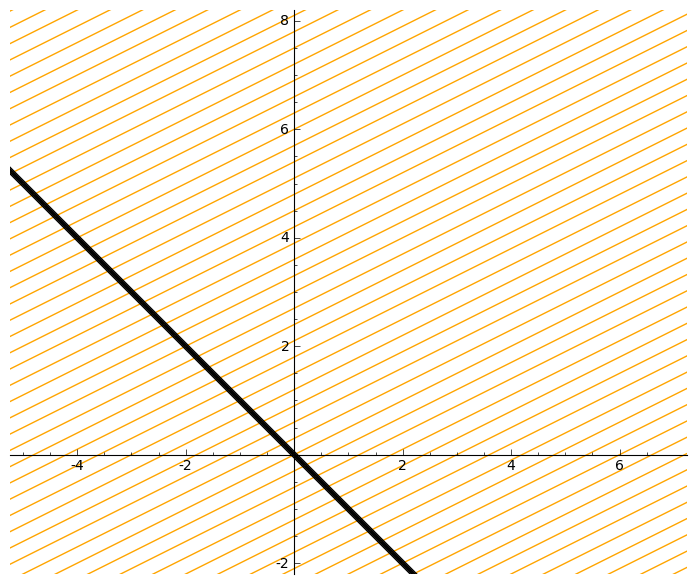
\includegraphics[width=\marginparwidth]{road-corn}}   
\begin{enumerate}
 \item 
What does the vector equation 
$$\pvec{-1\\1}x+\pvec{2\\1}y=\pvec{6\\8}$$ 
have to do with Sally's problem.
 \item 
How would you rephrase the above equation using the language of linear combinations.  Which vector is a linear combination of which vectors?
 \item 
Find values for $x$ and $y$ that make this equation valid.
%\item 
%How far does Sally travel along the road (find the length of $\pvec{-1\\2}x$)?  How far does she travel in the corn?
\end{enumerate}
\end{problem}

The geocaching problem above requires that Sally find out how to obtain the vector $(6,8)$ as a linear combination of the vectors $(-1,1)$ and $(2,1)$.  These two vectors (the road and corn rows) gave us two directions that are independent of each other.  Each direction provides us with a new way to travel that we could not do before. There is only one way to get to the treasure at $(6,8)$ if these are Sally's only two ways to move. Let's examine what happens if we add a third direction, via some irrigation pipes.


\begin{problem}\label{salley in corn field with 3 directions}
 Assume the same conditions as the previous problem. However, now let's assume that in the corn field there are irrigation pipes following the vector $(1,1)$.  Sally now has the option to follow the road $(-1,1)$, the rows of corn $(2,1)$, or the irrigation pipes $(1,1)$. She still wants to get to the treasure at $(6,8)$, but now had 3 options for ways to travel. 
\begin{enumerate}
 \item To get to the treasure, Sally needs to write $(6,8)$ as a linear combination of the vectors $(-1,1)$, $(2,1)$, and $(1,1)$, i.e. she needs to solve
\marginpar{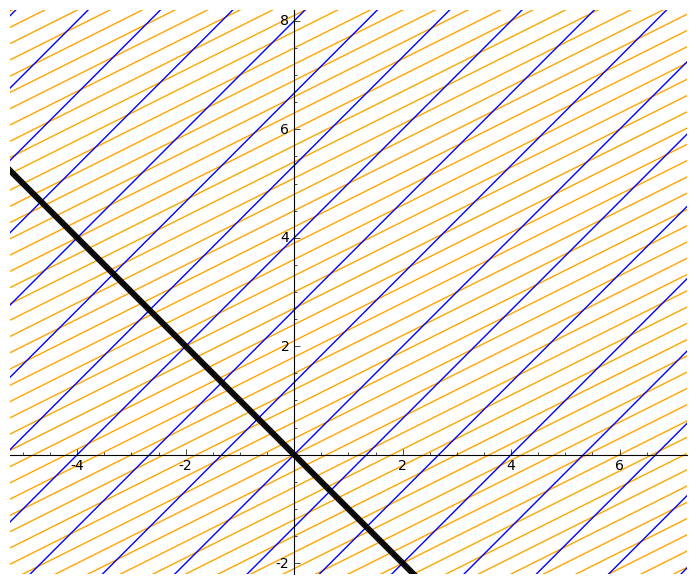
\includegraphics[width=\marginparwidth]{road-corn-pipes}}   
$$\pvec{-1\\1}x+\pvec{2\\1}y+\pvec{1\\1}z=\pvec{6\\8}.$$ 
One such option is $x=3$, $y=4$, and $z=1$.   
Find 3 different ways for Sally to get from the origin $(0,0)$ to the treasure at $(6,8)$. 
 \item Can you find a way to express every possible option that Sally has?
\end{enumerate}
\end{problem}


\mysubsection{\ideagau}

%{\huge This should be up by 4pm today.}
Every time we want to solve a problem involving linear combinations, we can convert that problem into a system of equations.
For example, if we want to write $\pvec{-4\\-15\\9}$ as a linear combination of $\pvec{1\\2\\-1}$, $\pvec{3\\4\\-2}$, and $\pvec{-2\\-10\\6}$, then we would write 
$$ 
\pvec{1\\2\\-1}x_1+\pvec{3\\4\\-2}x_2+\pvec{-2\\-10\\6}x_3=\pvec{-4\\-15\\9}
\quad \text{or}\quad
\bvec{\nvec{1\\2\\-1}&\nvec{3\\4\\-2}&\nvec{-2\\-10\\6}}\bvec{x_1\\x_2\\x_3}=\bvec{-4\\-15\\9},
$$
which as a system of equations becomes
\begin{align*}
x_1+3x_2-2x_3&=-4 \\
2x_1+4x_2-10x_3&=-15 \\
-1x_1-2x_2+6x_3&=9 
\end{align*}

You've solved systems of this form in the past. In this chapter we'll learn an efficient algorithm for solving these systems.

\begin{problem}[Organized Substitution]
Our goal on this problem is to solve the system of equations 
\begin{align*}
x+3y-2z&=-4 \\
2x+4y-10z&=-15\\
-1x-2y+6z&=9. 
\end{align*}
To solve this system, we'll use organized substitution. 
\begin{enumerate}
 \item The first equation is easy to solve for $x$. Solve for $x$ and circle your result. Then replace $x$ with this in both of the other equations. After substituting, you should be able to rewrite each equation in the form $0x+?y+?z=?$.
 \item One of these two simplified equations is easy to solve for $y$.  Solve this equation for $y$ (you shouldn't need fractions), and write your answer in the form $y=?z+?$. Circle this result.  Use this to replace $y$ in the other equation and simplify so you have $0x+0y+?z=?$. 
 \item At this point you should be able to solve for $z$. Circle your result.  Then use this result to find $y$ in your circled equation for $y$.  Then use both values for $z$ and $y$ to obtain $x$ in your circled equation for $x$.   If you ended up with $z=3/2$, then you're on the right track. 
\end{enumerate}
\end{problem}



\begin{problem}[Gaussian Elimination]
We'll now use elimination to solve the system of equations 
\begin{align*}
x+3y-2z&=-4 \\
2x+4y-10z&=-15 \\
-1x-2y+6z&=9. 
\end{align*}
\begin{enumerate}
 \item 
\marginpar{Start by making sure that the coefficient in front of $x$ on the top row is not zero. Swap rows if needed, and then multiply both sides of the top equation by a constant so that you have a 1 in this spot. Then add a multiple of this equation to every other equation to eliminate $x$ from the other equations. }%
The first equation has a 1 as the coefficient in front of $x$. Add a multiple of the first equation to every other equation so that you eliminate the $x$ variable from the other equations.
Write your system in the form 
\begin{align*}
x+3y-2z&=-4 \\
0x+?y+?z&=? \\
0x+?y+?z&=?. 
\end{align*}
 \item One of these two simplified equations is easy to solve for $y$. If you need to swap equations 2 and 3, or multiply both sides of an equation by some constant, do so now so that you can rewrite the system in the form 
\marginpar{If you ignore the top row and the variable $x$, then at this point we just repeat the above process with $y$. Make sure the coefficient in front of $y$ is 1, and then add multiples of the second equation to each lower equation to eliminate $y$.}%
\begin{align*}
x+3y-2z&=-4 \\
0x+1y+?z&=? \\
0x+?y+?z&=?. 
\end{align*}
Then add a multiple of the second equation to the third equation so that you eliminate the $y$. 
Rewrite your system in the form 
\begin{align*}
x+3y-2z&=-4 \\
0x+y+?z&=? \\
0x+0y+?z&=?. 
\end{align*}
\item 
\marginpar{We now ignore the top 2 rows and variables $x$ and $y$, and then repeat the elimination process again. We make sure to get the coefficient in front of $z$ to be a 1. Since there are no more rows beneath this third, we are done. If there had been more rows, we would just keep going.  }%
Multiply the third equation by some nonzero constant so that the coefficient in front of $z$ is a 1. Rewrite the system one final time as
\begin{align*}
x+3y-2z&=-4 \\
0x+y+?z&=? \\
0x+0y+z&=?. 
\end{align*}
 You now have $z$. Use your value for $z$ to quickly obtain $y$ from the second equation, and then $x$ from the first equation.
\end{enumerate}
\end{problem}



\begin{observation}
 
When solving the above system with substitution, we 
\begin{enumerate}
 \item 
picked an equation for which it was easy to solve for a variable, 
 \item
solved for that variable, and then 
\item
replaced that variable in the other equations and simplified each equation. 
\end{enumerate}
We then leave the picked equation alone, and repeat this process on the remaining simplified equations. 

When solving the above system with elimination, we 
\begin{enumerate}
 \item 
picked an equation that we could use to eliminate a variable from the other equations, interchanging this equation with one higher up if needed, 
 \item
multiplied the chosen equation by a nonzero constant to make the leading coefficient 1, and then 
 \item 
added a multiple of the chosen equation to the other equations to eliminate the variable from the other equations. 
\end{enumerate}
We then left the picked equation alone, and repeated this process on the remaining simplified equations below it. 
\end{observation}

These two processes (organized substitution and Gaussian elimination) are fundamentally the same process. You should have noticed that your intermediate steps were the same. We now develop a way to replicate both of these processes with matrices.

\begin{problem}[Gaussian Elimination with Matrices]\
%\marginpar{Follow this link to watch a video of how to perform Gaussian elimination with matrices.}%
Let's solve the same system 
\begin{align*}
x+3y-2z&=-4 \\
2x+4y-10z&=-15 \\
-1x-2y+6z&=9. 
\end{align*}
but now we will only write the coefficients of our system in a matrix. The matrix helps us organize our work, and we have less to write. 
\begin{enumerate}
\item 
\marginpar{This matrix is called the augmented matrix of the system. The vertical bar you see is optional, and is often used to help people remember that there is an equal sign there.} % 
Start by writing the coefficients of system in the matrix (fill in the blanks) 
$$\bvec{[ccc|c]
1 & 3 & -2 & -4 \\
2 & ? & ? & -15 \\
? & ? & 6  & ?}.
$$
\item 
\marginpar{I often write the row operation next to the row I am about to replace. }
Since the upper left entry is a 1, we are ready to reduce.  Add a multiple of row 1 to both row 2 and row 3 (replacing the old row 2 and 3) so that you obtain a zero in both entries below the leading 1 in the top row. Write your work as
$$
\nvec{\bvec{[ccc|c]
1 & 3 & -2 & -4 \\
2 & ? & ? & -15 \\
? & ? & 6  & ?}
\nvec{[l] \\ R_2-2R_1   \\ R_3+?R_1 }
}
\Rightarrow
\nvec{\bvec{[ccc|c]
1 & 3 & -2 & -4 \\
0 & ? & -6 & ? \\
0 & 1 & ?  & ? }
}.
$$
 \item Swap $R_2$ and $R_3$. This should get you a $1$ as the first nonzero entry in row 2. Then you can add a multiple of row 2 to row 3 to obtain a zero below this 1. Write your work in the form 
$$
\nvec{\bvec{[ccc|c]
1 & 3 & -2 & -4 \\
0 & ? & -6 & ? \\
0 & 1 & ?  & ? }
\nvec{[l] \\ R_2\leftrightarrow R_3   \\  }
}
\Rightarrow
\nvec{\bvec{[ccc|c]
1 & 3 & -2 & -4 \\
0 & 1 & ? & ? \\
0 & ? & -6  & ? }
\nvec{[l] \\ \\ R_3+?R_2 }}
\Rightarrow
\nvec{\bvec{[ccc|c]
1 & 3 & -2 & -4 \\
0 & 1 & ? & ? \\
0 & 0 & ?  & 3 }
}
.
$$
 \item Multiply row 3 by some nonzero constant so that the first nonzero entry in row 3 is a 1.  Write your work as
$$
\nvec{\bvec{[ccc|c]
1 & 3 & -2 & -4 \\
0 & 1 & ? & ? \\
0 & 0 & ?  & ? }
\nvec{[l] \\ \\ ?R_3 }}
\Rightarrow
\nvec{\bvec{[ccc|c]
1 & 3 & -2 & -4 \\
0 & 1 & ? & ? \\
0 & 0 & 1  & ? }
}
$$ 
\item Now rewrite your matrix as a system of equations.  The last line row of your matrix, after rewriting it as a system, should be $z=3/2$. Use this to find $y$ and $x$. 
\end{enumerate}
\end{problem}

In our work above, our process was precisely the same as when we used elimination without matrices. When working with equations, we can always (1) interchange the order of equations without changing the solution set to the system.  We can also (2) multiply both sides of an equation  by a nonzero number without affecting the solutions.  Finally, (3) adding a multiple of one equation to another will not affect the solution set. When working with matrices, these three operations on equations become operations on rows of a matrix.  

\begin{definition}[Row Operations]
We define allowed row operations.
\begin{enumerate}
  \item Interchange two rows.
  \item Multiply a row of a matrix by a nonzero constant.
  \item Add a nonzero multiple of a row to another row.
\end{enumerate}
\end{definition}

The row operations above are precisely what we used to row reduce our matrix. The elimination process begins with the first column. We obtain a 1 in the top of that column by (1) swapping rows and/or  (2) multiplying a row by a nonzero scalar. We then (3) add multiples of the first row to the other rows to obtain zeros below this leading 1.  We then ignore the row and column containing this leading 1, and repeat the reduction on the remaining part of the matrix. We can summarize the reduction algorithm with the diagram below.
$$
\bvec{[ccc|c]
* & * & * & * \\
* & * & * & * \\
* & * & * & * \\
}
\Rightarrow
\bvec{[ccc|c]
1 & * & * & * \\
0 & * & * & * \\
0 & * & * & * \\
}
\Rightarrow
\bvec{[ccc|c]
1 & * & * & * \\
0 & 1 & * & * \\
0 & 0 & * & * \\
}
\Rightarrow
\bvec{[ccc|c]
1 & * & * & * \\
0 & 1 & * & * \\
0 & 0 & 1 & * \\
}.
$$
The matrix at the far right provides us with enough information to quickly obtain a solution. After reducing the matrix to this form, we say the matrix is in row echelon form. 

\begin{definition}[Row Echelon Form, Leading 1, Pivot Column]
We say a matrix is in row echelon form (ref) if it satisfies each of the following conditions:
\begin{itemize}
  \item each nonzero row begins with a 1 (called a leading 1),
  \item the leading 1 in each row occurs further right than the leading 1 in the row above, and
  \item any rows of all zeros appear at the bottom.
\end{itemize}
The position in the matrix where the leading 1 occurs is called a pivot.
The column containing a pivot is called a pivot column.
\end{definition}




\begin{problem}[Gauss-Jordan Elimination]
%\marginpar{See YouTube for a video }
Consider the three planes 
$2x+3y+4z=4$, 
$x+2y=6$, and 
$-x+y+2z=0$. 
Let's find the point of intersection by applying row operations to the augmented matrix
$$
A
=
\bvec{
2&3&4&4\\
1&2&0&6\\
-1&1&2&0
}.$$ We'll first obtain row echelon form, and then continue reducing the matrix until we obtain what is called reduced row echelon form. See the link on the right if you would like to watch a video of this reduction process.
\begin{enumerate}
 \item Apply Gaussian elimination to obtain a row echelon form for $A$. You should start by interchanging the first and second rows, so that you have a 1 in the upper left. Remember the pattern 
\marginpar{We say a matrix is in row echelon form when (1) each nonzero row begins with a leading 1, (2) a leading 1 appears to the right of any leading one above it, and (3) any rows of all zeros appear at the bottom.}
$$
\bvec{
2&3&4&4\\
1&2&0&6\\
-1&1&2&0
}
\Rightarrow
\bvec{[ccc|c]
1 & * & * & * \\
0 & * & * & * \\
0 & * & * & * \\
}
\Rightarrow
\bvec{[ccc|c]
1 & * & * & * \\
0 & 1 & * & * \\
0 & 0 & * & * \\
}
\Rightarrow
\bvec{[ccc|c]
1 & * & * & * \\
0 & 1 & * & * \\
0 & 0 & 1 & * \\
}
$$
\item Let's now use row operations (instead of back substitution) to find the solution.  Starting on the right, and working left, use the 1's in each pivot column to reduce the matrix.  Use the pattern 
\marginpar{We say a matrix is in reduced row echelon form when the matrix is in row echelon form, and there are zeros above each pivot. }
$$
\bvec{[ccc|c]
1 & * & * & * \\
0 & 1 & * & * \\
0 & 0 & 1 & * \\
}
\Rightarrow
\bvec{[ccc|c]
1 & * & {\bf 0} & * \\
0 & 1 & {\bf 0} & * \\
0 & 0 & 1 & * \\
}
\Rightarrow
\bvec{[ccc|c]
1 & {\bf 0} & 0 & * \\
0 & 1 & 0 & * \\
0 & 0 & 1 & * \\
}
$$
to complete your reduction. State the point of intersection of the planes.
\marginpar{Check your answer with the technology link \href{http://bmw.byuimath.com/dokuwiki/doku.php?id=visualizing\_systems\_of\_equations}{Visualizing Systems of Equations}.}
\end{enumerate}
\end{problem}


The process above is called Gauss-Jordan elimination. The forward phase of reduction results in a matrix in row echelon form.  We then work backwards starting with the right most pivot column, and use the leading 1 to eliminate the zeros above it.

\begin{definition}[Reduced Row Echelon Form (rref)]
We say that a matrix is in reduced row echelon form (rref) if 
\begin{itemize}
\item the matrix is in row echelon form, and 
\item each pivot column contains all zeros except for the leading 1 in the pivot.
\end{itemize}
\end{definition}

The row reduction process we've described above may not always result in a unique solution. 

\begin{problem}
On this problem, you'll be using software to obtain the rref of a matrix.  The Sage command is ``A.rref()'' and the Mathematica command is ``RowReduce.'' 
\marginpar{You can use the \href{\urlrref}{Sage RREF Calculator} to check your result. Follow the link.}%
\begin{enumerate}
 \item 
Consider the three planes $x+2y-z=3$, $2x-y+4z=0$, and $-x+2z=4$.  
Use software to obtain the reduced row echelon form (rref) for the matrix
$$
\bvec{
1&2&-1&3\\
2&-1&4&0\\
-1&0&2&4
}.
$$  
What does the reduced matrix tell you about how the planes intersect?

When you present in class, you should always write the original matrix, draw an arrow to the rref of the matrix, and write rref above your arrow. This way the class can see what matrix you reduced, and what the rref is. 
 \item
If I wanted to write the vector $(3,0,4)$ as a linear combination of the vectors $(1,2,-1)$, $(2,-1,0)$, and $(-1,4,2)$, then what should I let $c_1$, $c_2$, and $c_3$ equal so that 
$$ c_1(1,2,-1)+c_2(2,-1,0)+c_3(-1,4,2)=(3,0,4),$$ 
which we could rewrite in the easier to use column form
$$ c_1\pvec{1\\2\\-1}+c_2\pvec{2\\-1\\0}+c_3\pvec{-1\\4\\2}=\pvec{3\\0\\4}.$$
[Hint: What does this have to do with the first part?] 
 \item
Now consider the three planes $x+2y-z=3$, $2x-y+4z=0$, and $-5y+6z=-6$.  
Set up an appropriate augmented matrix (make sure you show us the matrix), and use software to verify that the reduced row echelon form is
$$
\bvec{
1 & 0 & \frac{7}{5} & \frac{3}{5} \\
0 & 1 & -\frac{6}{5} & \frac{6}{5} \\
0 & 0 & 0 & 0
}.
$$
Write the three equations represented by this rref (the third equation may seem silly). 
\item Note that the third column does not have a pivot in it. If we added the equation $z=z$ to our work above, then we could solve for $x$, $y$, and $z$ in terms of the variable $z$. 
\marginpar{Because we can choose the third variable to be anything we want, we call it a free variable. }
Write your work in the form 
$$
 \nvec{x\\y\\z}\,\nvec{=\\=\\=}\,\nvec{? \\ ? \\ z}
\quad \quad \text{and}\quad \quad 
 \pvec{x\\y\\z}=\pvec{? \\ ? \\ 1}z+\pvec{?\\?\\0}.
$$
 
\end{enumerate}

\end{problem}

\begin{definition}[Free Variable]
 The variables in a system of equations each correspond to column of the augmented matrix. Some of the columns are pivot columns, and some are not.  The variables corresponding to the nonpivot columns are called free variables.  You can choose these variables to be any number you want, and the write the solution to the system of equations in terms of the free variables. 
\end{definition}

\begin{problem}
\marginpar{Here's an applicable \href{http://www.youtube.com/watch?v=89QO4t1S-cA&feature=share&list=PL7A2089C33C8EFC84}{YouTube video}. }%
Each of the following augmented matrices requires one row operation to be in reduced row echelon form. Perform the single required row operation, and then write the solution to the corresponding system of equations in terms of the free variables.
\begin{multicols}{2}
\begin{enumerate}
	\item 
$
\begin{bmatrix}[ccc|c]
 1 & 0 & 0 & 3 \\
 0 & 0 & 1 & 1 \\
 0 & 1 & 0 & -2
\end{bmatrix}
$ [Remember, you only get one row operation.]
	\item 
$
\begin{bmatrix}[ccc|c]
 1 & 2 & 0 & -4 \\
 0 & 0 & 1 & 3 \\
 -3 & -6 & 0 & 12
\end{bmatrix}
$ [The second column won't have a pivot, so include the equation $x_2=x_2$.]
	\item 
$
\begin{bmatrix}[ccc|c]
 1 & 0 & 2 & 4 \\
 0 & 1 & -3 & 0 \\
 0 & 0 & 0 & 1
\end{bmatrix}
$
	\item 
$
\begin{bmatrix}[ccccc|c]
 0 & 1 & 0 & 7 & 0 & 3 \\
 0 & 0 & 1 & 5 & -3 & -10 \\
 0 & 0 & 0 & 0 & 1 & 2 \\
 0 & 0 & 0 & 0 & 0 & 0
\end{bmatrix}
$ [There are two free variables in this problem.  One of the free variables is $x_1$.]
\end{enumerate}
\end{multicols}
\end{problem}



Throughout the remainder of this chapter, you'll be asked to obtain the rref of many matrices. Always start by using software to obtain the result. 
\marginpar{You can use the \href{\urlrref}{Sage rref calculator} to row reduce a matrix. You can use this on any device that can access a web browser.} 
Even if the problem asks you to compute the rref by hand, please start by using software. This will save you hours of potentially wasted time. 
If you know what the final answer is, you will be able to recognize that you have made a mistake early in the reduction process.

\mysubsection{\ideaind}

Think back on the opening problems of this chapter. Sally starts at the origin $(0,0)$.   
Because Sally can follow the road $(-1,1)$, she has the ability to move away from $(0,0)$. Using the road, she can use linear combinations of $(-1,1)$ to reach any location on the line $y=-x$. 

The rows of corn $(2,1)$ allow Sally to leave the road. 
She can use a linear combination of $(-1,1)$ and $(2,1)$ to arrive at any final destination in the plane that she wants. 
We say these two vectors $(-1,1)$ and $(2,1)$ are linearly independent because they each expand the places Sally can reach. Neither depends on the other. The vectors provide independent directions.
 
Introducing the third direction of travel $(1,1)$ along the irrigation pipes does not change where Sally can travel to, rather this third vector just increases her options for how to get there. Because of this, we say that $(1,1)$ linearly depends on $(-1,1)$ and $(2,1)$. The three vectors $(-1,1)$, $(2,1)$, and $(1,1)$ are dependent.

\begin{problem}
Read the three paragraphs before this problem. Then answer the following.
\begin{enumerate}
 \item If Sally only uses the road and rows of corn, how many linear combinations of $(-1,1)$ and $(2,1)$ are there that will allow Sally to reach the origin? In other words, solve the linear combination equation $$\pvec{-1\\1}x+\pvec{2\\1}y = \pvec{0\\0}$$ by reducing an appropriate matrix. Make sure you show your reduction steps by hand. 
 \item If Sally is also allowed to use the irrigation pipes, how many linear combinations of $(-1,1)$, $(2,1)$, and $(1,1)$ are there that will allow Sally to reach the origin? Obtain the reduced row echelon form of the matrix $\bvec{-1&2&1&0\\1&1&1&0}$ to give your answer.
 \item 
\marginpar{Because this problem has an answer, we say that $(1,1)$ linearly depends on $(-1,1)$ and $(2,1)$.  }%
Write the vector $(1,1)$ as a linear combination of the vectors $(-1,1)$ and $(2,1)$, i.e. solve the equation  $$\pvec{-1\\1}x+\pvec{2\\1}y = \pvec{1\\1}.$$ 
 \item Can you think of a different third vector so that using this vector would expand Sally's final destination points beyond where she can already get to with the road $(-1,1)$ and rows of corn $(2,1)$? Explain.
\note{I am hoping for two different answers her.  I would like someone to say it's impossible.  I would also like someone to suggest a 3D vector.}
\end{enumerate}

\end{problem}



\begin{definition}[Linear Independence]
We say that a set of vectors $\{\vec v_1,\vec v_2, \ldots, \vec v_n\}$ is linearly independent if the only solution to the homogeneous system $$c_1\vec v_{1}+c_2\vec v_{2}+\ldots+c_n\vec v_{n}=\vec 0$$ is the trivial solution $c_1=c_2=\cdots=c_n=0$. 
If the vectors are not independent, then we say that the vectors are linearly dependent. 
% \item In terms of spans, we say vectors are linearly dependent when one of them is in the span of the other vectors. 
%\begin{itemize}
% \item The span of a set of vectors $\{\vec v_1,\vec v_2, \ldots, \vec v_n\}$ is all possible linear combinations of the vectors. In terms of matrices, the span of a set of vectors is all possible vectors $\vec b$ such that $A\vec x=\vec b$ for some vector $\vec x$, where the vectors $\vec v_i$ are placed in the columns of $A$.
% \item The rank of a matrix is the number of pivot columns of the matrix. To find the rank of a matrix, you reduce the matrix using Gaussian elimination until you discover the pivot columns.
%\end{itemize}
\end{definition}
When a collection of vectors is linearly dependent, it is always possible to write one of the vectors as a linear combination of the others. We say the vectors are linearly dependent because one of the vectors depends on (can be obtained as a linear combination of) the other vectors.


\begin{problem*}[9.5 (do this one)]
 Are the vectors $\vec v_1 = (1,3,5)$, $ \vec v_2=(-1,0,1)$, and $\vec v_3=(0,3,1)$ linearly independent?  Solve the system $c_1\vec v_1+c_2\vec v_2+c_3\vec v_3=\vec 0$ to answer this question. If they are dependent, then write one of the vectors as a linear combination of the others.

 Are the vectors $\vec v_1 = (1,2,0)$, $ \vec v_2=(2,0,3)$, and $\vec v_3=(3,-2,6)$ linearly independent?  Solve the system $c_1\vec v_1+c_2\vec v_2+c_3\vec v_3=\vec 0$ to answer this question.  If they are dependent, then write one of the vectors as a linear combination of the others. 

[Hint: Rewrite each of these problems as a system of 3 equations. From that system of equations, write down the corresponding augmented matrix (it will have a column of all zeros at the right).  Then use software to answer each problem.  You do  not need to show your reduction steps, rather show the matrix you reduced, and the rref.]
\end{problem*}

\begin{problem}\label{rocket booster problem}
Imagine you are in a rocket traveling through space.  The rocket has 4 boosters on it.  The boosters provide thrust in a specific direction (vector), with the ability to adjust how strong the push should be in each direction (possibly even moving backwards in that direction - a two sided booster). The 4 boosters allow movement in the directions $(1,1,2)$, $(0,1,3)$, $(2,1,1)$, and $(-2,1,0)$.
\begin{enumerate}
 \item 
\marginpar{Use the \href{http://bmw.byuimath.com/dokuwiki/doku.php?id=rref\_calculator}{Sage RREF Calculator}.}%
Start by row reducing the matrix 
$\begin{bmatrix}
1 & 0 & 2 & -2 \\
1 & 1 & 1 & 1 \\
2 & 3 & 1 & 0
\end{bmatrix}$ to determine which columns are pivot columns. Use technology to get an answer. Then show your row reduction steps by hand. 

The rest of this problem deals with interpreting your rref.  Please give answers with sentences.
 \item If the 4th booster breaks, could some linear combination of the first three rocket thrusts allow you to move in the direction of the 4th rocket? In other words, is it possible to write $(-2,1,0)$ as a linear combination of $(1,1,2)$, $(0,1,3)$, and $(2,1,1)$? Explain.
 \item If the 3rd booster breaks, show that some linear combination of the other three rocket thrusts allows you to move in the direction of the 3rd rocket. What matrix should you row reduce to answer this. Show the class the matrix you started with, and its rref. You do not need to show by hand any reduction steps. Then write $(2,1,1)$ as a linear combination of the other three vectors. 
 \item You have been asked to give advice on a new rocket design. The designers figure that as long as they pick 3 directions in which to provide thrust, they should be able to fly in any direction they want. They attach boosters which allow movement in the directions $(1,3,2)$, $(-3,1,4)$, $(0,1,1)$. Set up an appropriate matrix and use software to row reduce the matrix. What advice would you give the designers?
 \item What does any of the above have to do with linear independence and linear dependence?
\end{enumerate}
\note{In class, I would like to talk about what it would take to design a rocket so that any of the three rockets could go out, and you would still be able to move freely in space.  All they would need is an rref that I followed by a column with no zero entries.  But I would like them to figure this out.  I may just make this a problem later on. 

Follow up.  I did make it a problem later on.}
\end{problem}



 



\begin{problem}
\marginpar{Use the \href{http://bmw.byuimath.com/dokuwiki/doku.php?id=rref\_calculator}{Sage RREF Calculator}.}%
Start by finding the reduced row echelon form of the matrix
$$
B = 
\begin{bmatrix}
\nvec{2\\1}&
\nvec{6\\3}&
\nvec{-1\\1}&
\nvec{2\\5}&
\nvec{0\\1}&
\nvec{1\\0}&
\nvec{3\\3}
\end{bmatrix}.
$$
Show the steps you used to row reduce this matrix. 
The point to this problem is to help you see how this single row reduction can answer all of the questions below. 
\begin{enumerate}
 \item Write $(2,5)$ as a linear combination of $(2, 1)$ and $(-1,1)$. Remember, that when writing $c_1(2,1)+c_2(-1,1)=(1,0)$, you must solve for the unknown constants. Feel free to row reduce the augmented matrix  
$\begin{bmatrix}
\nvec{2\\1}&
\nvec{-1\\1}&
\nvec{2\\5}
\end{bmatrix}
$
with technology. You don't need to show any steps of the computation.
 \item Write $(0,1)$ as a linear combination of $(2, 1)$ and $(-1,1)$. Remember, that when writing $c_1(2,1)+c_2(-1,1)=(0,1)$, you must solve for the unknown constants. If you decide to row reduce the matrix
$\begin{bmatrix}
\nvec{2\\1}&
\nvec{-1\\1}&
\nvec{0\\1}
\end{bmatrix}
$, then use technology and don't show us any of the intermediate steps. 
 \item Continue to write each of $\pvec{1\\0}$, $\pvec{3\\3}$, and $\pvec{6\\3}$ as a linear combination of $\pvec{2\\1}$ and $\pvec{-1\\1}$. [Hint: At some point, rather than row reducing 
$\begin{bmatrix}
\nvec{2\\1}&
\nvec{-1\\1}&
\nvec{a\\b}
\end{bmatrix}
$, ask how you could use the larger matrix to answer this.]
\item The following matrix row reduces to give
$$\begin{bmatrix}
1 & 0 & 2 & 4 & 5 & 8 \\
0 & 2 & -6 & 2 & -1 & 3 \\
0 & -2 & 6 & 0 & 2 & 1
\end{bmatrix}
\xrightarrow{\text{rref}}
\begin{bmatrix}
1 & 0 & 2 & 0 & 3 & 0 \\
0 & 1 & -3 & 0 & -1 & -\frac{1}{2} \\
0 & 0 & 0 & 1 & \frac{1}{2} & 2
\end{bmatrix}
.$$
Write $(5,-1,2)$ as a linear combination of the pivot columns.
\end{enumerate}
 
\end{problem}

\begin{question}
 What connection is there between the rref of a matrix and the columns of the matrix?
\end{question}

\mysubsection{\ideaeig}
\begin{problem}
The following parts ask you to look for points in a vector field where the vector field pushes either straight outwards from the origin, or pulls straight towards the origin.
\begin{enumerate}
\item
Consider the vector field $\vec F(x,y) = \bvec{3&2\\0&2}\bvec{x\\y} = \bvec{3x+2y\\2y}$. 
Compute $\vec F(x,y)$ for each of $(x,y)$ equal to $(2,2)$, $(2,1)$, $(2,0)$, $(2,-1)$, and $(2,-2)$.  Then circle the two vectors $(x,y)$ where the output $F(x,y)$ is a linear combination of the input $(x,y)$. 
For example, if $(x,y)=(-4,2)$, then we compute $\vec F(-4,2) = (-8, 4)$ and we see that $(-8,4) = 2(-4,2)$.  We have $\vec F(x,y) = 2(x,y)$.
 \item Suppose you knew that there was a direction in which the vector field 
$\vec F(x,y) = \bvec{2&5\\4&1}\bvec{x\\y} = \bvec{2x+5y\\4x+y}$ causes a radial push outwards of 6 units. This would mean there exists $(x,y)\neq(0,0)$ such that 
$$\bvec{2&5\\4&1}\bvec{x\\y} = 6\bvec{x\\y}.$$
Find a nonzero vector $(x,y)$ that satisfies this equation.

[Hint: Subtract $6\bvec{x\\y}$ from both sides. Combine terms to get a new matrix to row reduce, and then row reduce the matrix. You should find there are infinitely many correct answers.] 

\end{enumerate}
\end{problem}


\begin{problem}
 Consider the matrix $A=\bvec{1&-1\\3&5}$.
\begin{enumerate}
 \item Explain why solving the problem $A\vec x = c\vec x$ can be done by row reducing the matrix $\bvec{[cc|c]1-c&-1&0\\3&5-c&0}$.
 \item Let $c=3$. Solve $A\vec x = 3\vec x$ by row reducing an appropriate matrix. How many solutions are there?
 \item Let $c=2$. Solve $A\vec x = 2\vec x$ by row reducing an appropriate matrix. How many solutions are there?
 \item  When you row reduce a matrix, what must occur for there to be infinitely many solutions?   
  Can you find another value of $c$ where there are infinitely many solutions to this problem?
\end{enumerate}

\end{problem}




\begin{problem}
Consider the matrix 
$A=\bvec{3&4\\2&1}$.  
This matrix gives us the vector field 
$\vec F(x,y) = A\bvec{x\\y}$. 
We would like to find the directions in which the vector field either pulls a point $(x,y)$ directly towards the origin, 
or pushes the point $(x,y)$ directly away from the origin.
\begin{enumerate}
 \item Explain why we seek a solution to $$ A\bvec{x\\y} = c\bvec{x\\y}$$ where $c$ is some constant. Is $(x,y)=(0,0)$ a solution to this equation.  We call this the trivial solution.
 \item Subtract $c\bvec{x\\y}$ from both sides above.  Show that to find a nonzero $(x,y)$, we need to row reduce the matrix $\bvec{[cc|c]3-c&4&0\\2&1-c&0}$. Then use row operations to eliminate the 2 in the lower left of the matrix. [Hint: Take row 2 and multiply it by $(3-c)$.  Then add $-2$ times row 1 to row 2.]
 \item We already know that $(x,y)=(0,0)$ is a solution.  We want a nonzero solution $(x,y)$. Explain why the bottom row must reduce to be all zeros?
 \item By forcing the bottom row to consist of all zeros, you should have a quadratic equation involving $c$. Solve this equation for $c$.  
 These are the scalars for which you can find a vector that either pushes directly out or pulls directly in. 
\end{enumerate}
\end{problem}

The numbers $c$ that you computed above are called eigenvalues. Note that to find the eigenvalues, we wanted to row reduce a matrix and obtain infinitely many solutions. We'll return to this idea throughout the chapter.  

\mysubsection{\ideamul}

When we solve equations of the form $ax=b$ with numbers, we simply multiply both sides by $\frac{1}{a}$ to obtain $x=\frac{1}{a}b$. This is because for any nonzero number $a$, we have an inverse $a^{-1}$ such that $a^{-1}a = 1=aa^{-1}$. 
 
\begin{definition}[$I_n$ and $A^{-1}$]
 The identity matrix $I$ is a square matrix so that if $A$ is a square matrix, then $IA=AI=A$. The identity matrix acts like the number 1 when performing matrix multiplication. We write 
$$I_2 = \bvec{1&0\\0&1}, 
\quad I_3 = \bvec{1&0&0\\0&1&0\\0&0&1},
\quad I_4 = \bvec{1&0&0&0\\0&1&0&0\\0&0&1&0\\0&0&0&1},
 \text{etc.}$$ 

 If $A$ is a square matrix, then the inverse of $A$ is a matrix $A^{-1}$ where we have $AA^{-1}=A^{-1}A=I$, provided such a matrix exists.
\end{definition}



\begin{problem}
Let 
$A=
\begin{bmatrix}
\nvec{1\\3}&
\nvec{2\\4}
\end{bmatrix}
.$
We now develop an algorithm for computing the inverse $A^{-1}$.
If an inverse matrix exists, then we know it's the same size as $A$, so we could let $A^{-1}=\begin{bmatrix}\vec v_1 & \vec v_2\end{bmatrix}$ be the inverse matrix, where $\vec v_1$ and $\vec v_2$ are the columns of $A^{-1}$.  
\begin{enumerate}
 \item  We know that $A A^{-1} = \begin{bmatrix}\nvec{1\\0}&\nvec{0\\1}\end{bmatrix}.$ 
Explain why $A\vec v_1=\pvec{1\\0}$ and $A\vec v_2=\pvec{0\\1}$.
 \item Solve the matrix equations $A\vec v_1=\pvec{1\\0}$ and $A\vec v_2=\pvec{0\\1}$ by row reducing 
$
\begin{bmatrix}[cc|c]
\nvec{1\\3}&
\nvec{2\\4}&
\nvec{1\\0}
\end{bmatrix}
$
and 
$
\begin{bmatrix}[cc|c]
\nvec{1\\3}&
\nvec{2\\4}&
\nvec{0\\1}
\end{bmatrix}
$.
 \item What is the reduced row echelon form of
$
\begin{bmatrix}[cc|cc]
\nvec{1\\3}&
\nvec{2\\4}&
\nvec{1\\0}&
\nvec{0\\1}
\end{bmatrix}
$? How is this related to your previous work?
 \item State the inverse of $A$. 
\end{enumerate}

\end{problem}

In the previous problem we showed how to obtain a matrix $B$ so that $AB=I$. We now have an algorithm for finding the inverse matrix $A^{-1}$. We augment $A$ by the identity matrix, and then row reduce $[A|I]$ to the matrix $[I|A^{-1}]$.  The inverse shows up instantly after row reduction.


\begin{problem}
 Use the algorithm described immediately before this problem to compute the inverse of 
$$A=\begin{bmatrix}
 3 & 1 & -11 \\
 0 & -1 & 1 \\
 1 & 0 & -4
\end{bmatrix}.$$
Use technology to show you the rref of $[A|I]$, or just use A.inverse() in Sage, or Inverse[A] in Mathematica.  
Then show your row reduction steps by hand.

Once you have obtained the inverse, use your work to write $(1,0,0)$ as a linear combination of the columns of $A$.  
\end{problem}


\mysubsection{\ideaind}


\begin{problem}
For each collection of vectors, use software to determine if the collection of vectors is linearly independent or linearly dependent.  If the vectors are linearly dependent, write one of the vectors as a linear combination of the others. Do not row reduce the matrices by hand, rather on each problem first show the matrix you would row reduce, and then give the reduced row echelon form by using technology.
\begin{enumerate}
 \item $(1,0,0)$, $(0,1,1)$, $(2,3,2)$, and $(0,1,-1)$ 
[Remember, the vectors are linearly independent if the only solution to 
$$\pvec{1\\0\\0}c_1+\pvec{0\\1\\1}c_2+\pvec{2\\3\\2}c_3+\pvec{0\\1\\-1}c_4=\pvec{0\\0\\0}$$ is the trivial solution $c_1=c_2=c_3=c_4=0$.]
 \item $(1,0,2,0)$, $(0,1,3,1)$, and $(0,1,2,-1)$
 \item $(1,1,2,-1)$, $(-3,1,4,1)$, and $(-1,1,3,0)$
 \item Suppose you have 5 vectors that are each 7 tall. Row reducing the 7 by 5 matrix obtained by placing these vectors in columns results in a matrix that has 3 rows of zeros at the bottom.  Why are the vectors linearly dependent?
 \item If you have a matrix with $n$ rows and $m$ columns, what must happen for the column vectors to be linearly independent?  How many rows of zeros would be at the bottom if the vectors are linearly independent. 
\end{enumerate}
[Hint: For all parts, think about the number of pivot columns.]
\end{problem}





\begin{problem}[Rocket Booster Design]
\marginpar{If you are worried about rotation that might occur from firing these boosters, then please imagine that each booster applies a force through the center of mass of the object, so that no rotation occurs.  }%
Three teams have been asked to design a space suit that allows for travel in space. As part of the project requirements, the teams are required to use 4 two-way boosters for propulsion.  The 4th booster is there to allow for redundancy in case any of the the other boosters break. 
\begin{itemize}
 \item Team 1 decides to add boosters to their suit that allows for travel in the directions 
$[1,-1,1],
[1,2,-1],
[3,-1,2],
[1,1,0]$.
 \item Team 2 decides to add boosters to their suit that allows for travel in the directions 
$[1,-3,2],
[0,1,1],
[-1,3,2],
[1,-1,3]$.
 \item Team 3 decides to add boosters to their suit that allows for travel in the directions
$[1,1,-2],
[3,-1,4],
[2,0,1],
[1,-3,8]$.
\end{itemize}
For each team, use software to row reduce the appropriate 3 by 4 matrix that would tell the dependence relationships among the vectors. If you were in charge of picking a winning design, which team would you pick, and why?
\end{problem}


\mysubsection{\ideamul}

\begin{problem}
Start by writing the system of equations 
\begin{align*}
 -2x_1+ 5x_3 &=-2\\
 -x_1+ 3x_3 &=1\\
 4x_1 +x_2  -x_3 &=3
\end{align*} 
as a matrix product $A\vec x =\vec b$.  (What are $A$, $\vec x$ and $\vec b$?)  
\begin{enumerate}
\item 
\marginpar{You should use technology to rapidly compute the inverse and also row reduce the augmented system.  Show by hand any matrix computations you do on  part 3. }%
Use software to find the inverse of the matrix $A$ (state the matrix you row reduced, and the rref of the matrix). 
\item Use software to row reduce the augmented matrix $\begin{bmatrix}[c|c]A&\vec b \ \end{bmatrix}$. State the rref.
\item To solve the problem $ax=b$ where $a$, $x$, and $b$ are numbers, we multiply both sides by $\frac{1}{a}$ to obtain $\frac{1}{a}ax=\frac{1}{a}b$, or because $\frac{1}{a}a=1$, we simplify to get $x=\frac{1}{a}b$. How can you use this idea to solve the matrix problem $A\vec x = \vec b$?  Show how to obtain the solution to this system by using the matrix inverse. 
\item Does it matter if you compute $\vec b A^{-1}$ or  $A^{-1}\vec b$?
%\item What differences do think there are
%$\vec x = \dfrac{1}{A}\vec b$, $\vec x = \dfrac{\vec b}{A}$, and $\vec x = \vec b\dfrac{1}{A}$?   
\end{enumerate}
\end{problem}
\note{At this point I want to talk about order of matrix multiplication.  But it will become much more apparent later on.}



\begin{problem}\label{inverse of 2 by 2}
\marginpar{[Hint: Because the matrix has variables in it, you may want to try a different scheme for row reducing.  Multiply the top row by $c$ and the bottom row by $a$. Then subtract the top row from the bottom. This gets you a zero below the pivot in the first column. Then multiply the top row by $ad-bc$ and the bottom row by something else.]}%
Let $A=\begin{bmatrix}a&b\\c&d\end{bmatrix}$. Obtain the rref of $[A | I]$ to show that the inverse of $A$ is 
$$A^{-1}=\frac{1}{ad-bc}\begin{bmatrix}d&-b\\-c&a\end{bmatrix}.$$

Are there any conditions under which a matrix would not have an inverse?  What are they, and why? Is there a number you could check to {\it determine} if a matrix has an inverse?
\end{problem}

\mysubsection{\ideadet}
In computing the inverse of a 2 by 2 matrix, the number $ad-bc$ appears in the denominator. We call this number the determinant. 
\marginpar{Take a guess as to why we call this number the determinant.  What does it help determine?}% 
If I asked you to compute the inverse of a 3 by 3 matrix, you would again see a number appear in the denominator.  We call that number the determinant. This holds true in all dimensions.

\begin{problem*}[Optional]
  Let $A=\begin{bmatrix}a&b&c\\d&e&f\\g&h&i\end{bmatrix}$. Use Gauss-Jordan elimination to find the inverse of $A$, and show that the common denominator is $a(ei-hf)-b(di-gf)+c(dh-ge)$. 
\end{problem*}


\begin{definition}[Determinants of 2 by 2 and 3 by 3 matrices]\label{determinat of 2 by 2 and 3 by 3}
\marginpar{In Sage, we've been using A.rref() to get the reduced row echelon form of $A$. You can type A.determinant() to get the determinant. Similarly, A.inverse() will get you the inverse. }
 The determinant of a {$2\times 2$} and {$3\times 3$} matrix are the numbers 
\begin{align*}
\det\begin{bmatrix}a&b\\c&d\end{bmatrix} &=\begin{vmatrix}a&b\\c&d\end{vmatrix} = ad-bc\\
\begin{vmatrix}a&b&c\\d&e&f\\g&h&i\end{vmatrix} &= a\det\begin{vmatrix}e&f\\h&i\end{vmatrix} -b\det\begin{vmatrix}d&f\\g&i\end{vmatrix} +c\det\begin{vmatrix}d&e\\g&h\end{vmatrix}\\
&=a(ei-hf)-b(di-gf)+c(dh-ge)
\end{align*}
\marginpar{This approach generalizes to give the determinant of any square matrix.  More on this soon. }% 
We use vertical bars next to a matrix to state we want the determinant. Notice the negative sign on the middle term of the {$3 \times 3$} determinant. 
Also, notice that we can compute three determinants of 2 by 2 matrices in order to find the determinant of a 3 by 3. 
\end{definition}










\begin{problem}
The columns of each matrix below provide the edges of the parallelogram beneath the matrix.
\begin{center}
 \begin{tabular}{ccccc}

$A=\bvec{2&0\\0&3}$
&$B=\bvec{2&1\\0&3}$
&$C=\bvec{1&2\\4&0}$
&$D=\bvec{-2&1\\1&2}$
&$E=\bvec{1&-2\\2&1}$\\\hline
\begin{tikzpicture}[scale=.5] 
\draw[->,very thick] (0,0) -- (2,0); \draw[->,very thick] (0,0) -- (0,3); 
\draw[->] (0,3) -- (2,3); \draw[->] (2,0) -- (2,3); 
\end{tikzpicture}
&\begin{tikzpicture}[scale=.5] 
\draw[->,very thick] (0,0) -- (2,0); \draw[->,very thick] (0,0) -- (1,3); 
\draw[->] (1,3) -- (3,3); \draw[->] (2,0) -- (3,3); 
\end{tikzpicture}
&\begin{tikzpicture}[scale=.5] 
\draw[->,very thick] (0,0) -- (1,4); \draw[->,very thick] (0,0) -- (2,0); 
\draw[->] (1,4) -- (3,4); \draw[->] (2,0) -- (3,4); 
\end{tikzpicture}
&\begin{tikzpicture}[scale=.5] 
\draw[->,very thick] (0,0) -- (-2,1); \draw[->,very thick] (0,0) -- (1,2); 
\draw[->] (-2,1) -- (-1,3); \draw[->] (1,2) -- (-1,3); 
\end{tikzpicture}
&\begin{tikzpicture}[scale=.5] 
\draw[->,very thick] (0,0) -- (-2,1); \draw[->,very thick] (0,0) -- (1,2); 
\draw[->] (-2,1) -- (-1,3); \draw[->] (1,2) -- (-1,3); 
\end{tikzpicture}
\end{tabular}
\end{center}

\begin{enumerate}
\item Compute the determinant of each matrix above. What happens to the determinant when you switch the order of the columns? 
\item Use geometric reasoning to compute the area of each parallelogram ($A=bh$). For the last two, note that the vectors $(-2,1)$ and $(1,2)$ are orthogonal, so the parallelogram is a square. Find the length of each side. 
\item For each parallelogram above, decide if you have to rotate clockwise or counterclockwise to get from the vector in the first column to the vectors in the second column. What does this have to do with the sign of the determinant?
\item Consider the matrix $F=\bvec{ \nvec{3\\2}&\nvec{4\\-1} }$.  Draw the corresponding parallelogram and make a guess as to whether or not the determinant is positive or negative (without computing it). Then compute the determinant and use it to guess the area of the triangle with vertices $(0,0)$, $(3,2)$, and $(4,-1)$.
\end{enumerate}
\end{problem}

The problem above uses inductive reasoning (lots of examples) to suggest that the determinant of a matrix (up to a sign) is the area of a parallelogram. This next problem asks you to use deductive reasoning to prove that the determinant of a 2 by 2 matrix gives the area of a parallelogram whose edges are the columns of the matrix.
\begin{problem}
 To find the area of the parallelogram with vertexes $O=(0,0)$, $P=(a,c)$, $Q=(b,d)$, and $R=(a+b,c+d)$, we need to find the length of $OP$ (the base $b$), and multiply it by the distance from $Q$ to $OP$ (the height $h$). Let $\vec b = \vec{OP}$ and let $\vec h$ be the shortest vector from the line $OP$ to the point $Q$. Complete the following:
\begin{enumerate}
 \item Find the projection of $\vec {OQ}$ onto $\vec {OP}$. (You may need to look up a vector projection formula.) Part of this formula requires that you compute the length of $\vec b$.  
 \item Recall that we can obtain the vector $\vec h$ by computing $\vec h = \vec {OQ}-\text{proj}_{\vec{OP}}\vec{OQ}$. We call this vector is the vector component of $\vec {OQ}$ that is orthogonal to $\vec {OP}$. Compute $\vec h$.
 \item The length of $\vec h$ is the distance $h$ from $Q$ to $OP$. Find the length of $\vec h$.
 \item We now have $b$ and $h$. Compute the product and simplify to show that the area of the parallelogram is $|ad-bc|$.
\end{enumerate}
\end{problem}

The result above extends to 3 dimensions.  The determinant of a 3 by 3 matrix gives the volume of the parallelepiped whose edges are the columns of the 3 by 3 matrix. Because this result holds true in 1, 2, and 3 dimensions, we can use the determinant to define an $n$th dimensional volume. This is precisely what happens in practice. 




\mysubsection{\ideaeig}

There is a connection between linear independence and the determinant.


\begin{problem}
Consider the matrices $A=\bvec{1&-2\\2&-4}$,  $B=\bvec{2&-1\\4&3}$, and $C=\bvec{-2-\lambda&1\\3&4-\lambda}$. (Note that $C = \bvec{-2&1\\3&4}-\lambda \bvec{1&0\\0&1}$.)   
\begin{enumerate}
 \item Compute the determinants of $A$, $B$, and $C$. \marginpar{The determinant of $C$ is called the characteristic polynomial of $\bvec{-2&1\\3&4}$.}
 \item Are the columns of $A$ linearly independent or linearly dependent? Explain.  
 \item Are the columns of $B$ linearly independent or linearly dependent? Explain.
 \item Make a conjecture about determinants and linear independence.  
 \item Find two different values $\lambda$ so that $C$ has linearly dependent columns. (Your answer should involve irrational numbers.)
\end{enumerate}
\end{problem}


A main goal in this chapter has been to answer the following two questions:
\begin{enumerate}
 \item For which nonzero vectors $\vec x$ (eigenvectors) is it possible to write $A\vec x = \lambda \vec x$?
 \item Which scalars $\lambda$ (eigenvalues) satisfy $A\vec x = \lambda \vec x$?
\end{enumerate}
These questions are precisely connected to when a vector causes a radial push away or pull towards the origin. 
Let's give some formal definitions.



\begin{definition}[Eigenvector, Eigenvalue, Characteristic Polynomial]
Let $A$ be a square $n\times n$ matrix. 
\begin{itemize}
 \item An eigenvector of $A$ is a nonzero vector $\vec x$ such that $A\vec x =\lambda \vec x$ for some scalar {$\lambda$}. (Matrix multiplication reduces to scalar multiplication.) We avoid letting $\vec x$ be the zero vector because it is trivially true that $A\vec 0=\lambda \vec 0$ no matter what $\lambda$ is.
 \item If $\vec x$ is an eigenvector with $A\vec x = \lambda \vec x$, then we call $\lambda$ an eigenvalue of $A$.
 \item We call $\det(A-\lambda I)$ the characteristic polynomial of $A$.  It is a polynomial in $\lambda$ of degree $n$, hence has $n$ roots (counting multiplicity).  These roots are the eigenvalues of $A$.
\end{itemize}
\end{definition}




\begin{problem}
 Consider the matrix $A=\bvec{5&6\\3&-2}$. 
\begin{enumerate}
 \item Show that the eigenvalues are $\lambda = 7$ and $\lambda = -4$. You'll want to compute the determinant of $A-\lambda I = \bvec{5-\lambda&6\\3&-2-\lambda}$
 \item If we let $\lambda = 7$, find a nonzero vector $\vec x = (x,y)$ such that $A\vec x = 7\vec x$. You'll need to row reduce $\bvec{[cc|c]5-7&6&0\\3&-2-7&0}$.  
 \item If we let $\lambda = -4$, find a nonzero vector $\vec x = (x,y)$ such that $A\vec x = -4\vec x$.  
 \item If $\lambda = 6$, then what is the only solution $\vec x = (x,y)$ to $A\vec x = 6\vec x$? [Hint: this one can be answered without doing any row reduction.] 
\end{enumerate}

\end{problem}


\begin{problem}
Consider the matrix 
$A=
\begin{bmatrix}
 3 & 1 \\
 4 & 6
\end{bmatrix}
$.
 \begin{enumerate}
 \item Find the characteristic polynomial of $A$, and use it to determine the eigenvalues of $A$. 
 \item For each eigenvalue, find all corresponding eigenvectors. 
% \item Compute the trace and determinant of $A$.
\end{enumerate}
\end{problem}




\begin{problem}
Consider the matrix 
$
A=
\begin{bmatrix}
 6 & 4  \\
 3 & 2  
\end{bmatrix}
$. 
Find the eigenvalues of $A$. 
Then for each eigenvalue, find all corresponding eigenvectors.
%(Check your work by computing the trace and determinant of $A$.)
\end{problem}







\mysubsection{\ideamul}

\begin{problem}[Encryption]
Consider the matrix 
$A =
\begin{bmatrix}
 2&1&-1\\
 5&2&-3\\
 0&2&1
\end{bmatrix}
$.  
Joe decides to send a message to Ben by encrypting the message with the matrix $A$. He first takes his message and converts it to numbers by replacing A with 1, B with 2, C with 3, and so on till replacing Z with 26.  He uses a 0 for spaces.  After replacing the letters with numbers, he breaks the message up into chunks of 3 letters.  He then multiplies each chunk of 3 by the matrix $A$, resulting in a coded message. For example, to send the message ``good job ben'' he firsts converts the letters to the numbers and places them in a large matrix $M$ (top to bottom, left to right) 
$$
\left[\bvec{g\\o\\o}, \bvec{d\\ \ \\ j},\bvec{o\\b\\\  },\bvec{b\\e\\n}\right] 
\rightarrow
\left[\bvec{7\\15\\15}, \bvec{4\\0\\10},\bvec{15\\2\\0},\bvec{2\\5\\14}\right] 
= M=
\begin{bmatrix}
7 & 4 & 15 & 2 \\
15 & 0 & 2 & 5 \\
15 & 10 & 0 & 14  
\end{bmatrix}
.$$
To encode the matrix, he computes 
$$AM = 
\begin{bmatrix}
14 & -2 & 32 & -5 \\
20 & -10 & 79 & -22 \\
45 & 10 & 4 & 24
\end{bmatrix}.$$
and then sends the numbers 
$[
[ 14,  20,  45],
[ -2, -10,  10],
[ 32,  79,   4],
[ -5, -22,  24]]
$ to Ben. Ben uses the inverse of $A$ to decode the message. 
\begin{enumerate}
 \item Find the inverse of $A$. 
 \item Use $A^{-1}$ to decode $[
[ 14,  20,  45],
[ -2, -10,  10],
[ 32,  79,   4],
[ -5, -22,  24]]$ and show the message is ``good job ben''.
 \item Decode the message $[[39, 89, 22],[20, 48,  4],[39, 88, 33]]$.
\end{enumerate}
\end{problem}




\begin{problem}
The eigenvalues of the matrix 
$A=\bvec{2&6\\18&5}$ are $\lambda_1 = 14$ and $\lambda_2 = -7$.  An eigenvector corresponding to $\lambda_1 =14$ is  $\vec x_1=(1,2)$. 
An eigenvector corresponding to $\lambda_2 = -7$ is $\vec x_2 = (-2,3)$. 
\begin{enumerate}
 \item What is the product $A\vec x_1$? What is the product $A\vec x_2$? Can you explain how to get these products without actually doing matrix multiplication.
 \item 
\marginpar{We place the eigenvectors of $A$ into the columns of $Q$.}%
What is the product $AQ$ where $Q = \bvec{\vec x_1&\vec x_2} = \bvec{1&-2\\2&3}$. You can do this product by using your answer to the first part. 
 \item 
\marginpar{[There are several ways to do this problem. You could multiply both sides on the left by the inverse of $Q$ to solve for $D$. Another way is to reason about the connection between eigenvalues, eigenvectors, the matrix $A$, and linear combinations.]
}%
Find a matrix $D$ so that $AQ=QD$.  Any idea why we use $D$ for this matrix? See the hint on the side. 

\item 
Suppose $A$ is a 3 by 3 matrix with eigenvectors $\vec x_1$, $\vec x_2$, and $\vec x_3$, corresponding to the eigenvalues $\lambda = 2,4,-5$, respectively. If we let $Q = \bvec{\vec x_1&\vec x_2&\vec x_3}$, then make a guess as to what $D$ should equal so that $AQ=QD$. Explain your guess. Guess what $D$ equals if we instead place the eigenvectors into $Q$ in the order $Q = \bvec{\vec x_2&\vec x_3&\vec x_1}$? 


\end{enumerate}
%What do they get if they compute AQ (or explain why we immediatly know AQ).  Does it equal DQ or QD.  Does order matter?
%They have to analyze what matrix multiplication means. 
\end{problem}

In the problem above, we wrote $AQ=QD$ where $D$ is a diagonal matrix whose diagonal entries are the eigenvalues of $A$. The columns of $Q$ are eigenvectors of $A$, which we place in the same order as the eigenvalues on the diagonal of $D$. We can use this idea to obtain a matrix with any desired eigenvalue/eigenvector pairs. In particular, this means we can observe something in nature and look for outward/inward pushes/pulls. From these observations we know $Q$ and $D$, which means we can solve for $A$. 


\begin{problem}
Suppose you know that the matrix $A$ has eigenvalues $\lambda_1=2$ and $\lambda_2=-3$ with corresponding eigenvectors $\vec x_1=(2,-5)$ and $\vec x_2 = (1,3)$.
\begin{enumerate}
 \item 
\marginpar{Since $AQ=QD$, what does multiplying both sides by $Q^{-1}$ on the right yield?}%
We can write $AQ=QD$ where $Q=\bvec{\nvec{2\\-1}&\nvec{1\\3}}$ and $D=\bvec{2&0\\0&-3}$. Use this information to solve for $A$.  You can get $Q^{-1}$ quickly from Problem \ref{inverse of 2 by 2}.  Your matrix $A$ should have fractional values in it, with a denominator equal to the determinant of $Q$.
 \item We could have instead written $AQ=QD$ where $Q=\bvec{\nvec{1\\3}&\nvec{2\\-1}}$ and $D=\bvec{-3&0\\0&2}$ (reversing the order we put things into $Q$ and $D$). Use this information to solve for $A$.
 \item Suppose we know that a vector field $\vec F$ applies the forces $F(4,-2) = (8,-4)$ and $F(-1,-3) = (3,9)$. Explain why we know two eigenvectors are $(4,-2)$ and $(3,9)$ with corresponding eigenvalues $\lambda=2$ and $\lambda =-3$.  Use this information to state $Q$ and $D$, and then use $AQ=QD$ to find the matrix $A$ such that $F(x,y)=A\pvec{x\\y}.$
 \item You should have gotten the exact same matrix $A$ in each problem above, though the $Q$ and $D$ used on each part was different. Guess another choice for $Q$ and $D$, different than the three above, so that $AQ=QD$. Why did you make this guess? 
%This problem is most likely best left for a discussion in class.  Let them do the computations. 
% \item We know there are infinitely many eigenvectors corresponding to each eigenvalue of $A$. When we use $AQ=QD$ to find the matrix $A$, does it matter which eigenvectors we choose to put in $Q$?  Does the order we place the eigenvectors in $Q$ make a difference?
\end{enumerate}
\end{problem}

\mysubsection{\ideadet}
Recall that the determinant of a {$2\times 2$} and {$3\times 3$} matrix are the numbers 
\begin{align*}
\det\begin{bmatrix}a&b\\c&d\end{bmatrix} &=\begin{vmatrix}a&b\\c&d\end{vmatrix} = ad-bc\\
\begin{vmatrix}a&b&c\\d&e&f\\g&h&i\end{vmatrix} &= a\det\begin{vmatrix}e&f\\h&i\end{vmatrix} -b\det\begin{vmatrix}d&f\\g&i\end{vmatrix} +c\det\begin{vmatrix}d&e\\g&h\end{vmatrix}\\
&=a(ei-hf)-b(di-gf)+c(dh-ge)
\end{align*}
Notice that we compute three determinants of 2 by 2 matrices in order to find the determinant of a 3 by 3. We now extend this to give a way to compute determinants of any matrix.


\begin{definition}[Minors, Cofactors, and General Determinants]\label{general determinants}
Let {$A$} be an $n$ by $n$ matrix. 
\begin{itemize}
 \item The minor {$M_{ij}$} of a matrix {$A$} is the determinant of the the matrix formed by removing row {$i$} and column {$j$} from {$A$}. 
 \item 
\marginpar{
%\begin{wraptable}[7]{r}{0pt}
%\small
%\begin{tabular}{c}
$\begin{bmatrix}
+&-&+&\cdots\\
-&+&-&\cdots\\
+&-&+&\cdots\\
\vdots&\vdots&\vdots&\ddots
\end{bmatrix}$ 
%\end{tabular}%\end{wraptable}

This sign matrix keeps track of the $(-1)^{i+j}$ portion in the cofactor.
}%
The cofactor $C_{ij}$ is the product of the minor $M_{ij}$ and $(-1)^{i+j}$. This gives $C_{ij} = (-1)^{i+j}M_{ij}$.
 \item To compute the determinant, first pick a row or column.
Then take each entry $a_{ij}$ in that row or column and multiply the entry by its cofactor $C_{ij}$. The determinant is the sum of these products. 

{\bf The determinant is a linear combination of the cofactors of any row or column of the matrix, where we use the entries of that row or column as the scalars.  }

Using summation notation, we can write $|A| = \sum_{k=1}^n a_{ik}C_{ik}$ (if we chose row $i$) or alternatively $|A| = \sum_{k=1}^n a_{kj}C_{kj}$ (if we chose column $j$).  
\end{itemize}
\end{definition}




\begin{problem}
 Compute the determinant of 
$
\begin{bmatrix}
 2 & 3 & -1 \\
 1 & 0 & 0 \\
 4 & 2 & 5
\end{bmatrix}
$
in 3 ways. 
\begin{enumerate}
 \item 
\marginpar{\href{http://www.youtube.com/watch?v=DiULKK1CzR0&feature=share&list=PL7A2089C33C8EFC84}{Watch this relevant YouTube video.}}%
Compute the cofactors of the first row of the matrix, and use them to obtain the determinant. Please show each step of your work, don't just skip straight to an answer. You'll need to explain what you did in class, and you can't do this if you just skip all the steps in between.
 \item Use the cofactors of the second row to obtain the determinant.
 \item Find the determinant by using a linear combination of the cofactors of the third column. 
\end{enumerate}
Note: The determinant, using a linear combination of the cofactors along the second column, is
\begin{align*}
3C_{1,2}+0C_{2,2}+2C_{3,2} 
&= (3)(-1)^{1+2}\begin{vmatrix}1&0\\4&5\end{vmatrix}+(0)(-1)^{2+2}\begin{vmatrix}2&-1\\4&5\end{vmatrix}+(2)(-1)^{3+2}\begin{vmatrix}2&-1\\1&0\end{vmatrix}\\
&= -(3)\begin{vmatrix}1&0\\4&5\end{vmatrix}+(0)\begin{vmatrix}2&-1\\4&5\end{vmatrix}-(2)\begin{vmatrix}2&-1\\1&0\end{vmatrix}\\
&=\cdots \text{(you can finish).}
\end{align*}
\end{problem}




\begin{problem}
 Compute the determinants of the matrices 
$$
A=
\begin{bmatrix}
 2 & 1 & -6 & 8 \\
 0 & 3 & 5 & 4 \\
 0 & 0 & 1 & 5 \\
 0 & 0 & 0 & -4
\end{bmatrix}
\quad\text{ and }\quad
B=
\begin{bmatrix}
 3 & 2 & 5 & -1 \\
 0 & 8 & 4 & 2 \\
 0 & -1 & 0 & 0 \\
 0 & -5 & 3 & -1
\end{bmatrix}
.$$
You can make these problems really fast if you use a linear combination of cofactors where most of the scalars are zero. 
\end{problem}







\begin{problem}

Consider the matrices 
$$
A=
\begin{bmatrix}
1 & 0 & 2  \\
1 & 1 & 1  \\
2 & 3 & 1 
\end{bmatrix}
\quad\quad\text{ and }\quad\quad
B=
\begin{bmatrix}
1 & 0 &  -2 \\
1 & 1 &  1 \\
2 & 3 &  0
\end{bmatrix}.$$
\marginpar{You can use Sage to perform all your work. First store the matrices as A and B. Then use A.inverse(), B.inverse(), A.determinant(), and B.determinant(), etc. to check.}%
These matrices are related to the rocket booster problem (Problem \ref{rocket booster problem}).
\begin{enumerate}
 \item Compute the determinants of $A$ and $B$. Show this part by hand, though you should use software to check your answer. 
 \item Row reduce $A$ and $B$. Use software and just show us the rref.
 \item Are the columns of $A$ linearly independent or linearly dependent? What about the columns of $B$?
 \item Row reduce both $[A|I]$ and $[B|I]$, and then state the inverse of each (or explain why it does not exist).  Use software and just show us the rref.   
 \item How many solutions are there to $A\vec x = \vec 0$?  How many solutions are there to $B\vec x=\vec 0$?
 \item How many solutions does 
$x\pvec{1\\1\\2}+
y\pvec{0\\1\\3}+
z\pvec{2\\1\\1}=
\pvec{0\\0\\0}
$ have?

How many solutions does 
$x\pvec{1\\1\\2}+
y\pvec{0\\1\\3}+
z\pvec{-2\\1\\0}=
\pvec{0\\0\\0}
$ have?
\item Make some conjectures about the relationships you see above. 

\end{enumerate}
\end{problem}


\begin{definition}[Singular]
 We say that a matrix is singular when the determinant of $A$ equals zero, which is precisely when the matrix does not have an inverse. 
\end{definition}






\mysubsection{\ideaeig}

Remember, to find the eigenvalues and eigenvectors of a matrix, we need to find nonzero vector solutions to $(A-\lambda I)\vec x=\vec 0$. This means the determinant of $A-\lambda I$ must be zero, which is the quick formula we use for computing eigenvalues. 

\begin{problem}
Consider the matrix 
$
A=
\begin{bmatrix}
 4 & 0 & 0 \\
 0 & 2 & 1 \\
 0 & 1 & 2
\end{bmatrix}
$. 
Show that the characteristic polynomial of $A$ is $(4-\lambda)(\lambda-3)(\lambda -1)$, and then state the eigenvalues of $A$. 
Then for each eigenvalue, find all corresponding eigenvectors. Show your row reduction steps to get the eigenvectors. (You'll need to row reduce 3 matrices, but with each one the row reduction should be quite fast as the bottom row should reduce to all zeros.)
\end{problem}

\begin{problem}\label{First example of deficient eigenvalue}
Consider the matrices
$
B=
\begin{bmatrix}
 3 & 0 & 0 \\
 0 & 2 & 1 \\
 0 & 1 & 2
\end{bmatrix}
$ and 
$
C=
\begin{bmatrix}
 3 & 1 & 0 \\
 0 & 2 & 1 \\
 0 & 1 & 2
\end{bmatrix}
$.
Feel free to use software on this problem to perform any needed row reductions. 
\begin{enumerate}
\item Show that the characteristic polynomial for both $B$ and $C$ is $(3-\lambda)(\lambda-3)(\lambda -1)$.  What are the eigenvalues?
\item For each eigenvalue of $B$, state all the corresponding eigenvectors. Show us the matrix you need to row reduce, show the rref (from software), and then state the eigenvectors by writing $(x,y,z)$ in terms of the free variables.
\item For each eigenvalue of $C$, repeat the previous step.
\item If you have a repeated eigenvalue, how many linearly independent eigenvectors should you expect to find?
\end{enumerate}
When you are done, you should have written down 4 matrices (2 for each part), each matrix's rref, and then stated the eigenvectors by writing $(x,y,z)$ in terms of the free variables on each part.  
 \end{problem}




\mysubsection{\ideagau}
Recall that there are three types of row operations, namely (1) swap rows, (2) multiply a row by a nonzero constant, and (3) add a multiple of a row to another row.  

When you row reduce the matrix $\bvec{a&b&c\\d&e&f}$ using Gauss-Jordan elimination (or any $2$ by $n$ matrix), we can count the largest number of row operations we'll ever need to perform.  Assume at each stage we decide to swap two rows to get a nice nonzero number in the pivot, and then we multiply that row by a nonzero number to obtain a leading 1. 
With a 2 by $n$ matrix, we would swap rows 1 and 2, and then multiply row 1 by a nonzero number. Then we would add a multiple of row 1 to row 2 to eliminate the entry below this leading 1. We would then multiply row 2 by a nonzero number to obtain a leading 1. Then we'd need one more row operation to eliminate the number above the pivot in column 2. This is a total of 5 operations (we swapped 1 time, multiplied a row 2 times, and added a multiple of a row to another 2 times).  

For larger matrices, how many row operations are needed to perform Gauss-Jordan elimination?
This question is extremely important to computer programming, as the answer related to the time needed for a computer to row reduce a million by million matrix, something that happens all the time since the advent of computers.

%I don't think they will care.....  I'm moving on.
\begin{problem}[Number of operations]
Here's your challenge:  How many row operations are needed to fully reduce an $m$ by $n$ matrix, where $n>m$.
\begin{itemize}
 \item For a 3 by 4 matrix, we would swap rows a maximum of 2 times (once for each row but the last).  We would need to multiply a row by some number 3 times (once for each leading 1). We would add a multiple of a row to another 3 times in the forward elimination and 3 times in the backward elimination (this puts the zeros above and below each pivot). We now have $2+3+6 = 11$ row operations.
 \item Now consider a 4 by 5 matrix. How many row swaps at most will you need?  How many times will you need to multiply to get a leading 1?  How many times will you need to add a multiple of a row to another to get a zero above or below a pivot?  List all these out, then write the number of row operations needed.
 \item Now consider a 5 by 6 matrix. Repeat the above.
 \item Now consider a 6 by 7 matrix. Repeat the above. Did you get $41$ row operations?
 \item Give a formula $f(n)$ so that for each $n$, the number $f(n)$ is the maximum number of row operations. We currently know $f(1)=1$, $f(2)=5$, $f(3)=11$, $f(4)=?$, $f(5)=?$, $f(6)=41$. 
\end{itemize}
If you've never see the online encyclopedia of integer sequences, please head to \href{http://oeis.org/}{http://oeis.org/}. Try the sequence 1, 5, 11, ....  
\end{problem}




\begin{problem}
Let $A=\bvec{6-c&2\\2&3-c}$ where $c$ is a real number.
\begin{enumerate}
 \item For which values of $c$ are the columns of $A$ linearly independent?
 \item For which values of $c$ is the matrix $A$ invertible?
 \item For which values of $c$ are there infinitely many solutions to $A\vec x = \vec 0$?
 \item For which values of $c$ is the determinant of $A$ equal to zero?
 \item For which values of $c$ does the rref of $A$ equal the identity matrix?
 \item For which values of $c$ is the matrix $A$ singular?
 \item For which values of $c$ is $\lambda=0$ an eigenvalue of $A$?
\end{enumerate}
\end{problem}


\mysubsection{\ideaeig}
There are many connections between vector fields and eigenvalues/eigenvectors.  The next three problems have you explore this topic, and make some conjectures.  


\begin{problem}
The following three vector fields are represented by matrices with imaginary eigenvalues. Compute the eigenvalues for each, construct a vector field plot, and on the plot add several trajectories (the path followed by a particle that is dropped into this field). 
\begin{enumerate}
 \item $\vec F(x,y) = \bvec{-1&3\\-2&-4}\bvec{x\\y}=\bvec{-x+3y\\ -2x-4y}=(-x+3y, -2x-4y)$.
 \item $\vec F(x,y) = (x-y, x)$ 
 \item $\vec F(x,y) = (-2y,x)$. 
\end{enumerate}
Make a conjecture as to why one spirals in, one spirals out, and one just wraps around in ellipses. 
\end{problem}




\begin{problem}
Start by downloading the Mathematica notebook \href{https://www.dropbox.com/s/1df1nswgbq3y34n/316-VectorField.nb}{VectorFields.nb (click on the link)}.  The goal of this problem is to make a connection between a vector field and its corresponding eigenvalues/eigenvectors. Once the notebook is open, click somewhere in the text. Hold down Shift and press Enter to evaluate the commands and produce a vector field plot. The eigenvector directions are drawn in green. You can click on the bubbles with crosshairs to adjust the vector field (the adjustable vectors are are the columns of the matrix). Play around with the animation until you feel like you can answer each of the following questions. Write your answers to the first 4 by writing complete sentences, and provide a rough hand sketch of a vector field for each case to match your sentences. 
 \begin{enumerate}
  \item If the vector field pushes things outwards in all directions, what do you know about the eigenvalues?
  \item If the vector field pulls things inwards in all directions, what do you know about the eigenvalues?
  \item How can you tell, by looking at a vector field plot, that one eigenvalue is positive and the other is negative?
  \item If the vector field involves swirling motion, what do you know about the eigenvalues? What makes the difference between spiraling inwards, outwards, or just spinning in circles?
  \item (Challenge) What happens when you have a repeated eigenvalue? This one has lots of correct answers, and it is a topic for much further discussion. See if you can get an example of a repeated eigenvalue with a behavior that's different from the above. 
 \end{enumerate}
If you have the first 4, you can present in class. We'll have you come up to the computer and show us what you did.
\end{problem}



We've already seen how to visualize the solution to a first order systems of ODEs.  All we have to do is draw the corresponding vector field.  The solutions to the ODE are the trajectories that follow the vectors in the field.  In the previous chapter we visualized solutions by drawing a vector field. The next problem has you construct visual graphical solutions by only considering the eigenvalues and corresponding eigenvectors.  The vector field plot is not needed. 

\begin{problem}
Consider the system of ODEs $x'=y$, $y'=8x-2y$. This is a system of ODEs whose solution would give the position $(x,y)$ of a particle whose tangent vectors are $(x',y') = (y, 8x-2y)$.  In other words, solving this ODE will tell us the trajectories we can see from a plot of the vector field  $\vec F(x,y)=(y, 8x-2y)$. 
\marginpar{Once you have finished, you should look at a vector field plot of $\vec F(x,y)=(y, 8x-2y)$. Your trajectory plots should follow the vectors in the vector field plot, but you didn't ever have to make the vector field plot.
}%
On this problem, do not draw the vector field, as the goal is to answer all the questions below by just knowing the eigenvalues and eigenvectors.  
\begin{enumerate}
 \item Write this system of ODEs in the form 
$$\bvec{x'\\y'}=A\bvec{x\\y}=\bvec{\rule{.5cm}{.5pt}&\rule{.5cm}{.5pt}\\ \rule{.5cm}{.5pt}&\rule{.5cm}{.5pt}}\bvec{x\\y}.$$  
 Find the eigenvalues of $A$, and then give an eigenvector for each eigenvalue.
 \item The eigenvectors determine two lines through the origin.  Draw these lines on the same plot. This will divide the plane into 4 parts.
 \item If an object starts at $(2,4)$, draw the path the object will follow. Draw your path in the same plot that contains the lines determined from your eigenvectors. Then repeat this part for each initial condition $(0,4)$, $(-2,4)$, $(-1,4)$, and $(2,-2)$. 
\end{enumerate}
You should have single plot that contains 2 lines, and then 5 trajectories. Two of your trajectories will match up with your lines, but it's important that you note which trajectory moves radially outwards, and which moves radially inwards.
\end{problem}




\section*{Wrap up}
\addcontentsline{toc}{section}{Wrap Up}

This concludes the chapter.  Look at the objectives at the beginning of the chapter. Can you now do all the things you were promised? 


\begin{problem}[Lesson Plan Creation] \marginpar{This counts as 4 prep problems. My hope is that you spend at least an hour creating your one-page lesson plan.}
Your assignment: organize what you've learned into a small collection of examples that illustrates the key concepts. I'll call this your one-page lesson plan. You may use both sides. The objectives at the beginning of the chapter give you a list of the key concepts. Once you finish your lesson plan, scan it into a PDF document (use any scanner on campus), and then upload the document to I-Learn.
\end{problem}




\note{
















%Do this in class in groups.  Don't do it out of class.  This is a QUICK in class group problem. 
\begin{problem}
Consider the matrix 
$
A=
\begin{bmatrix}
 1 & 2 & 1 & 0 \\
 0 & 2 & 1 & 1 \\
 0 & 0 & 2 & 0 \\
 0 & 0 & 0 & 5
\end{bmatrix}
$. 
Find the characteristic polynomial and eigenvalues of $A$. 
Then for each eigenvalue, find all corresponding eigenvectors.
(Check your work by computing the trace and determinant of $A$.)
\end{problem}





%This is begin moved to the next chapter, right around the Cramer's rule part.  It's a great conjecture problem. 
\begin{problem}
 Consider the matrix
$A=\begin{bmatrix}
2&1&-1\\1&2&0\\0&4&3 
\end{bmatrix}.$
 Compute the determinant of $A$.  Then create a matrix $B$ so that the $ij$th entry of $B$ is the cofactor $C_{ij}$ (remove row $i$ and column $j$, compute the determinant, and then times by an appropriate sign).  This will require that you compute nine 2 by 2 determinants.  Finally, compute the inverse of $A$ (feel free to use a computer on this part). Make a conjecture about the connection between the determinant of $A$, this matrix $B$, and the inverse of $A$.  We'll verify your conjecture is true on a 4 by 4 matrix in class. 
\end{problem}


%Define Span... Should this wait.   Yes.!!  Wait till chapter 4.  I'll define vector spaces as spans. Hold off on this one. 
\begin{problem}
 Is the vector $[2, 0, 1, -5]$ in the span of $$\{[1, 0, -1, -2], [1, 2, 3, 0], [0, 1, -1, 2]\}?$$ If it is, then write it as a linear combination of the others.  If it is not, then explain why it is not.
\end{problem}
%The rocket booster problem has already helped them develop the notion of span.  I can use the rocket booster problem to define span and define vector space. 



%I'm not sure this is needed any more.  I've already hit linear combinations to death.  Perhaps they've done enough of this already. 
\begin{problem}
Do each of the following:
\begin{enumerate}
 \item Solve the system of equations $x+2y=3$, $4x+5y=6$.
 \item Write the vector $\pvec{3\\6}$ as a linear combination of $\pvec{1\\4}$ and $\pvec{2\\5}$.
 \item Let $A = \pvec{1&2\\4&5}$ and $\vec b=\pvec{3\\6}$.  Find a vector $\vec x$ so that $A\vec x = \vec b$. This matrix $A$ is called the coefficient matrix of the system in the first part.  
\end{enumerate}
How are these three questions related?
 
\end{problem}



A linear combination of vectors is simply a sum of scalar multiples of the vectors. 
We start with some vectors, stretch each one by some scalar, and then sum the result. 
Much of what we will do this semester (and in many courses to come) relates directly to understanding linear combinations.  

%This is aproblem best left in chapter 1.
\begin{problem}
 The force acting on an object is $\vec F = (-3,2)$ N. The object is in motion and has velocity vector $\vec v=(1,1)$ and acceleration vector $\vec a = (-1,2)$.  Write the force as a linear combination of the velocity and acceleration vectors. 
\end{problem}

%This was put in chapter 1, I believe....
\begin{problem}
 Write the vector $(2,3,1)$ as a linear combination of the standard basis vectors in $\mathbb{R}^3$.  Then write $(2,3,1)$ as a linear combination of the vectors $(1,0,0)$, $(1,1,0)$, and $(1,1,1)$.  
\end{problem}


%Note.  This problem goes great if you first swap rows 1 and 2, and then subtract row 2 from row 2.  The numbers stay small. 
\begin{problem}
 Solve the system of equations 
\begin{align*}
  2x+3y-4z&=4\\  
  3x+4y-3z&=8\\  
  7x+12y-12z&=19.  
\end{align*}
Find the reduced row echelon form.  
\end{problem}

%extra... use if you need more fodder. 
\begin{problem}
Use Gaussian elimination to solve 
 $$
\begin{array}{rl}
  x_2 -2x_3 &= -5 \\
 2x_1 -x_2 + 3x_3 &= 4 \\
 4x_1 +x_2 + 4x_3 &= 5
\end{array}
$$
by row reducing the matrix to reduced row echelon form.
[Hint: Start by interchanging row 1 and row 2.] 
\end{problem}

%extra... use if you need more fodder
\begin{problem}
Use Gaussian elimination to solve 
 $$
\begin{array}{rl}
 x_1 -2x_2 +x_3 &= 4 \\
 -x_1 + 2x_2 + 3x_3 &= 8 \\
 2x_1  -4x_2 +x_3 &= 5
\end{array}
$$
by row reducing the matrix to reduced row echelon form.
[Hint: You should end up with infinitely many solutions. State your solution by writing each variable in terms of the free variable(s).]
\end{problem}

%Great is you need more fodder.
\begin{problem}
Use Gaussian elimination to solve 
 $$
\begin{array}{rl}
 x_1 + 2x_3 + 3x_4 &= -7 \\
 2x_1 +x_2 + 4x_4 &= -7 \\
 -x_1 + 2x_2 + 3x_3  &= 0 \\
 x_2  -2x_3  -x_4 &= 4
\end{array}
$$
by row reducing the matrix to reduced row echelon form.
\end{problem}



%Not needed.  They already did this in the context of a vector field - and that's where the intuition is built.   Could be a great in class problem...  It also emphasizes matrix multiplication, but I would move it to chapter 1.  Actually, that's where this should go. 
\begin{problem}\label{use definition of eigenvectors}
Use the definition above to determine which of the following are eigenvectors of
$
\begin{bmatrix}
 3 & 1 \\
 4 & 6
\end{bmatrix}
$
:
$$\pvec{1\\1}, \pvec{1,4}, \pvec{4\\1}, \pvec{1,\\-1}, \pvec{-2,\\2}.$$   
If the vector is an eigenvector, state the corresponding eigenvalue.
\end{problem}



}

\newgeometry{left=1in,right=1in,top=1in,bottom=1in}

\section*{Extra Practice}
\addcontentsline{toc}{section}{Extra Practice}

Please use the problem list below to find extra practice problems to help you learn.  You'll find the problems listed below  at the end of Chapter 1 (pages 23-28, including solutions) in {\it Linear Algebra} by Ben Woodruff. This text is freely available online. The text also references Schaum's Outlines Beginning Linear Algebra by Seymour Lipschutz for even more practice. 
\begin{itemize}
 \item \href{https://content.byui.edu/file/c2f91762-7a1e-4d0b-a1ae-8d5f5f548e17/1/341-Book.pdf}{https://content.byui.edu/file/c2f91762-7a1e-4d0b-a1ae-8d5f5f548e17/1/341-Book.pdf}
\end{itemize}
\begin{center}
\begin{tabular}{|l|l|l|l|l|}
\hline
Concept& Suggested&Relevant\\ \hline
Basic Notation&1bcf,2abehln&1,2\\ \hline
Gaussian Elimination&3all,4acf&3,4\\ \hline
Rank and Independence&5ac,6bd&5,6\\ \hline
Determinants&7adgh&7\\ \hline
Inverses&8ag,9ac&8,9\\ \hline
Eigenvalues&10abdghi&10\\ \hline
Summarize&11(multiple times)&11\\ \hline
\end{tabular}
\end{center}


Remember that you can check almost all of your work with technology.  Use the following technology links to help you check your understanding.
\begin{itemize}
 \item \href{\urlrref}{Sage RREF calculator}
\end{itemize}








\restoregeometry




\chapter{Linear Algebra Applications}
%\newcommand{\urlrref}{http://bmw.byuimath.com/dokuwiki/doku.php?id=rref\_calculator}
\newcommand{\onlinetext}{https://content.byui.edu/file/c2f91762-7a1e-4d0b-a1ae-8d5f5f548e17/1/341-Book.pdf}
\newcommand{\urllineartransformationsinplane}{http://bmw.byuimath.com/dokuwiki/doku.php?id=2d\_linear\_transformations}

After completing this chapter, you should be able to:

\begin{enumerate}
\item Explain the connection between vector fields and their corresponding eigenvalues and eigenvectors. Use this knowledge to apply the second derivative test and explore systems of ODEs at equilibrium points.
\item Show how to solve various problems relating to conservation laws (such as stoichiometry, Kirchoff's electrical laws, Markov Processes, etc.) by finding the kernel of a matrix.
\item Use Cramer's rule to solve systems, and explain when you would choose Cramer's rule over row reduction.
\item Find interpolating polynomials, and use the transpose to solve the least squares regression problem.
\item Appropriate apply the words span, basis, vector space, dimension, eigenspace, and linear transformation.
\end{enumerate}


\newcommand{\ideacon}{Conservation Laws through Eigenvectors and Kernels}
\newcommand{\ideanon}{Nonconservative Eigenvector Problems}
\newcommand{\ideapro}{Projections and Linear Regression}
\newcommand{\idealin}{Visualizing Linear Transformations between Vector Spaces}







\mysubsection{\ideanon}




Vector fields and eigenvalues provide us with precisely the key information needed to locate maximums, minimums, and saddles for functions of the form $z=f(x,y)$. 

\begin{problem}
\marginpar{
Here's a plot of several level curves of $f(x,y)=x^2+4xy-4x+y^2+6y$ and its gradient. In one direction the gradient is pulling things towards the origin.  In another direction, the gradient is pushing things away from the origin.

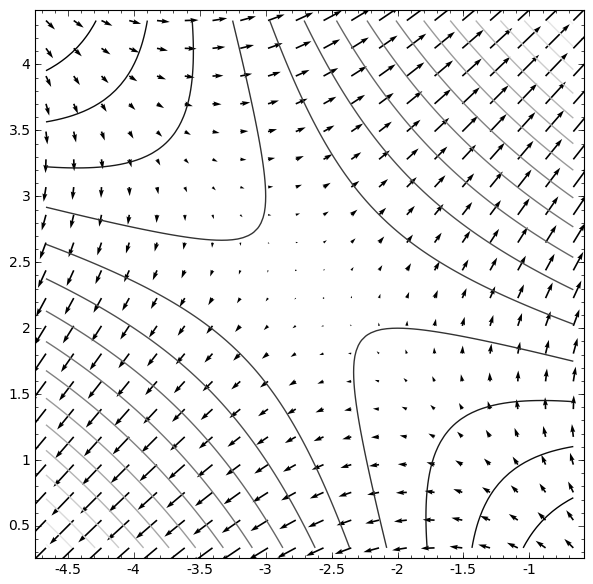
\includegraphics[width=\marginparwidth]{second-derivative-test.png}
}
 Consider the function $f(x,y)= x^2+4xy-4x+y^2+6y$. The derivative (gradient) is the vector field $Df(x,y) = (2x+4y-4,4x+2y+6)$. 
%See Figure \ref{second derivative graph} for a graph of several level curves, together with the gradient.
\begin{enumerate}
\item 
At what point(s) does $Df(x,y)=\vec 0$? These are the potential locations of maximums, minimums, or saddles.   
\item 
Compute the second derivative of $f$, which should give you a 2 by 2 symmetric matrix. This matrix is called the Hessian.
\item 
By looking at the plot to the right, are the eigenvalues of $D^2f(x,y)$ both positive, both negative, or do they differ in sign?  How can you tell? Then confirm you are correct by computing the eigenvalues and eigenvectors of $D^2f(x,y)$.  
\item 
Recall that the gradient points in the direction of greatest increase.  Using this information alone, does the function have a maximum, minimum, or saddle point.
\end{enumerate}

%\begin{figure}
% \begin{center}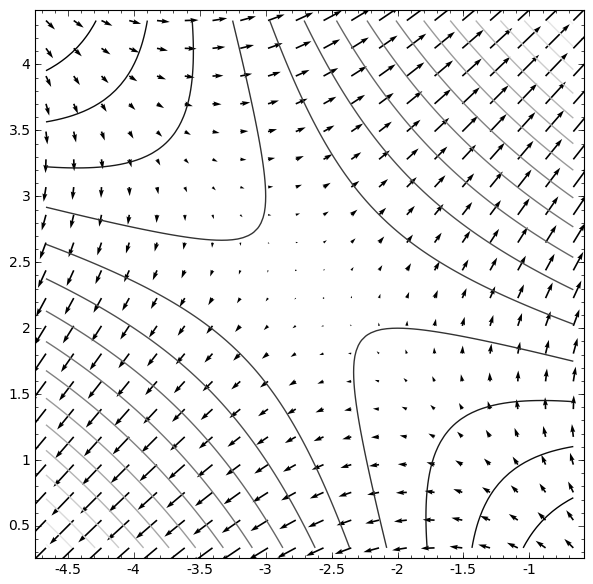
\includegraphics[width=\marginparwidth]{second-derivative-test.png}\end{center}
%\caption{A plot of several level curves of $f(x,y)=x^2+4xy-4x+y^2+6y$ and the gradient (the graph is not centered at the right spot, so ignore the axes). In one direction the gradient is pulling things towards the origin.  In another direction, the gradient is pushing things away from the origin. \label{second derivative graph}}
%\end{figure}
\end{problem}

We can summarize the results from the problem above into a theorem from multivariate calculus. 
\begin{theorem}
 Let $f(x,y)$ be a function that is twice continuously differentiable. Suppose that $Df(x,y)=(0,0)$ when $(x,y)=(a,b)$, so that $(a,b)$ is a critical point. To determine if the point $(a,b)$ corresponds to a maximum, minimum, or saddle point, we compute the eigenvalues of $D^2f(a,b)$ (the second derivative is called the Hessian).
\begin{itemize}
 \item If all eigenvalues are positive, then $f$ has a minimum at $(a,b)$. 
 \item If all eigenvalues are negative, then $f$ has a maximum at $(a,b)$. 
 \item If the eigenvalues differ in sign, then $f$ has a saddle at $(a,b)$. 
 \item If zero is an eigenvalue, then the second derivative test fails.
\end{itemize}
\end{theorem}



\mysubsection{\ideapro}

\begin{problem}
 Sally found the treasure in the corn field.  She's now looking for treasure in a swamp. There's a road through the swamp that runs parallel to the vector $\vec v=(3,4)$. Her current location is $(0,0)$ and the treasure (geocache) is located at the position $\vec b=(2,-4)$ (units are hundreds of yards). When Sally decides to leave the road, she'll have to wade through some swamp water. She would prefer to spend as little time in the swamp as possible. Her goal is to walk along the road until she reaches the point closest to the treasure, and then wade straight to the treasure.  This means she needs to find a scalar $c$ so that $c\vec v$ gets her as close to the treasure as possible. See the picture below. 
\begin{center}	
\begin{tikzpicture}[scale=1]
\draw[thin] (-3,-4) -- (3.3,4.4);
\draw [->,thick] (0,0) -- node [left=3pt]{$\vec v=(3,4)$}(3,4);
\draw [->,thick,red,dashed] (0,0) -- node [right=3pt]{$\vec b=(2,-4)$}(2,-4);
\draw [->,very thick,green] (0,0) -- node [left=3pt]{$c\vec v$}(-1.2,-1.6);
\draw [->,very thick,blue] (-1.2,-1.6) -- node [below=3pt]{$\vec n$}(2,-4);
\end{tikzpicture}
\quad 
\begin{tikzpicture}[scale=1]
\draw [->,thick] (0,0) -- node [left=3pt]{$\vec v$}(3,4);
\draw [->,thick] (0,0) -- node [right=3pt]{$\vec b=c\vec v+\vec n$}(2,-4);
\draw [->,thick] (0,0) -- node [left=3pt]{$c\vec v$}(-1.2,-1.6);
\draw [->,thick] (-1.2,-1.6) -- node [below=3pt]{$\vec n$}(2,-4);
\end{tikzpicture}
\end{center}
The vector $\vec n$ represents the path she must take through the swamp. Her goal is to find a scalar $c$ so that $\vec b=c\vec v+\vec n$ and $\vec n$ is as short as possible. 
\begin{enumerate}
 \item What is the angle between $\vec v$ and $\vec n$? Why does $\vec v\cdot \vec n=0$?
 \item Sally knows that the treasure is at $\vec b = c\vec v+\vec n$.  Since $\vec v\cdot \vec n = 0$, she decides to dot both sides of this equation, on the left, by the vector $\vec v$ to get $\vec v\cdot \vec b = \vec v\cdot (c\vec v+\vec n)$. Show that in general $$c = \dfrac{\vec v\cdot \vec b}{\vec v\cdot \vec v} 
%= \dfrac{\vec v^T\vec b}{\vec v^T\vec v}.
$$ Then show that with Sally's specific road vector $\vec v$ and treasure vector $\vec b$, the constant $c$ is $c=-2/5$. 
 \item We know that $c\vec v$ is as close to $\vec b$ as you can get along the road. Since $\vec b = c\vec v+\vec n$ and we know $c\vec v$, solve for $\vec n$. Then find the distance Sally will have to travel in the swamp (what's the length of $\vec n$)? 
\end{enumerate}
 \end{problem}
 
The vector $c\vec v$ above is often called the orthogonal projection of $\vec b$ onto $\vec v$. The word orthogonal means that $\vec v\cdot \vec n=0$, i.e. that there is a 90 degree angle between $\vec v$ and $\vec n$. 
%The scalar $c$ is sometimes called a Fourier coefficient.    


\begin{problem}
 Now assume that Sally is an astronaut in space. She's moving through an asteroid field and knows there is safe passage if she follows the vector $\vec v = (1,-2,-3)$. She needs to get to the point $\vec b=(3,-6,-11)$. She already knows that if she follows $\vec v$ three times, she'll end up pretty close by arriving at $(3,-6,-12)$. However, she wants to follow $\vec v$ until she is as close to $\vec b$ as possible, as leaving the known safe path could be dangerous.  
\begin{enumerate}
 \item 
Determine the scalar $c$ so that $\vec v c$ is as close to $\vec b$ as possible. Your answer should be close to 3.  Use the formula from the previous problem.
  \item 
Let's swap to a different question. 
Suppose we would like to find an equation of a line $y=mx$ through the origin that passes through the three points  $(1,3)$, $(-2,-6)$, and $(-3,-11)$.
To pass through all three points we need to solve the system of equations $3=m(1)$, $-6=m(-2)$, and $-11=m(-3)$. 
Rewrite this system of equations as the vector equation (state $\vec v$ and $\vec b$) 
$$\vec v m = \vec b \quad\quad\quad\Rightarrow\quad\quad\quad \bvec{?\\?\\?}m = \bvec{?\\?\\?}.$$
Explain why there is no solution to this problem. 
  \item
What should we choose the slope $m$ to equal so that $\vec v m$ will be as close to $\vec b$ as possible? [Hint: Multiply both sides on the left by the matrix $\vec v^T$.]
 \end{enumerate}
\end{problem}


\mysubsection{\ideacon}

Many problems in nature arise from conservation laws.  These laws generally focus on the principle that matter is neither created nor destroyed, rather it is just moved, changed, or something.  Any of the following could be viewed as a conservation law:
\begin{itemize}
 \item What comes in must come out.
 \item Voltage supplied equals voltage suppressed.
 \item Atoms before equal atoms after.
 \item The change in a quantity is how much it increases minus how much it decreases.
 \item Current in equals current out.
 \item The sum of the forces in every direction must match the total force.
 \item The force and moments must sum to zero when an object is at rest.
 \item This list could go on for a while.
\end{itemize}
Throughout this chapter, we'll see several different conservation laws.  You'll focus on understanding these conservation laws in your major classes. We'll see that almost every one of these problem can be written in the matrix form $A\vec x=\vec 0$. We'll see that $\lambda=0$ is an eigenvalue, which means that when we follow the eigenvector direction, the underlying vector field neither pushes outward nor inward. In this eigenvector direction, the system is conserving something.
\begin{definition}[Homogeneous System, Kernel]\label{homogeneous and kernel of a matrix}
Because we'll encounter problems of the form $A\vec x = \vec 0$ quite often, we make some definitions. 
\begin{itemize}
 \item We say that the linearly system $A\vec x=\vec b$ is homogeneous if $\vec b=\vec 0$. 
 \item The set of solutions to $A\vec x=\vec 0$ is called the kernel (or null space) of $A$.  
\end{itemize}
\end{definition}



Chemical reaction stoichiometry is the study of balancing chemical equations. A chemical reaction will often transform reactants into by-products. The by products are generally different compounds, together with either an increase or decrease in heat. One key rule in stoichiometry is that a chemical process neither creates nor destroys matter, rather it only changes the way the matter is organized. For simple reactions (with no radioactive decay), this conservation law forces the number of atoms entering a reaction to be the same as the number leaving. The next problem asks you to use this conservation law to create a balanced chemical reaction equation. 
\begin{problem}[Stoichiometry]
 The chemical compound hydrocarbon dodecane ($C_{12}H_{26}$) is used as a jet fuel surrogate (see Wikipedia for more info).  This compound reacts with oxygen $(O_2)$, and the chemical reaction produces carbon dioxide ($CO_2$), water ($H_2 O$), and heat.  Suppose we expose some dodecane to oxygen, and that a chemical reaction occurs in which the dodecane is completely converted to carbon dioxide and water.  
 Conservation requires that the number of atoms ($H$, $C$, and $O$) at the beginning of the chemical reaction must be the exact same as the number at the end. 
 We could write the chemical reaction in terms of molecules as
 $$x_1 C_{12}H_{26} +x_2 O_2 = x_3 CO_2+ x_4 H_2O\quad \text{or} \quad x_1 C_{12}H_{26} +x_2 O_2 - x_3 CO_2- x_4 H_2O=0, $$
 where $x_1$ molecules of dodecane and $x_2$ molecules of oxygen were converted to $x_3$ units of carbon dioxide and $x_4$ units of water.  
 If we look at each atom (carbon, hydrogen, and oxygen) individually, we obtain three equations to relate the variables $x_1, x_2, x_3, x_4$.  The carbon equation is simply
 $$x_1(12) + x_2(0) = x_3(1)+x_4(0) \quad \text{or}\quad x_1(12) + x_2(0) - x_3(1)-x_4(0)=0.$$  
 Your job follows:
\begin{enumerate}
 \item Write the other two conservation equations (for hydrogen and oxygen), and then organize your work into the matrix product $A\vec x = \vec 0$. This means you are working with a homogeneous system.
 \item Solve the corresponding system of equations by row reduction.  As there are only 3 equations with 4 unknowns, you should obtain infinitely many solutions. Write each variable in terms of the free variable.  You have found the kernel of the matrix $A$. 
 \item If about 10,000 molecules of water are present at the end of the reaction, about how many molecules of dodecane were burned? 
 \item 
\marginpar{If your answer on part 4 looks like your answer on the previous part, good. The point is that finding an eigenvector corresponding to $\lambda=0$ is the exact same as finding the kernel.}%
The matrix $A$ was not square.  We can make the system square by adding the trivial equation $0=0$, a row of zeros, to the bottom of the matrix. Let $B$ be this matrix. Why do we know $\lambda=0$ is an eigenvalue of this matrix?  Find an eigenvector corresponding to $\lambda=0$. 
\end{enumerate}
\end{problem}









\mysubsection{\idealin}


\begin{problem}\label{sally in city}
 After getting the treasure in the swamp, Sally moves on to find a treasure located in small town. She has a map of the town that shows the city blocks.  However, when she looks at a satellite image of the city it's slightly different than her map. Here are the two maps (the city map is on the left, the satellite on the right).
 \begin{center}
 \begin{tabular}{cc}
\begin{tikzpicture}
 \clip (0,0) circle (2.5cm);
 \draw[very thick] (0,0) circle (2.5cm);
 \foreach \x in {-3,-2,-1,0,1,2,3}
  \foreach \y in {-3,-2,-1,0,1,2,3}
   \draw[thick,blue] (\x,\y)--(\x+1,\y);
 \foreach \x in {-3,-2,-1,0,1,2,3}
  \foreach \y in {-3,-2,-1,0,1,2,3}
   \draw[thick,blue] (\x,\y)--(\x,\y+1);
 \fill (0,0) circle (.1cm);
 \end{tikzpicture}
&
 \begin{tikzpicture}[scale=.36]
 \clip (0,0) circle (7cm);
 \draw[very thick] (0,0) circle (7cm);
 \foreach \x in {-4,-3,-2,-1,0,1,2,3}
  \foreach \y in {-4,-3,-2,-1,0,1,2,3}
   \draw[thick,blue] (\x+2*\y,3*\x-\y)--(\x+1+2*\y,3*\x+3-\y);
 \foreach \x in {-4,-3,-2,-1,0,1,2,3}
  \foreach \y in {-4,-3,-2,-1,0,1,2,3}
   \draw[thick,blue] (\x+2*\y,3*\x-\y)--(\x+2*\y+2,3*\x-\y-1);  
 \fill (0,0) circle (.3cm);
%Eventually I would like to put the vectors in this problem. at nodes.  I don't know the syntax yet. 
%\draw node at (1,3) {$(0,0)$}
 \end{tikzpicture}
\\
City Map&Satellite View
 \end{tabular}
 \end{center}
 The city grid is not lined up with compass directions. When the city map tells her to go up one block, this really means her $(x,y)$ position should follow the vector $\vec v_1=(1,3)$. To go right 1 block, she follows the vector $\vec v_2=(2,-1)$. She has to learn to work with two different coordinate systems, namely the city coordinates (given in blocks) and the $(x,y)$ satellite coordinates (given in hundreds of yards). Assume that Sally is currently at the origin $(0,0)$. 
%She's currently standing at the point $A$ (which we'll consider the origin). Her GPS unit tells her that the treasure is located at the coordinates (). Our goal on this problem is to determine how she should follow the roads to get to the treasure.
\begin{enumerate}
 \item If Sally goes up 2 blocks, and right 3 blocks, what are here $(x,y)$ coordinates (in hundreds of yards)?
 \item If Sally moves up $c_1$ blocks and right $c_2$ blocks, then what are her $(x,y)$ coordinates. Write your answer as a linear combination of vectors, and then as a matrix product $A\bvec{c_1\\c_2}=\bvec{x\\y}$. You can check if you are correct by computing $A\bvec{1\\0}=\bvec{1\\3}$ and $A\bvec{0\\1}=\bvec{2\\-1}$. 
 \item If the treasure is located at the $(x,y)$ coordinates $(0,7)$, what directions would you give her in terms of blocks? If the treasure is located at $(1,-7.5)$, what directions would you give?
 \item What does the determinant of the matrix $A$ have to do with the maps?
\end{enumerate}

\end{problem}


One way we can use a matrix is to think of the matrix as a map. When Sally was walking through the city in Problem \ref{sally in city}, she had a map of the city in her hands.  This map gave her the coordinates of locations in the city, but did so in a much simplified way. Going right on the map 1 block resulted in following the vector $(2,-1)$.  Going up 1 block resulted in following the vector $(1,3)$. It's much easier to give directions in terms of blocks.  

If Sally walks 2 blocks right, and 1 block up, then she arrives at $\bvec{2\\-1}(2)+\bvec{1\\3}(1) = \bvec{7\\1}$. In the city map, we base our all movement on the vectors $(1,0)$ and $(0,1)$. When looking at actual $(x,y)$ position, we base all our movements on the vectors $(2,-1)$ and $(1,3)$. We call each of these collections of independent vectors a basis.  We call $(c_1,c_2)=(2,1)$ the coordinates of the point $(x,y)=(7,1)$ relative to the basis $\{(2,-1),(1,3)\}$. 
We can describe any point $(x,y)$ using the simplified coordinates $(c_1,c_2)$ relative to this basis.


\begin{definition}[Basis and Coordinates Relative to a Basis]
 If the vectors $\vec v_1, \vec v_2,\ldots,\vec v_n$ are linearly independent, then we'll say these vectors form a basis.  
 We use the word ``basis'' because we can write (base) other vectors uniquely as a linear combination of these basis vectors.  You have been using the standard basis vectors $(1,0)$ and $(0,1)$ your entire life to talk about vectors in the plane. To plot the point $(2,3)$, we think ``right 2, up 3'' which is the same as the vector equation $(2,3)=2(1,0)+3(0,1)$. 

 Suppose $\mathscr{B}=\{\vec v_1, \vec v_2, \ldots, \vec v_n\}$ is a basis, and $\vec x$ is the linear combination
 $$\vec x = \vec v_1c_1+\vec v_2c_2+\cdots +\vec v_n c_n.$$
 Then we call $c_1, c_2, \ldots,c_n$ the coordinates of $\vec x$ relative to the basis $\mathscr{B}$. 
 
 In terms of matrices, when the columns of $A$ are linearly independent and $A\vec c=\vec x$, we say that $\vec c$ is the  coordinates of $\vec x$ relative to the columns of $A$. 
\end{definition}

A matrix $A$ takes each coordinate $(c_1,c_2)$ and transforms it to the point $\bvec{x\\y}=A\bvec{c_1\\c_2}$. You'll see in the next problem that lines get transformed to lines. For this reason, and others we'll soon see,  we call this coordinate transformation map a linear transformation. 

\begin{problem}\label{candice's treasure}
 Consider the matrices $A=\bvec{\nvec{1\\2}&\nvec{-1\\4}}$ and $B=\bvec{\nvec{1\\2}&\nvec{3\\-2}}$.  
 \begin{enumerate}
  \item 
  Consider  
  $\bvec{\nvec{1\\2}&\nvec{-1\\4}&\nvec{-1\\10}&\nvec{3\\0}&\nvec{1\\2}&\nvec{1\\0}}
  \xrightarrow{rref}
  \bvec{\nvec{1\\0}&\nvec{0\\1}&\nvec{1\\2}&\nvec{2\\-1}&\nvec{1\\0}&\nvec{2/3\\-1/3}}
  $.
  
  If we want to write $(x,y)=(-1,10)$ as a linear combination of the columns of $A$, what scalars (coordinates) $c_1$ and $c_2$ give $\pvec{1\\2}c_1+\pvec{-1\\4}c_1=\pvec{-1\\10}$?
  
  What are the coordinates of $(x,y)=(3,0)$ relative to the columns of $A$?  

  What are the the coordinates of $(1,0)$ relative to the basis $\{(1,2), (-1,4)\}$?
  \item
 Alice decides to walk around using coordinates relative to the columns of $A$.  She starts at $(0,0)$, and then walks to the $(c_1,c_2)$ coordinates $(1,0)$, then $(1,2)$, then $(0,1)$, and then back to $(0,0)$. Her path in the $(x,y)$ plane is shown below on the right.  
 \begin{center}
\newcommand{\mux}{1}
\newcommand{\muy}{2}
\newcommand{\mvx}{-1}
\newcommand{\mvy}{4}
\begin{tikzpicture}
\node (A) at (0,0) {\begin{tikzpicture}
  axis
  \draw (-1,0) -- coordinate (x axis mid) (2,0);
  \draw (0,-1) -- coordinate (y axis mid) (0,3);
  ticks
  \foreach \x in {-1,...,2}
   \draw (\x,1pt) -- (\x,-3pt)
    node[anchor=north] {};
  \foreach \y in {-1,...,3}
   \draw (1pt,\y) -- (-3pt,\y) 
    node[anchor=east] {}; 
  \fill[opacity=.2] (0,0) -- (1,0) -- (1,2) -- (0,1) -- (0,0);
  \draw[red,->,very thick] (0,0)--(1,0);
  \draw[blue,->,very thick] (0,0)--(0,1);
  \node at (.5,-1.5) {Coordinates $(c_1,c_2)$};
\end{tikzpicture}};
\node[right=of A ] (B) {\begin{tikzpicture}[scale=.5]
  axis
  \draw (-2,0) -- coordinate (x axis mid) (2,0);
  \draw (0,-1) -- coordinate (y axis mid) (0,10);
  ticks
  \foreach \x in {-2,...,2}
   \draw (\x,1pt) -- (\x,-3pt)
    node[anchor=north] {};
  \foreach \y in {-1,...,10}
   \draw (1pt,\y) -- (-3pt,\y) 
    node[anchor=east] {}; 
  \fill[opacity=.2] (0,0) -- (\mux,\muy) -- (\mux+2*\mvx,\muy+2*\mvy) -- (\mvx,\mvy) -- (0,0);
  \draw[red,->,very thick] (0,0)--(\mux,\muy);
  \draw[blue,->,very thick] (0,0)--(\mvx,\mvy);
  \node at (-2,-1.5) {Position $(x,y)$};
 \end{tikzpicture}};
 \draw[->] (A.east) -- node[above=3pt]{\footnotesize $A\bvec{c_1\\c_2} = \bvec{x\\y}$} (B.west);
\end{tikzpicture}
\end{center}
Bob decides to follow the same coordinate path, but he's using coordinates relative to the columns of $B$.  Draw Bob's path in the $(x,y)$ plane.  Remember that since we know coordinates $(c_1,c_2)$, we can get the $(x,y)$ position from $B\bvec{c_1\\c_2}=\bvec{x\\y}$. 

 
 %(How can you tell that Bob got his map by taking a picture of someone else map in a mirror?)
%I chose a bad matrix, because you loose the entire point to this problem.  It looks bad when you graph it, because something lines up perfectly. 
  \item 
 Candice is staring at a treasure map.  She doesn't have a matrix $C$ to help her translate from the treasure map to actual $(x,y)$ points. However, she does have a few bits of information. There are two trees on her map with coordinates $(c_1,c_2)$ at $(2,1)$ and $(-4,-3)$. The actual $(x,y)$ location of these trees is $(-4,5)$ and $(7,-10)$  This means if Candice knew $C$, then she could compute $C\bvec{\nvec{2\\1}}=\bvec{\nvec{-4\\5}}$ and $C\bvec{\nvec{-4\\-3}}=\bvec{\nvec{7\\-10}}$.  Combining these two products together into one matrix means $$C\bvec{\nvec{2\\1}&\nvec{-4\\-3}}=\bvec{\nvec{-4\\5}&\nvec{7\\-10}}.$$  Use this to find $C$.  [Hint: Try using an inverse matrix.]
 \item The treasure on Candice's map has the map coordinates $(-1,5)$.  Give Candice the $(x,y)$ location of the treasure.   
 \end{enumerate}

\end{problem}







%7










%7 - Adjoint Problem


\begin{problem}
Consider the matrix
$A=\begin{bmatrix}
2&1&-1\\1&2&0\\0&4&3 
\end{bmatrix}.$
\begin{enumerate}
 \item 
 Compute the determinant of $A$. 
 \item 
\marginpar{If you forgot what a cofactor is, you'll want to review the definition.  See Definition \ref{general determinants} on page \pageref{general determinants}. }%
Now create a matrix $B$ so that the $ij$th entry of $B$ is the cofactor $C_{ij}$ (remove row $i$ and column $j$, compute the determinant, and then times by an appropriate sign).  
This will require that you compute nine 2 by 2 determinants.  
 \item 
Compute the inverse of $A$ with software. 
 \item 
Make a conjecture about the connection between the determinant of $A$, this matrix of cofactors $B$, and the inverse of $A$.  
\end{enumerate}
%We'll verify your conjecture is true on a 4 by 4 matrix in class. 
\end{problem}


In your work above, you should have noticed that you had to reverse the rows and columns of $B$ to make your conjecture.  This process of reversing rows and columns, called transposing a matrix, will show up in so many of our applications that we make a definition.

\begin{definition}[The Transpose $A^T$. Symmetric Matrix]
 If $A$ is an $m$ by $n$ matrix, then the transpose of $A$ is the $n$ by $m$ matrix formed by interchanging the rows and columns.  Row 1 is now column 1. Row 2 is now column 2.  Just think of each row as a vector, and then place those vectors in the columns of a new matrix.  We use the symbol $A^T$ to stand for the transpose of a matrix.

We'll often encounter square matrices where the transpose of the matrix is the matrix itself.  If $A=A^T$ then we say the matrix is symmetric. When a vector field has a potential, its derivative satisfies this property. 
\end{definition}









%8
\begin{problem}
\marginpar{
For the matrix $A=\bvec{2&1\\0&3}$, you should see the two pictures below.

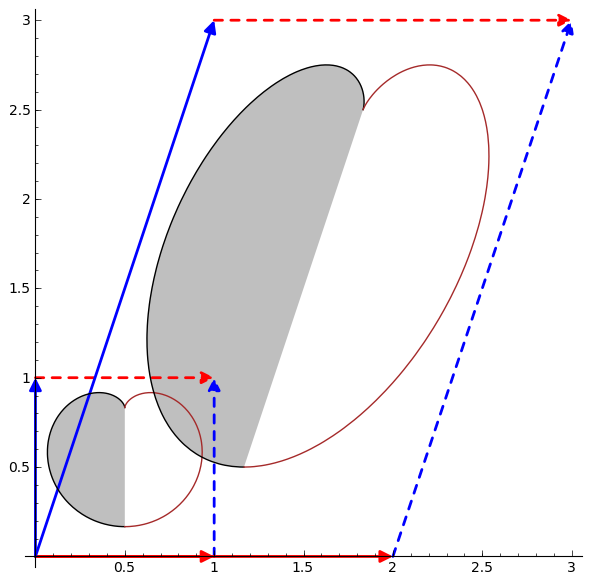
\includegraphics[width=\marginparwidth]{lineartransformation1.png}

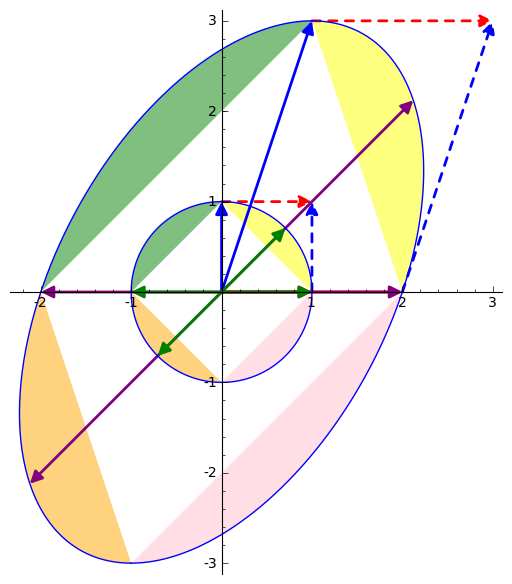
\includegraphics[width=\marginparwidth]{lineartransformation2.png}
}%
 On this problem, you will explore graphs of several linear transformations. Your job is to look for patterns and explanations.  Please head to the following webpage:
\begin{itemize}
 \item \href{\urllineartransformationsinplane}{\urllineartransformationsinplane}
\end{itemize}
You may find this problem easiest if you create your own account at sagemath.org, and then copy the code from the URL above to your own notebook. Then you can put 10+ linear transformation graphs in the same document so you can compare them all side by side. 

Here's your job. In the software link above, change the matrix $A$ to be several different matrices. Look for an answer to each question below.
\begin{itemize}
 \item What does the determinant tell you about the map? Can you see the determinant in the pictures?
 \item If the determinant is zero, what does that mean about your map?
 \item What do the eigenvalues tell you about your map? This is perhaps easiest to tell with the circle map.
 \item Is there a connection between the eigenvalues and the determinant?
 \item What do the eigenvectors tell you?
 \item Does anything special happen if the matrix is symmetric?
\end{itemize}
To be prepared for class, write answers to these questions using complete sentences.
There are many great answers to the questions above. There are lots of patterns. 

Here are some matrices that might be useful to look at. Please type each of these in.  As you discover patterns, test them against these matrices. 
$$
\bvec{2&1\\0&3},
\bvec{-2&1\\0&3},
\bvec{-2&1\\0&-3},
\bvec{0&4\\3&1},
\bvec{2&1\\1&2},
\bvec{1&2\\2&4},
\bvec{0&-1\\1&0},
\bvec{-1&2\\2&1},
$$
$$\bvec{\cos(pi/3)&-\sin(pi/3)\\ \sin(pi/3)&\cos(pi/3)},
\bvec{3\cos(pi/6)&-5\sin(pi/6)\\ 3\sin(pi/6)&5\cos(pi/6)}.
$$
\end{problem}
%end 8

















%9
\mysubsection{\ideanon}
\begin{problem}
\marginpar{
Here's a plot of several level curves of $f(x,y)=x^3-3x^2-y^2+2y$ and the gradient. There are two critical points.  

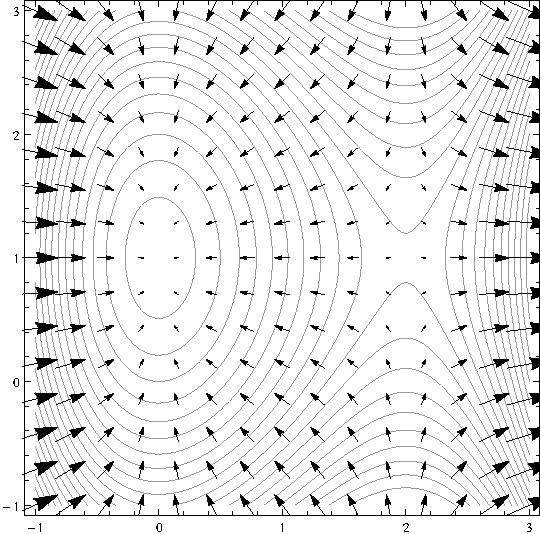
\includegraphics[width=\marginparwidth]{second-derivative-test2}
}%
 Consider the function $f(x,y) = x^3 - 3x ^2 - y^2 + 2y$
\begin{enumerate}
\item 
At what point(s) does $Df(x,y)=\vec 0$? You should obtain two points. These are the potential locations of maximums, minimums, or saddles.   
 \item 
Compute the second derivative of $f$, which is a 2 by 2 symmetric matrix. 
 \item 
Pick one of the critical points. Use the vector field plot to the right to decide if the eigenvalues of $D^2f(x,y)$ are both positive, both negative, or differ in sign at that critical point. Then state if the function has a maximum, minimum, or saddle at that point.  Then repeat with the other critical point. 
 \item 
Now compute the eigenvalues of the Hessian at each critical value. You'll need to find the eigenvalues of two different matrices.  This should confirm your answer to part 3. (The matrix is diagonal, so computing eigenvalues should be quick.)  
Don't forget that you are finding eigenvalues of $D^2f(a,b)$, not $D^2f(x,y)$. 
\end{enumerate}
\end{problem}


The following example adds a little more information to this discussion. I've included it to give you one additional piece of information, namely how the eigenvalues and eigenvectors connect to the concavity of the function. 

\begin{example}
For the function {$f(x,y)=x^2+xy+y^2$}, the gradient is $Df = \begin{bmatrix}2x+y&x+2y \end{bmatrix}$, which is zero only at $x=0,y=0$ (solve the system of equations $2x+y=0,x+2y=0$). The Hessian is $D^2f = \begin{bmatrix}2&1 \\1&2\end{bmatrix}$. The eigenvalues are found by solving $0=\det \begin{bmatrix}2-\lambda &1 \\1&2-\lambda \end{bmatrix} = (2-\lambda)^2-1 = 4-4\lambda+\lambda^2 -1 = (\lambda-3)(\lambda-1)$, so $\lambda = 3,1$ are the eigenvalues.  Since both eigenvalues are positive, the gradient pushes things away from the origin in all direction, which means in every direction you move from the critical point, you'll increase in height.  There is a minimum at $(0,0)$.  

The eigenvectors of the Hessian help us understand more about the graph of the function.  An eigenvector corresponding to 3 is $(1,1)$, and corresponding to 1 is $(-1,1)$. These vectors are drawn in figure \ref{2ndder}, together with two parabolas whose 2nd derivatives are precisely 3 and 1.  The parabola which opens upwards the most quickly has a 2nd derivative of 3.  The other parabola has a second derivative of 1. In every other direction, the 2nd derivative would be between 1 and 3.
\end{example}

%\marginpar{{
\begin{figure}[ht
]\begin{center}
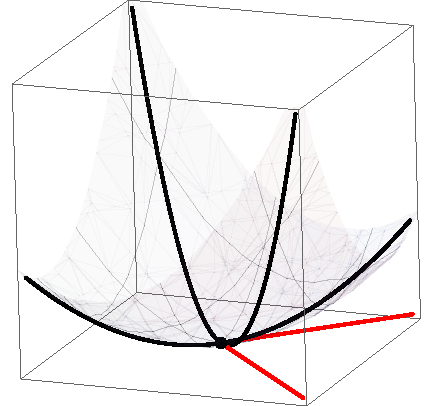
\includegraphics[width=2in]{support/2nddertest1}
\hspace{.5in}
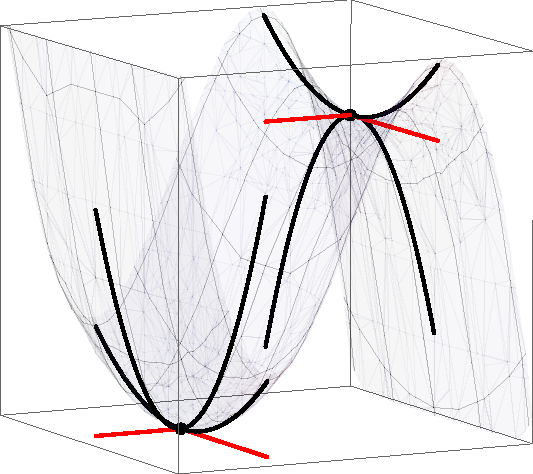
\includegraphics[width=2in]{support/2nddertest2}
\end{center}
\caption{The eigenvectors of the second derivative tell you the directions in which the 2nd derivative is largest and smallest. At each critical point, two eigenvectors are drawn as well as a parabola whose second derivative (the eigenvalue) matches the second derivative of the surface in the corresponding eigenvector direction.}
\label{2ndder}
\end{figure}
%}}
%end 9
















%10
\mysubsection{\ideapro}
\begin{problem}
Jimmy is using a rocket suit to travel out in space. His rocket suit had 4 good boosters that allowed travel in any direction, with a backup booster in case one got damaged.  However, some tiny meteorites happened to pass by and take out two of his boosters, as well as his radio to call for help.  He's now only able to move in the directions $\vec v_1=(1,1,1)$ and $\vec v_2=(-1,1,2)$.  His space ship is sitting at $\vec b=(-1,4,7)$.
\begin{enumerate}
 \item 
 Show that Jimmy cannot arrive at his ship using his two working boosters.  In other words, show that we cannot write $\vec b$ as a linear combination of $\vec v_1$ and $\vec v_2$? Set up an appropriate matrix equation, row reduce the equation, and use your row reduction to give an answer. 
 \item 
 Jimmy has a one shot back up gun.  This gun will propel him towards the ship if he points the gun directly away from the ship and fires.  
 It's easy to miss aim, so he would like to get as close to the ship as possible before he fires the gun. 
 He needs to find $c_1$ and $c_2$ so that $\vec w = \vec v_1 c_1+\vec v_2 c_2$ gets him as close to the ship as possible. The picture below illustrates the general idea. The vectors $\vec v_1$ and $\vec v_2$ give Jimmy a plane of possible movements. 
\begin{center}	
\begin{tikzpicture}[scale=1]
\fill[lightgray] (0,0) -- (-2,2) -- (2,2) -- (4,0) -- (0,0);
\draw[thin] (-1,0) -- (4,0);
\draw[thin] (.5,-.5) -- (-2,2);
\draw [->,thick] (0,0) -- node [below=3pt]{$\vec v_1$}(3,0);
\draw [->,thick] (0,0) -- node [left=3pt]{$\vec v_2$}(-1,1);
\draw [->,thick] (0,0) -- node [left=3pt]{$\vec b$}(2,4) node[right=3pt]{The space ship is up here.};
\draw [->,thick] (0,0) -- node [right=3pt]{$\vec w = \vec v_1 c_1+\vec v_2 c_2$}(2,2) node[right=3pt]{Jimmy wants to get here.};
\draw [->,thick] (2,2) -- node [right=3pt]{$\vec n$}(2,4);

%\draw [->,thick] (-1.2,-1.6) -- node [below=3pt]{$\vec n$}(2,-4);
\end{tikzpicture}
\end{center}
 When Jimmy has arrived at the closest spot to the ship, he'll have the smallest $\vec n$ so that 
$$\vec v_1 c_1+\vec v_2 c_2+\vec n=\vec b\quad\quad\text{ or }
\quad \quad 
\pvec{1\\1\\1} c_1+\pvec{-1\\1\\2} c_2+\vec n=\pvec{-1\\4\\7}.$$ Why must $\vec v_1^T\vec n=0$ and $\vec v_2^T\vec n=0$?  
 \item 
 Since there are two unknown constants $c_1$ and $c_2$, we need two equations.  Multiply both sides of the above equation on the left by $\vec v_1^T=\bvec{1&1&1}$. Why does $\vec n$ vanish from the equation? This gets us one equation.
 \item 
 To get a second equation, we multiply both sides by $\vec v_2^T=\bvec{-1&1&2}$. We now have two equations with two unknowns $c_1$ and $c_2$. Solve and show that $c_1 = 11/7$ and $c_2=37/14$.
% \item 
% Let $A =\bvec{\vec v_1&\vec v_2} = \bvec{1&-1\\1&2\\1&2}$. What does $A^TA$ and $A^T$ 
% You can organize all your work above into a single equation. Show that solving $A^TA\vec x = A^T\vec b$ for $\vec x$. 
\end{enumerate}

\end{problem}

The problem above asked you to find the point in a plane that was closest to a point not on the plane.  This is called the orthogonal projection of $\vec b$ onto the plane formed by the vectors $\vec v_1$ and $\vec v_2$.  If we let $A=\bvec{\vec v_1&\vec v_2}$, then the projection of $\vec b$ onto this plane is $w=\vec v_1c_2+\vec v_2c_2=A\bvec{c_1\\c_2}$. Our goal is to find $\bvec{c_1\\c_2}$ such that $\vec n=\vec b-A\bvec{c_1\\c_2}$ is as short as possible. The next problem shows that you can accomplish this by solving $A^TA\vec x=A^T\vec b$ for $\vec x$. We just take the problem $A\vec x=\vec b$ which has no solution, multiply both sides by $A^T$, and then solve.  
%end 10




 
 
 



%11
\begin{problem}
 Suppose we would like to find an equation of a line $y=a_0+a_1x$ that passes through the three points 
 $(-1,-1)$, $(1,4)$ and $(2,7)$. If such a line does not exist, we'd like to find a line that passes close to these three points. 
 \begin{enumerate}
  \item The three points give us three equations that involve the unknown constants $a_0$ and $a_1$. Show that we can write these equations in the matrix form $A\vec x = \vec b$ and vector form $\vec v_1a_0+\vec v_2a_1 = \vec b$ 
  $$\bvec{1&-1\\1&1\\1&2}\bvec{a_0\\a_1}=\bvec{-1\\4\\7}\quad\quad\text{or}\quad\quad \bvec{1\\1\\1}a_0+\bvec{-1\\1\\2}a_1=\bvec{-1\\4\\7}.$$
  Then show that there is no solution to this problem.
  \item We now know that no linear combination of $\vec v_1=(1,1,1)$ and $\vec v_2 =(-1,1,2)$ will give us the vector $\vec b=(-1,4,7)$.  We would like to find scalars $a_0$ and $a_1$ so that $\vec v_1a_1+\vec v_2a_1$ is as close to $\vec b$ as possible. This is the exact same question as the previous problem (where Jimmy could not get to his space ship). 
  Multiply both sides of the inconsistent equation $A\vec x = \vec b$ on the left by $\bvec{1\\1\\1}^T = \bvec{1&1&1}$, and then multiply both sides by  $\bvec{-1\\1\\2}^T = \bvec{-1&1&2}$. This should get you two different equations that involve $c_1$ and $c_2$. 
  \item Compute $A^TA = \bvec{1&1&1\\-1&1&2}\bvec{1&-1\\1&1\\1&2}$ and $A^T\vec b=\bvec{1&1&1\\-1&1&2}\bvec{-1\\4\\7}$.  You should see that both of your equations above are in the matrix equation  
  $$A^TA\vec x=A^T\vec b \quad \Rightarrow \quad \bvec{1&1&1\\-1&1&2}\bvec{1&-1\\1&1\\1&2}\bvec{a_0\\a_1}=\bvec{1&1&1\\-1&1&2}\bvec{-1\\4\\7}.$$ 
Make sure you simplify the matrix products $A^TA$ and $A^T\vec b$, as this should become a system of 2 equations and 2 unknowns. 
  \item Now solve $A^TA\vec x = A^T\vec b$ for $\vec x = \bvec{a_0\\a_1}$. Use your answer to state the line  $y=a_0 +a_1x$ that passes nearest these three points. 
 \end{enumerate}
\end{problem}
 
 The transpose of a matrix plays a crucial role in finding projections. When the problem $A\vec x =\vec b$ has no solution, it is impossible to write $\vec b$ as a linear combination of the columns of $A$.  If we multiply both sides on the left by $A^T$, then we have an equation that we can solve to obtain the coefficients $\vec x$ so that $A\vec x$ is as close to $\vec b$ as possible. This is the key idea to regression. 
%end 11







 
 
 


\mysubsection{\ideacon}
% 12
When we perform a partial fraction decomposition, Our goal is to rewrite a complicated fraction as the sum of simpler fractions.  We are not changing the quantity that the fraction represents, rather we are just changing how we express the fractions.  This is a conservations law, as the fractional quantity is conserved.  Can we answer this problem by looking for the kernel of some matrix, or an eigenvector corresponding to $\lambda=0$?

\begin{problem}\label{partial fraction general solution}
Consider the partial fraction decomposition 
$$
\frac{8s+7}{(s-2)(s+3)} = \frac{A}{s-2}+\frac{B}{s+3}
$$
which we  can rewrite in the form
$$8s+7 = A(s+3)+B(s-2).$$
Let's compare several different ways of solving this problem.
\begin{enumerate}
 \item Complete this partial fraction decomposition. Use any method you like. 
 \item Now let's solve 
$$
\frac{cs+d}{(s-2)(s+3)} = \frac{A}{s-2}+\frac{B}{s+3}
$$
Rather than thinking of $c$ and $d$ as known constants, let's make them variables in our linear system of equations.  
Our goal is to solve 
$$
(A+B-c)s+(3A-2B-d)=0
$$   
which we can rewrite in the matrix form 
\marginpar{Why did I save the last two columns for $c$ and $d$?}%
$$\bvec{
1 & 1 & -1 & 0 \\
3 & -2 & 0 & -1
}\bvec{A\\B\\c\\d}=\bvec{0\\0}.$$
This is a matrix equation of the form $A\vec x=\vec 0$, so the solutions are the kernel of $A$. Solve this matrix equation (find the kernel of $A$) and write your answer in terms of the free variables. Please use software to row reduce, and just share the key parts of your work (as shown below).
$$\bvec{[cccc|c]*&*&*&*&*\\ *&*&*&*&*}\xrightarrow{\text{rref}}\bvec{[cccc|c]1&0&*&*&*\\ 0&1& *&*&*}\Rightarrow \pvec{A\\B\\c\\d}=\bvec{*\\ *\\ *\\ * }c+\bvec{*\\ *\\ *\\ * }d.$$

\item 
We can rewrite the two equations $c=c$ and $d=d$ as the equations $0=0$ and $0=0$. Adding two rows of zeros to our matrix equation yields
$$\bvec{
1 & 1 & -1& 0 \\
3 &-2 & 0 & -1\\
0 & 0 & 0 & 0\\
0 & 0 & 0 & 0
}\bvec{A\\B\\c\\d}=\bvec{0\\0\\0\\0}.$$
Can you explain, from the definition of eigenvalues, why $\lambda =0$ is an eigenvalue of this matrix? Then find all eigenvectors of this matrix corresponding to $\lambda=0$.

\item 
Change the 4 by 4 matrix above to solve the partial fraction decomposition
$$
\frac{cs+d}{(s-p)(s-q)} = \frac{A}{s-p}+\frac{B}{s-q}.
$$
Then use software to solve, giving $A$ and $B$ in terms of $c,d,p,q$. %Under what conditions will your solution fail?
\end{enumerate}
\end{problem}
%end 12









% 13
%Traffic flow application
\begin{problem}[Traffic Flow]
Consider the following traffic flow grid.
\begin{center}
\begin{tikzpicture}[scale=1.3]
\begin{scope}[very thick, every node/.style={sloped,allow upside down}]
%\draw[step=1cm,gray,very thin] (-2,-2) grid (2,2);
\draw (-2,1)-- node(A) {\midarrow} (-1,1); 
\draw (-1,2)-- node(B) {\midarrow} (-1,1);  
\draw (1,1)-- node(C) {\midarrow} (1,2) ;  
\draw (1,1)-- node(D) {\midarrow} (2,1) ;  
\draw (2,-1) -- node(E) {\midarrow} (1,-1) ;  
\draw (1,-2) -- node(F) {\midarrow} (1,-1) ;  
\draw (-1,-1) -- node(G) {\midarrow} (-1,-2) ;  
\draw (-1,-1) -- node(H) {\midarrow} (-2,-1) ;  
\draw (-1,1) -- node(I) {\midarrow} (1,1) ;  
\draw (-1,1) -- node(J) {\midarrow} (-1,-1) ;  
\draw (1,-1) -- node(K) {\midarrow} (1,1) ;  
\draw (1,-1) -- node(L) {\midarrow} (-1,-1) ;  
\end{scope}
\draw (-1,1)  ++(-.2,.2) node {$A$}; 
\draw (1,1)  ++(-.2,.2) node {$B$}; 
\draw (1,-1)  ++(-.2,.2) node {$C$}; 
\draw (-1,-1)  ++(-.2,.2) node {$D$}; 
\node[left of=A] {100};
\node[above of=B] {200};
\node[above of=C] {100};
\node[right of=D] {150};
\node[right of=E] {50};
\node[below of=F] {50};
\node[below of=G] {50};
\node[left of=H] {100};
\node[label=above:$x_1$] at (I){};
\node[label=right:$x_2$] at (K){};
\node[label=below:$x_3$] at (L){};
\node[label=left:$x_4$] at (J){};
\end{tikzpicture}
\end{center}
The numbers on the edges represent the number of vehicles that either enter or leave the system each hour.  The variables $x_1$, $x_2$, $x_3$, and $x_4$ represent the number of cars on each road. Assume that all streets are one-way streets where the arrows give the direction of traffic flow.
\begin{enumerate}
 \item How do you know there are 400 total cars entering this network of roads each hour? Are all these cars leaving? Why is this a conservation problem?
 \item The number of cars entering an intersection must match the number of cars leaving an intersection.  We can use this to build a system of equations for the traffic flows $x_1, x_2,x_3, x_4$.  Every hour at node $A$ there are 300 cars entering the intersection and $x_1+x_4$ cars leaving the intersection. This gives us an equation $x_1+x_4=300$. Continue in this fashion to obtain an equation at each intersection point. You should have a system of 4 equations with 4 unknowns.
 \item 
Write your system of equations in the matrix form $A\vec x = \vec b$. What is $A$, what is $\vec x$, and what is $\vec b$? Is this system homogeneous or non homogeneous? 
 \item Solve your system of equations.  When you are presenting this kind of information in class, you should use the pattern $B\xrightarrow{\text{rref}}R\Rightarrow\vec x = ...$, so show us the augmented matrix $B$, show us its rref $R$, and then state the solution $\vec x$ as a linear combination of vectors, namely
$$
\bvec{[cccc|c]*&*&*&*&*\\ *&*&*&*&*\\ *&*&*&*&*\\ *&*&*&*&*}
\xrightarrow{\text{rref}}\bvec{[cccc|c]1&0&0&*&*\\ 0&1&0&*&*\\ 0&0&1&*&*\\ 0&0&0&0&0}\Rightarrow \pvec{x_1\\x_2\\x_3\\x_4}=\bvec{*\\ *\\ *\\ * }x_4+\bvec{*\\ *\\ *\\ * }.$$

 \item What's the minimum number and maximum number of cars that can be on the road $AD$ each hour? Explain.
\end{enumerate}
\end{problem}

Whenever I see a problem that involves a conservation law, I think two things. For one, there is probably a homogeneous system $A\vec x = \vec 0$ somewhere in the background whose kernel is the solution. Two, if I make sure $A$ is a square matrix (possibly adding rows of zeros), then I can rephrase ``find the kernel'' as ``find the eigenvectors corresponding to zero.'' To accomplish finding this matrix $A$, we'll often have to think of given constants as variables.  Let's do this with the previous problem. 

\begin{problem}
Use the same setting as the previous traffic flow problem, however, let's change the given values to be variables.  Starting in the upper left corner and moving clockwise, replace the numbers 100, 200, 100, 150, etc., with the variables $a$, $b$, $c$, $d$, $e$, $f$, $g$, $h$. We now have 12 unknowns, namely $x_1$, ..., $x_4$, $a$, $b$, ..., $h$. 
\begin{enumerate}
 \item  At node $A$, our equation is now $x_1+x_4-a-b=0$. Write the other 3 equations and express the homogeneous system in the form $A\vec x = \vec 0$ where $A$ is a 4 by 12 matrix.  State the matrix $A$.
 \item Find the kernel of $A$, and write your solution as a linear combination of vectors where the scalars are the free variables (use the $B\xrightarrow{\text{rref}}R\Rightarrow\vec x = ...$ pattern). Your solution should look like 
$$
\bvec{x_1\\ x_2 \\ x_3\\ x_4\\a\\b\\c\\d\\e\\f\\g\\h}=
\bvec{*\\ *\\ *\\ *\\ *\\ *\\ *\\ *\\ *\\ *\\ *\\ *}x_4+
\bvec{*\\ *\\ *\\ *\\ *\\ *\\ *\\ *\\ *\\ *\\ *\\ *}b+
\bvec{*\\ *\\ *\\ *\\ *\\ *\\ *\\ *\\ *\\ *\\ *\\ *}c+
\bvec{*\\ *\\ *\\ *\\ *\\ *\\ *\\ *\\ *\\ *\\ *\\ *}d+
\bvec{*\\ *\\ *\\ *\\ *\\ *\\ *\\ *\\ *\\ *\\ *\\ *}e+
\bvec{*\\ *\\ *\\ *\\ *\\ *\\ *\\ *\\ *\\ *\\ *\\ *}f+
\bvec{*\\ *\\ *\\ *\\ *\\ *\\ *\\ *\\ *\\ *\\ *\\ *}g+
\bvec{*\\ *\\ *\\ *\\ *\\ *\\ *\\ *\\ *\\ *\\ *\\ *}h.
$$ 
%\item Rewrite your solution, ignoring the rows corresponding to the free variables. Your answer should look like
%$$
%\bvec{x_1\\ x_2 \\ x_3\\a}=
%\bvec{*\\ *\\ *\\ *}x_4+
%\bvec{*\\ *\\ *\\ *}b+
%\bvec{*\\ *\\ *\\ *}c+
%\bvec{*\\ *\\ *\\ *}d+
%\bvec{*\\ *\\ *\\ *}e+
%\bvec{*\\ *\\ *\\ *}f+
%\bvec{*\\ *\\ *\\ *}g+
%\bvec{*\\ *\\ *\\ *}h.
%$$ 
\item 
The 4th row of your rref is not zero (which is why $a$ is not a free variable).  
Write the equation given by this 4th row.  Can you interpret this 4th equation as a conservation law?
\end{enumerate}
\end{problem}
%end 13









\mysubsection{\idealin}

Have you noticed in every matrix problem we can always write the solution as a linear combination of vectors? 
When the system is homogeneous, the solution to $A\vec x = \vec 0$ (the kernel) is always all linear combinations of a few vectors. We take a vector times a free variable, plus a vector times a free variables, etc. The solution is the set of all linear combinations of a few vectors. It would be nice to say ``all linear combinations of'' in an efficient way. We'll use the word span to talk about forming all linear combinations, the word vector space to talk about the vectors in the span, and then dimension to talk about the geometric size of the span (is it a line, a plane, a 3D space, etc.).

\begin{definition}[Span, Basis, Vector Space, and Dimension]\label{definition span, vector space, dimension}
Consider the set of vectors $S = \{\vec v_1,\vec v_2,\cdots, \vec v_n\}$. 
\begin{itemize}
 \item  
The span of $S$ is the set of all linear combinations of the vectors in $S$. 
 \item 
When the vectors in $S$ are linearly independent, we say that the vectors form a basis for their span.   
 \item 
A vector space is the span of a collection of objects (we'll focus on vectors and functions).  
 \item 
A basis for a vector space is a collection of linearly independent objects whose span is the vector space. 
 \item 
The dimension of a vector space is the number of vectors in a basis for the vector space.
\end{itemize}
\end{definition}




%15
\begin{problem}
We've seen each of the following problems before. On this problem, you'll practice using the words span, vector space, basis, and dimension. 
\begin{enumerate}
 \item In problem \ref{sally in corn field with 2 directions} on page \pageref{sally in corn field with 2 directions},  Sally could move along the road $(-1,1)$ and the rows of corn $(2,1)$. Is the span of these two vectors the entire plane? [Hint: You can row reduce $\bvec{[cc|c]-1&2&x\\1&1&y}$, or you can come up with another explanation as to why any vector $(x,y)$ must be a linear combination of the given two.] 
 \item Suppose our astronaut Jimmy has 4 boosters (see Problem \ref{rocket booster problem}) that allow bidirectional movement in the directions $(1,1,2)$, $(0,1,3)$, $(2,1,1)$, and $(-2,1,0)$. Show that the span of these vectors is all of three dimensional space. Then select from these boosters a basis for $\mathbb{R}^3$. [You'll want to row reduce a matrix to answer this. Show the matrix and its rref.]
 \item If the 4th booster breaks, what kind of object is the span of the remaining three directions? Is it all of space, a plane, a line, a circle, a parallelogram, etc.?  Then state the dimension of and give a basis for the vector space obtained as the span of these three vectors.
\end{enumerate}
\end{problem}
%end 15

The set of vectors $(x,y)$ in the plane forms a vector space of dimension 2.  We know this because the vectors $(1,0)$ and $(0,1)$ are linearly independent and we can obtain any point $(x,y)$ in the plane as the linear combination $(1,0)x+(0,1)y$. This shows that the two vectors $(1,0)$ and $(0,1)$ form a basis for the set of vectors in the plane. We call this vector space $\mathbb{R}^2$.  

\begin{problem}
Read the preceding paragraph (if you have not already). For each vector space below, produce a collection of independent vectors (or functions) whose span is the space. You might need to rref a matrix and obtain a solution first. State the dimension of the vector space. 
\begin{enumerate}
 \item The set of vectors $(x,y,z)$ in space ($\mathbb{R}^3$). 
 \item \marginpar{Your work here generalizes to show that the kernel of any matrix is always a vector space.}% 
 The kernel of the matrix 
$A=\bvec{
1 & 1 & -1 & 0 \\
3 & -2 & 0 & -1
}$ from Problem \ref{partial fraction general solution}. 
 \item 
 The solutions to $B\vec x = 3\vec x$ for 
$
B=
\begin{bmatrix}
 3 & 0 & 0 \\
 0 & 2 & 1 \\
 0 & 1 & 2
\end{bmatrix}
$ from Problem \ref{First example of deficient eigenvalue}.
\item The solutions to $C\vec x = 3\vec x$ for  
$
C=
\begin{bmatrix}
 3 & 1 & 0 \\
 0 & 2 & 1 \\
 0 & 1 & 2
\end{bmatrix}
$ from Problem \ref{First example of deficient eigenvalue}.
\item (Challenge) All polynomials $a_0+a_1x+a_2x^2+a_3x^3$ of degree 3 or less. 
\end{enumerate}
You can present in class if you got the first four. 
\end{problem}


From the examples above, we see that the solutions to $A\vec x = \lambda \vec x$ form a vector space. This is easy to see when we realize that $A\vec x = \lambda\vec x$ is the same equation as $(A-\lambda I)\vec x =\vec 0$, which means that to find eigenvectors, we must find the kernel of $A-\lambda I$. Let's give a name to this vector space of eigenvectors.

\begin{definition}[Eigenspace]
 Let $\lambda$ be an eigenvalue of $A$.  The eigenspace of $A$ corresponding to $\lambda$ is the set of solutions to $A\vec x = \lambda \vec x$.  We write $E_A(\lambda)$ for the eigenspace of $A$ corresponding to $\lambda$. The geometric multiplicity of $\lambda$ is the dimension of $E_A(\lambda)$.  
\end{definition}


 
%14
Once we have a collection of vectors in the kernel of a matrix, or a collection of eigenvectors corresponding to the same eigenvalue, the span of these vectors gives us an entire vector space full of vectors that will still be in the kernel. The next problem asks you to show why.

\begin{problem}
Recall that the kernel of $A$ is the set of solutions $\vec x$ to $A\vec x = \vec 0$.  
 Suppose that $\vec y$ and $\vec z$ are both in the kernel of a matrix $A$. Show that any linear combination of $\vec y$ and $\vec z$ is also in the kernel of $A$. In other words, show that $a\vec y+b\vec z$ is also in the kernel of $A$. 

[Hint: Why does $A\vec y=\vec 0$? What is $A\vec z$? Then compute $A(a\vec y+b\vec z)$ (distribute and simplify). Make sure you show each step of your work.]  
\end{problem}

Because of the previous problem, we say that the kernel is closed under linear combinations. We can't get out of the kernel by performing linear combinations of things that are in the kernel. This fact is true in any vector space. \begin{quote}
Any linear combination of vectors in a vector space will still be in the vector space. Vectors spaces are closed under linear combinations.   
\end{quote}
%end 14




 











% 16
\mysubsection{\ideacon}

Consider the following scenario.  We attach a beam to a wall with a pin, and use pins to attach a support rod to the beam and wall.  We then apply a force to the end of the beam.  We'd like to understand the forces that the pins apply to the beam and rod. See figure \ref{statics figure}. This is a typical problem that engineers encounter in first course in statics.
  
\begin{figure}
\begin{center}
 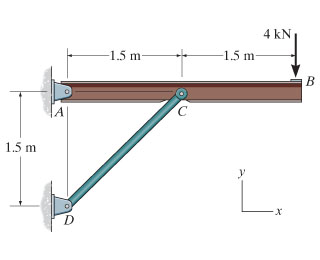
\includegraphics[width=3in]{beam.png}
\end{center}
\caption{
This is a typical example of a statics problem encountered by engineers. The goal is to understand the reactions of the pins at $A$ and $D$. \label{statics figure} Courtesy of \href{http://www.chegg.com/homework-help/questions-and-answers/draw-free-body-diagram-beam-determine-horizontal-vertical-components-beam-determine-magnit-q2963278}{chegg.com}. }
\end{figure}

To solve this type of problem, engineers apply two conservation laws.
\begin{enumerate}
 \item The first law is that the net force acting on the beam must equal the sum of individual forces acting on the beam. Since the beam is not moving (zero total net force), the sum of all forces acting on the beam is zero.  
 \item The second law is that the net torque (tendency to rotate) at every point must be zero.  Engineers use the word ``moment'' to compute torques. The process involves picking any point in the system. The moment about this point contributed by force $\vec F_i$ whose displacement from the point is $\vec d_i$ is the cross product $\vec d_i\times \vec F_i$. If we sum these torques, it must equal zero or else the rigid body will rotate.  
\end{enumerate}
Engineers spend a year practicing these ideas, and become quite fast at solving these kind of computations.  Let's walk through a computation, and then see how kernels, bases, and eigenspaces simplify the work and allow us to rapidly compute rather complex problems with ease.


\begin{problem}[Statics]
 Consider the beam diagram in Figure \ref{statics figure}. We'll first solve this exact problem for the reactions at $A$ and $D$.  Then we'll make the force $B_y$ unknown, and vary the distances. On this problem your job is to write a system of equations, and then row reduce 4 matrices. Use software. 
\begin{enumerate}
 \item The pins at $A$ and $D$ apply the forces $\vec F_A=(A_x,A_y)$ and $\vec F_D=(D_x,D_y)$ to the system consisting of the beam and rod.  The third force at $B$ is $\vec F_B=(0,B_y)=(0,-4)$ kN. Summing the forces in the $x$ direction gives the equation $A_x+D_x+0=0$. What equation do you get from summing the $y$ components? 
 \item We know $D_x=D_y$ because the rod is attached to the wall at a 45 degree angle. If instead the segment $AD$ has distance $d$ and the segment $AC$ has distance $c$, explain why $D_xd-D_yc=0$. [Think similar triangles.]  
 \item We can sum the moments about any point we choose.  The simplest point in this problem might be $C$. Summing the moments about this point gives us  $(-3/2) A_y+(3/2)B_y=0$. We now have the system of equations
$$\bvec{
1&0&1&0\\
0&1&0&1\\
0&0&1&-1\\
0&-3/2&0&0
}
\bvec{A_x\\A_y\\D_x\\D_y}
=\bvec{0\\4\\0\\(-3/2)(-4)}.$$
Solve this system to get the reactions at $A$ and $D$. 
 \item Instead of using $B_y=-4$, let's now assume that $B_y$ is an unknown force (use it as the last variable so it will become the free variable). Show how to rewrite the equation above as the homogeneous matrix equation
$$\bvec{
1&0&1&0&0\\
0&1&0&1&1\\
0&0&1&-1&0\\
0&-3/2&0&0&3/2
}
\bvec{A_x\\A_y\\D_x\\D_y\\B_y}
=\bvec{0\\0\\0\\0}.$$
Solve this system. Give a basis for kernel. If $B_y=-8$, what is $A_x$? 
 \item Continue to assume that $B_y$ is an unknown force. Let's change the distance $AD$ to be 8, the distance $AC$ to be 4, and the distance $CB$ to be 5. We can then write the system of equations as 
$$\bvec{
1&0&1&0&0\\
0&1&0&1&1\\
0&0&8&-4&0\\
0&-4&0&0&5
}
\bvec{A_x\\A_y\\D_x\\D_y\\B_y}
=\bvec{0\\0\\0\\0}.$$
Solve the system by giving a basis for the kernel. If $B_y=-8$, what is $A_x$?
 \item Continue to assume that $B_y$ is an unknown force. Let's change the distance $AD$ to be $d$, the distance $AC$ to be $4$, and the distance $CB$ to be $b$. We can then write the system of equations as 
$$\bvec{
1&0&1&0&0\\
0&1&0&1&1\\
0&0&d&-c&0\\
0&-c&0&0&b
}
\bvec{A_x\\A_y\\D_x\\D_y\\B_y}
=\bvec{0\\0\\0\\0}.$$
Solve the system by giving a basis for the kernel. 
\end{enumerate}
\end{problem}
%end 16





%17
%\mysubsection{\ideacon}
\subsubsection*{Kirchoff's Electrical Laws}
Gustav Kirchoff discovered two laws of electricity that pertain to the conservation of charge and energy.  To describe these laws, we must first discuss voltage, resistance, and current.  
\begin{itemize}
 \item Current is the flow of electricity. We'll often compare it to water flow or traffic flow.
 \item As a current passes across a conductor, it encounters resistance. Ohm's law states that the product of the resistance $R$ and current $I$ across a conductor equals the voltage $V$, i.e. $RI=V$. If the voltage remains constant, then a large resistance corresponds to a small current. 
 \item A resistor is an object with high resistance which is placed in an electrical system to slow down the flow (current) of electricity.  Resistors are measured in terms of ohms. The larger the ohms, the smaller the current.   
\end{itemize}
Figure \ref{ecir} illustrates two introductory electrical systems.
\begin{figure}
\begin{center}
\begin{tabular}{cc}
\renewcommand{\myscale}{.3}
\begin{tikzpicture}[scale=\myscale,inner sep=1pt]
%\draw[help lines,step=1cm] (0,0) grid (12,6);

%Source - like a battery
\node[label=right:$E$] at (0,3)
{{\begin{tikzpicture}[scale=\myscale]
%	\useasboundingbox (-.5,-3) rectangle (.5,3);
	\draw (0,0) circle (1cm);
	\draw (.3,.5) -- (-.3,.5);
	\draw (0,.2) -- (0,.8);
	\draw (.3,-.5) -- (-.3,-.5);
	\draw (0,1) -- (0,3);
	\draw (0,-1) -- (0,-3);
	\end{tikzpicture}
}};

%Resistor
\node[label=right:$R_2$] at (6,3) 
{{\begin{tikzpicture}[scale=\myscale]
%	\useasboundingbox (0,-3) rectangle (0,3);
	\draw (0,-3) -- ++(0,1.8) -- ++(.5,.2) 
		-- ++(-1,.4) -- ++(1,.4)
		-- ++(-1,.4) -- ++(1,.4)
		-- ++(-1,.4) -- ++(.5,.2)
		-- ++(0,1.8) ;
	\end{tikzpicture}
}};

%Resistor
\node[label=above:$R_1$] at (3,0) 
{{\begin{tikzpicture}[scale=\myscale,rotate=90]
%	\useasboundingbox (0,-3) rectangle (0,3);
	\draw (0,-3) -- ++(0,1.8) -- ++(.5,.2) 
		-- ++(-1,.4) -- ++(1,.4)
		-- ++(-1,.4) -- ++(1,.4)
		-- ++(-1,.4) -- ++(.5,.2)
		-- ++(0,1.8) ;
	\end{tikzpicture}
}};

%Resistor
\node[label=right:$R_3$] at (12,3) 
{{\begin{tikzpicture}[scale=\myscale,rotate=0]
%	\useasboundingbox (0,-3) rectangle (0,3);
	\draw (0,-3) -- ++(0,1.8) -- ++(.5,.2) 
		-- ++(-1,.4) -- ++(1,.4)
		-- ++(-1,.4) -- ++(1,.4)
		-- ++(-1,.4) -- ++(.5,.2)
		-- ++(0,1.8) ;
	\end{tikzpicture}
}};

%Straight Path
\node at (3,6) 
{{\begin{tikzpicture}[scale=\myscale,rotate=90]
	\draw (0,-3) -- (0,3);
	\end{tikzpicture}
}};

%Straight Path
\node at (9,6) 
{{\begin{tikzpicture}[scale=\myscale,rotate=90]
	\draw (0,-3) -- (0,3);
	\end{tikzpicture}
}};

%Straight Path
\node at (9,0) 
{{\begin{tikzpicture}[scale=\myscale,rotate=90]
	\draw (0,-3) -- (0,3);
	\end{tikzpicture}
}};


%Arrow to represent Current
\node[label=above:$i_1$] at (3,6) 
{{\begin{tikzpicture}[scale=\myscale,rotate=-90]
%	\useasboundingbox (0,-.4) rectangle (0,.4);
	\filldraw (0,.4) -- (-.2,-.4) -- (0,-.3) -- (.2,-.4);
	\end{tikzpicture}
}};

%Arrow to represent Current
\node[label=right:$i_2$] at (6,5) 
{{\begin{tikzpicture}[scale=\myscale,rotate=180]
%	\useasboundingbox (0,-.4) rectangle (0,.4);
	\filldraw (0,.4) -- (-.2,-.4) -- (0,-.3) -- (.2,-.4);
	\end{tikzpicture}
}};

%Arrow to represent Current
\node[label=above:$i_3$] at (9,6) 
{{\begin{tikzpicture}[scale=\myscale,rotate=-90]
%	\useasboundingbox (0,-.4) rectangle (0,.4);
	\filldraw (0,.4) -- (-.2,-.4) -- (0,-.3) -- (.2,-.4);
	\end{tikzpicture}
}};

%Node
\node at (6,6) 
{{\begin{tikzpicture}[scale=\myscale,rotate=-90]
%	\useasboundingbox (0,-.4) rectangle (0,.4);
	\filldraw (0,0) circle (.15cm);
	\end{tikzpicture}
}};

%Node
\node at (6,0) 
{{\begin{tikzpicture}[scale=\myscale,rotate=-90]
%	\useasboundingbox (0,-.4) rectangle (0,.4);
	\filldraw (0,0) circle (.15cm);
	\end{tikzpicture}
}};

\end{tikzpicture}

&
\renewcommand{\myscale}{.3}
\begin{tikzpicture}[scale=\myscale,inner sep=1pt]
%\draw[help lines,step=1cm] (0,0) grid (18,6);

%Source - like a battery
\node[label=right:$E$] at (0,3) 
{{\begin{tikzpicture}[scale=\myscale]
%	\useasboundingbox (-.5,-3) rectangle (.5,3);
	\draw (0,0) circle (1cm);
	\draw (.3,.5) -- (-.3,.5);
	\draw (0,.2) -- (0,.8);
	\draw (.3,-.5) -- (-.3,-.5);
	\draw (0,1) -- (0,3);
	\draw (0,-1) -- (0,-3);
	\end{tikzpicture}
}};

%Resistor
\node[label=right:$R_2$] at (6,3) 
{{\begin{tikzpicture}[scale=\myscale]
%	\useasboundingbox (0,-3) rectangle (0,3);
	\draw (0,-3) -- ++(0,1.8) -- ++(.5,.2) 
		-- ++(-1,.4) -- ++(1,.4)
		-- ++(-1,.4) -- ++(1,.4)
		-- ++(-1,.4) -- ++(.5,.2)
		-- ++(0,1.8) ;
	\end{tikzpicture}
}};

%Resistor
\node[label=above:$R_1$] at (3,0) 
{{\begin{tikzpicture}[scale=\myscale,rotate=90]
%	\useasboundingbox (0,-3) rectangle (0,3);
	\draw (0,-3) -- ++(0,1.8) -- ++(.5,.2) 
		-- ++(-1,.4) -- ++(1,.4)
		-- ++(-1,.4) -- ++(1,.4)
		-- ++(-1,.4) -- ++(.5,.2)
		-- ++(0,1.8) ;
	\end{tikzpicture}
}};

%Resistor
\node[label=above:$R_3$] at (9,6) 
{{\begin{tikzpicture}[scale=\myscale,rotate=90]
%	\useasboundingbox (0,-3) rectangle (0,3);
	\draw (0,-3) -- ++(0,1.8) -- ++(.5,.2) 
		-- ++(-1,.4) -- ++(1,.4)
		-- ++(-1,.4) -- ++(1,.4)
		-- ++(-1,.4) -- ++(.5,.2)
		-- ++(0,1.8) ;
	\end{tikzpicture}
}};

%Resistor
\node[label=right:$R_4$] at (12,3) 
{{\begin{tikzpicture}[scale=\myscale,rotate=0]
%	\useasboundingbox (0,-3) rectangle (0,3);
	\draw (0,-3) -- ++(0,1.8) -- ++(.5,.2) 
		-- ++(-1,.4) -- ++(1,.4)
		-- ++(-1,.4) -- ++(1,.4)
		-- ++(-1,.4) -- ++(.5,.2)
		-- ++(0,1.8) ;
	\end{tikzpicture}
}};

%Resistor
\node[label=right:$R_5$] at (18,3) 
{{\begin{tikzpicture}[scale=\myscale,rotate=0]
%	\useasboundingbox (0,-3) rectangle (0,3);
	\draw (0,-3) -- ++(0,1.8) -- ++(.5,.2) 
		-- ++(-1,.4) -- ++(1,.4)
		-- ++(-1,.4) -- ++(1,.4)
		-- ++(-1,.4) -- ++(.5,.2)
		-- ++(0,1.8) ;
	\end{tikzpicture}
}};

%Resistor
\node[label=above:$R_6$] at (9,0) 
{{\begin{tikzpicture}[scale=\myscale,rotate=90]
%	\useasboundingbox (0,-3) rectangle (0,3);
	\draw (0,-3) -- ++(0,1.8) -- ++(.5,.2) 
		-- ++(-1,.4) -- ++(1,.4)
		-- ++(-1,.4) -- ++(1,.4)
		-- ++(-1,.4) -- ++(.5,.2)
		-- ++(0,1.8) ;
	\end{tikzpicture}
}};









%Straight Path
\node at (3,6) 
{{\begin{tikzpicture}[scale=\myscale,rotate=90]
	\draw (0,-3) -- (0,3);
	\end{tikzpicture}
}};

%Straight Path
\node at (15,6) 
{{\begin{tikzpicture}[scale=\myscale,rotate=90]
	\draw (0,-3) -- (0,3);
	\end{tikzpicture}
}};

%Straight Path
\node at (15,0) 
{{\begin{tikzpicture}[scale=\myscale,rotate=90]
	\draw (0,-3) -- (0,3);
	\end{tikzpicture}
}};






%Arrow to represent Current
\node[label=above:$i_1$] at (3,6) 
{{\begin{tikzpicture}[scale=\myscale,rotate=-90]
%	\useasboundingbox (0,-.4) rectangle (0,.4);
	\filldraw (0,.4) -- (-.2,-.4) -- (0,-.3) -- (.2,-.4);
	\end{tikzpicture}
}};

%Arrow to represent Current
\node[label=right:$i_2$] at (6,5) 
{{\begin{tikzpicture}[scale=\myscale,rotate=180]
%	\useasboundingbox (0,-.4) rectangle (0,.4);
	\filldraw (0,.4) -- (-.2,-.4) -- (0,-.3) -- (.2,-.4);
	\end{tikzpicture}
}};

%Arrow to represent Current
\node[label=above:$i_3$] at (7,6) 
{{\begin{tikzpicture}[scale=\myscale,rotate=-90]
%	\useasboundingbox (0,-.4) rectangle (0,.4);
	\filldraw (0,.4) -- (-.2,-.4) -- (0,-.3) -- (.2,-.4);
	\end{tikzpicture}
}};

%Arrow to represent Current
\node[label=right:$i_4$] at (12,5) 
{{\begin{tikzpicture}[scale=\myscale,rotate=180]
%	\useasboundingbox (0,-.4) rectangle (0,.4);
	\filldraw (0,.4) -- (-.2,-.4) -- (0,-.3) -- (.2,-.4);
	\end{tikzpicture}
}};

%Arrow to represent Current
\node[label=above:$i_5$] at (15,6) 
{{\begin{tikzpicture}[scale=\myscale,rotate=-90]
%	\useasboundingbox (0,-.4) rectangle (0,.4);
	\filldraw (0,.4) -- (-.2,-.4) -- (0,-.3) -- (.2,-.4);
	\end{tikzpicture}
}};

%Arrow to represent Current
\node[label=above:$i_6$] at (11,0) 
{{\begin{tikzpicture}[scale=\myscale,rotate=90]
%	\useasboundingbox (0,-.4) rectangle (0,.4);
	\filldraw (0,.4) -- (-.2,-.4) -- (0,-.3) -- (.2,-.4);
	\end{tikzpicture}
}};








%Node
\node at (6,6) 
{{\begin{tikzpicture}[scale=\myscale,rotate=-90]
%	\useasboundingbox (0,-.4) rectangle (0,.4);
	\filldraw (0,0) circle (.15cm);
	\end{tikzpicture}
}};

%Node
\node at (6,0) 
{{\begin{tikzpicture}[scale=\myscale,rotate=-90]
%	\useasboundingbox (0,-.4) rectangle (0,.4);
	\filldraw (0,0) circle (.15cm);
	\end{tikzpicture}
}};

%Node
\node at (12,0) 
{{\begin{tikzpicture}[scale=\myscale,rotate=-90]
%	\useasboundingbox (0,-.4) rectangle (0,.4);
	\filldraw (0,0) circle (.15cm);
	\end{tikzpicture}
}};

%Node
\node at (12,6) 
{{\begin{tikzpicture}[scale=\myscale,rotate=-90]
%	\useasboundingbox (0,-.4) rectangle (0,.4);
	\filldraw (0,0) circle (.15cm);
	\end{tikzpicture}
}};

\end{tikzpicture}

\\
Two Loop System & Three Loop System
\end{tabular}\end{center}
\caption{Electrical Circuit Diagrams.\label{ecir}}
\end{figure}
In this diagram, wires meet at nodes (illustrated with a dot).  
Batteries and voltage sources (represented by 
\begin{tikzpicture}[scale=.15,rotate=-90]
%	\useasboundingbox (-.5,-3) rectangle (.5,3);
	\clip (-1,-2) rectangle (1,2);
	\draw (0,0) circle (1cm);
	\draw (.3,.5) -- (-.3,.5);
	\draw (0,.2) -- (0,.8);
	\draw (.3,-.5) -- (-.3,-.5);
	\draw (0,1) -- (0,3);
	\draw (0,-1) -- (0,-3);
\end{tikzpicture}
or other symbols)
supply a voltage of $E$ volts.  At each node the current may change, so the arrows and letters $i$ represent the different currents in the electrical system. The electrical current on each wire may or may not follow the arrows drawn (a negative current means that the current flows opposite the arrow). Resistors are depicted with the symbol 	
\begin{tikzpicture}[scale=.2,rotate=90]
%	\useasboundingbox (0,-3) rectangle (0,3);
	\clip (-.5,-2) rectangle (.5,2);
	\draw (0,-3) -- ++(0,1.8) -- ++(.5,.2) 
		-- ++(-1,.4) -- ++(1,.4)
		-- ++(-1,.4) -- ++(1,.4)
		-- ++(-1,.4) -- ++(.5,.2)
		-- ++(0,1.8) ;
	\end{tikzpicture}
, and the letter $R$ represents the ohms. 

Kirchoff discovered two laws. They both help us find current in a system, provided we know the voltage of any batteries, and the resistance of any resistors. 
\begin{enumerate}
	\item Kirchoff's current law states that at every node, the current flowing in equals the current flowing out (at nodes, current in = current out). 
	\item Kirchoff's voltage law states that on any loop in the system, the directed sum of voltages supplied equals the directed sum of voltage drops (in loops, voltage in = voltage out). To use this law, pick a spot in the system.  Then move around the system following a path that eventually gets you back to where you began (a closed curve). If you encounter a battery (a voltage source), then it counts as voltage in.  If you encounter a resistor as you move with the current, then the voltage drop is $Ri$.  If you encounter a resistor while moving opposite the current, then times by a negative to get a voltage drop of $-R_i$.
\end{enumerate}

Let's use Kirchoff's laws to generate a system of equations for the two loop system. Remember that every time a current encounters a resistor, the voltage drop is $V=RI$, the product of the resistance and the current. 
\begin{problem} \label{kirchoff 2 loop general}
Consider the two loop system in figure \ref{ecir}. Assume that the voltage supplied from the battery $E$, as well as the ohms $R_1$, $R_2$, and $R_3$, on the resistors are known. The currents $i_1$, $i_2$, and $i_3$ are unknown.
\begin{enumerate}
 \item Use Kirchoff's laws to explain how to obtain each of the equations below:
$$
\begin{array}{rl}
i_1-i_2-i_3&=0\\
-i_1+i_2+i_3&=0\\
R_1i_1+R_2i_2-E&=0\\
-R_2 i_2 +R_3i_3&=0.\\
R_1i_1 + R_3i_3-E&=0.
\end{array}
%\quad \Rightarrow
%\bvec{
%1&-1&-1&0\\
%-1&1&1&0\\
%R_1&R_2&0&-1\\
%0&-R_2&R_3&0\\
%R_1&0&R_3&-1
%}
%\bvec{i_1\\i_2\\i_3\\E}
%=\bvec{0\\0\\0\\0\\0}
$$
[Hint: If you encounter a resistor while moving backwards along a loop, then the voltage drop becomes a voltage gain (times by a negative).]
 \item Some of the equations above are linear combinations of the other equations.  How could you obtain the 2nd and 5th as a linear combination of the others?
 \item Suppose $R_1 = 2$, $R_2 = 3$, and  $R_3 = 6$ ohms.  Solve the system of equations above by row reducing an appropriate matrix (think of $E$ as an unknown and find the kernel of a matrix).  State a basis for the solutions.
 \item If we know the power source is $E=12$ V, what is $i_1$?  If we measure the current in the first wire to be $i_1=10$ amps, then what is $E$?
\end{enumerate}
\end{problem}
%end 17













%18
\mysubsection{\ideapro}
When we want to find the coefficients of an equation such as $y=mx+b$ or $y=ax^2+bx+c$ that passes through several points, remember that the key idea is to write the linear system of equations $A\vec x=\vec b$ that we wish to solve.  If the equation has no solution, then we multiply both sides by $A^T$ and then solve the corresponding system.  This gets us the linear combination of the columns of $A$ that is closest to $\vec b$. We call this linear regression. 
%Change this to just 5 points through a parabola.
\begin{problem}
 Consider the 5 points 
$$ 
(-1,  1),
( 0, -1),
( 1, -2),
( 2, -1),
( 2, -2)
$$
\begin{enumerate}
 \item Use linear regression to give an equation of the line $y=a_0+a_1x$ that best fits these 5 points. (Remember to set up the system $A\vec x = \vec b$, and then multiply on the left by the transpose $A^T$.) 
 \item Use linear regression to give an equation of the parabola $y=a_0+a_1x+a_2x^2$ that best fits these 5 points. 
 For this one, your system $A\vec x=\vec b$ looks like 
 $$\bvec{\nvec{1\\1\\1\\1\\1}&\nvec{-1\\0\\1\\2\\2}&\nvec{?\\?\\?\\?\\?}}\bvec{a_0\\a_1\\a_2}=\bvec{1\\-1\\-2\\-1\\-2}.$$ Just multiply both sides by $A^T$ and then solve the system of equations. The coefficients are rather ugly (one is $-115/78$).
 \item Use linear regression to give an equation of the cubic $y=a_0+a_1x+a_2x^2+a_3x^3$ that best fits these 5 points. Your answer should have some $1/12$ths in it. Graph your solution. 
 \item Why is there no quartic that passes exactly through these points?
\end{enumerate}
When you finish this problem, you should have three setups of the form $A\vec x=\vec b$. You should also show what equation you get after multiplying by $A^T$ on both sides.  Then show the rref of the resulting system, and write the equation of the line, parabola, and cubic that you obtain. 
\end{problem}
%end 18









%19
When the number of points matches the number of unknown coefficients, we can find an equation of the model without using linear regression. To organize our work, let's first standardize the notation.  Rather than writing $y=mx+b$, let's write $y=a_0+a_1 x$ (where $a_0=b$ and $a_1=m$). For a parabola, let's write $\ds y=a_0 + a_1 x+ a_2 x^2 = \sum_{k=0}^{2} a_k x^k$. We can now write any polynomial in the form $$\ds y = a_0 + a_1 x+ \cdots + a_n x^n = \sum_{k=0}^n a_k x^k.$$ By standardizing the coefficients, we can use summation notation to express any degree polynomial by changing the $n$ on the top of the summation sign. 

%\mysubsection{\ideapro}
%Way too long.  Just shave off a few parts, and this would be perfect.  The engineers didn't struggle with this problem any.  It might be a better problem at the opening.
\begin{problem}
 Answer the following by row reducing an appropriate matrix (just use software). [Hint: Each point produces an equation.]
\begin{enumerate}
 \item 
Find the intercept $a_0$ and slope $a_1$ of a line $y = a_0+a_1 x$ that passes through the points $(1,2)$ and $(3,5)$. [We could have used $m$ and $b$, but I chose to use $a_0$ and $a_1$ so we can see how this generalizes to all dimensions.]
 \item 
Find the coefficients $a_0$, $a_1$, and $a_2$ of a parabola $y = a_0+a_1 x^1+a_2x^2$ that passes through the points $(0, 1)$,  $(2, 3)$, and  $(−1, 4)$. [Hint: The second point produces the equation $3=a_0+a_1(2)+a_2(2)^2$.]
 \item
Give an equation of a cubic polynomial $y = a_0+a_1x^1+a_2x^2+a_3x^3$ that passes through the four points $(0, 1)$, $(1, 3)$, $(−1, 4)$, and $(2, 4)$. [You should have a linear system with 4 equations and 4 unknowns.]
\item 
Suppose that we collect the 6 data points $(1,1)$, $(2,3)$, $(-1,2)$, $(0,-1)$, $(-2,0)$, $(3,1)$, and we would like to find a polynomial that passes through all 6 points. State the degree $n$ of this polynomial. Then find the coefficients $a_0, a_1, \ldots, a_n$ of this polynomial. Use technology to do your row reduction.  When you present in class, show us the matrix you entered into a computer, and then show us the reduced row echelon form together with the polynomial.
\end{enumerate}
\end{problem}
%end 19













\mysubsection{\idealin}


%20
\subsubsection*{Cramer's Rule}
Gabriel Cramer developed a way to solve linear systems of equations by using determinants. For small systems, the solution is extremely fast.  For large systems the method looses its power because of the complexity of computing determinants.  However, when the coefficients in the system are variables, Cramer's rule provides an extremely fast algorithm for obtaining solutions. I'll remind you occasionally throughout the problem set to apply Cramer's rule when the problem involves variable coefficients.
\begin{problem}[Cramer's Rule]
Our goal on this problem is to find a quick way to solve the matrix equation $$\begin{bmatrix}\nvec{a_{11}\\a_{21}}&\nvec{a_{12}\\a_{22}} \end{bmatrix}
\begin{bmatrix}\nvec{x_{1}\\x_{2}} \end{bmatrix}
=
\begin{bmatrix}\nvec{b_{1}\\b_{2}} \end{bmatrix}.$$ 
Let's look at an example and from it develop a general rule. 
Let $\vec v_1 = (a_{11},a_{21})=(2,-2)$ and $\vec v_2 = (a_{12},a_{22})= (1,2)$, so $A=\bvec{2&1\\-2&2}$. If we know that $x_1=-3$ and $x_2 = -2$, the we have $\vec b = x_1\vec v_1+x_2\vec v_2=(-8,2)$. In the picture below, the solid red vector is $\vec v_1$, the solid blue vector is $\vec v_2$, and the solid black vector is $\vec b$. Use the picture below, to answer the questions that follow.

%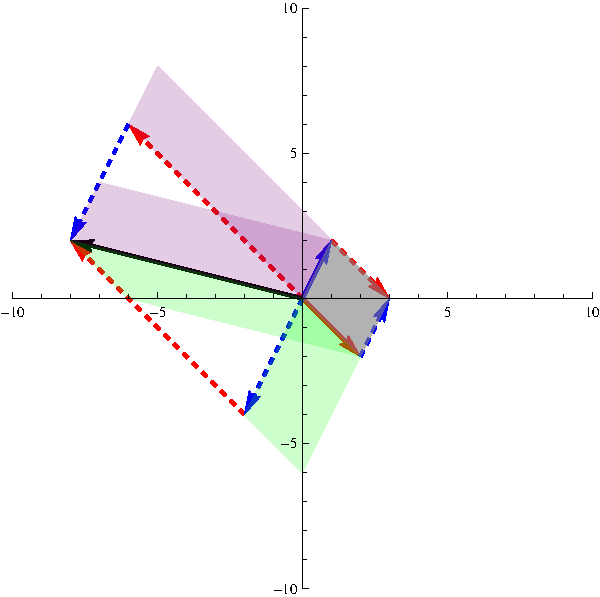
\includegraphics{cramers-visual}

\begin{center}
 \begin{tikzpicture}[scale=.5]
  \fill[lightgray] (0,0) -- (2,-2) -- (3,0) -- (1,2) -- (0,0);
  \fill[color=red!50!blue,opacity=0.2] (0,0) -- ++(1,2) -- ++(-6,6) -- ++(-1,-2) -- ++(6,-6);
  \fill[color=red!50!blue,opacity=0.2] (0,0) -- ++(1,2) -- ++(-8,2) -- ++(-1,-2) -- ++(8,-2);
  \fill[color=green,opacity=0.2] (0,0) -- ++(2,-2) -- ++(-8,2) -- ++(-2,2) -- ++(8,-2);
  \fill[color=green,opacity=0.2] (0,0) -- ++(2,-2) -- ++(-2,-4) -- ++(-2,2) -- ++(2,4);
  %axis
  \draw (-8,0) -- coordinate (x axis mid) (4,0);
  \draw (0,-6) -- coordinate (y axis mid) (0,8);
  %ticks
  \foreach \x in {-8,...,4}
   \draw (\x,1pt) -- (\x,-3pt)
    node[anchor=north] {};
  \foreach \y in {-6,...,8}
   \draw (1pt,\y) -- (-3pt,\y) 
    node[anchor=east] {}; 
  \draw[red,->,very thick] (0,0) -- (2,-2);
  \draw[blue,->,very thick] (0,0) -- (1,2);
  \draw[black,->,very thick] (0,0) -- (-8,2);
  \draw[red,->,very thick,dashed] (1,2) -- ++(2,-2);
  \draw[blue,->,very thick,dashed] (2,-2) -- ++(1,2);
  \draw[red,->,very thick,dashed] (0,0) -- ++(-6,6);
  \draw[red,->,very thick,dashed] (-2,-4) -- ++(-6,6);
  \draw[blue,->,very thick,dashed] (0,0) -- ++(-2,-4);
  \draw[blue,->,very thick,dashed] (-6,6) -- ++(-2,-4);
 \end{tikzpicture}
\end{center}


\noindent[Hint: Each question can be answered by thinking about determinants as areas.]
\begin{enumerate}
 \item 
 \marginpar{Remember that when we put vertical bars on a matrix, that means we compute the determinant.}%
 Explain why $x_1\begin{vmatrix}\vec{v_1}&\vec v_2\end{vmatrix}=\begin{vmatrix}x_1\vec{v_1}&\vec v_2\end{vmatrix}$.  
\item Now explain why $\begin{vmatrix}x_1\vec{v_1}&\vec v_2\end{vmatrix} = \begin{vmatrix}\vec{b}&\vec v_2\end{vmatrix}$. [Hint: Why do the two purple parallelograms have the same area?]  
 \item Finally, solve for $x_1$ to show that $$x_1 = \frac{\begin{vmatrix}\nvec{b_1\\b_2}&\nvec{a_{12}\\a_{22}} \end{vmatrix}}{\begin{vmatrix}\nvec{a_{11}\\a_{21}}&\nvec{a_{12}\\a_{22}} \end{vmatrix}}.$$
 \item In a similar fashion, show that $$x_2 =\frac{\begin{vmatrix}\nvec{a_{11}\\a_{21}}&\nvec{b_1\\b_2}\end{vmatrix}}{\begin{vmatrix}\nvec{a_{11}\\a_{21}}&\nvec{a_{12}\\a_{22}} \end{vmatrix}}.$$ 
 \item Consider the system of equations $x+2y=3, 4x+5y=6$. Use the formulas you just developed to solve this system. You'll need to compute three determinants.
 \end{enumerate}
\end{problem}




The previous problem is a proof by picture of Cramer's rule in 2D. The proof of the theorem is similar in all dimensions. The key idea is to connect determinants to area.  
Here's a formal statement of Cramer's Rule.
\begin{theorem}[Cramer's Rule]\label{Cramer's Rule}
 Consider the linear system given by $A\vec x = \vec b$, where 
$A=\begin{bmatrix}\vec v_1 &\vec v_2 &\cdots \vec v_n \end{bmatrix}$
is an $n$ by $n$ matrix whose determinant is not zero.  Let $D=|A|$. For each $i$, replace vector $\vec v_i$ with $\vec b$, and then let $D_i$ be the determinant of the corresponding matrix. The solution to the linear system is
$$x_1 = \frac{D_1}{D},\quad x_2 = \frac{D_2}{D},\quad \cdots \quad x_n = \frac{D_n}{D}.$$

For the 2 by 2 system
$$
\begin{bmatrix}\nvec{a_{11}\\a_{21}}&\nvec{a_{12}\\a_{22}} \end{bmatrix}
\begin{bmatrix}\nvec{x_{1}\\x_{2}} \end{bmatrix}
=
\begin{bmatrix}\nvec{b_{1}\\b_{2}} \end{bmatrix},
$$
Cramer's rule states the solution is (provided $|A|\neq 0$) 
$$
x_1 = \frac{D_1}{D}=\frac{\begin{vmatrix}\nvec{b_1\\b_2}&\nvec{a_{12}\\a_{22}} \end{vmatrix}}{\begin{vmatrix}\nvec{a_{11}\\a_{21}}&\nvec{a_{12}\\a_{22}} \end{vmatrix}},
\quad 
x_2 = \frac{D_2}{D}=\frac{\begin{vmatrix}\nvec{a_{11}\\a_{21}}&\nvec{b_1\\b_2}\end{vmatrix}}{\begin{vmatrix}\nvec{a_{11}\\a_{21}}&\nvec{a_{12}\\a_{22}} \end{vmatrix}}
.$$
\end{theorem}
%end 20











%21
\mysubsection{\ideapro}
\begin{problem}
Solve the following. [Hint: Because the problem involves variable points, Cramer's rule will be much faster than row reduction.]
\begin{enumerate}
 \item Find the intercept $a_0$ and slope $a_1$ of a line $y = a_0+a_1 x$ that passes through the points $(x_1,y_1)$ and $(x_2,y_2)$. 
 \item Use Cramer's rule to state the coefficients $a_1$ of a parabola $y = a_0+a_1 x^1+a_2x^2$ that passes through the points $(x_1, y_1)$,  $(x_2, y_2)$, and  $(x_3, y_3)$. You could similarly find $a_0$ and $a_2$, but don't worry about it.
\end{enumerate}
Can you think of any conditions where your solutions above will not be valid?
\end{problem}
%end 21













%22
%\mysubsection{\ideapro}

We've seen how to linear regression to find an equation of lines, parabolas, cubics, and more that best fit several data points. The key is to set up a system which has no solution, multiply both sides on the left by the transpose, and then solve. Let's use this idea to obtain a general solution for finding an equation of the linear regression line that best approximates some arbitrary points. 

%Do 5 points through a line.  Leave them general.
\begin{problem}
 Consider the five points 
 $$
 (x_1,y_1),
 (x_2,y_2),
 (x_3,y_3),
 (x_4,y_4),
 (x_5,y_5).
$$
We would like to find an equation of the least squares regression line $y=a_0+a_1x$ that best fits these points. 
Set up the matrices $A$, $\vec x$, $\vec b$, and $A^T$. Multiply together $A^TA$ and $A^T\vec b$ (your result should involve sums of the form $\sum x_i$, $\sum y_i$, $\sum x_iy_i$, and $\sum x_i^2$). Then solve the equation $A^TA\vec x = A^T\vec b$ and state the coefficients $a_0$ and $a_1$. 

[Hint: Since the system involves variable coefficients, try using Cramer's rule. It should kick out the solution almost instantly with 3 two by two determinants. One of these determinants should be $(5)\left(\sum x_iy_i\right) - \left(\sum x_i\right)\left(\sum y_i\right)$.]
\end{problem}

The formula you developed above is the formula found in software programs.  It's also the formula you'll find in statistic textbooks, high school textbooks, online help sites, etc.  They just change the $5$ to an $n$. 
% This concept is one that you can help students in high school understand.  Most books just say, ``Multiply by $A^T$,'' but never give a reason why you would do that.  You can help students understand that $A\vec x$ is a linear combination of the columns of $A$, and that regression just asks them to find the linear combination that gets them closest to $\vec b$. 
%end 22





%\end{document}






%23
\mysubsection{\ideanon}
\subsubsection*{The Arms Race}
%Cramer's rule is most useful when the coefficients in the linear system are variables, rather than numbers.  
Let's apply our knowledge to study the arms race (the building of armies - tanks, bombs, soldiers, etc. - between two countries).  Consider two countries, country $A$ and country $B$. As country $B$ builds up their military, country $A$ looks on and says ``Hmm, we better build up our military.''  Similarly, as country $A$ builds up their military, country $B$ says the same. If country $A$ has a grudge against country $B$, they will probably build up their military regardless of what country $B$ does.  Similarly, any past grievances and grudges that country $B$ has against country $A$ will increase the rate at which country $B$ builds up their military. Building up a military costs money, so hopefully both countries have economic limitations that restrict the growth of their military. The real question behind the arms race is,
\begin{quote}
 Will the two countries eventually decide they are spending enough on their military, or will their spending continue to grow without bound.
\end{quote}

 We now develop a system of differential equations that describes the above. We've seen the idea ``flow in equals flow out'' in our conservation problems.  In this case, arms are not conserved.  Instead, we have the following rule:
\begin{quote}
 The change in a quantity equals the flow in of the quantity minus the flow out of the quantity, or more simply 
$$\text{Change = (Flow in) - (Flow out)}$$
$$\text{Change = (Increase) - (Decrease)}$$
\end{quote}
\begin{itemize}
\item Let $x$ represent the dollar amount per year that country $A$ spends on arms. Let $y$ represent the dollar amount per year that country $B$ spends on arms.  
\item When $y$ is large, country $A$ will respond by increasing their spending.  
We'll assume this change is proportional to $y$, so we see that $x$ increases by an amount $ay$. 
 Similarly, when $x$ is large, country $B$ responds by increasing their spending. Let's assume that $y$ increases by an amount $mx$.
\item The economy of each country tries to slow down the spending rate.  The more money country $A$ spends, the larger the effect of the economy.  We'll assume that $x$ decreases by an amount proportional to itself, namely $bx$.  Similarly, we'll assume $y$ decrease by an amount $ny$.
\item If the countries hold grudges against each other for past grievances, then they are inclined to increase their spending regardless of economic factors and the growth of the other country's army.  Let $c$ represent the amount that country $A$ will increase their spending by, and let $p$ represent the amount that country $B$ will increase their spending by. These values might be zero (for example the US and Canada do not hold such grudges), but might not be zero at all (as was the case during the cold war, between the US and USSR).
\end{itemize}

\begin{problem}
Start by reading the arms race information above.
\begin{enumerate}
 \item There are three things causing $x$ to change. The flow in (parts causing an increase) are $ay$, the response to the other country, and $c$, any grudges.  The flow out (parts causing a decrease) is only $bx$, the economic restriction.  We can write this as a differential equation $$\frac{dx}{dt} = ay+c-bx.$$ Obtain a similar equation for $\dfrac{dy}{dt}$ (using the coefficients $m$, $n$, and $p$). Then write your system of ODEs in the form 
$$
\begin{bmatrix}x'\\y'\end{bmatrix}
=
\begin{bmatrix}-b&a\\?&?\end{bmatrix}
\begin{bmatrix}x\\y\end{bmatrix}
+
\begin{bmatrix}c\\?\end{bmatrix}.
$$ 
 \item An equilibrium solution to the system of differential equations above is a solution that remains stable (flow in equals flow out). At equilibrium, there should not be any future change in $x$ nor $y$, so we should have $dx/dt=0$ and $dy/dt=0$. Find the equilibrium solution for the arms race problem. [Cramer's rule should make this really fast.]
 \item We can write the differential equation in vector field form as $(x',y') = (ay+c-bx,...)$.  Compute the derivative of this vector field to obtain a 2 by 2 matrix.  
 \item Find the eigenvalues of this matrix. [Use the quadratic formula.] 
 \item (Challenge) If any eigenvalue of this matrix is positive, then uncontrolled spending will occur. What conditions must be met so that both eigenvalues are not positive?
%In class, we'll pick some positive values for $a,b,c,m,n,p$ that satisfy the conditions you tell us, and then graph the vector field $\frac{d \vec x}{dt} = A\vec x+\vec p$, along with some solution curves.  
\end{enumerate}
\end{problem}
%end 23









\mysubsection{\ideacon}
Let's return to another problem involving Kirchoff's electrical laws. 

%24
%Change this.  Make sure it puts $E$ as a column in the matrix. 
\begin{problem}
Consider the three loop system below. 
\begin{center}
\renewcommand{\myscale}{.3}
\begin{tikzpicture}[scale=\myscale,inner sep=1pt]
%\draw[help lines,step=1cm] (0,0) grid (18,6);

%Source - like a battery
\node[label=right:$E$] at (0,3) 
{{\begin{tikzpicture}[scale=\myscale]
%	\useasboundingbox (-.5,-3) rectangle (.5,3);
	\draw (0,0) circle (1cm);
	\draw (.3,.5) -- (-.3,.5);
	\draw (0,.2) -- (0,.8);
	\draw (.3,-.5) -- (-.3,-.5);
	\draw (0,1) -- (0,3);
	\draw (0,-1) -- (0,-3);
	\end{tikzpicture}
}};

%Resistor
\node[label=right:$R_2$] at (6,3) 
{{\begin{tikzpicture}[scale=\myscale]
%	\useasboundingbox (0,-3) rectangle (0,3);
	\draw (0,-3) -- ++(0,1.8) -- ++(.5,.2) 
		-- ++(-1,.4) -- ++(1,.4)
		-- ++(-1,.4) -- ++(1,.4)
		-- ++(-1,.4) -- ++(.5,.2)
		-- ++(0,1.8) ;
	\end{tikzpicture}
}};

%Resistor
\node[label=above:$R_1$] at (3,0) 
{{\begin{tikzpicture}[scale=\myscale,rotate=90]
%	\useasboundingbox (0,-3) rectangle (0,3);
	\draw (0,-3) -- ++(0,1.8) -- ++(.5,.2) 
		-- ++(-1,.4) -- ++(1,.4)
		-- ++(-1,.4) -- ++(1,.4)
		-- ++(-1,.4) -- ++(.5,.2)
		-- ++(0,1.8) ;
	\end{tikzpicture}
}};

%Resistor
\node[label=above:$R_3$] at (9,6) 
{{\begin{tikzpicture}[scale=\myscale,rotate=90]
%	\useasboundingbox (0,-3) rectangle (0,3);
	\draw (0,-3) -- ++(0,1.8) -- ++(.5,.2) 
		-- ++(-1,.4) -- ++(1,.4)
		-- ++(-1,.4) -- ++(1,.4)
		-- ++(-1,.4) -- ++(.5,.2)
		-- ++(0,1.8) ;
	\end{tikzpicture}
}};

%Resistor
\node[label=right:$R_4$] at (12,3) 
{{\begin{tikzpicture}[scale=\myscale,rotate=0]
%	\useasboundingbox (0,-3) rectangle (0,3);
	\draw (0,-3) -- ++(0,1.8) -- ++(.5,.2) 
		-- ++(-1,.4) -- ++(1,.4)
		-- ++(-1,.4) -- ++(1,.4)
		-- ++(-1,.4) -- ++(.5,.2)
		-- ++(0,1.8) ;
	\end{tikzpicture}
}};

%Resistor
\node[label=right:$R_5$] at (18,3) 
{{\begin{tikzpicture}[scale=\myscale,rotate=0]
%	\useasboundingbox (0,-3) rectangle (0,3);
	\draw (0,-3) -- ++(0,1.8) -- ++(.5,.2) 
		-- ++(-1,.4) -- ++(1,.4)
		-- ++(-1,.4) -- ++(1,.4)
		-- ++(-1,.4) -- ++(.5,.2)
		-- ++(0,1.8) ;
	\end{tikzpicture}
}};

%Resistor
\node[label=above:$R_6$] at (9,0) 
{{\begin{tikzpicture}[scale=\myscale,rotate=90]
%	\useasboundingbox (0,-3) rectangle (0,3);
	\draw (0,-3) -- ++(0,1.8) -- ++(.5,.2) 
		-- ++(-1,.4) -- ++(1,.4)
		-- ++(-1,.4) -- ++(1,.4)
		-- ++(-1,.4) -- ++(.5,.2)
		-- ++(0,1.8) ;
	\end{tikzpicture}
}};









%Straight Path
\node at (3,6) 
{{\begin{tikzpicture}[scale=\myscale,rotate=90]
	\draw (0,-3) -- (0,3);
	\end{tikzpicture}
}};

%Straight Path
\node at (15,6) 
{{\begin{tikzpicture}[scale=\myscale,rotate=90]
	\draw (0,-3) -- (0,3);
	\end{tikzpicture}
}};

%Straight Path
\node at (15,0) 
{{\begin{tikzpicture}[scale=\myscale,rotate=90]
	\draw (0,-3) -- (0,3);
	\end{tikzpicture}
}};






%Arrow to represent Current
\node[label=above:$i_1$] at (3,6) 
{{\begin{tikzpicture}[scale=\myscale,rotate=-90]
%	\useasboundingbox (0,-.4) rectangle (0,.4);
	\filldraw (0,.4) -- (-.2,-.4) -- (0,-.3) -- (.2,-.4);
	\end{tikzpicture}
}};

%Arrow to represent Current
\node[label=right:$i_2$] at (6,5) 
{{\begin{tikzpicture}[scale=\myscale,rotate=180]
%	\useasboundingbox (0,-.4) rectangle (0,.4);
	\filldraw (0,.4) -- (-.2,-.4) -- (0,-.3) -- (.2,-.4);
	\end{tikzpicture}
}};

%Arrow to represent Current
\node[label=above:$i_3$] at (7,6) 
{{\begin{tikzpicture}[scale=\myscale,rotate=-90]
%	\useasboundingbox (0,-.4) rectangle (0,.4);
	\filldraw (0,.4) -- (-.2,-.4) -- (0,-.3) -- (.2,-.4);
	\end{tikzpicture}
}};

%Arrow to represent Current
\node[label=right:$i_4$] at (12,5) 
{{\begin{tikzpicture}[scale=\myscale,rotate=180]
%	\useasboundingbox (0,-.4) rectangle (0,.4);
	\filldraw (0,.4) -- (-.2,-.4) -- (0,-.3) -- (.2,-.4);
	\end{tikzpicture}
}};

%Arrow to represent Current
\node[label=above:$i_5$] at (15,6) 
{{\begin{tikzpicture}[scale=\myscale,rotate=-90]
%	\useasboundingbox (0,-.4) rectangle (0,.4);
	\filldraw (0,.4) -- (-.2,-.4) -- (0,-.3) -- (.2,-.4);
	\end{tikzpicture}
}};

%Arrow to represent Current
\node[label=above:$i_6$] at (11,0) 
{{\begin{tikzpicture}[scale=\myscale,rotate=90]
%	\useasboundingbox (0,-.4) rectangle (0,.4);
	\filldraw (0,.4) -- (-.2,-.4) -- (0,-.3) -- (.2,-.4);
	\end{tikzpicture}
}};








%Node
\node at (6,6) 
{{\begin{tikzpicture}[scale=\myscale,rotate=-90]
%	\useasboundingbox (0,-.4) rectangle (0,.4);
	\filldraw (0,0) circle (.15cm);
	\end{tikzpicture}
}};

%Node
\node at (6,0) 
{{\begin{tikzpicture}[scale=\myscale,rotate=-90]
%	\useasboundingbox (0,-.4) rectangle (0,.4);
	\filldraw (0,0) circle (.15cm);
	\end{tikzpicture}
}};

%Node
\node at (12,0) 
{{\begin{tikzpicture}[scale=\myscale,rotate=-90]
%	\useasboundingbox (0,-.4) rectangle (0,.4);
	\filldraw (0,0) circle (.15cm);
	\end{tikzpicture}
}};

%Node
\node at (12,6) 
{{\begin{tikzpicture}[scale=\myscale,rotate=-90]
%	\useasboundingbox (0,-.4) rectangle (0,.4);
	\filldraw (0,0) circle (.15cm);
	\end{tikzpicture}
}};

\end{tikzpicture}
 
\end{center}
Assume that the voltage supplied from the battery $E$ and that the ohms $R_j$ on the resistors are known. The currents are unknown. Even though $E$ is known, treat it as an unknown so that it can act as the free variable in our final solution. 
\begin{enumerate}
 \item There are 4 nodes in this system. Write the 4 equations we obtain from Kirchoff's current law (flow in equal flow out at a node). 
 \item There are three inner loops in the system above. Write the equations formed by going around each inner loop using Kirchoff's voltage law (current in equals current out along any loop). As a reminder, here's how to get the equation from the middle loop. Start at the node in the upper left corner and move clockwise.  We encounter $R_3$ while moving with $i_3$.  We then move down $i_4$ and encounter $R_4$.  Along $i_6$ at the bottom we move left and encounter $R_6$.  We then move up (against) $i_2$ and encounter $R_2$.  Our equation is $$-R_2i_2+R_3i_3+R_4i_4+R_6i_6=0,$$ where the negative on $R_2i_2$ comes because we encountered $R_2$ while moving against the flow of $i_2$.
 \item You should have 7 equations with 7 unknowns (treating $E$ as the last unknown).  Write your system of equations in the form $A\vec x = \vec 0$.  Your matrix will have $R_i$'s in it, lots of zeros, and some 1's and $-1$'s.
%$$\begin{bmatrix}
% 1 & -1 & -1 & 0 & 0 & 0 & 0 \\
% 0 & 0 & 1 & -1 & -1 & 0 & 0 \\
% 0 & 0 & 0 & 1 & 1 & -1 & 0 \\
% -1 & 1 & 0 & 0 & 0 & 1 & 0 \\
% R_1 & R_2 & 0 & 0 & 0 & 0 & -1 \\
% 0 & -R_2 & R_3 & R_4 & 0 & R_6 & 0 \\
% 0 & 0 & 0 & -R_4 & R_5 & 0 & 0
%\end{bmatrix}
%\bvec{i_1\\i_2\\i_3\\i_4\\i_5\\i_6\\E}
%=
%\bvec{}.$$
%[Don't row reduce this matrix.]
\item If $R_1 = 1$, $R_2 = 1$, $R_3 = 1$, $R_4 = 1$, $R_5 = 1$, $R_6 = 1$, find the unknown currents by finding an eigenvector of $A$ corresponding to $\lambda = 0$ (i.e., give a basis for the eigenspace $E_A(0)$, which just means find the kernel of $A$ or just solve the system). 
 \item If $E=12$ V, what is $i_1$?  If $i_1=12$ amps, what is $E$?
\end{enumerate}
\end{problem}
%end 24






















% 25 Rewrite.......................................................
\mysubsection{\idealin}

We've been using linear combinations to organize almost all our work.  The solutions to $A\vec x = \vec b$ are always a linear combination of some vectors.  The matrix product $A\vec x$ is a linear combination of the columns of $A$.  We can use the rref of a matrix to write each column as a linear combination of the pivot columns. Once we have a basis for the kernel, every other solution is a linear combination of these basis vectors.  The list goes on.

You've been using operations that preserve linear combinations for quite some time.  This next problem has you show this.
\begin{problem} Complete the following:\label{linear function examples}
\begin{enumerate}
 \item If we think of $A$ as a coordinate map $T(\vec x) = A\vec x$, then does $$A(c_1\vec x_1+c_2\vec x_2) = c_1A(\vec x_1)+c_2A(\vec x_2)?$$ Explain. (Your answer can be really short). This shows that a matrix coordinate transformation preserves linear combinations of vectors. 
 \item Explain why $\ds\frac{d}{dx}(c_1f_1(x)+c_2f_2(x)) = c_1\frac{d}{dx}(f_1)+c_2\frac{d}{dx}(f_2)$. What two differentiation rules are needed to explain why this is true?  Once you are finished, you'll have shown that the derivative operator preserves linear combinations of functions.
 \item Explain why $\ds \int_a^b c_1f_1+c_2f_2 dx = c_1\int_a^b f_1dx+c_2\int_a^b f_2dx$. Again, this shows that the integral operator preserves linear combinations of functions.
 \item Does the Laplace transform preserve linear combinations of functions?
\end{enumerate}

\end{problem}

Each of the examples above provided an example of a function, operation, or transformation that preserved linear combinations. When this occurs, we can perform the linear combination either before or after we perform the operation.  Let's make a definition to isolate this pattern. 

\begin{definition}[Function, Transformation, Operator]
 A function $f$ has a domain $D$ and range $R$. The domain $D$ is the set of inputs to the function.  The range is the set of outputs. \marginpar{The words function, transformation, and operator are all synonyms. We just typically use transformation to talk about functions when the domain is vectors, and operator to talk about functions when the domain is functions.  }%
\begin{itemize}
 \item When the domain $D$ is a collections of vectors, we'll often say that $f$ is a transformation of vectors and write $T(\vec x)$ instead of $f(x)$. An example is $T(\vec x)=A\vec x$ where $A$ is a matrix. 
 \item When the domain $D$ is a collection of functions, we'll often say that $f$ is an operator on functions and write $L(g)$ instead of $f(g)$. An example is $L(g)=\frac{d}{dx}g$ of $L(g) = \int_a^b gdx$.
\end{itemize}
\end{definition}
\begin{definition}[Linear function, Linear Transformation, Linear Operator]
 When the domain $D$ and range $R$ of a function (transformation, operator) are vector spaces (so we can perform linear combinations), then we say that the function $f$, transformation $T$, or operator $L$ is linear if it preserves linear combinations. This means that 
\begin{align*}
f(c_1x_1+c_2x_2) &= c_1f(x_1)+c_2g(x_2) \quad \text{or}\\
T(c_1\vec x_1+c_2\vec x_2) &= c_1T(\vec x_1)+c_2T(\vec x_2) \quad \text{or}\\
L(c_1 f_1+c_2 f_2) &= c_1L( f_1)+c_2L( f_2). 
\end{align*}
We can apply linear combinations either before or after we apply the function. 
\end{definition}

In problem \ref{linear function examples}, we showed that $T(\vec x)=A\vec x$ is a linear transformation and that the derivative, integral, and Laplace transform are linear operators. 
We can differentiate a sum by differentiating each piece separately (term-by-term differentiation) and we can pull constants out.  Similarly, we can integrate term-by-term, and pull constants come out.  These are precisely the key properties behind a linear function. 
\begin{quote}
If you ever find yourself saying, ``Just do each part individually,'' chances are pretty high that you are using linearity.  
\end{quote}

%end 25










%26
If $A$ is a matrix, then the product $A\vec x$ is a linear transformation.  We'll often write this as $T(\vec x) = A\vec x$. Do you remember Candice's treasure map in Problem \ref{candice's treasure}.  Once she knew how to locate 2 linearly independent object on her map (the two trees), she could translate the entire map. Once we understand how the map transforms a basis for the domain, we understand the entire linear transformation.  

\begin{problem}
 Suppose that we have a linear transformation $T:\mathbb{R}^3\to \mathbb{R}^2$. Since we are mapping vectors from 3D to 2D, we could think of this as a way of portraying a three dimensional world on a flat 2D screen (so computer animation). 
 
 We've been told that $T(1,0,0) = (1,3)$, $T(0,1,0) = (-2,4)$, and that $T(1,1,1)=(3,1)$. 
\begin{enumerate}
 \item Show that $(1,0,0)$, $(0,1,0)$, and $(1,1,1)$ are a basis for $\mathbb{R}^3$. 
 \item Write $(0,0,1)$ as a linear combination of $(1,0,0)$, $(0,1,0)$, and $(1,1,1)$, and then use the fact that $T$ is linear to compute $T(0,0,1)$. 
 \item Since $(x,y,z) = (1,0,0)x+(0,1,0)y+(0,0,1)z$, and we know $T$ at each of these three vectors, compute $T(x,y,z)$. 
 \item Find a matrix $A$ so that $T(x,y,z)= A\pvec{x\\y\\z}$. 
 \item Find the kernel of the linear transformation $T$. Ask me in class to talk about what this means in terms of 3D animation.
\end{enumerate}
    
\end{problem}
%end 26

Not every function, transformation, or operator is linear. The next problem has you distinguish between a few examples.
\begin{problem}
 Complete the following. When a variable is not listed as part of the domain, we assume it is constant. 
\begin{enumerate}
 \item Show that $f(x)=ax^2$ is not linear ($a$ is a constant). [Does $f(c_1x_1+c_2x_2) = c_1f(x_1)+c_2f(x_2)$?]
 \item Show that $f(a)=ax^2$ is linear ($x$ is a constant). [Does $f(c_1a_1+c_2a_2) = c_1f(a_1)+c_2f(a_2)$?]
 \item Consider $f(x)=mx+b$. Show that $f$ is not a linear function of $x$. \marginpar{Wait! So $f(x)=mx+b$ is not linear? Ask me about this in class.}%
 \item Consider $f(m,b)=mx+b$.  Show that $f$ is a linear function of $m$ and $b$. 
[Does $f(c_1(m_1,b_1)+c_2(m_2,b_2)) = c_1f(m_1,b_1)+c_2f(m_2,b_2)$?]
 \item \marginpar{This last examples explains why we use the phrase ``linear'' regression to find the coefficients of any degree polynomial that passes through some given data points.}%
Which do you think is linear, $f(x) = ax^2+bx+c$ or $f(a,b,c) = ax^2+bx+c$?
\end{enumerate}

\end{problem}
  

We'll come back to linear transformations all semester long.  We'll soon see that solving differential equations requires that we find the kernel of a linear operator. 

















%Do this only if the students are working hard.  It's an extra problem.
\mysubsection{\ideacon}
\begin{problem}[Google PageRank](Thanks to David Stowell for this problem) 
\marginpar{Many people think that we use the word PageRank because we are ranking web pages. The name comes from its creator, Larry Page. You can read more via a Google search (ironic), or with the article \href{http://epubs.siam.org/doi/abs/10.1137/050623280}{http://epubs.siam.org/doi/abs/10.1137/050623280}.}%
The Google Search Engine uses an algorithm called PageRank.
The basic idea is that the world wide web contains a number of documents with links connecting them all.  
Each document is ranked according to its importance.
A document's importance score depends on how many other pages have links pointing to it.
To fix ideas,suppose that we have four pages in our web: $P_1$, $P_2$, $P_3$, and $P_4$. 
Now suppose that this web has the following links:\
\begin{itemize}
 \item $P_1$ has outgoing links to all other pages.
 \item $P_2$ has outgoing links to $P_3$ and $P_4$.
 \item $P_3$ has outgoing links to $P_1$.
 \item $P_4$ has outgoing links to $P_1$ and $P_3$.
\end{itemize}
To determine the importance of a particular page, we simply need to count the number of times all the other pages have voted for that page.  In addition, each page has only one vote, or point, to give. It can give that one point to one page, by voting for only one page, or it can also choose to divide its vote among all the pages it votes for. In our example above, $P_1$ has two incoming links, called backlinks.
Its importance score we'll denote by $x_1$ and we compute it with $x_1 = (1){x_3}+\frac{1}{2}x_4$. Notice that the only links coming into $P_1$ are from $P_3$ and $P_4$. Moreover, $P_3$ only votes once, while $P_4$ splits its vote in two ways -- half of its vote goes to $P_1$, the other half to $P_3$. 
\begin{enumerate}
 \item Obtain an equation for $x_2$, $x_3$, and $x_4$, similar to the one above.  Then write your system of equations in the form 
$$
\bvec{
0&0&1&\frac{1}{2}\\
1/3&0&0&0\\
*&*&*&*\\
*&*&*&*
}
\bvec{x_1\\x_2\\x_3\\x_4}=\bvec{x_1\\x_2\\x_3\\x_4}.
$$
\item Look at the structure of the matrix.  In particular, what do you notice about the columns of the matrix?
\item Notice that the above equation can be written as $A\vec x = \lambda \vec x$. What is the eigenvalue $\lambda$?
\item Compute the eigenvector associated with this eigenvalue.  From your computation, which page is the most important?
\end{enumerate}
The world wide web consists of billion to trillions of pages. Modern computers can find eigenvectors of this size of a matrix extremely quickly.  
\end{problem}
%end 29
















\begin{problem}[Markov Process]
Suppose we own a car rental company which rents cars in Idaho Falls and Rexburg. 
The last few weeks have shown a weekly trend that 60\% of the cars which are rented in Rexburg will remain in Rexburg (the other 40\% end up in Idaho Falls). 
About 80\% of the cars which are rented in Idaho Falls will remain in Idaho Falls (the other 20\% end up in Rexburg). 
\begin{enumerate}
 \item If there are currently 60 cars in Rexburg and 140 cars in IF, how many will be in each city next week? If this trend continues, how many will be in each city in 2 weeks?
 \item Let $R_n$ and $I_n$ be the number of cars in Rexburg and Idaho Falls, respectively, at the beginning of the $n$th week, where $R_0=60$ and $I_0=140$. We know that we can compute $R_{n+1}$ by summing of 60\% of $R_n$ and 20\% of $I_n$. This gives us the equation $R_{n+1}=0.6 R_n+0.2I_n$. Write a similar equation for $I_{n+1}$ and then organize your work into the matrix form $$A\pvec{R_{n}\\I_{n}} = \pvec{R_{n+1}\\I_{n+1}}.$$  You can check your work by computing $A\pvec{R_0\\I_0} = \pvec{R_1\\I_1}$, which you computed above.
 \item We would like to know if the number of cars will stabilize in each city. This would mean that if the current week's car totals are $R$ and $I$, then we could find the next week's totals by solving the system $$A\pvec{R\\I} = \pvec{R\\I}.$$  The totals don't change, so we call this a steady state solution. Find the steady state solution by solving $A\pvec{R\\I} = \pvec{R\\I}$. %(What does it have to do with eigenvalues and eigenvectors?)  
 \item In the long run, what proportion of the cars will end up in Rexburg?
 \item Because the system $A\pvec{R\\I} = \pvec{R\\I}$ had a nonzero solution, we know something about the eigenvalues of the matrix $A$.  Can you spot an eigenvalue of $A$ without doing any computations?\marginpar{Recall that an eigenvalue satisfies the equation $A\vec x = \lambda \vec x$. }
\end{enumerate}
(We'll answer 4 and 5 in class if you are unable.  The key parts are 1-3.) 
\end{problem}



In the problem above, each week we could assign a car a state (Rexburg or IF).  The matrix $A$ above helped us get from one state to another.  Other examples of states are ``open'' or ``closed'' in an electrical circuit, or ``working properly'' and ``working improperly'' for operation of machinery at a manufacturing facility.  Stock market analysts use Markov processes and a generalization called stochastic processes to make predictions about future stock values. A car rental company which rents vehicles in different locations can use a Markov Process to keep track of where their inventory of cars will be in the future.  Imagine if you worked for Alamo and had thousands of car rental spots. Knowing where your cars will end up will let you know where to hire drivers, so you can move the cars to where they are needed. 









We call the matrix $A$ in a Markov process a transition matrix.  It's the matrix which tells you how to move from the current state $\vec x_n$ to the next state $\vec x_{n+1}$. This means we have 
\begin{align*}
\vec x_1 &= A\vec x_0\\
\vec x_2 &= A\vec x_1 = A(A\vec x_0) = A^2\vec x_0\\
\vec x_3 &= A\vec x_2 = A(A\vec x_1) =\cdots = A^3\vec x_0\\
\vec x_4 &= A\vec x_3 = A(A\vec x_2) =\cdots = A^4\vec x_0\\
&\vdots
\end{align*}
You can find the $n$th state by computing $\vec x_n = A^n \vec x_0$. We just raise the matrix to a power, and times by the initial state. The next problem has you examine what happens when you raise a matrix to a power. 
%Here is a perfect spot to talk about why eigenvalues are so important, and why having an eigenvalue of 1 is also so crucial. If I could get to AQ=QD here, then this would be really cool.  Maybe.....  
\begin{problem}
 Raising a matrix to a power $A^n$ can be rather time consuming.  There's a really simple way to do it if you know the eigenvalues and eigenvectors. First write $AQ=QD$ and then solve for $A$.  We can then write $A^2 = AA=(QDQ^{-1})(QDQ^{-1})$.
\begin{enumerate}
 \item Let $D=\bvec{2&0\\0&3}$.  Compute $D^2$, $D^3$, and $D^n$. Make a guess for $\bvec{a&0&0\\0&b&0\\0&0&c}^n$.
 \item \marginpar{We know $A^2 = QDQ^{-1}QDQ^{-1}$.  Does anything cancel?}%
Explain why $A^2 = QD^2Q^{-1}$. (See the margin for a hint.) Then explain why $A^3 = QD^3Q^{-1}$ and $A^n = QD^nQ^{-1}$.
 \item Suppose that the eigenvalues of $A$ are $\lambda = 1$ and $\lambda =1/2$, with corresponding eigenvectors $(1,2)$ and $(3,4)$.  Explain why $\ds \lim_{n\to\infty}D^n = \bvec{1&0\\0&0}$, and then compute $\ds\lim_{n\to\infty}A^n$.      
\end{enumerate}

\end{problem}
%end 27





 
 
 








 


%29

We'll soon start seeing partial fraction decomposition problems where the denominator consists of repeated roots.  For example, we've already seen problems of the form 
$$\dfrac{1}{s^3(s-1)} 
= \dfrac{As^2+Bs+C}{s^3}+\dfrac{D}{s-1} 
= \frac{A}{s}+\frac{B}{s^2}+\frac{C}{s^3}+\frac{D}{s-1}.$$
What form should we use for the partial fraction decomposition of $\dfrac{1}{s(s-1)^3}$?  We could use
$$
\dfrac{1}{s(s-1)^3} 
= \dfrac{A}{s}+\dfrac{Bs^2+Cs+D}{(s-1)^3}, 
$$
but then we can't simplify the complex fraction on the right.  What if instead we shifted our polynomial so that it was centered at $s-1$.  All we would need to do is replace each $s$ in the numerator with $s-1$.  This gives us
$$
\dfrac{1}{s(s-1)^3} 
= \dfrac{A}{s}+\dfrac{B(s-1)^2+C(s-1)+D}{(s-1)^3} 
= \dfrac{A}{s}+\dfrac{B}{s-1}+\dfrac{C}{(s-1)^2}+\dfrac{D}{(s-1)^3}. 
$$
This new option produces 4 quite simple fractions.





\begin{problem}[Partial Fractions with Repeated Roots]
We can write 
\begin{align*}
\frac{1}{(x+1)^3(x-3)}
&=\frac{A(x+1)^2+B(x+1)+C}{(x+1)^3}+\frac{D}{x-3} \\
&=
\frac{A}{(x+1)}
+\frac{B}{(x+1)^2}
+\frac{C}{(x+1)^3}
+\frac{D}{x-3} . 
\end{align*}
\begin{enumerate}
 \item 
Multiply both sides by the denominator of the original. 
Use software if needed to expand the right hand side. 
Then set up a system of equations by equating coefficients. 
Finally, solve this system for the unknown constants $A$, $B$, $C$, and $D$. Show us the matrix you row reduced, and the rref.
 \item 
If instead we wanted to solve the partial fraction decomposition problem
$$\frac{mx^3+nx^2+px+q}{(x+1)^3(x-3)} = 
\frac{A}{(x+1)}
+\frac{B}{(x+1)^2}
+\frac{C}{(x+1)^3}
+\frac{D}{x-3}$$
where we treated $m,n,p,q$ as free variables, what 4 by 8 matrix $A$ should we row reduce to solve the matrix equation $A\vec x = \vec 0$. Row reduce this matrix, and then state $A$, $B$, $C$, and $D$ in terms of $m,n,p,q$. 
\end{enumerate}

\end{problem}















%30
\mysubsection{\ideanon}



Recall problem \ref{predator prey model} on page \pageref{predator prey model}.  We studied a predator-prey model with coyotes and deer.  
The exact same differential equation models many other situations.
Eigenvalues and eigenvectors unlock all of these models. 

If we let $x(t)$ and $y(t)$ be the number of coyotes and deer, respectively, in a forested area, then the system of differential equations
\begin{align*}
x' &=-ax+bxy\\
y' &= cy-dxy
\end{align*}
is a possible model for describing these populations.  The negative on the $a$ comes from the assumption that if the deer were not there, the coyote population would dwindle. Recall that $xy$ represents the number of possible interactions between the coyote and deer, and we assume that the growth of the coyote, and decline of the deer, are proportional to the number of interactions.

\begin{problem}[Predator-Prey / Competitive Hunter]
Read the two paragraphs before this problem. Then answer the following questions.
\begin{enumerate}
 \item An equilibrium point is a solution $(x,y)$ that does not change as $t$ increases. At an equilibrium point, we have $x'=0$ and $y'=0$.  Find the equilibrium points of the predator prey model $x' =-ax+bxy$, and $y' = cy-dxy$.  You should find two points, namely $(0,0)$ and $(a/b,?)$.
 \item Consider the vector field $\vec F(x,y)= (x',y')$. The derivative of this field is a square matrix
$$D\vec F(x,y) = \bvec{-a+by&bx\\ -dy & c-dx}.$$ At the point $(0,0)$ the derivative is $D(0,0)=\bvec{-a&0\\ 0&c}$. The eigenvalues of the matrix are $-a$ and $c$, with corresponding eigenvectors $(1,0)$ and $(0,1)$.    
What is the derivative at the other equilibrium point? Show that both eigenvalues at this equilibrium point are imaginary. 
 \item We now change this problem to a competitive hunter model. Because of deforestation, assume that an owl population decides to relocate to a region where foxes were the main predator.  Both the foxes and owls now compete for the same food source (mice, small rabbits, etc.).  If we let $x(t)$ represent the number of owls, and $y(t)$ represent the number of foxes, then explain why a possible model is $x'(t)=ax-bxy$ and $y'=cy-dxy$.  
\item Show that the two equilibrium points are the same as the predator-prey model.  Then find the eigenvalues of $D\vec F$ at $(0,0)$ and at $(c/d,a/b)$. Based of your eigenvalue computations alone, do you think both species can coexist, or will one species become the dominant predator?
\end{enumerate}
 \end{problem}
%end 30




% In a competitive hunter model, we assume that each population will grow in the absence of the other.  The interactions between the two cause either population to decrease (they both want the same food source).  All we do is change the sign of ...  How does this change the eigenvalues...
% Here's one final application.  Bees and flowers both depend on each other to live. In the absence of the other population, each will die off (see the Bee Movie). Bee's need pollen, and plants need bees.  This is called a mutalism.  What are the eigenvalues. What does this mean about the vector field?
% 
% Figure ... contains examples of the vector fields for each of these three problems. You should be able to guess the sign of the eigenvalues from the vector fields. 
%   
% 
% They'll get stability solutions with Cramer's rule.  Then they'll get eigenvalues out another way.  This is a really nice problem.  They also need to get the eigenvectors.  This problem has a lot of meat in it.  It's pretty cool (and like 2 weeks of Math 271).  Can they handle the generality?  I think the 316 folks can, but not sure if 241 or 271 can.







%31  Skip?
\mysubsection{\idealin}
\begin{problem}
 Let
$A=
\begin{bmatrix}
 1&3&4\\
 -2&0&-2\\
 0&1&1
\end{bmatrix}
$ and let  $T$ be the transformation  $T(\vec x) = A\vec x$.
\begin{enumerate}
 \item What are $f(1,0,0)$, $f(0,1,0)$, $f(0,0,1)$, and $f(2,3,0)$? 
 \item Is  $T$ linear?  [Does $T(c_1\vec x_1+c_2\vec x_2) =c_1T(\vec x_1)+c_2T(\vec x_2)$?] 
 \item Find $(x,y,z)$ such that $f(x,y,z)=(5,-2,1)$, or explain why it is not possible.
 \item The set of possible outputs of $T$ is an object in 3D. It is the span of the columns of $A$. Describe that object (is it a line, a plane, all of space, something else). [Hint: row reduce the matrix. How many pivots are there.] 
 \item Find the kernel of $T$, i.e. solve $T(\vec x)=\vec 0$. [Your rref above should give this to you.]  
\end{enumerate}
\end{problem}

%Make sure you ask me in class to visually show you a representation of the linear functions above.  There's a ton more that we could study about linear functions, and I'd like to introduce to you some of those ideas. 

Matrices provide us with the key examples to understanding linear transformations. However, a matrix by nature requires that we look at functions between finite dimensional spaces.  The key linear transformations we will study throughout the semester will involve infinite dimensional spaces (like the space of all differentiable functions).  Most of the ideas we have learned will still be useful to us as we explore functions between infinite dimensional vector spaces. Near the end of the semester, we'll even start discussing eigenvalues and eigenfunctions of linear transformations between infinitely dimensional vector spaces. This is where most modern innovations come from. You'll explore these concepts in greater detail in future classes.
%end 31
 










%33
\mysubsection{\ideacon}






%28
\begin{problem}
In a certain town, there are 3 types of land zones: residential, commercial, and industrial. 
The city has been undergoing growth recently, and the city has noticed the following 5 year trends.  
\begin{itemize}
 \item Every 5 years, they've notice that 10\% of the residential land gets rezoned as commercial land, while 5\% of the residential land gets rezoned as industrial.  The other 85\% of residential land remains residential.  
 \item For commercial land, 70\% remains commercial, while 10\% becomes residential and 20\% becomes industrial. 
 \item For industrial land, 60\% remains industrial, while 25\% becomes commercial and 15\% becomes residential. 
 \item Currently the percent of land in each zone is 40\% residential, 30\% commercial, and 30\% industrial. 
\end{itemize}
Let's assume that these trends continue over an extended period of time.  
\begin{enumerate}
 \item The current state is $\vec x_0 = (40,30,30)$. After 5 years, what percentage of land will be zoned residential? Commercial? Industrial?  Answering this question should give you the transition matrix $A$ so that $\vec x_1=A\vec x_0$. 
 \item Use software to find $\vec x_2$, $\vec x_3$, and $\vec x_4$ (the land use percentages after 10, 15, and 20 years).  
 \item Find the steady state solution to this Markov Process by solving $A\vec x = 1\vec x$ (i.e., the eigenvector corresponding to the eigenvalue $\lambda =1$.)
\end{enumerate}
\end{problem}
%end 28














\begin{problem}
Consider three occupations, farming, manufacturing, and clothing.  Assume that goods are exchanged between the communities through barter only. Here is how the communities exchange their goods.
\begin{itemize}
 \item The farming community keeps 1/2 of their goods, giving 1/4 to manufacturing and 1/4 to clothing.
 \item The manufacturing community keeps 1/3 of their goods, giving 1/3 to farming and 1/3 to clothing.
 \item The clothing community keeps 1/4 of their goods, giving 1/2 to farming and 1/4 to manufacturing.
\end{itemize}
Let $x_1$ be the value of the goods produced by farming. 
Let $x_2$ be the value of the goods produced by manufacturing. 
Let $x_3$ be the value of the goods produced by clothing. 
Answer the following questions.
\begin{enumerate}
\item Suppose that all the communities have the exact same total value.
\marginpar{Some people might say it's fair to give each group the same value.  You should see why this idea is incorrect after completing this problem.}  
Let's assume the total value of all the goods is 3 billion dollars, so each group starts out with 1 billion. We can write this as $(x_1,x_2,x_3) = (1,1,1)$. After bartering, how much value will each group have? 
In particular, what percent of the total value will the farming community have? 
[Hint: Along the way you should produce a transition matrix $A$ so that $A\pvec{1\\1\\1}$ gives the answer.]
\item We would like to assign a value to each commodity so that each community gets a fair deal when they barter. To do this, we need the value of goods obtained after bartering to match the value of the goods on hand before bartering.  Explain why we can obtain this by solving the equation
$$
\begin{bmatrix}
   \frac{1}{2}& \frac{1}{3}& \frac{1}{2}\\
   \frac{1}{4}& \frac{1}{3}& \frac{1}{4}\\
   \frac{1}{4}& \frac{1}{3}& \frac{1}{4}
  \end{bmatrix}
\begin{bmatrix}
 x_1\\x_2\\x_3
\end{bmatrix}
=
\begin{bmatrix}
 x_1\\x_2\\x_3
\end{bmatrix}
 \quad
\text{or}
\quad 
\begin{bmatrix}
   \frac{1}{2}& \frac{1}{3}& \frac{1}{2}\\
   \frac{1}{4}& \frac{1}{3}& \frac{1}{4}\\
   \frac{1}{4}& \frac{1}{3}& \frac{1}{4}
  \end{bmatrix}
\begin{bmatrix}
 x_1\\x_2\\x_3
\end{bmatrix}
-
\begin{bmatrix}
 x_1\\x_2\\x_3
\end{bmatrix}
=
\begin{bmatrix}
 0\\0\\0
\end{bmatrix}.
$$  
Solve the system. [You should obtain infinitely many solutions.]
\item The equation above is an eigenvalue/eigenvector problem.  From the equation, you can see one of the eigenvalues of $A$. without computing determinants.  What is this eigenvalue? You've already found the corresponding eigenvector. 
\item What percent of the total value should we initially assign to the farming community so that bartering results in a fair deal?
\end{enumerate}
\end{problem}
%end 33












%I decided to lecture this problem. It doesn't need to be on the list.  It's better as a lecture anyway.
%33
% \mysubsection{\ideapro}
% \begin{problem}
% When I needed to purchase a minivan for my expanding
% family, I gathered mileage and price data for about 40 cars from the internet. I
% plotted this data and discovered an almost linear downward trend (as mileage
% increased, the price dropped). Using this data I was able to create a line to
% predict the price of a car. I then used this data to talk the dealer into dropping
% the price of their car by over \$1000. 
% Finding an equation of this line, called
% the least squares regression line, is the content of this section. In other words,
% if you have 3 or more points, how do you find a line that is ”closest” to passing
% through these points? The least squares regression line is used to find trends in
% many branches of science, in addition to haggling for lower prices when buying
% a car. Statistics builds upon this idea to provide powerful tools for predicting
% the future.
% \end{problem}
%end 33



\section*{Wrap up}
\addcontentsline{toc}{section}{Wrap Up}

This concludes the chapter.  Look at the objectives at the beginning of the chapter. Can you now do all the things you were promised? 


\begin{problem}[Lesson Plan Creation] \marginpar{This counts as 4 prep problems. My hope is that you spend at least an hour creating your one-page lesson plan.}
Your assignment: organize what you've learned into a small collection of examples that illustrates the key concepts. I'll call this your one-page lesson plan. You may use both sides. The objectives at the beginning of the chapter give you a list of the key concepts. Once you finish your lesson plan, scan it into a PDF document (use any scanner on campus), and then upload the document to I-Learn.
\end{problem}









\note{


%skip
\mysubsection{\idealin}
\begin{problem}
 Consider the differential equation $y'-3y=0$.  Let $L$ be the operator $L(y)=y'-3y$. With the operator notation, we can rewrite the differential equation as $L(y)=0$ (so we need to find the kernel of $L$).  
 \begin{enumerate}
 \item What is the domain of $L$?
 \item Show that $L$ is a linear operator by computing $L(y_1+y_2)$ and $L(cy)$.
 \item Solve the differential equation $y'-3y=0$ by using separation of variables. 
 \item Obtain a single solution (no unknown constants) to the ODE.
 \item Using the single solution, can you obtain all solutions as a linear combination of the single solution? 
 \end{enumerate}

\end{problem}









The solutions to the first order ODE $y'-3y=0$ are linear combinations of a single solution. This is precisely because the ODE is a linear first order ODE. If we had a 2nd order linear ODE, then solution would be all linear combinations of two independent solutions.  The next problem introduces this idea. 

%Skip
\mysubsection{\idealin}
\begin{problem}
 Consider the differential equation $y''+3y'+2y=0$. Let $L$ be the operator $L(y) = y''+3y'+2y$.  With the operator notation, we can rewrite the differential equation as $L(y)=0$ (so we need to find the kernel of $L$).  
\begin{enumerate}
 \item What is the domain of $L$?
 \item Show that $L$ is a linear operator by computing $L(y_1+y_2)$ and $L(cy)$.
 \item Show that both $e^{-2x}$ and $e^{-x}$ are in the kernel of $L$.
 \item Are $e^{-2x}$ and $e^{-x}$ linearly independent? Why?
 \item Why is $y=c_1e{-2x}+c_2e^{-x}$ a solution to the differential equation $y''+3y'+2y=0$?
\end{enumerate}
\end{problem}










% The next problem has the exact same solution as Problem \ref{getting the least square regression coefficients using the transpose}, but does not require you to use a matrix transpose, nor matrix multiplication. Instead, it focuses on setting partial derivative equal to zero, which is the first step in locating minimums. You then just have to solve a system of linear equations. 
% \begin{problem}
%  Suppose you collect the $n$ data points $(x_1,y_1)$, $(x_2,y_2)$, $\ldots$, $(x_n,y_n)$, and you wish to find the least squares regression line $y=a_0+a_1x$. 
%  Each point $(x_i,y_i)$ produces an error $y-y_i = (a_0+a_1x_i)-y_i$. The least squares regression line is the line that minimized the sum of the squares of these errors, which means we need to minimize $$f(a_0,a_1) = \sum_{i=1}^n \left((a_0+a_1x_i)-y_i\right)^2.$$
% \begin{enumerate}
%  \item Compute $\dfrac{\partial f}{\partial a_0}$ and $\dfrac{\partial f}{\partial a_1}$. 
%  \item Since we seek the minimum of $f$, solve the system  $\dfrac{\partial f}{\partial a_0}=0$ and $\dfrac{\partial f}{\partial a_1}=0$ for $a_0$ and $a_1$.  
% \end{enumerate}
% [Hint: Once you get each equation written in the form $(?)a_0 +(?)a_1 = ?$, use Cramer's rule to kick out the answer almost instantly.]
% \end{problem}












%I think this should instead focus on kernels.  I'm going to skip it.
% \mysubsection{\ideacon}
% \begin{problem}
%  In problem \ref{kirchoff 2 loop general} we needed to solve the system of equations 
% $$
% \begin{array}{rl}
% i_1-i_2-i_3&=0\\
% R_1i_1+R_2i_2&=E\\
% -R_2 i_2 +R_3i_3&=0.\\
% \end{array}
% $$
% Write the corresponding system of equations, and then use Cramer's rule to obtain the general solution for the unknown currents.  You should have $i_1$, $i_2$, and  $i_3$ all written in terms of $R_1$, $R_2$, $R_3$, and $E$. 
% \end{problem}





}
\newgeometry{left=1in,right=1in,top=1in,bottom=1in}

\section*{Extra Practice}
\addcontentsline{toc}{section}{Extra Practice}

Please use the problem list below to find extra practice problems to help you learn.  You'll find the problems listed below  at the end of Chapter 2 (pages 55-61, including solutions) in {\it Linear Algebra} by Ben Woodruff. This text is freely available online. The text also references Schaum's Outlines Beginning Linear Algebra by Seymour Lipschutz for even more practice. 
\begin{itemize}
 \item \href{https://content.byui.edu/file/c2f91762-7a1e-4d0b-a1ae-8d5f5f548e17/1/341-Book.pdf}{https://content.byui.edu/file/c2f91762-7a1e-4d0b-a1ae-8d5f5f548e17/1/341-Book.pdf}
\end{itemize}
\begin{center}
\begin{tabular}{|l|l|l|l|l|}
\hline
Concept&Suggested&Relevant\\ \hline
Kirchoff's Laws&&1\\ \hline
Cramer's Rule&&2\\ \hline
Interpolating Polynomials&&3\\ \hline
Least Squares Regression&&4\\ \hline
Partial Fraction Decomposition&&5\\ \hline
Markov Process&&6\\ \hline
2nd Derivative Test&&7\\ \hline
\end{tabular}
\end{center}


Remember that you can check almost all of your work with technology.  Use the following technology links to help you check your understanding.
\begin{itemize}
 \item \href{\urlrref}{Sage RREF calculator}
\end{itemize}








\restoregeometry





\chapter{Homogeneous ODEs}

\noindent This chapter covers the following ideas.

\begin{enumerate}
 \item Explain Hooke's Law in regards to mass-spring systems. Construct and solve differential equations which represent this physical model, with or without the presence of a damper.  
 \item Understand the vocabulary and language of higher order ODEs, such as homogeneous, linear, coefficients, superposition principle, basis, linear independence. 
 \item Solve homogeneous linear ODE's with constant coefficients (with and without Laplace transforms). In addition, create linear homogeneous ODE's given a basis of solutions, or the roots of the characteristic equation.
 \item Explain how the Wronskian can be used to determine if a set of solutions is linear independent.	Briefly mention the existence and uniqueness theorems in relation to linear ODEs, and give a reason for their importance.
\end{enumerate}

The problems below come from Schaum's Outlines \textit{Differential Equations} by Richard Bronson. If you are struggling with a topic from the preparation problem set, please use this list as a guideline to find related practice problems.

\begin{center}
\begin{tabular}{|l|c|l|l|l|l|}
\hline
Concept&Sec&Suggestions&Relevant Problems\\ \hline
Vocabulary of ODEs&8*&33-35&1-3,33-35\\ \hline
2nd Order Homogeneous&9*&1,7,12,21,27,40&1-15, 17-45\\ \hline
nth Order Homogeneous&10*&3,7,8,9,12,18,37,41,44,49&All\\ \hline
IVPs (Homogeneous)&13&9&4,9,13\\ \hline
Applications&14&2,3,5,29,31,34,41-43&1-8,26-43\\ \hline
Laplace Transforms&21*&26, 54&14(c),15(b),25,26,54-58,\\ \hline
Inverse Transforms&22*&7, 34-36,38,read 12 and 18,44&6-10,15-19,29-30,32-53\\ \hline
Solving ODES&24&26,44&5,26,31,36,43,44\\ \hline
Wronskian and Theory&8*&9,10,18,20,43,48,53,58&5-10, 13-20, 31,36-64\\ \hline
\end{tabular}
\end{center}

*The problems in these sections are quick problems. It is important to do lots of them to learn the pattern used to solve ODEs. You may be able to finish 7 or more problems in 15 minutes or less.  Please do more, so that when you encounter these kinds of problems in the future you can immediately give an answer and move forward.


\section{Some Physical Models}
In this chapter, we're going to learn how to solve a huge collection of higher order differential equations.  Before diving into the details, let's make sure we know WHY we would even want to do so. If I knew you all had the same background, we could dive into lots of examples directly related to your field (you'll do that in future classes in your major).  Since we have a diverse background in our class, we'll stick mostly to models that connect velocity, position, and acceleration.  Before the next chapter ends, we'll add to this some information about electrical circuits.


For our first model, let's look at how we can obtain the position of an object in projectile motion from knowledge about the acceleration and velocity.  You've solve this problem before, but the solution required neglecting air resistance. 
\begin{example}
In multivariate calculus, we encountered the differential equation $y''=-g$. In this differential equation, the only force $F_T=my''$ acting on an object in projectile motion is the force of gravity $F_G=-mg$. Equating these two gives us the ODE $my''=-mg$, or just $y''=-g$.  If we have initial position $y(0)=y_0$ and initial speed $y'(0)=v_0$, then the solution is $y=-\frac{1}{2}gt^2+v_0t+y_0$. We found that solution by integrating twice. 
\end{example}
We don't have to neglect air resistance anymore.  We could talk about sky diving (risky), dropping bombs (deadly), throwing math books off a roof (illegal), putting a satellite into geosynchronous orbit (useful), or dropping a pebble from the top of a waterfall (head to Yellowstone and try it - sounds like we need a field trip). The next problem asks you to revisit the example above, but now add in air resistance.
\begin{problem}
 Joe hikes up to the top of Lower Falls in Yellowstone.  His hope is to gauge the height $h$ of the waterfall.  He plans to drop a pebble from the top, and time how long it takes for the pebble to hit the ground. He'll need a model that predicts the height of the pebble at any time $t$.

 For this to work, Joe has to make some assumptions.  His assumptions might be way off, but that's how science works. We start with assumptions and then turn those assumptions into differential equations. Here's what Joe assumes:
\begin{itemize}
 \item He assumes Newton's second law of motion, namely that $F=ma$ (the total force is the mass times the acceleration).
 \item He assumes that the total force is comprised of two parts.  
 \item The first force $F_G$ comes from a constant acceleration due to gravity. He assumes that gravity is constant $a=-g$. The negative sign comes because the acceleration causes a decrease in height.
 \item The second part comes from air resistance. He assumes that the faster the pebble goes, the greater this force will be. If the pebble's speed were to double, then this force should double.  So he assumes that the force due to air resistance $F_R$ is proportional to the pebble's velocity.
\end{itemize}
Let $y(t)$ represent the height, above ground, of the pebble after $t$ seconds. Use Joe's assumptions to answer the following:
\begin{enumerate}
 \item Rewrite Newton's second law of motion in terms of $y$, $y'$, and/or $y''$. 
 \item What is the constant force $F_G$ due to gravity?
 \item Rewrite Joe's assumption about air resistance in terms of $y$, $y'$ and/or $y''$. 
 \item The total force $F$ is the sum of the two forces, i.e. we can write $F = F_G+F_R$. Use this fact, together with your answers from the previous two parts, to obtain a second order ODE.  You don't have to solve the ODE, rather you just need to obtain it.
\end{enumerate}
If you need any hints, try searching the web for ``modeling motion if we assume that air resistance is proportional to speed.''
\end{problem}

Congrats.  You've just set up your first second order ODE. 

Let's now look at another position/velocity/acceleration model, but this time related to springs. 
We'll start by considering the following scenario. We attach an object with mass $m$ to a spring.  
\marginpar{In the next chapter, we'll hang the spring from a ceiling. In this case, we'll have an additional force $F_g=-mg$ acting on the spring.}
We place the spring horizontally, and put the mass on a frictionless track. We let go of the object, and allow it to come to rest. We'll use the function $x(t)$ to keep track of the position of the spring at any time $t$, with $x=0$ corresponding to equilibrium (the mass is at rest). Robert Hooke (1635 -- 1703) developed the following law, called Hooke's law:
\begin{quote}
 The force needed to extend (or compress) a spring a distance $x$ is proportional to the distance $x$. Note that the force acts opposite the displacement.
\end{quote}
\begin{problem}
 Read the preceding paragraph.  Then answer the following:
\begin{itemize}
 \item Draw a picture of a horizontal track. On the left end of the track, put a wall. Put a on object, like a square block, in the center of your track and draw a spring that connects the wall to the block.
 \item Explain why $mx''(t)=-kx(t)$. We generally just write $mx''=-kx$ (the $t$ is assumed).  
 \item If it takes $8 \text{ N} = 8$kg m/s$^2$ to move the object whose mass is 4 kg about $.3$ m, what is the spring constant $k$?  How far would a $12$ N force cause the object to move? Does the mass of the object matter?
\end{itemize}
\end{problem}

Hooke's law is not a perfect model for all springs, but it does a good job for most, provided the displacement is not too large.  If the displacements are too large, then the spring may deform, which changes the properties of the spring in all future computations.  If you take your car out onto extremely bumpy roads, and purposefully hit some nasty bumps, you could permanently damage the shocks. In this case, you would want to replace your springs.

Every linear spring has a spring constant $k$. This constant has many names, such as the spring modulus, Young's modulus, Young's constant, and more. The next problem shows you how to obtain the spring constant $k$.
\begin{problem}
 You attach a spring to the ceiling. You attach a mass of 10 kg on the end, and the spring elongates 3 cm.  
\begin{enumerate}
 \item You now attach a mass of 20 kg. How long will the spring elongate? 
 \item What is the spring constant $k$? Give the units.
 \item We attach a different spring, and hang the same 10 kg on the end, but this time the spring elongates 2 cm.  Is the spring constant larger or smaller?
 \item If a spring has really large modulus, will it be easy or hard to elongate it?
\end{enumerate}
\end{problem}

We need one more model before we start solving some ODEs.  We'll use the exact same spring model as before. Place a horizontal spring whose modulus is $k$ on a frictionless track. Attach an object whose mass is $m$ to the end of the spring.  
\marginpar{We don't have to place the spring underwater to get the same affect.  We could use a dashpot to resist the motion. One type of dashpot is a cylindrical tube placed around a cylindrical object, so that as the object moves, it's sides come in contact with the dashpot, resulting in friction that resists motion. See \href{http://en.wikipedia.org/wiki/Dashpot}{Wikipedia} for more info.}
We now place the entire mass-spring system underwater. When it was exposed to air, we neglected air resistance. Now we'll have to take resistance into account.   
\begin{problem}
 When we have no resistance, the mass-spring system ODE is $F_T=F_S$, or $mx'' = -km$.  Assume that the liquid applies a resistive force that is proportional to the velocity of the object.  If the object is resting, the liquid doesn't apply a force.  If you double the speed, then the resistive force doubles.  If you triple the speed, the resistive force triples. Modify the ODE $mx''=-km$ to account for the resistive force of water. 
\end{problem}

\section{Notation, Vocabulary, and Solutions}

We can write the ODEs from the previous section as
$$my''+ky'=-mg,
\quad mx''+ky=0,
\quad \text{and}\quad mx''+cy'+ky=0.$$
If we divide each ODE by $m$, then we can write each ODE in the general form 
$$y''+p(t) y'+q(t)y=r(t).$$
This introduces our next definition.
\begin{definition}[Linear, Constant Coefficient, and Homogeneous]
\
\begin{itemize}
 \item If we can write an ODE in the form  $y''+p(t)y'+q(t)y=r(t)$, then we say the ODE is a second order linear ODE. 
 \item The functions $p(t)$ and $q(t)$ we call the coefficients of the linear ODE.
 \item If the coefficients are constant, the we say the ODE is a constant coefficient linear ODE.   
 \item If the right hand side $r(t)=0$, then we say the linear ODE is homogeneous. Otherwise we say it is non homogeneous.
 \item We use the words $n$th order linear ODE to talk about any ODE that we can write in the form $y^{(n)}+a_{n-1}(t)y^{(n-1)} + \cdots + a_1(t)y'+a_0(t)y=r(t)$, where $y^{(n)}$ is the $n$th derivative of $y$. 
\end{itemize}
\end{definition}


We just introduces a few new words, so with each problem that follows, let's practice using those words. The next problem has you explain why we use the word ``linear.''

\begin{problem}
 Consider the second order ODE $y''+7y'+6y=0$.  
\begin{itemize}
 \item Why is this ODE linear?  Modify it so it is no longer linear, and show us in class what would make it non linear.
 \item Is this ODE homogeneous?  Explain.
 \item Let $L(y) = y''+7y'+6y$.  Show that $L$ is a linear operator. (See the end of chapter 3 if you need to reread the definition). 
 \item The solutions to the ODE are the solutions to $L(y)=0$.  In the language of linear operators, what do we call the set of functions $y$ such that $L(y)=0$?  It was another key word near the end of chapter 3.  Please look it up. The set of solutions $y$ is the \rule{1in}{.5pt} of $L$.
\end{itemize}
\end{problem}

To solve second order linear homogeneous ODE, we'll use the Laplace transform.  In the previous chapter, we showed that 
$$\mathscr{L}(y') = s\mathscr{L}(y)-y(0) = sY-y(0).$$
We need a rule for second derivatives. Repeated application of the single derivative rule will give you all the rules you need. 
\begin{problem}
 Show that under suitable conditions, we can compute the Laplace transform of the second derivative of $y$ by using the formula
 $$\mathscr{L}(y'')=s^2\mathscr{L}(y)-sy(0)-y'(0) = s^2Y-sy(0)-y'(0).$$
 Then show that 
 $$\mathscr{L}(y''')=s^3\mathscr{L}(y)-s^2y(0)-sy'(0)-y''(0).$$
 Conjecture a formula for the Laplace transform of the 7th derivative of $y$.
 [Hint: As stated in the paragraph before this problem, apply the rule $\mathscr{L}(y') = s\mathscr{L}(y)-y(0)$ multiple times.]
\end{problem}

We are now ready to solve a second order ODE with Laplace transforms.
\begin{problem}
 Consider the IVP $y''+3y'+2y=0$, $y(0)=7$, $y'(0)=5$. 
\begin{enumerate}
 \item Is the ODE linear? Is it homogeneous? Are the coefficients constant?
 \item Compute the Laplace transform of both sides and solve for $\mathscr{L}(y) = Y$.
 \item Use a partial fraction decomposition to show that $$Y=\frac{A}{s+1}+\frac{B}{s+2},$$
where you give the constants $A$ and $B$.
 \item Find the solution $y$ to this IVP by computing the inverse Laplace transform of $Y$.
 \item How are solutions to $s^2+3s+2=0$ connected to your solution?  
\end{enumerate}
\end{problem}

\begin{problem}
 Consider the IVP $y''+7y'+10y=0$, $y(0)=c$, $y'(0)=d$. 
 \begin{enumerate}
 \item Is the ODE linear? Is it homogeneous? Are the coefficients constant?
 \item Compute the Laplace transform of both sides and solve for $\mathscr{L}(y) = Y$.
 \item If we use a partial fraction decomposition, we would write $$Y=\frac{A}{s+2}+\frac{B}{s+5}.$$\
 Why is the solution $y(t)$ a linear combination of $e^{-2t}$ and $e^{-5t}$, i.e. $y(t)=Ae^{-2t}+Be^{-5t}$?
 \item Now actually perform the partial fraction decomposition to obtain the constants $A$ and $B$. (Since you have variables $a$ and $b$ in your system, you'll want to use Cramer's rule).
 \item How are solutions to $s^2+7s+10=0$ connected to your solution?  
\end{enumerate}
\end{problem}

In the previous two problems, we had initial conditions.  When the initial conditions are numbers, it made the partial fraction decomposition rather simple.  When the initial conditions are variables, finding the constants in the partial fraction decomposition was a little trickier. The next problem has you work through a problem when we have no initial conditions.

\begin{problem}
 Consider the ODE $y''+7y'+12y=0$. We would like a general solution (no initial conditions are given).
 \begin{enumerate}
 \item Compute the Laplace transform of both sides and solve for $\mathscr{L}(y) = Y$. You'll have $y(0)$ and $y'(0)$ in the numerator of your solution. It would be nice if they weren't there.
 \item Factor the denominator of $Y$, and write your solution as $Y = \frac{A}{?}+\frac{B}{?}$. This time DO NOT solve for $A$ and $B$. You don't need to.
 \item Compute the inverse Laplace transform of $Y$.  Your answer should involve the unknown constants $A$ and $B$. You've found the general solution.
 \item The polynomial $s^2+7s+12$ showed up in your work above. How are the zeros of this polynomial connected to the solution?
\end{enumerate}
\end{problem}

In the three examples above, we took an ODE $y''+ay'+by=0$, applied a Laplace transform, and obtained the polynomial $s^2+as+b$.   The zeros of this polynomial seem to be intimately connected to the solution. Let's give this polynomial a name.
\begin{definition}[Characteristic Polynomial (Equation)]
 Consider the ODE $y''+ay'+by=0$. 
\begin{itemize}
 \item The characteristic polynomial is $s^2+as+b$. We could alternately use $\lambda^2+a\lambda +b$.
 \item The characteristic equation is $s^2+as+b=0$. We could alternately use $\lambda^2+a\lambda +b=0$.
\end{itemize}
\end{definition}
With this new word, we now have the correct tool to discuss solving ODEs. We noticed a pattern in the first few problems.  From that pattern, we developed a new word.  Now we can use that word to simplify your solution techniques.

\begin{problem}
 Consider the ODE $y''+9y'+20y=0$.  What is the characteristic equation of the ODE?  Find the zeros of the characteristic polynomial, and then state a general solution to the ODE.
\end{problem}

The definition of characteristic equation allows us to alternately use the variable $\lambda$ instead of $s$.  The next problem connects what we are doing to eigenvalues. 
\begin{problem}
 Consider the ODE $y''+9y'+20y=0$ from the previous problem.  If we let $y_1=y$ and $y_2=y'$, then we can write the ODE in the form $y_2'+9y_2+20y_1=0$.  This becomes the system of ODEs
\begin{align*}
 y_1'&=y_2\\
 y_2'&=-20y_1-9y_2.
\end{align*}
 Write the system above in the matrix form $\pvec{y_1\\y_2}' = A \pvec{y_1\\y_2}$.  Then find the eigenvalues of $A$, and use them to obtain a solution to the ODE. 
\end{problem}



Let's now tackle a problem where the characteristic equation does not have real zeros. 
\begin{problem}
 Consider the ODE $y''+16y=0$. 
 \begin{enumerate}
 \item Compute the Laplace transform of both sides of the ODE and solve for $\mathscr{L}(y) = Y$. You'll have $y(0)$ and $y'(0)$ in the numerator of your solution. 
 \item Compute the inverse Laplace transform of $Y$. Your answer will involve $y(0)$ and $y'(0)$. 
 \item What is the characteristic polynomial, and what are its roots?
 \item If a mass of $1$ kg is attached to spring with modulus $16$ kg/s$^2$ on a frictionless track, then graph the position $x(t)$ at any time $t$. [What's the corresponding ODE? Didn't you already solve this ODE?]
\end{enumerate} 
\end{problem}

The previous problem showed us how to tackle a problem where the roots of the characteristic polynomial are purely imaginary. What do we do if the roots repeat, or if they are complex of the form $a\pm bi$?  The next problem addresses this.  

\begin{problem}
 Consider the ODE $y''+6y'+9y=0$.  
\begin{enumerate}
 \item What are the zeros of the characteristic equation? From these zeros, guess a general solution. (It's OK if you're wrong.)
 \item Compute the Laplace transform of both sides of ODE. Then solve for $Y$ and show that 
$$Y = \frac{A(s+3)+B}{(s+3)^2} =  \frac{A}{(s+3)}+\frac{B}{(s+3)^2}. $$
 \item Compute the inverse Laplace transform of each part that you are able to compute, and explain why we can't perform the inverse Laplace transform of the other parts. 
 \item Use a computer to complete the inverse Laplace transform, and state the solution.
\end{enumerate}
\end{problem}

\begin{problem}
 Consider the ODE $y''+4y'+13y=0$.  
\begin{enumerate}
 \item What are the zeros of the characteristic equation?
 \item Compute the Laplace transform of both sides of ODE. Then solve for $Y$ and complete the square to show that 
$$Y = \frac{A(s+2)+B}{(s+2)^2+3^2} = \frac{A(s+2)}{(s+2)^2+3^2} +  \frac{B}{(s+2)^2+3^2}. $$
 \item Use the fact that $\ds \mathscr{L}\{e^{at}\cos(bt)\} = \frac{s-a}{(s-a)^2+b^2}$ and that $\ds \mathscr{L}\{e^{at}\sin(bt)\} = \frac{b}{(s-a)^2+b^2}$ to finish solving. [The next problem will show you where these came from.] 
\end{enumerate}
\end{problem}

In both of the preceding problems, we encountered expressions that we could not inverse transform. The first was $\ds\frac{1}{(s+3)^2}$, and the last two were $\ds\frac{(s+2)}{(s+2)^2+3^2}$ and $\ds\frac{1}{(s+2)^2+3^2}$. In all cases, these look like shifted versions of functions for which we know the inverse Laplace transform.  For example, we know $\ds \mathscr{L}\{\cos 3t\} = \frac{s}{s^2+3^9}$.  The expression $\ds\frac{(s+2)}{(s+2)^2+3^2}$ resembles the expression $\ds\frac{(s)}{(s)^2+3^2}$, rather we just replaced $s$ with $s+2$, which is the same as shifting $s$ left 2. We were told that $\ds \mathscr{L}^{-1}\left\{\frac{s-a}{(s-a)^2+b^2}\right\} = e^{at}\cos(bt)$. What we need is a Laplace transform rule that would allow us deal with $s$ shifting. If we know how to invert $Y(s)$, how do we invert $Y(s-a)$?

\begin{problem}[The $s$-shifting Theorem]
 In this problem you'll develop a rule for the inverse transform of $Y(s-a)$. 
\begin{enumerate}
 \item  We know that $Y(s) = \mathscr{L}\{y(t)\} = \int_0^\infty e^{-st}[f(t)]dt$.  Replace $s$ with $s-a$ and obtain a formula
$$Y(s-a) = \int_0^\infty e^{-st}[?] dt.$$ This gives you a formula $\mathscr{L}\{?\} = Y(s-a)$.
 \item What is the inverse Laplace transform of $1/s^2$?  What is the inverse Laplace transform of $1/(s-4)^2$? What is the inverse Laplace transform of $1/(s+5)^2$?
 \item What is the forward Laplace transform of $\cos(bt)$? What is the forward Laplace transform of $e^{at} \cos (bt)$? What is the forward Laplace transform of $e^{7t}t^3$ and $e^{-7t}t^3$?
\end{enumerate}
[Hint: The $s$-shifting theorem is now in Table \ref{laplacetable2}.  Try to tackle this problem without referring to the table.]
\end{problem}

\begin{table}
\begin{center}
\begin{tabular}[t]{|c|cc|}
\hline
$y(t)$ & $Y(s)$ & provided\\
\hline\hline
$1$					&$\dfrac{1}{s}$ 							&$s>0$\\\hline
$t$				&$\dfrac{1}{s^{2}}$ 			&$s>0$\\\hline
$t^n$				&$\dfrac{n!}{s^{n+1}}$ 			&$s>0$\\\hline
$e^{at}$		&$\dfrac{1}{s-a}$ 			&$s>a$\\\hline
$y'$					&$sY-y(0)$ 						&\\\hline
$y''$					&$s^2Y-sy(0)-y'(0)$ 						&\\\hline
\end{tabular}
\quad
\begin{tabular}[t]{|c|cc|}
\hline
$y(t)$ & $Y(s)$ & provided\\
\hline\hline
$\cos(\omega t)$  &$\dfrac{s}{s^2+\omega^2}$ 			&$s>0$\\\hline
$\sin(\omega t)$  &$\dfrac{\omega}{s^2+\omega^2}$ 			&$s>0$\\\hline
$\cosh(\omega t)$ &$\dfrac{s}{s^2-\omega^2}$ 			&$s>|\omega|$\\\hline
$\sinh(\omega t)$ &$\dfrac{\omega}{s^2-\omega^2}$ 			&$s>|\omega|$\\\hline
$y(t)$  &$Y(s)$ 						&\\\hline
$e^{at}y(t)$  &$Y(s-a)$ 						&\\\hline
\end{tabular}

\caption{Table of Laplace Transforms}
\label{laplacetable2}
\end{center}
\end{table}


To apply the $s$-shifting theorem, we'll need to become good at completing the square.  
If we know the transform is $\ds\frac{2}{s^2+4}$, then the inverse transform is $\sin(2t)$. 
If we know the transform is $\ds\frac{2}{(s+3)^2+4}$, then the inverse transform is $e^{-3t}\sin(2t)$. 
However, we would normally have a characteristic polynomial in the form $s^2+6s+13$, rather than the form $(s+3)^2+4$. 
Once we complete the square, we can apply the $s$-shifting theorem.

\begin{problem}
Complete each of the following:
\begin{enumerate}
 \item Consider the ODE $y''+2y'+5y=0$. Find the characteristic polynomial, complete the square, and state a general solution.
 \item Consider the ODE $y''+6y'+9y=0$. Find the characteristic polynomial, complete the square, and state a general solution.  
 \item Consider the ODE $y''+4y'+3y=0$. Find the characteristic polynomial, complete the square, and state a general solution.  
\end{enumerate}
\end{problem}

Before we get to far, let's practice the $s$ shifting theorem for Laplace transforms.
\begin{problem*}[5.16 and 1/2]
 Complete the following:
\begin{enumerate}
 \item Find the Laplace transform of the following:
\begin{enumerate}
 \item $t^3$ and $ t^3 e^{4t}$
 \item $\cos(2t)$ and $e^{-3t}\cos(2t)$
 \item $3\sin(7t)$ and $3e^{-5t}\sin(7t)$ 
\end{enumerate}
 \item Find the inverse Laplace transform of the following:
\begin{enumerate}
 \item $\dfrac{3}{s^4}$ and $\dfrac{3}{(s-5)^4}$
 \item $\dfrac{s+3}{(s+3)^2+4}$ and $\dfrac{1}{(s+3)^2+4}$
 \item $\dfrac{s}{(s+3)^2+4}$.
\end{enumerate}
\end{enumerate}

\end{problem*}


\begin{problem}
 Consider the ODE $y''+6y'+11y=0$.  
 \begin{enumerate}
  \item Find the characteristic polynomial, complete the square, and then state a general solution.
  \item Find the characteristic equation, use the quadratic formula to solve the characteristic equation, and then state a general solution.
  \item Solve the ODE $y''+5y'+12y=0$. Would you rather complete the square, or use the quadratic formula?
 \end{enumerate}
\end{problem}

\begin{problem}
 Consider the ODE $ay''+by'+cy=0$. 
\begin{enumerate}
 \item Obtain the characteristic equation. Complete the square.  State the zeros of the characteristic equation. [When you finish this problem, you will have proved the quadratic formula.]
 \item If we let $y_1=y$ and $y_2=y'$, we obtain the system of ODE $y_1'=y_2$ and $ay_2'+by_2+cy_1=0$.  
 Write this system in the  matrix form $\pvec{y_1\\y_2}' = A \pvec{y_1\\y_2}$, and obtain the eigenvalues of $A$.  
\end{enumerate}
\end{problem}

We can now solve EVERY second order homogeneous constant coefficient ODE.  All we have to do is find the characteristic equation. The zeros unlock a general solution of the ODE.
\begin{problem}
 Consider the second order homogeneous constant coefficient ODE $y''+ay'+by=0$.  Let $\lambda_1$ and $\lambda_2$ be the roots of the characteristic polynomial $s^2+as+b$.  
\begin{enumerate}
 \item If the roots are real and $\lambda_1 \neq \lambda_2$, then $y(t) = $\rule{1in}{.5pt}.
 \item If the roots are real and $\lambda_1  =   \lambda_2$, then $y(t) = $\rule{1in}{.5pt}.
 \item If the roots are complex where $\lambda = c\pm di$, then $y(t) = $\rule{1in}{.5pt}. \\
 If $c=0$, then the solution is simply $y(t) = $\rule{1in}{.5pt}.
\end{enumerate}

\end{problem}


\begin{problem*}[5.19 Improved]
 Suppose that we have a second order ODE, and we have already computed the roots of the characteristic polynomial to be $\lambda_1$ and $\lambda_2$. 
\begin{enumerate}
 \item If $\lambda_1=-3$ and $\lambda_2=-5$, then $y(t) = $\rule{1in}{.5pt}.\\
 If the roots are real and $\lambda_1 \neq \lambda_2$, then $y(t) = $\rule{1in}{.5pt}.
 \item If $\lambda_1=-3$ and $\lambda_2=-3$, then $y(t) = $\rule{1in}{.5pt}\\
 If the roots are real and $\lambda_1  =   \lambda_2$, then $y(t) = $\rule{1in}{.5pt}.
 \item If $\lambda_1 = -2+3i$ and $\lambda_2=-2-3i$, then $y(t) = $\rule{1in}{.5pt}. \\
 If the roots are complex where $\lambda = a\pm bi$, then $y(t) = $\rule{1in}{.5pt}.
 \item If $\lambda_1 = 5i$ and $\lambda_2=-5i$, then $y(t) = $\rule{1in}{.5pt}. \\
 If the roots are purely imaginary so that $\lambda = bi$, then $y(t) = $\rule{1in}{.5pt}.
\end{enumerate}

\end{problem*}

Have you noticed that every general solution above is a linear combination of two independent solutions?  Recall that we say a differential operator is linear if $L(y_1+y_2) = L(y_1)+L(y_2)$ and $L(cy_1)=cL(y_1)$ for functions $y_1$ and coefficients $c$.  
\begin{problem}[Superposition Principle]
 Suppose that $y_1$ and $y_2$ are both solutions to a linear differential equation $ay''+b y'+cy=0$.  Consider the linear operator $L(y) = ay''+by'+cy$.  Prove that any linear combination of $y_1$ and $y_2$ is also a solution to the ODE $L(y)=0$. (Hint:  Look at the last few problems in chapter 3, or just prove this directly.)  

 Many people refer to this fact as the superposition principle. To get a solution to a second order homogeneous ODE, all you need is two independent solutions. The general solution is any linear combination of them.
\end{problem}

Now that we have a general solution, let's show how to quickly obtain the solution to an IVP. The key principle, is to first obtain a general solution. Differentiate your general solution, and then use your initial conditions to find the unknown constants.

\begin{problem}
 Consider the IVP $y''+6y'+5y=0$, with $y(0)=4$ and $y'(0)=5$.  Obtain a general solution. Then compute $y'(t)$. Plug the initial conditions into both $y$ and $y'$ to solve for the unknown constants in your general solution. 
\end{problem}

\begin{problem}
 Consider the IVP $y''+6y'+9y=0$, with $y(0)=4$ and $y'(0)=5$.  Obtain a general solution. Then compute $y'(t)$. Use the initial conditions to solve for the unknown constants in your general solution. 
\end{problem}

\begin{problem}
 Consider the IVP $y''+2y'+5y=0$, with $y(0)=4$ and $y'(0)=5$.  Obtain a general solution. Then compute $y'(t)$. Use the initial conditions to solve for the unknown constants in your general solution. 
\end{problem}


\section{Mass-Spring Systems}
 Recall from the introductory examples that we can model the position of a spring using the ODE $$mx''+cx'+kx=0$$
 The constants $m$, $c$, and $k$ are physical constants related to the mass-spring system.
\begin{itemize}
 \item The mass of the object attached to the spring is $m$.
 \item The spring constant, or modulus, is $k$.
 \item The coefficient of friction of any attached dashpot is $c$. If no dashpot is attached, then we just let $c=0$.
\end{itemize}

\begin{problem}
 Suppose we attach a mass of $4$ kg to a spring with modulus $12$ kg/s$^2$. We displace the object $1$ cm from the equilibrium position of the spring, and then hit the mass with a hammer. The impact causes the spring's initial velocity to be 3 cm/s back towards equilibrium.  Use this information to determine the position of the spring at any time $t$. Construct a graph of the position. From your graph, show how you can the initial position and initial velocity.
\end{problem}

Make sure you ask me in class to show you how the solution above graphically changes, if we alter the initial position and initial velocity.

\begin{problem}
 Suppose we attach a mass of $m$ kg to a spring with modulus $k$ kg/s$^2$. We displace the object $y_0$ cm from the equilibrium position of the spring, and give the object an initial velocity of $v_0$ cm/s away from equilibrium. In the absence of friction, the mass-spring system will oscillate in a regular pattern. Determine the position of the spring at any time $t$.  What is the period of oscillation? If you doubled the spring constant $k$, how would it affect the period?
\end{problem}

\begin{problem}
 Suppose we attach a mass of $m$ kg to a spring with modulus $k$ kg/s$^2$. We displace the object $y_0$ cm from the equilibrium position of the spring, and give the object an initial velocity of $v_0$ cm/s away from equilibrium. In the absence of friction, the mass-spring system will oscillate in a regular pattern. Give a formula for the amplitude of the oscillation. [Hint: If you write your solution in the form $y(t) = C\sin(\omega t+\phi)$, then you can quickly read off the amplitude. How do you write $y(t) = A\cos(bt)+B\sin(bt)$ in the form $C\sin(\omega t+\phi)$?] 
\end{problem}

Each of the problems above dealt with undamped motion, there was no friction to slow down the motion.  The remaining problems include a dashpot, something placed around the mass-spring system that adds friction to the system. Wikipedia has some excellent pictures of what a dashpot could look like.  I like to think of an old screen door, and the cylindrical tube at the bottom of the door that helps close the door and prevent it from smashing closed on little fingers.  Ask me in class to show you a dashpot on our classroom door.

\begin{problem}
 Recall from the introductory examples that we can model the position of a spring using the ODE $mx''+cx'+kx=0$. 
 We now attach a mass of 1 kg to a spring. The spring is placed inside a dashpot, to add friction to the system, and the dashpot has a coefficient of friction equal to $c=8$ kg/s. The spring is rather large, so we extend it 1 m and then release it with no initial velocity. 
\begin{enumerate}
 \item If the spring modulus is $k=15$ kg/s$^2$, find the position $x(t)$ of the spring, and construct a rough sketch of $x$ versus $t$.  
 \item If the spring modulus is $k=16$ kg/s$^2$, find the position $x(t)$ of the spring, and construct a rough sketch of $x$ versus $t$.  
 \item If the spring modulus is $k=17$ kg/s$^2$, find the position $x(t)$ of the spring, and construct a rough sketch of $x$ versus $t$.  
 \item What connection is there between $c$ and $k$? If you had to describe what you saw in the examples above to someone not in this class, what would you say?  You'll probably have to explain this phenomenon to a boss someday. 
\end{enumerate}
\end{problem}



\section{Higher Order ODEs}
In the previous sections, we focused mainly on second order ODEs.  We started by using Laplace transforms to find the exact solutions.  The accompanying partial fraction decomposition was sometimes rather ugly, so we opted for guessing the form of the solution, and then taking derivatives to determine the unknown constants. 

\begin{problem}
 Consider the ODE $y'''+3y''+3y'+y=0$.  Compute the Laplace transform of both sides.  The characteristic equation is $(s+1)^3=0$. Explain why the solution is $y = c_1 e^{-x}+c_2 x e^{-x}+c_3 x^2e^{-x}.$ 

 For the ODE $y''''+4y'''+6y''+4y'+y=0$, whose characteristic equation is $(s+1)^4=0$, make a guess as to the solution. Then use a computer and dsolve to check that your answer is correct. (Wolfram Alpha can solve this.)

 If you encounter a repeated root, what does that contribute to the solution? Explain this in a way that you and other can remember it.
\end{problem}

\begin{problem}
 You have a 6th order homogeneous ODE, and the characteristic equation factors as $(s^2+4)(s^2+9)^2=0$. What is the original ODE (expand the polynomial)? The roots are $\pm 2i, \pm 3i, \pm 3i$ (so $\pm 3i$ are repeated roots). Guess the general solution.  Then use a computer to check if your guess was correct.
\end{problem}

\begin{problem}
 In each problem below, you'll be given the characteristic equation of an ODE. State the general solution of the ODE.
\begin{enumerate}
 \item $(s+3)(s+2)(s+1)=0$
 \item $(s+3)(s+3)(s+1)=0$
 \item $(s+3)^3(s^2+9)=0$
 \item $(s+3)^2(s^2+9)^2=0$
 \item $(s+3)^2(s^2-9)^2=0$ (Note the sign change)
\end{enumerate}
\end{problem}


\section{Existence and Uniqueness - the Wronskian}


This section will be added to soon.

\newgeometry{left=1in,right=1in,top=1in,bottom=1in}

\section*{Extra Practice}
\addcontentsline{toc}{section}{Extra Practice}

The problems below come from Schaum's Outlines \textit{Differential Equations} by Richard Bronson. If you are struggling with a topic from the preparation problem set, please use this list as a guideline to find related practice problems.

\begin{center}
\begin{tabular}{|l|c|l|l|l|l|}
\hline
Concept&Sec&Suggestions&Relevant Problems\\ \hline
Vocabulary of ODEs&8*&33-35&1-3,33-35\\ \hline
2nd Order Homogeneous&9*&1,7,12,21,27,40&1-15, 17-45\\ \hline
nth Order Homogeneous&10*&3,7,8,9,12,18,37,41,44,49&All\\ \hline
IVPs (Homogeneous)&13&9&4,9,13\\ \hline
Applications&14&2,3,5,29,31,34,41-43&1-8,26-43\\ \hline
Laplace Transforms&21*&26, 54&14(c),15(b),25,26,54-58,\\ \hline
Inverse Transforms&22*&7, 34-36,38,read 12 and 18,44&6-10,15-19,29-30,32-53\\ \hline
Solving ODES&24&26,44&5,26,31,36,43,44\\ \hline
Wronskian and Theory&8*&9,10,18,20,43,48,53,58&5-10, 13-20, 31,36-64\\ \hline
\end{tabular}
\end{center}

*The problems in these sections are quick problems. It is important to do lots of them to learn the pattern used to solve ODEs. You may be able to finish 7 or more problems in 15 minutes or less.  Please a bunch so that when you encounter these kinds of problems in the future you can immediately give an answer and move forward.

Remember that you can check almost all of your work with technology.  Use the following technology links to help you check your understanding.
\begin{itemize}
 \item Links are coming.
 \item Links are coming.
\end{itemize}








\restoregeometry




\chapter{Non Homogeneous ODEs}

After completing this chapter, you should be able to:

\begin{enumerate}
 \item Explain Hooke's Law in regards to mass-spring systems, where there is an external force. Construct and solve differential equations which represent this physical model, with or without the presence of a damper and be able to interpret how solutions change based on changes in the model. 
 \item Explain how to obtain solutions to non homogeneous ODEs by finding a particular solution $y_p$ and the kernel $y_h$ to the corresponding homogeneous ODE. 
 \item Use the method of undetermined coefficients to solve non homogeneous linear ODEs.
 \item Explain Kirchhoff's voltage law, Ohm's law, and how to model electrical circuits using 2nd order non homogeneous linear ODEs.  Illustrate how results about circuits can be translated into results about mass-spring systems.
\end{enumerate}



\section{Non Homogeneous Linear Systems}
In the previous chapter, we focused on solving homogeneous ODEs of the form $L(y) = 0$. We need to learn how to solve non homogeneous ODEs, namely $L(y) = r(t)$ where $r(t)\neq 0$. Before solving these kinds of ODEs, let's revisit solving matrix equations of the form $A\vec x=\vec 0$ (homogeneous) and $A\vec x = \vec b$ (non homogeneous).  As we compare the solutions to these matrix equations (where solving is much easier), we'll glean some patterns that help us with solving non homogeneous ODEs.


I highly suggest you complete this review problem, and check your answer, to make sure you are comfortable with how to express infinitely many solutions in vector form. 
\begin{review*}
 Suppose we want to solve the system $A\vec x = \vec b$. We row reduce the augmented matrix and obtain
$$
\begin{bmatrix}
A&\vec b
\end{bmatrix}\xrightarrow{rref}
\begin{bmatrix}
1&0&-3&4&0&5\\
0&1&2&1&0&-2\\
0&0&0&0&1&3\\
0&0&0&0&0&0
\end{bmatrix}.
$$
What's the solution? Give a basis for the kernel of $A$? See \footnote{
The free variables are $x_3$ and $x_4$, as these columns don't have a pivot). The three nonzero rows of our rref give the equations
$x_1-3x_3+4x_4=5$,
$x_2+2x_3+x_4=-2$, and 
$x_5=3$. We solve for each variable in terms of the free variables to obtain
\begin{center}
\begin{tabular}{ccc}
$\begin{array}{l}
x_1=3x_3-4x_4+5\\
x_2=-2x_3-4x_4-2\\
x_3=x_3\\
x_4=x_4\\
x_5=x_3
\end{array}$
& or in vector form &
$\begin{bmatrix}x_1\\x_2\\x_3\\x_4\\x_5\end{bmatrix}
=
\begin{bmatrix}3\\-2\\1\\0\\0\end{bmatrix}x_3
+
\begin{bmatrix}-4\\-1\\0\\1\\0\end{bmatrix}x_4
+
\begin{bmatrix}5\\-2\\0\\0\\3\end{bmatrix}$.
\end{tabular}
\end{center}
The kernel of $A$ comes by making the last column all zeros. A basis for the kernel is $(3,-2,1,0,0)$ and $(-4,-1,0,1,0)$
 (the kernel does not include the last vector).} for an answer. 
\end{review*}

If the vector $\vec b$ above had been $\vec b=\vec 0$, what would the right most column have been after row reduction?  If you said, ``A column of all zeros,'' then congrats.  In this case, how would it have affected the solution? It would just remove the constant vector from the solution. 

\begin{problem}
Consider the homogeneous linear system $\begin{cases}x+2y-3z=0\\ 2x+4y-6z=0\\ -x-2y+3z=0\end{cases}.$ 
\begin{enumerate}
 \item Solve this homogeneous system. Show us your rref, and then your solution (in vector form).
 \item Solve the non homogeneous system $\begin{cases}x+2y-3z=4\\ 2x+4y-6z=8\\ -x-2y+3z=-4\end{cases}.$
 \item Compare and contrast the two solutions.
\end{enumerate}
\end{problem}

\begin{problem}
Consider the matrix equation $A\vec x=\vec b$ given by 
$$\begin{bmatrix}
\nvec{1\\-1\\2}&
\nvec{0\\3\\1}&
\nvec{1\\5\\4}&
\nvec{-2\\5\\-3}
\end{bmatrix}
\begin{bmatrix}x_1\\x_2\\x_3\\x_4\end{bmatrix}
=
\begin{bmatrix}0\\0\\0\end{bmatrix}.$$ 
\begin{enumerate}
 \item Give a basis for the kernel of $A$. In other words, solve this homogeneous matrix equation.
 \item Solve the non homogeneous equation
$\begin{bmatrix}
\nvec{1\\-1\\2}&
\nvec{0\\3\\1}&
\nvec{1\\5\\4}&
\nvec{-2\\5\\-3}
\end{bmatrix}
\begin{bmatrix}x_1\\x_2\\x_3\\x_4\end{bmatrix}
=
\begin{bmatrix}-1\\10\\1\end{bmatrix}.$ 

 \item How is your solution to the homogeneous problem related to your solution of the non homogeneous problem?  Compare and contrast the two. 
\end{enumerate}
\end{problem}

\skipnow{\begin{problem}
Let 
$A=
\begin{bmatrix}
\nvec{1\\-1\\2}&
\nvec{0\\3\\1}&
\nvec{1\\5\\4}
\end{bmatrix}$. Consider the linear function defined by  $L(\vec x)=A\vec x$. Let $\vec b=(-1,10,1)$.  We wish to solve the linear equation $L(\vec x)=\vec b$. 
\begin{enumerate}
 \item Find the kernel ($L(\vec x)=\vec 0$) of this linear function. Your answer should involve a free variable.
 \item Show that one particular solution to $L(\vec x) = \vec b$ is $\vec x_p = (-1,3,0)$ by row reducing and letting each free variable equal zero.  
 \item Give all solutions to $L(\vec x) = \vec b$.  Write your answer as a linear combination of vectors. 
\end{enumerate}
\end{problem}
}
\begin{problem}
 Consider the matrix equation $A\vec x = \vec b$.  Suppose that $\vec x_1$ and $\vec x_2$ are both solutions to this non homogeneous equation.
\begin{enumerate}
 \item Why is $\vec x_1-\vec x_2$ a solution to the homogeneous equation $A\vec x = 0$? [Hint: If $A\vec x_1=\vec b$ and $A\vec x_2=\vec b$, then what is $A(\vec x_1-\vec x_2)$?
 \item If $\vec x_1$ and $\vec x_2$ are solutions to $A\vec x=\vec b$, explain why $\vec x_2-\vec x_1$ must be in the kernel of $A$.
 \item If $\vec x_p$ is a single particular solution to $A\vec x=\vec b$, and we know that a basis for the kernel is $\vec x_1,\vec x_2,\ldots, \vec x_n$, then explain why all solutions to $A\vec x = \vec b$ can be written in the form 
$$\vec x=c_1\vec x_1+c_2\vec x_2+\cdots+ c_n\vec x_n +\vec x_p = \vec x_h+\vec x_p,$$ 
where $\vec x_h = c_1\vec x_1+c_2\vec x_2+\cdots+ c_n\vec x_n$ is a general solution to the homogeneous equation $A\vec x = \vec 0$.  
\skipnow{ \item If we replace $A\vec x=\vec b$ with any linear function $L(y)=r$, does this result still hold? Namely, does the set of solutions to $L(y)=r$ equal $y=y_h+y_p$ where $y_p$ is a single solution to the problem, and $y_h$ is a general solution to the homogeneous equation $L(y)=0$?}
\end{enumerate}

\end{problem}


Look back at the last few problems. Do you notice how we solved a few problems using matrices and noticed a pattern, namely that the solution to $A\vec x=\vec b$ is simply $\vec x_h+\vec x_p$, where $\vec x_h$ is the general solution to the homogeneous equation $A\vec x=\vec 0$ (i.e. the kernel), and $\vec x_p$ is a single solution to the original equation.  
The last problem showed that this pattern continued for ANY linear function (operator, transformation). So if we can show something is linear, then the solution follows the same technique. 


%Done earlier.  I don't need this anymore.  
% The next few problems have you practice finding the kernel of a linear function, by asking you to find eigenvectors. You'll also see how to use the eigenvalues and eigenvectors of a matrix to get a solution to a homogeneous ODE.
% \begin{problem}
%  Consider the ODE $L(y)=y''+5y'+6y=0$. 
% \begin{enumerate}
%  \item Find a general solution $y_h$ to the ODE.  Is $y_p=0$ a solution to $L(y)=0$?
% \item If we let $y_1=y$ and $y_2=y'$, explain why we can write this ODE in the matrix form 
% $$
% \begin{bmatrix}
%  y_1'\\y_2'
% \end{bmatrix}
% =\begin{bmatrix}
%  0&1\\-6&-5
% \end{bmatrix}
% \begin{bmatrix}
%  y_1\\y_2
% \end{bmatrix}
% .$$ 
%  \item Find the eigenvalues and eigenvectors of the coefficient matrix\marginpar{Check your answer with this \href{http://aleph.sagemath.org/?z=eJx9j0EKgzAQRfc5xZBVAmNphXbnwjt0J6GEMOhAtBLH0N6-UBtx1d1n_nsMv21GL4lfpsYauzNesLphdXVWzYknAX0fCDYEeNG_a6tKrY8ccU9T9nGlBXyinT4dCmP_uRTkmb4ydKZYuGcK1iGMaxSeIweWt3VaUW7Ki81_JO4HMWUDZfUBgGpMvA==&lang=sage}{link to Sage}. You can use this link to check your answers for ANY matrix.} 
% $\begin{bmatrix}
%  0&1\\-6&-5
% \end{bmatrix}$.
%  \item A solution is 
% \begin{align*}
%  y&=c_1 e^{\lambda_1 t}+c_1 e^{\lambda_2 t},&&\text{which means}\\ 
% y'&=c_1\lambda_1 e^{\lambda_1 t}+c_2 \lambda_2e^{\lambda_2 t}
% \end{align*}
% Write this as a vector equation $\pvec{y\\y'}=c_1\pvec{? \\ ? }e^{\lambda_1t}+\cdots$.
% Make a conjecture about how to use the eigenvalues and eigenvectors to obtain a solution.
% \end{enumerate}
% \end{problem}

% \begin{problem}
%  This problem requires you have completed the previous. 
%  Consider a horizontal mass-spring system with $m=2$, $c=12$, and $k=10$ (the units agree). Suppose the spring has been extended 4 units and released from rest. 
% \begin{enumerate}
%  \item State the IVP that corresponds to this system.
%  \item Write the second order ODE as a system of first order ODEs (let $y_1=y$ and $y_2=y'$). Write the system in the matrix form 
% $$
% \begin{bmatrix}
%  y_1'\\y_2'
% \end{bmatrix}
% =\begin{bmatrix}
%  ?&?\\?&?
% \end{bmatrix}
% \begin{bmatrix}
%  y_1\\y_2
% \end{bmatrix}
% =A
% \begin{bmatrix}
%  y_1\\y_2
% \end{bmatrix}
% .$$
% \item Find the eigenvalues and eigenvectors of $A$, and use them to state a general solution for $y$ and $y'$.\marginpar{Check your answer with this \href{http://aleph.sagemath.org/?z=eJx9j0EKgzAQRfc5xZBVAmNphXbnwjt0J6GEMOhAtBLH0N6-UBtx1d1n_nsMv21GL4lfpsYauzNesLphdXVWzYknAX0fCDYEeNG_a6tKrY8ccU9T9nGlBXyinT4dCmP_uRTkmb4ydKZYuGcK1iGMaxSeIweWt3VaUW7Ki81_JO4HMWUDZfUBgGpMvA==&lang=sage}{link to Sage}. You can use this link to check your answers for ANY matrix.}
% \item Use the initial conditions to find $c_1$ and $c_2$. 
% \end{enumerate}
% \end{problem}
% 
% \begin{problem}
%  Consider the third order ODE $y'''+7y''+14y'+8y=0$.  The characteristic polynomial factors as $(\lambda+1)(\lambda+2)(\lambda+4)$.
% \begin{enumerate}
%  \item If we let $y_1=y$, $y_2=y'$, and $y_3=y''$, then show how to rewrite this third order ODE as the linear system
% $$
% \begin{bmatrix}
%  y_1'\\y_2'\\y_3'
% \end{bmatrix}
% =\begin{bmatrix}
%  0&1&0\\0&0&1\\-8&-14&-7
% \end{bmatrix}
% \begin{bmatrix}
%  y_1\\y_2\\y_3
% \end{bmatrix}
% =A
% \begin{bmatrix}
%  y_1\\y_2\\y_3
% \end{bmatrix}
% .$$
% \item Compute the eigenvalues (how does the polynomial factor ... look above). 
% \item For each eigenvalue, give all the eigenvectors (what matrix did you rref, what is the rref, and how did you obtain the solution). As there are infinitely many eigenvectors, you'll probably find the vectors are easiest to work with if you scale them to get rid of all fractions.\marginpar{Check your answer with this \href{http://aleph.sagemath.org/?z=eJx9j0EKgzAQRfc5xZBVAmNphXbnwjt0J6GEMOhAtBLH0N6-UBtx1d1n_nsMv21GL4lfpsYauzNesLphdXVWzYknAX0fCDYEeNG_a6tKrY8ccU9T9nGlBXyinT4dCmP_uRTkmb4ydKZYuGcK1iGMaxSeIweWt3VaUW7Ki81_JO4HMWUDZfUBgGpMvA==&lang=sage}{link to Sage}. You can use this link to check your answers for ANY matrix.} 
% \item Use the eigenvalues and eigenvectors to state a general solution for $y$, $y'$, and $y''$.
% \end{enumerate}
% 
%  
% \end{problem}
% 


\section{Solving Non Homogeneous ODEs}

From the last section, we now know that the solutions to a non homogeneous ODE  $L(y)=r(t)$ must look like $y=y_h+y_p$ where $y_h$ is the general solution to the homogeneous ODE, and $y_p$ is a single particular solution.  
\begin{definition}[Particular $y_p$ and Homogeneous $y_h$ Solution]
 Given a non homogeneous ODE, a particular solution to the ODE is any one single solution $y_p$  to the ODE.  The homogeneous solution which we call $y_h$ is a general solution to the corresponding homogeneous ODE.
\end{definition}
We've already seen a couple of ODEs that are non homogeneous in the previous section. We have the tools to solve them with Laplace transforms.  Let's look at a few examples, discover some patterns, and then speed things up.

\begin{review*}
We'll occasionally need to solve inverse transforms with rather ugly coefficients.  Let's review this.
Find the inverse Laplace transform of 
$\dfrac{fs^2+gs+h}{s^2(s+3)}$. See \footnote{
We use a partial fraction decomposition to write 
$$\dfrac{fs^2+gs+h}{s^2(s+3)} = \frac{As+B}{s^2}+\frac{C}{s+3} = \frac{A}{s}+\frac{B}{s^2}+\frac{C}{s+3}. $$\
The inverse transform is $A+Bt+Ce^{-3t}$. We can obtain $A$, $B$, and $C$ in terms of $f$, $g$, and $h$. Since $fs^2+gs+h = (As+B)(s+3) + Cs^2$, we would solve the system $f=A+C$, $g=3A+B$, $h=3B$, which gives $B=h/3$, $A=g/3-h/9$, and $C=h/9-g/3$. 
} for an answer.
\end{review*}

\begin{problem}\marginpar{Please use dsolve with WolframAlpha to check EVERY problem you do in this chapter. Class will go much better if you do.}%
 Consider the ODE $my''=-ky'-mg$ from Problem \ref{pebble from falls}.  This ODE models the position of a pebble (or any other object) as it falls through the air. With this problem, we assumed that gravity pulls the object down (the $-mg$ term), and that air resistance is proportional to velocity (the $-ky'$ terms). 
\begin{enumerate}
 \item For the homogeneous ODE $my''+ky'=0$, what are the zeros of the characteristic polynomial? Show that a general solution to this homogeneous ODE is $y_h(t) = c_1e^{-kt/m} + c_2$. We use the $h$ in the subscript to just remind us that the solution came from solving the homogeneous ODE. 
 \item
\WA{http://www.wolframalpha.com/input/?i=dsolve+y\%27\%27\%2B5y\%27\%3D-32\%2C+y\%280\%29\%3D0+and+y\%27\%280\%29\%3D0}% 
For simplicity, let's have $m=1$, $k=5$, and $g=32$. Use Laplace transforms to solve the ODE $y''+5y'=-32$ if $y(0)=0$ and $y'(0)=0$. Make sure you check the link on the side to see if you have the correct answer. 
 \item Your solution involves 3 terms. Which terms are part of the homogeneous solution?  Which term is not part of the homogeneous solution? We call this term a particular solution and write $y_p$. Circle $y_p$ in your solution above. 
 \item
\WA{http://www.wolframalpha.com/input/?i=dsolve+y\%27\%27\%2B5y\%27\%3D-32}%  
 Use software to obtain a general solution to the ODE $y''+5y'=-32$ with no initial values given (see the link on the side). How can you use your work above to obtain this solution?
\end{enumerate}
\end{problem}

For our mass spring systems in the last chapter, we placed the system horizontally so that we could ignore the force due to gravity.  Let's now hang the mass-spring system vertically. 

\begin{problem}
 Consider a vertical mass-spring system inside a dashpot. The object's mass is $m$ kg. The dashpot applies a frictional force proportional to the velocity and has a coefficient of friction equal to $c$ kg/s. The spring constant is $k$ kg/s$^2$.  
\begin{enumerate}
 \item Use Newton's second law of motion to explain why $my''=-cy'-ky-mg$, or $my''+cy'+ky=-mg$.
 \item For simplicity, suppose $m=1$ kg, $c=5$ kg/s, and $k=4$ kg/s$^2$. Give the solution $y_h$ to the homogeneous ODE $y''+5y'+4y=0$.
 \item\WA{http://www.wolframalpha.com/input/?i=dsolve+y\%27\%27\%2B5y\%27\%2B4y\%3D-32}%
Using the same conditions, use Laplace transforms to solve the non homogeneous ODE $y''+5y'+4y=-32$. [You might want to use $y(0)=h$ and $y'(0)=v$, but remember they are arbitrary.]
 \item As $t\to \infty$, what happens to $y(t)$?
\end{enumerate}
\end{problem}

\begin{review*}
Find the inverse Laplace transform of $\dfrac{1}{s(s^2+9)}$. See \footnote{
The quadratic $s^2+9$ does not factor over the reals, so we write
$$\dfrac{1}{s(s^2+9)} = \frac{A}{s}+\frac{Bs+C}{s^2+9},$$
whose inverse transform is $A+B\cos(3t)+\frac{C}{3}\sin(3t)$. 
Multiplying both sides by $s(s^2+9)$ gives $1=A(s^2+9)+(Bs+C)(s)$.  Equating coefficients gives the system $0=A+B$, $0=C$, $1=9A$. Solving this system yields $A=1/9$, $B=-1/9$, and $C=0$.
} for an answer.
\end{review*}


\begin{problem}
 Consider a vertical mass-spring system without friction, so the corresponding ODE is $my''=-0y'-ky-mg$, or $my''+ky=-mg$. 
\begin{enumerate}
 \item Let $m=1$ kg and $k=4$ kg/s$^2$. Solve the homogeneous ODE $y''+4y=0$.
 \item\WA{http://www.wolframalpha.com/input/?i=dsolve+y\%27\%27\%2B4y\%3D-32}%
Use Laplace transforms to solve the non homogeneous ODE $y''+4y=-32$. [You might want to use $y(0)=y_0$ and $y'(0)=v_0$, but remember that they are arbitrary.]
 \item Compare your solutions to the homogeneous and non homogeneous ODEs.
\end{enumerate} 
\end{problem}


In all three problems above, we applied an external force to the physical system.  This constant force $-mg$ showed up on the right had side of the ODE. Whenever we apply an external force to a problem, it shows up on the right hand side of an ODE. If all the forces are internal, then we are solving a homogeneous ODE.  Any external forces change it to a non homogeneous ODE.

The forces above are all constant.  What do we do with a non constant force?  The same thing! It just might get messier. 
Because we know how to compute Laplace transforms of polynomials, exponentials, cosines and sines, and products of these, we'll focus our attention on external forces that involve these kinds of functions.

\subsection*{Learning to Guess Appropriately}

In the last chapter, we discovered that we can solve homogeneous ODEs by simply finding the zeros of a polynomial.  We gleaned all this information by studying Laplace transforms. In this section, let's tackle a few problems and look for patterns that should greatly simply our ability to solve non homogeneous ODEs.  
In all these problems, we'll be solving second order ODEs of the form $L(y)=r(t)$.

\begin{problem}
Consider the ODE $y''+5y'+4y=r(t)$, which we could write as $L(y)=r(t)$, where $L(y)$ is a linear operator. 
\begin{enumerate}
 \item Find a general solution to the homogeneous ODE $y''+5y'+4y=0$. Remember, we use the notation $y_h$ as a name for the general solution to the homogeneous ODE. 
 \item Let $r(t)=3t$. The Laplace transform yields (check if you want)
\begin{align*}
Y
&=
\dfrac{sy(0)+y'(0)+5y(0)}{s^2+5s+4}
+\dfrac{3}{s^2(s^2+5s+4)}
\\
&=
\left[\dfrac{a}{s+4}+
\dfrac{b}{s+1}\right]+
\left[\dfrac{c}{s+4}+
\dfrac{d}{s+1}+
\dfrac{es+f}{s^2}
\right].
\end{align*}
Don't spend any time doing the partial fraction decompositions.  Instead, 
 explain why a solution to $y''+5y'+4y=3t$ must be $$y=c_1 e^{-4t}+c_2e^{-t}+At+B,$$ where $c_1$ and $c_2$ are arbitrary (depending on the initial conditions), but $A$ and $B$ are the same regardless of the initial conditions (they could be determined by doing a partial fraction decomposition).
 \item Since $c_1$ and $c_2$ are arbitrary constants, let them be zero. This means a particular solution to our ODE is $y_p=At+B$.  Substitute $y_p=At+B$, $y_p'=A$ and $y_p''=0$ into the ODE $y''+5y'+4y=3t$ to get $0+5(A)+4(At+B)=3t+0$.  Use this to find $A$ and $B$.
 \item We now have $y_h$ and $y_p$. State a general solution to the ODE.\WA{http://www.wolframalpha.com/input/?i=dsolve+y\%27\%27\%2B5y\%27\%2B4y\%3D3t}
 \item If $r(t) = 7t^3-4t$, make a guess as to what form $y_p$ would take. 
Use dsolve\WA{http://www.wolframalpha.com/input/?i=dsolve+y\%27\%27\%2B5y\%27\%2B4y\%3D7t\%5E3-4t} to check if you are correct. 
\end{enumerate}

\end{problem}
Did you notice that if the external force $r(t)$ is a polynomial, then a particular solution $y_p$ is a polynomial of the same degree?










\begin{problem}
Again consider the ODE $y''+5y'+4y=r(t)$, or $L(y)=r(t)$. We know the solution to $L(y)=0$ (the kernel of $L$) is $y_h = c_1 e^{-4t}+c_2e^{-t}$. The kernel is two dimensional with basis $e^{-4t}$ and $e^{-t}$.
\begin{enumerate}
 \item Let $r(t)=2\cos 3t$.  The Laplace transform yields
\begin{align*}
Y=
\dfrac{sy(0)+y'(0)+5y(0)}{s^2+5s+4}
+\dfrac{s}{(s^2+9)(s^2+5s+4)}
\\
\left[\dfrac{a}{s+4}+
\dfrac{b}{s+1}\right]+
\left[\dfrac{c}{s+4}+
\dfrac{d}{s+1}+
\dfrac{es+f}{s^2+9}
\right]
.
\end{align*}
 Don't complete the partial fraction decomposition, rather explain why a solution to 
$y''+5y'+4y=2\cos 3t$ must be 
$$y=c_1 e^{-4t}+c_2e^{-t}+A\cos(3t)+B\sin(3t),$$ where $c_1$ and $c_2$ are arbitrary
 (depending on the initial conditions), but $A$ and $B$ are the same regardless of the initial conditions (they could be determined by doing a partial fraction decomposition).
 \item Since $c_1$ and $c_2$ are arbitrary constants, let them be zero. This means a particular solution to our ODE is $y_p=A\cos 3t+B\sin 3t$. Compute two derivatives and then substitute $y_p$, $y_p'$ and $y_p''$ into the ODE to get
$$
(A\cos 3t+B\sin 3t)'' + 5(A\cos 3t+B\sin 3t)'+4(A\cos 3t+B\sin 3t)=2\cos 3t
.$$ 
Use this equation to show $A = -\frac{1}{25}$ and $B=\frac{3}{25}$. [Hint: The right hand side is $2\cos 3t+0\sin 3t$.]
 \item We now have $y_h$ and $y_p$. State a general solution to the ODE. Use the link to the right to check if you are correct.  
\WA{http://www.wolframalpha.com/input/?i=dsolve+y\%27\%27\%2B5y\%27\%2B4y\%3D2+cos\%283t\%29}
 \item If $r(t) = \sin(7t)$, make a guess as to what form $y_p$ would take.  Use software to check that you are correct. 
\end{enumerate}

\end{problem}

Did you notice that if the external force $r(t)$ involves a sine or a cosine, then a particular solution will be a linear combination of both sine and cosine with the same frequency?

Let's look at one more, but this time let's have $r(t)$ involve exponentials. Something different happens when $r(t)$ is actually part of the kernel of $L$. 
\begin{problem}
Again consider the ODE $y''+5y'+4y=r(t)$, or $L(y)=r(t)$. We know the kernel of $L$ is $y_h = c_1 e^{-4t}+c_2e^{-t}$.\begin{enumerate}
 \item Let $r(t)=7e^{-3t}$.  Compute the Laplace transform of both sides, and solve for $Y$. Explain why a solution to $y''+5y'+4y=7e^{-3t}$ must be $y=c_1 e^{-4t}+c_2e^{-t}+Ae^{-3t}$, where $c_1$ and $c_2$ are arbitrary, but $A$ could be determined by doing a partial fraction decomposition (just set the decompositions up, don't spend time finding the constants).
 \item Since $c_1$ and $c_2$ are arbitrary constants, let them be zero. This means a particular solution to our ODE is $y_p=Ae^{-3t}$.  Substitute $y_p$, $y_p'$ and $y_p''$ into the ODE to get
$$
(Ae^{-3t})'' + 5(Ae^{-3t})'+4(Ae^{-3t})=7e^{-3t}
.$$ Use this equation to find $A$.
 \item We now have $y_h$ and $y_p$. State a general solution to the ODE. \WA{http://www.wolframalpha.com/input/?i=dsolve+y\%27\%27\%2B5y\%27\%2B4y\%3D7e\%5E\%28-3t\%29}
 \item If $r(t) = e^{-2t}$, make a guess as to what form $y_p$ would take.  Use WolframAlpha to check if you are correct. 
 \item If $r(t) = e^{-4t}$, make a guess as to what form $y_p$ would take.  Use WolframAlpha to check if you are correct. You should notice that this answer takes on a slightly different form than the others. What makes it different? Why do you think this difference occurred?
\end{enumerate}
 
\end{problem}
Did you notice that when the external force is an exponential, then a particular solution is an exponential. Also, did you notice that if the external force is part of kernel (the solution to the homogeneous solution), then our particular solution was multiplied by $t$?

The previous three problems developed some key ideas we need to expand. Whenever we need to solve an ODE of the form $L(y)=r(t)$, we have a few things to consider.
\begin{itemize}
 \item First, we need the solution $y_h$ to the homogeneous ODE $L(y)=0$.  This is the kernel of the linear function $L$. 
 \item Then we need to find a particular solution $y_p$ to $L(y)=r(t)$. The previous 3 problems suggest that we can guess a form for $y_p$ (based off $r$), and then take derivatives to determine the value of any undetermined coefficients in our guess. 
 \item The last problem suggested that if $r(t)$ is actually part of the kernel, then we have to modify our guess slightly (multiply by $t$) to get $y_p$. 
\end{itemize}

We need to make sure this pattern works on more problems. Here's where software comes in handy.  We can use dsolve with WolframAlpha to kick out solutions to ODEs really fast. What we need is to practice guessing a particular solution with lots of ODEs, and make sure we build up the right patterns.  Then, we can start tackling every non homogeneous ODE in a consistent, fast, clean, way. The next problem asks you to do this.  Here's a pattern of what I expect.
\begin{itemize}
 \item For the ODE $y''+5y'+6y=t+e^{-7t}$, the characteristic equation is $\lambda^2+5y+6 = (\lambda+2)(\lambda+3)=0$. This gives $y_h=c_1e^{-2t}+c_2e^{-3t}$.  Since $r(t)=t+e^{-7t}$, I'm going to guess that $y_p=(At+B)+(Ce^{-7t})$. I guessed $At+B$ because of the first degree polynomial $t$ in $r(t)$.  I guessed $Ce^{-7t}$ because of the exponential $e^{-7t}$ in $r(t)$. Checking my guess with WolframAlpha shows I'm correct, where $A=1/6$, $B=-5/36$ and $C=1/20$. \WA{http://www.wolframalpha.com/input/?i=dsolve+y\%27\%27\%2B5y\%27\%2B6y\%3Dt\%2Be\%5E\%28-7t\%29} 
\end{itemize}




\begin{problem}
Consider the ODE $y''+6y'+9y=\sin(4t)+e^{-t}$.
\begin{enumerate}
 \item Find the kernel of $L(y) = y''+6y'+9y$ (i.e. state $y_h$). 
 \item Make a guess for $y_p$ (with undetermined coefficients), and explain why you made this guess.
 \item Use WolframAlpha to find the coefficients in your guess $y_p$. Update your guess above (with any reasons for the changes needed). \WA{http://www.wolframalpha.com/input/?i=dsolve+y\%27\%27\%2B6y\%27\%2B9y\%3Dsin\%284t\%29\%2Be\%5E\%28-t\%29}%
 Then state a general solution.
 \item Repeat parts 2 and 3 if instead you needed to solve $y''+6y'+9y=e^{-3t}$. What makes this different?
\end{enumerate}

\end{problem}

\begin{problem}
 For each problem below, (1) state $y_h$, (2) make a guess for $y_p$ (your guess will involve undetermined coefficients), and then (3) check your answer using software (giving the value of any coefficients in your guess). If your guess was wrong, please tell us your original guess, and why it was wrong. 
\begin{enumerate}
 \item $y''+3y'+2y=t+e^{-2t}+e^{-5t}$
\WA{http://www.wolframalpha.com/input/?i=dsolve+y\%27\%27\%2B3y\%27\%2B2y\%3Dt\%2Be\%5E\%28-2t\%29\%2Be\%5E\%28-5t\%29}
 \item $y''+4y = 4t^2-3\cos(3t)+5\sin(2t)$ (Some constants could be zero.)
\WA{http://www.wolframalpha.com/input/?i=y\%27\%27\%2B4y+\%3D+4t\%5E2-3\%5Ccos\%283t\%29\%2B5\%5Csin\%282t\%29}
 \item $y''+7y'+10y= 5e^{-2t}\cos(3t) -6e^{-5t}$
\WA{http://www.wolframalpha.com/input/?i=y''\%2B7y'\%2B10y\%3D\%205e\%5E\%7B-2t\%7D\%5Ccos(3t)\%20-6e\%5E\%7B-5t\%7D}
 \item $y''+6y'+25y = 7e^{-3t}-2\cos(4t) +6e^{-3t}\cos(4t)$ (Wolfram's solution is factored.  Expand it.)
\WA{http://www.wolframalpha.com/input/?i=y''\%2B6y'\%2B25y\%20\%3D\%207e\%5E\%7B-3t\%7D-2\%5Ccos(4t)\%20\%2B6e\%5E\%7B-3t\%7D\%5Ccos(4t)}
\end{enumerate}
\end{problem}

Let's summarize the patterns we've seen. 
\begin{problem}
 Suppose that $L(y)=r(t)$ is a linear ODE. 
\begin{enumerate}
 \item If $r(t)$ is in the table below, what would you guess for $y_p$?
\begin{center}
\begin{tabular}{|l|l|}
\hline
Form of $r(t)$ & Guess for $y_p$\quad\quad\quad\quad\quad\quad\quad\quad\quad\quad\quad\quad\quad\quad\quad\\\hline\hline
$ke^{at}$ & \\\hline
$kt^n$ & \\\hline
$k\cos(\omega t)$ & \\\hline
$k\sin(\omega t)$ & \\\hline
$ke^{at}\cos(\omega t)$& \\\hline
$ke^{at}\sin(\omega t)$ & \\\hline
\end{tabular}
\end{center}
\item If $r(t)$ involves a sum of terms in the table above, what do you guess for $y_p$? 
Write sentence or two to explain what you should do. In particular if $r(t) = 7\cos(2t)-3\sin(2t)+8e^{3t}\cos(2t)$, then tell us your guess for $y_p$.
\item If part of your guess is in the kernel of $L$, how should you modify your guess?  
Again, write a sentence or two to explain what you should do. In particular, if $y_h$ involves $c_1e^{-3t}$ and $r(t)=7e^{-3t}+t^3$, then tell us your guess for $y_p$.
\end{enumerate}
\end{problem}

The ideas above work with higher order ODEs as well.  Let's try this on a 5th order ODE.

\begin{problem}
 Suppose we have a constant coefficient linear differential equation of the form $L(y)=r(t)$. It's a 5th order ODE, and the characteristic equation has zeros $2,-3,-3,-4+5i, -4-5i$.  State the solution $y_h$ to the homogeneous ODE, and then explain how to make a guess $y_p$ if $r(t) = 3e^{-2t}-7e^{2t} +5e^{-3t}+\cos(5t)-12 e^{-4t}\sin(5t)$. 
\end{problem}

At this point, we've got the basic idea to solve $L(y)=r(t)$, provided $L$ is a constant coefficient linear operator. We find $y_h$, and then guess a particular solution $y_p$, with undetermined coefficients.  We then take a couple derivatives to figure out the unknown constants.  We call this ``The Method of Undetermined Coefficients.'' Here's a few observations:
\begin{itemize}
 \item We could just solve all the ODEs using Laplace transforms.  The problem is that if we need a general solution, the solution might get ugly really fast. Laplace transforms work best when we have initial conditions.
 \item If we have initial conditions, maybe we should just do a Laplace transform flat out. No guessing is needed. We'll have to decide which is faster.
 \item These ideas work on higher order ODEs, in the exact same way they work on second order ODEs.  
\end{itemize}

\section{Applications}

At this point, we need to practice the method of undetermined coefficients.  Rather than just solve a bunch of ODEs with no application, let's connect each one to a physical problem.

\begin{problem}
 Consider a vertical mass spring system with $m=1$ kg, $c=5$ kg/s, and $k=6$ kg/s$^2$. Let's assume $g=-10$ m/s$^2$ (it makes the arithmetic simpler).   The 1 kg object is a magnetic brick. We turn on an electromagnet underneath the brick, and then slowly ramp up the force of the magnet be $2t$ N. When the magnet was turned on, the brick was motionless. Where is the brick after $t$ seconds?
\begin{enumerate}
 \item Solve by hand the IVP $y''+5y'+6y=-10-2t$, where $y(0)=-5/3$ and $y'(0)=0$. Do so by finding $y_h$, guessing $y_p$, and then use derivatives to find the undetermined coefficients in your guess. Then use the initial conditions to find $c_1$ and $c_2$. Check your answer with software (see the link on the right). 
\WA{http://www.wolframalpha.com/input/?i=y''\%2B5y'\%2B6y\%3D-10-2t\%2C\%20y(0)\%3D-5\%2F3\%2C\%20y'(0)\%3D0}
 \item Use software (see the link to the right) to solve the ODE $y''+5y'+6y=-10$ (gravity with no magnet). Explain why after sufficient time, the brick will stabilize 5/3 m below equilibrium. 
\WA{http://www.wolframalpha.com/input/?i=y''\%2B5y'\%2B6y\%3D-10}
 \item Use software to solve the IVP $y''+5y'+6y=-2t$, where $y(0)=0$ and $y'(0)=0$. What does this have to do with the previous part?
\WA{http://www.wolframalpha.com/input/?i=y''\%2B5y'\%2B6y\%3D-2t\%2C\%20y(0)\%3D0\%2C\%20y'(0)\%3D0}
\end{enumerate}
\end{problem}

One nice consequence of the previous problem is that when examining a vertical mass spring system, we can shift the equilibrium point to where the spring stabilizes with gravity, and then we can still use $my''+cy'+ky=0$ to analyze vertical mass spring systems.  


%Consider the vertical mass spring system above (so $m=1$ kg, $c=5$ kg/s, $k=6$ kg/s$^2$, $g=-10$ m/s$^2$). The magnet force had been held constant at 20 N for a time so that the system was at rest. Then the power to the magnet gets cut.

\begin{problem}
 Complete the following:
\begin{enumerate}
 \item Solve the IVP $y''+5y'+6y=20 e^{-t}$, where $y(0)=0$, $y'(0)=0$. 
\WA{http://www.wolframalpha.com/input/?i=y\%27\%27\%2B5y\%27\%2B6y\%3D20+e\%5E\%7B-t\%7D\%2C+y\%280\%29\%3D0\%2C+y\%27\%280\%29\%3D0}
 \item Solve the IVP $y''+5y'+6y=20 e^{-2t}$, where $y(0)=0$, $y'(0)=0$. 
\WA{http://www.wolframalpha.com/input/?i=y\%27\%27\%2B5y\%27\%2B6y\%3D20+e\%5E\%7B-2t\%7D\%2C+y\%280\%29\%3D0\%2C+y\%27\%280\%29\%3D0}
 \item Check both your answers with Wolfram Alpha. You may have to expand WolframAlpha's solution to get it to match yours.
\end{enumerate}
\end{problem}

\note{I'd love to have this be sand falling from a conveyor belt, but then the mass changes.  We could revisit this in powerseries.}


\begin{problem}
\marginpar{Most rocket engines have a three part thrust. The engine first ramps up (linearly) to some constant thrust, stays at that constant thrust for a time, and then ramps down linearly. We'll revisit this again in the next chapter, when we have some powerful tools for working with piecewise defined functions.}%
We build a rocket and attach an engine.  In free fall, we already know the ODE which models the motion is $my''+ky'=-mg$. The engine adds an external force $r(t)$ to this system. Because the engine burns fuel as it propels upwards, the mass $m(t)$ now depends on time. This gives us the ODE $m(t)y''+ky'=-m(t)g+r(t)$. If we fire the rocket in space, then we could neglect the $-m(t)g$ part (but then $k$ would probably also be zero). We need a good model for engine thrust. 

Let's fire a toy rocket from the earth's surface. Suppose $m=.2$ kg and $k=.6$ kg/s. For simplicity, use $g=10$m/s$^2$. Let's assume the rocket thrust starts out fast, and drops to zero exponentially. We'll also assume that the fuel is extremely light, so that we can assume $m(t)$ is just the constant $.2$ kg. This gives us an external force $f(t) = ae^{bt}$ for some known constants $a$ and $b$. 
\begin{enumerate}
 \item In this chapter, we are studying linear constant coefficient non homogeneous ODEs. If we allowed $m$ to change with $t$, why does the material in this chapter no longer apply?
\item Why are the initial conditions $y(0)=0$ and $y'(0)=0$.  
\item If $r(t) = 7 e^{-5t}$, determine the rocket's height $y(t)$ after $t$ seconds. Here I gave you some specific numbers to work with. This is often the key to working on a problem with symbols.  
 \item If $r(t) = a e^{bt}$, determine the rocket's height $y(t)$ after $t$ seconds. 
\end{enumerate}
\end{problem}

For the next problem, let's imagine attaching the left end of a spring to a wheel, and then rotate the wheel.  We'll keep the mass-spring system horizontal, so we can neglect gravity. Please look at the links to  
\begin{itemize}
\item 
 \href{http://www.learnerstv.com/animation/animation.php?ani=\%2049&cat=physics}{LearnersTV} or 
\item
 \href{https://www.google.com/url?sa=t&rct=j&q=&esrc=s&source=web&cd=4&cad=rja&sqi=2&ved=0CEkQtwIwAw&url=http\%3A\%2F\%2Fdemonstrations.wolfram.com\%2FDrivenDampedOscillator\%2F&ei=CwcuUdnmCIe9iwKUmYHQDw&usg=AFQjCNHgemDM_x_B8xl3DvNW0A--vPm2gA}{Wolfram Demonstrations Project} 
\end{itemize}
to see a picture of such a system.  This rotating wheel applies a periodic  external force to the mass-spring system.  This force is often called a driving force.

\begin{problem}\marginpar{{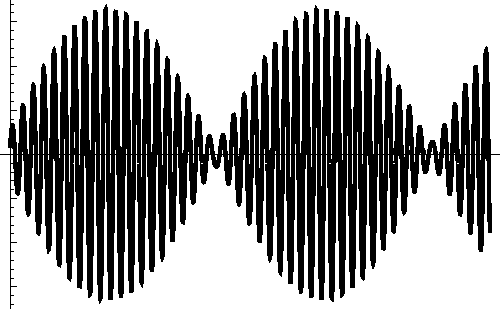
\includegraphics[width=\marginparwidth]{support/resonnance}
\\
Notice the beats. In this example, $\omega = 2$, $m=1.1$, $c\approx 0$, and $k=4$.  Since $\omega_0=\sqrt{4/1.1}\approx 2=\omega$, the solution results in large periodic oscillations. If the oscillations are too large, they will destroy the system.
}}%
Let's attach a mass-spring system to a wheel. Suppose $m=1$ and $k=4$ (with no dashpot). 
The driving force, $r(t)$, is periodic. 
\begin{enumerate}
 \item Assume the driving force is $r(t) = 7\sin(5t)$. Solve the IVP $y''+4y=7\sin(5t)$, where $y(0)=0$ and $y'(0)=0$. 
 \item
Assume $m$ and $k$ are known constants, and the driving force is $r(t) = F\sin(\omega t)$, where $\omega\neq \sqrt{k/m}$. Solve the IVP $my''+ky=F\sin(\omega t)$, where $y(0)=0$ and $y'(0)=0$.
\end{enumerate}
\end{problem}


\begin{problem}
\marginpar{{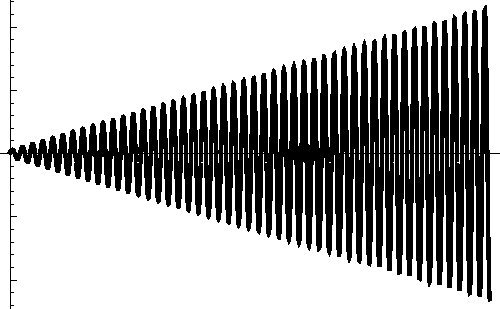
\includegraphics[width=\marginparwidth]{support/growing-oscillation}
\\
When $\omega_0=\omega$ and friction is negligible, a system will oscillate with an amplitude that grows without bound. Beware of this situation, as any mechanical system which undergoes this kind of oscillation will self destruct. 
}}%
Again, let's attach a mass-spring system to a wheel. Suppose $m=1$ and $k=4$ (with no dashpot). 
The driving force, $r(t)$, is periodic. 
\begin{enumerate}
 \item Assume the driving force is $r(t) =7 \sin(2t)$. Solve the IVP $y''+4y=7\sin(2t)$, where $y(0)=0$ and $y'(0)=0$. 
 \item Assume $m$ and $k$ are now some constant, and the driving force is $r(t) = A\sin(\omega t)$, where $\omega = \sqrt{k/m}$. Solve the IVP $my''+ky=F\sin(\omega t)$, where $y(0)=0$ and $y'(0)=0$.
\end{enumerate}
\end{problem}

Make sure you ask me in class to graph your two solutions above in Mathematica. The plots get interesting when $\omega\approx \sqrt{k/m}$, and the solution produces steady beats. You should see a rhythmic rise and fall in the amplitude of the solution.  When $\omega =  \sqrt{k/m}$, the solution grows without bound. The following YouTube videos show the collapse of the Tacoma Narrows bridge, and airplane flutter. The points to these videos is to show you the dangerous things that can (and do) happen to a structure when the designer forgets to take into account how external driving forces might interact with the internal frequencies of the mechanical system.
\begin{itemize}
 \item \href{http://www.youtube.com/watch?v=xox9BVSu7Ok}{The Tacoma Narrows bridge collapses.}
 \item \href{http://www.youtube.com/watch?v=iTFZNrTYp3k}{The tail of a small airplane begins to flutter.}
 \item \href{http://www.youtube.com/watch?v=OhwLojNerMU}{Watch a collection of flutter examples.}
 \item \href{http://www.youtube.com/watch?v=lczhD2nUedY}{An RC airplane looses its wing midflight.}
\end{itemize}

In both problems above, we assumed there was no friction ($c=0$).  Can we produce beats or resonance when there is friction? Let's analyze this problem and show that YES, bad things can still happen when friction is involved. To discover when disaster might occur, we have to work with symbolic answers and then ask, ``What would it take to produce large oscillations?''  Let's analyze this first with some specific numbers (to notice patterns) and then we'll analyze what happens symbolically.
\begin{problem}
Consider the ODE $y''+2y'+5y=5\sin(3 t)$.
\begin{enumerate}
 \item Find a general solution to this ODE.  
\WA{http://www.wolframalpha.com/input/?i=y\%27\%27\%2B2y\%27\%2B5y\%3D5\%5Csin\%283+t\%29}
 \item As $t$ increases, what happens to the homogeneous solution?
 \item If $y(0)=0$ and $y'(0)=0$, solve the IVP.
\end{enumerate}
\end{problem}

When friction enters a mass spring system, the homogeneous solution will always die out over time. The particular solution $y_p$ is called the ``steady-state'', or ``steady periodic'' solution. As time moves on, friction will damp out all oscillation except for the steady-state solution, $y_p$.  

\begin{problem}
Consider the ODE $my''+cy'+ky=F\sin(\omega t)$.
\begin{enumerate}
 \item What are the roots of the characteristic polynomial?
 \item We guess the steady-state solution (particular solution) is $y_p=A\cos(\omega t)+B\sin(\omega t)$.  Why do we never have to multiply the guess by $t$?
 \item Find the steady-state solution. As a hint, you'll probably find Cramer's Rule useful when solving for $A$ and $B$ (because you'll get a linear system with variables as coefficients). 
\WA{http://www.wolframalpha.com/input/?i=m+y\%27\%27\%28t\%29\%2Bc+y\%27\%28t\%29\%2Bk+y\%28t\%29\%3DF+\%5Csin\%28w+t\%29}
\end{enumerate}
 In class, we'll examine what it would take to get a really large amplitude for the steady-state solution (thus destroying the mechanical system).
\end{problem}
  

\subsection{Electric circuits} 
Remember that Kirchoff's voltage law states that the voltage (electromotive force) impressed on a closed loop is equal to the sum of the voltage drops across the other elements of the loop. We've summarized this by saying ``voltage in equals voltage out.'' Because we've been using complex numbers in our work, we'll use $I(t)$ to represent the current in a loop instead of $i(t)$. We've already used Kirchoff's voltage law in connection with resistors. Let's now add an inductor and a capacitor to a single loop. Each element (resistor, inductor, capacitor) produces the voltage drop given in the table below.
\begin{center}
\begin{tabular}{|l|l|l|}
\hline
Component & Voltage drop & Other\\\hline
Resistor & $RI$ & Ohm's law, where $R$ is in ohms\\\hline
Inductor & $LI' = L(dI/dt)$ & $L$ is in henrys\\\hline
Capacitor& $\dfrac{Q}{C} = \frac{1}{C}\frac{dI}{dt}$ & $Q$ is in coulombs, $C$ in farads.\\\hline
\end{tabular}
\end{center}
The charge $Q$ on a capacitor is related to the current by $I(t)=\frac{dQ}{dt}$, or $Q=\int I(t) dt$. 

We'll be studying $RC$, $RLC$, and $RL$ circuits in the next few chapters.  Table \ref{circuit table} shows the differential equations corresponding to each type of circuit.


\begin{table}[h]
\begin{center}
\begin{tabular}{ccc}
\renewcommand{\myscale}{.3}
\begin{tikzpicture}[scale=\myscale,inner sep=1pt]
%\draw[help lines,step=1cm] (0,0) grid (12,6);

%Source - like a battery
\node[label=right:$E$] at (0,3) 
{{\begin{tikzpicture}[scale=\myscale]
%	\useasboundingbox (-.5,-3) rectangle (.5,3);
	\draw (0,0) circle (1cm);
	\draw (.3,.5) -- (-.3,.5);
	\draw (0,.2) -- (0,.8);
	\draw (.3,-.5) -- (-.3,-.5);
	\draw (0,1) -- (0,3);
	\draw (0,-1) -- (0,-3);
	\end{tikzpicture}
}};

%Resistor
\node[label=right:$R$] at (6,3) 
{{\begin{tikzpicture}[scale=\myscale]
%	\useasboundingbox (0,-3) rectangle (0,3);
	\draw (0,-3) -- ++(0,1.8) -- ++(.5,.2) 
		-- ++(-1,.4) -- ++(1,.4)
		-- ++(-1,.4) -- ++(1,.4)
		-- ++(-1,.4) -- ++(.5,.2)
		-- ++(0,1.8) ;
	\end{tikzpicture}
}};

%Straight Path
%\node at (3,6) 
%{{\begin{tikzpicture}[scale=\myscale,rotate=90]
%	\draw (0,-3) -- (0,3);
%	\end{tikzpicture}
%}};

%Arrow to represent Current
\node[label=right:$i$] at (0,5) 
{{\begin{tikzpicture}[scale=\myscale,rotate=0]
	\filldraw (0,.4) -- (-.2,-.4) -- (0,-.3) -- (.2,-.4);
	\end{tikzpicture}
}};

%Loops
\node[label=above:$L$] at (3,6) 
{{\begin{tikzpicture}[scale=\myscale,rotate=90]
	\useasboundingbox (-.5,-3) rectangle (.5,3);
	\draw (0,-3) -- ++(0,1.5) 
	.. controls+(15:.2) and +(-90:.25) .. ++(.5,.4) 
	.. controls+(90:.25) and +(-15:.2) .. ++(-.5,.4) 
	.. controls+(-15:-.2) and +(90:.1) .. ++(-.5,-.05) 
	.. controls+(-90:.1) and +(15:-.2) .. ++(.5,-.05) 
	.. controls+(15:.2) and +(-90:.25) .. ++(.5,.4) 
	.. controls+(90:.25) and +(-15:.2) .. ++(-.5,.4) 
	.. controls+(-15:-.2) and +(90:.1) .. ++(-.5,-.05) 
	.. controls+(-90:.1) and +(15:-.2) .. ++(.5,-.05) 
	.. controls+(15:.2) and +(-90:.25) .. ++(.5,.4) 
	.. controls+(90:.25) and +(-15:.2) .. ++(-.5,.4) 
	.. controls+(-15:-.2) and +(90:.1) .. ++(-.5,-.05) 
	.. controls+(-90:.1) and +(15:-.2) .. ++(.5,-.05) 
	.. controls+(15:.2) and +(-90:.25) .. ++(.5,.4) 
	.. controls+(90:.25) and +(-15:.2) .. ++(-.5,.4) 
	-- (0,3);
	\end{tikzpicture}
}};


%Capacitor
\node[label=above:$C$] at (3,0) 
{{\begin{tikzpicture}[scale=\myscale,rotate=90]
%	\useasboundingbox (0,-3) rectangle (0,3);
	\draw (0,-3) -- ++(0,2.8) 
		-- ++(.5,0) -- ++(-1,0) 
		++(0,.4) -- ++(1,0)
		-- ++(-.5,0) -- ++(0,2.8);
	\end{tikzpicture}
}};


\end{tikzpicture}

&
\renewcommand{\myscale}{.3}
\begin{tikzpicture}[scale=\myscale,inner sep=1pt]
%\draw[help lines,step=1cm] (0,0) grid (12,6);

%Source - like a battery
\node[label=right:$E$] at (0,3) 
{{\begin{tikzpicture}[scale=\myscale]
%	\useasboundingbox (-.5,-3) rectangle (.5,3);
	\draw (0,0) circle (1cm);
	\draw (.3,.5) -- (-.3,.5);
	\draw (0,.2) -- (0,.8);
	\draw (.3,-.5) -- (-.3,-.5);
	\draw (0,1) -- (0,3);
	\draw (0,-1) -- (0,-3);
	\end{tikzpicture}
}};

%Resistor
\node[label=right:$R$] at (6,3) 
{{\begin{tikzpicture}[scale=\myscale]
%	\useasboundingbox (0,-3) rectangle (0,3);
	\draw (0,-3) -- ++(0,1.8) -- ++(.5,.2) 
		-- ++(-1,.4) -- ++(1,.4)
		-- ++(-1,.4) -- ++(1,.4)
		-- ++(-1,.4) -- ++(.5,.2)
		-- ++(0,1.8) ;
	\end{tikzpicture}
}};

%Straight Path
\node at (3,6) 
{{\begin{tikzpicture}[scale=\myscale,rotate=90]
	\draw (0,-3) -- (0,3);
	\end{tikzpicture}
}};

%Arrow to represent Current
\node[label=above:$i$] at (3,6) 
{{\begin{tikzpicture}[scale=\myscale,rotate=-90]
	\filldraw (0,.4) -- (-.2,-.4) -- (0,-.3) -- (.2,-.4);
	\end{tikzpicture}
}};

%Inductor
%\node[label=above:$L$] at (3,6) 
%{{\begin{tikzpicture}[scale=\myscale,rotate=90]
%	\useasboundingbox (-.5,-3) rectangle (.5,3);
%	\draw (0,-3) -- ++(0,1.5) 
%	.. controls+(15:.2) and +(-90:.25) .. ++(.5,.4) 
%	.. controls+(90:.25) and +(-15:.2) .. ++(-.5,.4) 
%	.. controls+(-15:-.2) and +(90:.1) .. ++(-.5,-.05) 
%	.. controls+(-90:.1) and +(15:-.2) .. ++(.5,-.05) 
%	.. controls+(15:.2) and +(-90:.25) .. ++(.5,.4) 
%	.. controls+(90:.25) and +(-15:.2) .. ++(-.5,.4) 
%	.. controls+(-15:-.2) and +(90:.1) .. ++(-.5,-.05) 
%	.. controls+(-90:.1) and +(15:-.2) .. ++(.5,-.05) 
%	.. controls+(15:.2) and +(-90:.25) .. ++(.5,.4) 
%	.. controls+(90:.25) and +(-15:.2) .. ++(-.5,.4) 
%	.. controls+(-15:-.2) and +(90:.1) .. ++(-.5,-.05) 
%	.. controls+(-90:.1) and +(15:-.2) .. ++(.5,-.05) 
%	.. controls+(15:.2) and +(-90:.25) .. ++(.5,.4) 
%	.. controls+(90:.25) and +(-15:.2) .. ++(-.5,.4) 
%	-- (0,3);
%	\end{tikzpicture}
%}};


%Capacitor
\node[label=above:$C$] at (3,0) 
{{\begin{tikzpicture}[scale=\myscale,rotate=90]
%	\useasboundingbox (0,-3) rectangle (0,3);
	\draw (0,-3) -- ++(0,2.8) 
		-- ++(.5,0) -- ++(-1,0) 
		++(0,.4) -- ++(1,0)
		-- ++(-.5,0) -- ++(0,2.8);
	\end{tikzpicture}
}};


\end{tikzpicture}

& 
\renewcommand{\myscale}{.3}
\begin{tikzpicture}[scale=\myscale,inner sep=1pt]
%\draw[help lines,step=1cm] (0,0) grid (12,6);

%Source - like a battery
\node[label=right:$E$] at (0,3) 
{{\begin{tikzpicture}[scale=\myscale]
%	\useasboundingbox (-.5,-3) rectangle (.5,3);
	\draw (0,0) circle (1cm);
	\draw (.3,.5) -- (-.3,.5);
	\draw (0,.2) -- (0,.8);
	\draw (.3,-.5) -- (-.3,-.5);
	\draw (0,1) -- (0,3);
	\draw (0,-1) -- (0,-3);
	\end{tikzpicture}
}};

%Resistor
\node[label=right:$R$] at (6,3) 
{{\begin{tikzpicture}[scale=\myscale]
%	\useasboundingbox (0,-3) rectangle (0,3);
	\draw (0,-3) -- ++(0,1.8) -- ++(.5,.2) 
		-- ++(-1,.4) -- ++(1,.4)
		-- ++(-1,.4) -- ++(1,.4)
		-- ++(-1,.4) -- ++(.5,.2)
		-- ++(0,1.8) ;
	\end{tikzpicture}
}};

%Straight Path
\node at (3,0) 
{{\begin{tikzpicture}[scale=\myscale,rotate=90]
	\draw (0,-3) -- (0,3);
	\end{tikzpicture}
}};

%Arrow to represent Current
\node[label=above:$i$] at (3,0) 
{{\begin{tikzpicture}[scale=\myscale,rotate=90]
	\filldraw (0,.4) -- (-.2,-.4) -- (0,-.3) -- (.2,-.4);
	\end{tikzpicture}
}};

%Inductor
\node[label=above:$L$] at (3,6) 
{{\begin{tikzpicture}[scale=\myscale,rotate=90]
	\useasboundingbox (-.5,-3) rectangle (.5,3);
	\draw (0,-3) -- ++(0,1.5) 
	.. controls+(15:.2) and +(-90:.25) .. ++(.5,.4) 
	.. controls+(90:.25) and +(-15:.2) .. ++(-.5,.4) 
	.. controls+(-15:-.2) and +(90:.1) .. ++(-.5,-.05) 
	.. controls+(-90:.1) and +(15:-.2) .. ++(.5,-.05) 
	.. controls+(15:.2) and +(-90:.25) .. ++(.5,.4) 
	.. controls+(90:.25) and +(-15:.2) .. ++(-.5,.4) 
	.. controls+(-15:-.2) and +(90:.1) .. ++(-.5,-.05) 
	.. controls+(-90:.1) and +(15:-.2) .. ++(.5,-.05) 
	.. controls+(15:.2) and +(-90:.25) .. ++(.5,.4) 
	.. controls+(90:.25) and +(-15:.2) .. ++(-.5,.4) 
	.. controls+(-15:-.2) and +(90:.1) .. ++(-.5,-.05) 
	.. controls+(-90:.1) and +(15:-.2) .. ++(.5,-.05) 
	.. controls+(15:.2) and +(-90:.25) .. ++(.5,.4) 
	.. controls+(90:.25) and +(-15:.2) .. ++(-.5,.4) 
	-- (0,3);
	\end{tikzpicture}
}};


%Capacitor
%\node[label=above:$C$] at (3,0) 
%{{\begin{tikzpicture}[scale=\myscale,rotate=90]
%	\draw (0,-3) -- ++(0,2.8) 
%		-- ++(.5,0) -- ++(-1,0) 
%		++(0,.4) -- ++(1,0)
%		-- ++(-.5,0) -- ++(0,2.8)
%	\end{tikzpicture}
%}};


\end{tikzpicture}

\\
An $RLC$-circuit
&An $RC$-circuit
&An $RL$-circuit
\\\hline
$L I'+ RI+ \frac{1}{C}\int I(t) dt = E(t)$
&$RI+ \frac{1}{C}\int I(t) dt = E(t)$
&$L I'+ RI = E(t)$
\\
$L Q''+ RQ'+ \frac{1}{C}Q = E(t)$
&$RQ'+ \frac{1}{C}Q = E(t)$
&%$L Q''+ RQ' = E(t)$
\\
$L I''+ RI'+ \frac{1}{C}I = E'(t)$
&$RI'+ \frac{1}{C}I = E'(t)$
&%$L I''+ RI' = E'(t)$
\\\hline
\end{tabular}
\end{center}
\caption{Typical diagrams of $RCL$, $RC$, and $RL$ circuits, and their corresponding ODEs. The first row is an integro-differential equation for the current $I(t)$. The second row is the ODE for the charge $Q$ on the capacitor. The third row is the derivative of the first row. \label{circuit table}
}
\end{table}

In a circuit  with one resistor, one inductor, and one capacitor (an $RLC$ circuit), if the electromotive force is $E(t)$, then Kirchoff's Voltage law gives the integro-differential equation 
$$L I'+ RI+ \frac{1}{C}Q(t) =E(t) \quad \text{or}\quad L I'+ RI+ \frac{1}{C}\int I(t) dt = E(t).$$  
Differentiating both sides removes the integral and gives
$$L I''+ RI'+ \frac{1}{C}I(t) = E'(t),$$ which is a second order linear differential equation with constant coefficients. However, the initial conditions are in terms of initial charge $Q(0)$ and initial current $I(0)$. To solve the differential equation for $I$, we need $I'(0)$, which we can get from the equation $ L I'(t)+ RI(t)+ \frac{1}{C}Q(t) =E(t)$. Problem 14.13 in Schaum's provides an excellent example that summarizes the solution technique.
 
\begin{problem}
Consider an $RLC$ circuit with $L=1/2$, $R=2$, and $C=2/3$. Let's plug the circuit into an alternating current power source (like a wall outlet), which means we might have something like $E(t) = 2\cos(3t)$.  Initially, assume that the current is zero and the charge on the capacitor is zero. We'd like to find the current at any time $t$ in the circuit.
\begin{enumerate}
 \item Explain why the current satisfies $I''+4I'+3I=-12\sin(3t)$. Find a general solution to this ODE.
\WA{http://www.wolframalpha.com/input/?i=y\%27\%27\%2B4y\%27\%2B3y\%3D-12\%5Csin\%283t\%29}
 \item We know that $I(0)=0$ and $Q(0)=0$.  Use the equation $L I'(t)+ RI(t)+ \frac{1}{C}Q(t) =E(t)$ to explain why $I'(0) = 4$. 
 \item Find the current in the wire at any time $t$ by solving the corresponding IVP. Use the initial conditions you found in the previous part.
\WA{http://www.wolframalpha.com/input/?i=y\%27\%27\%2B4y\%27\%2B3y\%3D-12\%5Csin\%283t\%29\%2C+y\%280\%29\%3D0\%2C+y\%27\%280\%29\%3D4}
 \item What is the steady-state current? (Which part of your solution above does not vanish after sufficient time has passed? This would be the current flowing through the circuit after the initial conditions have died out.)
\end{enumerate}
\end{problem}

\begin{problem}
Consider an $RLC$ circuit with $L=1$, $R=8$, and $C=\frac{1}{25}$. Let's plug the circuit into a 12 V battery, so we have $E(t) =12$.  Initially, assume that the current is zero and the charge on the capacitor is zero. We'd like to find the current at any time $t$ in the circuit.
\begin{enumerate}
 \item State the IVP whose solution would give the current at any time $t$. (What's the ODE, and what are the initial conditions $I(0)$ and $I'(0)$).  [Hint: Use the equation $L I'(t)+ RI(t)+ \frac{1}{C}Q(t) =E(t)$ to find $I'(0)$.] 
 \item Find the current in the wire at any time $t$. Check your answer with WolframAlpha (you'll want to use $y$ instead of $I$).
 \item What's the steady-state current?
\end{enumerate}

\end{problem}

\begin{observation}
Mechanical models are expensive to build.  Electrical models are fairly simple to build and measure.  If you need to create a mechanical system, it may prove beneficial financially to start with an electrical model. Engineers spend another semester on this idea in system dynamics.  Hydraulic systems are also very closely related. In bridging between mechanical and electrical systems, we compare the following variables. 
\begin{center}
\begin{tabular}{|c|c|c|c|c|c|}
\hline
Mechanical System&$m$&$c$&$k$&$r(t)=F_0\cos\omega t$&$y(t)$\\\hline
Electrical System&$L$&$R$&$1/C$&$E'(t) = E_0\omega\cos\omega t$&$I(t)$\\
\hline
\end{tabular}
\end{center}
Solving a problem in one system (either mechanical or electrical) can provide useful results in the other.  
\end{observation}



\section*{Wrap up}
\addcontentsline{toc}{section}{Wrap Up}

This concludes the chapter.  Look at the objectives at the beginning of the chapter. Can you now do all the things you were promised? 


\begin{problem}[Lesson Plan Creation] \marginpar{This counts as 4 prep problems. My hope is that you spend at least an hour creating your one-page lesson plan.}
Your assignment: organize what you've learned into a small collection of examples that illustrates the key concepts. I'll call this your one-page lesson plan. You may use both sides. The objectives at the beginning of the chapter give you a list of the key concepts. Once you finish your lesson plan, scan it into a PDF document (use any scanner on campus), and then upload the document to I-Learn.
\end{problem}






\newgeometry{left=1in,right=1in,top=1in,bottom=1in}

\section*{Extra Practice}
\addcontentsline{toc}{section}{Extra Practice}

The problems below come from Schaum's Outlines \textit{Differential Equations} by Richard Bronson. If you are struggling with a topic from the preparation problem set, please use this list as a guideline to find related practice problems.

\begin{center}
\begin{tabular}{|l|c|l|l|l|l|}
\hline
Concept&Sec&Suggestions&Relevant Problems\\ \hline
Theory&8&21,65&21-23,65-67\\ \hline
Undetermined Coef&11&1,2,3,8,10,24,26,34,36,41,46,47,48&All\\ \hline
IVP&13&1,7,14&1,3,7,8,10,11,14\\ \hline
Applications&7&19,76&19-22,71-81\\ \hline
Applications&14&10,11,13,14,17,46,50,51,52,54,57&9-18,44-65\\ \hline
\end{tabular}
\end{center}


Remember that you can check almost all of your work with technology. Wolfram Alpha provides a great resource for rapidly checking your work in this chapter.
% \begin{itemize}
%  \item Links are coming.
%  \item Links are coming.
% \end{itemize}


\restoregeometry




\chapter{Laplace Transforms}
\newcommand{\urlmathematicatechintro}{https://content.byui.edu/file/664390b8-e9cc-43a4-9f3c-70362f8b9735/1/_zips/316-Tech-Introduction.zip}

After completing this chapter, you should be able to:

\begin{enumerate}
\item Explain how to compute Laplace transforms and inverse Laplace transforms. Use Laplace transforms to solve IVPs.

\item Use and prove both both the $s$-shifting and $t$-shifting theorems. 
\item Express discontinuous functions with the Heaviside function, and use the Heaviside to set up and solve ODEs.
\item Express impulses in terms of the Dirac delta distribution, and use it to set up and solve solve ODEs.
\item Compute convolutions, and show how to use the convolution theorem as an inverse product rule for Laplace transforms.
\end{enumerate}

\marginpar{You may want to download this \href{\urlmathematicatechintro}{Mathematica Technology Introduction} to check your work throughout the entire chapter.}%
You can find additional practice problems in Schaum's Outlines \textit{Differential Equations} by Richard Bronson.
You'll find relevant problems in chapters 21 -24, as well as some extra practice problems at the end of this chapter. 
Do enough of each type that you feel comfortable with the ideas. 

\begin{table}[h]
\begin{center}
\begin{tabular}{cc}
\begin{tabular}[t]{|c|cc|}
\hline
$f(t)$ & $F(s)$ & provided\\
\hline\hline
$1$					&$\dfrac{1}{s}$ 							&$s>0$\\\hline
$t^n$				&$\dfrac{n!}{s^{n+1}}$ 			&$s>0$\\\hline
$e^{at}$		&$\dfrac{1}{s-a}$ 			&$s>a$\\\hline
$y'$					&$sY-y(0)$ 						&\\\hline
$y''$					&$s^2Y-sy(0)-y'(0)$ 						&\\\hline
%$y'''$					&$s^3Y-s^2y(0)-sy'(0)-y''(0)$ 						&\\\hline
$e^{at}f(t)$  &$F(s-a)$ 						&\\\hline
$f(t)*g(t)$  &$F(s)G(s)$ 						&\\\hline
\end{tabular}
&
\begin{tabular}[t]{|c|cc|}
\hline
$f(t)$ & $F(s)$ & provided\\
\hline\hline
$\cos(wt)$  &$\dfrac{s}{s^2+\omega^2}$ 			&$s>0$\\\hline
$\sin(wt)$  &$\dfrac{\omega}{s^2+\omega^2}$ 			&$s>0$\\\hline
$\cosh(wt)$ &$\dfrac{s}{s^2-\omega^2}$ 			&$s>|\omega|$\\\hline
$\sinh(wt)$ &$\dfrac{\omega}{s^2-\omega^2}$ 			&$s>|\omega|$\\\hline
$u(t-a)$  &$\frac{1}{s}e^{-as}$ 						&\\\hline
$\delta(t-a)$  &$e^{-as}$ 						&\\\hline
$f(t-a)u(t-a)$  &$\mathscr{L}(f(t))e^{-as}$ 						&\\
$f(t)u(t-a)$  &$\mathscr{L}(f(t+a))e^{-as}$ 						&\\
\hline
\end{tabular}
\end{tabular}
\end{center}
\caption{Table of Laplace Transforms\label{big laplace table}. Note that the $s$ shifting theorem $\mathscr{L}(e^{at}f(t))=F(s-a)$ has a positive $a$ in the exponent, while the $t$ shifting theorem $\mathscr{L}(f(t-a)u(t-a))=\mathscr{L}(f(t))e^{-as}$ has a negative $a$ in the exponent.
}
\end{table}


You must practice lots of problems to gain a feel for patterns.  Many of the problems in 21-23 are fast. Please take a few minutes every day to just flat out practice with the basics (kind of like when you were learning the times tables - they get really fast if you just practice them). When you feel like you have the basics down, see if you can complete chapters 21 and 22 in less than an hour. If one stumps you, skip it and come back later.  

Once you feel confident, chapters 23 (on convolutions and the heaviside function) and 24 (solving IVPS) will help you use the Laplace transforms to solve ODEs. At the end of this chapter are some additional problems to help you cement your understanding. Table \ref{big laplace table} summarizes the transforms we use most often.




\newcommand{\ReviewSShiftTheorem}{

In this chapter we'll examine how to handle non differentiable changes in an external driving force.  This corresponds to hitting a mass-spring system with a hammer, marching across a bridge, flipping a switch in an electrical network, etc.  We'll find that Laplace transforms provide us with extremely nice tools to solve these types problems.  Before we jump in, let's review how to solve a couple ODEs with Laplace transforms, and perhaps make some connections that we haven't yet made. 

\begin{review*}
 Compute the inverse Laplace transform of $\ds 	\frac{3s+8}{(s+1)^2+16}$. See
\footnote{
We can rewrite $Y$ as 
$$Y 
= \frac{3(s+1)-3+8}{(s+1)^2-16}
= \frac{3(s+1)}{(s+1)^2-16}+\frac{5}{(s+1)^2-16}\frac44.
$$
The inverse Laplace transform is then 
$$y(t) = 3e^{-t}\cosh(4t)+\frac{5}{4}e^{-t}\sinh(4t).$$
}.
\end{review*}







\begin{problem}\label{review of s-shifting theorem}
\marginpar{We've solved inverse transforms such as this one multiple times. If you need to refresh, please head to chapters 21 and 22 in Schaum's, and just practice the problems where answers are provided.}%
 Compute the inverse Laplace transform of $$\ds Y =\frac{5}{(s+3)^3} + \frac{2s+3}{(s+4)^2+9} + \frac{3s+1}{(s+2)^2-49}.$$ 
Use the rules for $\cosh(t)$ and $\sinh(t)$ to tackle the last terms, rather than doing a partial fraction decomposition.  The goal of this problem is to make sure you have the $s$-shifting theorem mastered.
%See 
% \footnote{We have
% $$\begin{array}{rl}
% \ds Y 
% &=\frac{5}{(s+3)^3} + \frac{2(s+4)-8+3}{(s+4)^2+9} + \frac{3(s+2)-6+1}{(s+2)^2-49}\\ 
% &=\frac{5}{(s+3)^3}\frac{2}{2} + \frac{2(s+4)}{(s+4)^2+9} +\frac{-5}{(s+4)^2+9}\frac{3}{3} + \frac{3(s+2)}{(s+2)^2-49}+ \frac{-5}{(s+2)^2-49}\frac{7}{7} 
% \end{array}$$
% The inverse transform is 
% $$\ds y(t) 
% = \frac{5}{2} t^2e^{-3t} 
%  + 2e^{-4t}\cos(3t) 
%  +\frac{-5}{3}e^{-4t}\sin(3t) 
%  +3 e^{-2t}\cosh(7t)
%  +\frac{-5}{7} e^{-2t}\sinh(7t).
% $$
% }.
\end{problem}
}



\newcommand{\CompareDistinctRootsToCoshAndSinh}{
\begin{problem}\label{compare distinct roots with s-shifting and cosh and sinh}
 Consider the IVP $y''+6y'+8y = 0$, $y(0)=2$, $y'(0)=3$.
\begin{enumerate}
 \item Use Laplace transforms to solve the IVP. Use a partial fraction decomposition to write $Y = \frac{A}{s+2}+\frac{B}{S+4}$ and then show that $\ds y(t) = \frac{11}{2}e^{-2t}-\frac{7}{2}e^{-4t}$.  
 \item Instead of using a partial fraction decomposition, instead notice that we could complete the square in the denomoinator to write $s^2+6s+8=(s+3)^2-1$. Use this approach to solve for $y(t)$ and write $y(t)$ as a linear combination of $e^{-3t}\cosh(t)$ and $e^{-3t}\sinh(t)$.
 \item Remember that $\ds \cosh(t) = \frac{e^t+e^{-t}}{2}$ and $\ds \sinh(t) = \frac{e^t-e^{-t}}{2}$. Use this to show how your second solution involving hyperbolic trig functions is really the same as $\ds y(t) = \frac{11}{2}e^{-2t}-\frac{7}{2}e^{-4t}$.
\end{enumerate}
\end{problem}

}

\newcommand{\ExtraCompareDistinctRootsToCoshAndSinh}{
\begin{problem}\label{extra compare distinct roots with s-shifting and cosh and sinh}
 Consider the IVP $y''+7y'+10y = 0$, $y(0)=4$, $y'(0)=-3$.
\begin{enumerate}
 \item Use Laplace transforms and a partial fraction decomposition to solve the IVP. Write your answer as a linear combination of $e^{-2t}$ and $e^{-5t}$.  
 \item Complete the square on $s^2+7s+10$ and use the Laplace transform with $\cosh$ and $\sinh$ rules to solve the IVP.
 \item Which is easier?
\end{enumerate}
\end{problem}

Problems 
\ref{compare distinct roots with s-shifting and cosh and sinh}
and 
\ref{extra compare distinct roots with s-shifting and cosh and sinh}
reviewed the main ideas used in solving ODEs with Laplace transforms.  In addition, these problems illustrate some of the advantages of using the hyperbolic trigonometric functions $\cosh\omega t$ and $\sinh\omega t$. They can greatly simplify computations.

}




\newcommand{\RLCircuitWithBatteryInsertedAndRemovedUsingMovingInitialConditions}{
We can use Laplace transforms to obtain quick solutions to problems with discontinuous external forces. Let's start by examining an $RL$ circuit with a battery, because it keeps the computations simple.

\begin{problem}\label{RLCircuitWithBatteryInsertedAndRemovedUsingMovingInitialConditions}
 Consider an $RL$ circuit with $R=1$ ohms and $L=1$ Henry.  At time zero, there is no battery in the system.  After 2 seconds,  we connect a battery $E=12 V$ to the circuit.  Two seconds after connecting the battery, we disconnect it.  Our goal is to determine the current in the wire exactly 2 second after we disconnect the battery.
\begin{enumerate}
 \item During the first  two seconds, we need to solve the IVP $I'+I=0$ where $I(0)=0$.  Solve this IVP and use your solution to show that the current after 2 seconds is $I(2)=0$.
 \item Between $t=2$ and $t=4$, we know $E=12$.  Solve the IVP $I'+I=12$, $I(2)=0$. Show that $I(4) = 12-12e^{-2}$. This is the current as the battery gets removed.
\WA{http://www.wolframalpha.com/input/?i=y\%27\%2By\%3D12\%2C+y\%282\%29\%3D0}
 \item When we remove the battery, the ODE is $I'+I=0$. We know the initial condition $I(4)=12-12e^{-2}$ from the previous part.  Solve the IVP, and state $I(6)$. 
 \item We can now predict the current at any time $t$. Use piecewise function notation to state the current in the form
$$I(t) = 
\begin{cases}
 0 & 0\leq t< 2\\
 12-12e^{2}e^{-t} & 2\leq t< 4\\
 ? & 4\leq t\\
\end{cases}
.$$ 
\end{enumerate}
\end{problem}

}


\newcommand{\RLCircuitWithBatteryInsertedAndRemovedUsingShifting}{
In Problem \ref{RLCircuitWithBatteryInsertedAndRemovedUsingMovingInitialConditions}, we found the current using the initial conditions $I(0)=0$, $I(2)=0$, and $I(4)=?$. Another way to tackle this problem is to move our reference frame, letting $t=0$ correspond to the beginning of each change. The computations are often simpler, and we then just have to shift the reference frame back when we finish the problem. 

\begin{problem}\label{RLCircuitWithBatteryInsertedAndRemovedUsingShifting}
 Consider again the same $RL$ circuit with $R=1$ ohms and $L=1$ Henry.  At time zero, there is no battery in the system.  After 2 seconds,  we connect a battery $E=12 V$ to the circuit.  Two seconds after connecting the battery, we disconnect it.  Our goal is to determine the current in the wire exactly 2 second after we disconnect the battery. We'll solve this problem by always making $t=0$ the start of each IVP.
\begin{enumerate}
 \item During the first  two seconds, we need to solve the IVP $I'+I=0$ where $I(0)=0$.  Solve this IVP and use your solution to show that the current after 2 seconds is $I(2)=0$.
 \item Between 2 and 4 seconds, we know $E=12$. Letting $t=0$ correspond to 2 seconds, solve the IVP $I'+I=12$, $I(0)=0$. What is $I(2)$, the current right when the battery gets removed?
 \item When we remove the battery, the ODE is $I'+I=0$. Let $t=0$ correspond to 4 seconds, and then we know the initial condition $I(0)$ from the last part.  Solve the IVP, and state the current $I(2)$ after 6 seconds. 
 \item Use piecewise function notation to state the current at any time $t$. Remember to shift your solutions from the 2nd and 3rd part. Your answer will look like 
$$I(t) = 
\begin{cases}
 0 & 0\leq t< 2\\
 12-12e^{-(t-2)} & 2\leq t< 4\\
 ? & 4\leq t\\
\end{cases}
.$$ 
\end{enumerate}
\end{problem}

}








\newcommand{\IntroductionToGraphingPiecewiseDefineFunctions}{
The electromotive force $E(t)$ in Problem \ref{RLCircuitWithBatteryInsertedAndRemovedUsingMovingInitialConditions} was a piecewise defined force. It was zero, then 12, then 0. Using piecewise notation, we would write this as
$$E(t) =
\begin{cases}
 0 & 0\leq t<2\\
 12 & 2\leq t<4\\
 0 & 4\leq t
\end{cases}
,$$
and we could graph the function $E(t)$ using the figure to the right.
\marginpar{
\begin{tikzpicture}[scale=.5]
%\draw[step=1cm,gray,very thin,dashed] (-1,-1) grid (7,3);
\draw (-1,0) -- (7,0);
\draw (0,-1) -- (0,3);
\draw[very thick] (0,0) -- (2,0);
\draw[dashed] (2,0) -- (2,2);
\draw[very thick] (2,2) -- (4,2);
\draw[dashed] (4,2) -- (4,0);
\draw[very thick] (4,0) -- (7,0);
\end{tikzpicture}
}
We need a nice clean way to work with piecewise defined external forces.  We also need to become comfortable graphing and working with these kinds of forces.

\begin{problem}
% Give them a piecewise defined function, have them graph it.  Then give them a graph, and have them define the function.
Consider the functions 
$$
f(t) = 
\begin{cases}
 2t & 0\leq t< 2\\
 -t^2+4t & 2\leq t< 4\\
 18-3t& 4\leq t< 6\\
 t^2-12t+35& 6\leq t< 8
\end{cases}
\quad\text{and}
\quad
g(t) = 
\begin{cases}
 2t & 0\leq t< 2\\
 4-(t-2)^2 & 2\leq t< 4\\
 6-3(t-4)& 4\leq t< 6\\
 (t-6)^2-1& 6\leq t< 8
\end{cases}.
$$
\begin{enumerate}
 \item Graph $f(t)$ in the $ty$ plane. 
 \item Graph $g(t)$ in the $ty$ plane. 
 \item Graph $y=2t$, $y=4-t^2$, $y=6-3t$, and $y=t^2-1$ in the $ty$ plane.  What does this have to do with the above?
\end{enumerate}

\end{problem}

}



%\subsection{The Heaviside function $u(t-a)$}

\newcommand{\DefinitionOfHeavisideAndGraphOfAFewFunctions}{
We now define the key function that allows us to work with piecewise defined functions.  Some people call this the Heaviside function, some call it the unit step function. This is a simple function that jumps up a single unit at a specified value of $t$. 
\begin{definition}[Heaviside or Unit Step Function]
\marginpar{In our work, it won't matter what we define $u(0)$ to equal. Here, we define $u(0)=1$, but we could have just as easily define $u(0)=0$ or $u(0)=1/2$.  This last option, the 1/2, comes in handy when working with Fourier series.}
We define the Heaviside, or unit step function, to be the function
$$u(t) = \begin{cases}0 &t<0 \\ 1 &t\geq 0\end{cases}.$$ 
We'll most often shift this function right $a$ units, so we replace $t$ with $t-a$, which means we could write
$$u(t-a) = \begin{cases}0 &t-a<0 \\ 1 &t-a\geq 0\end{cases}\quad \quad \text{or}\quad u(t-a)= \begin{cases}0 &t<a \\ 1 &t\geq a\end{cases}.$$ 
\end{definition}
Why does this function matter.  It's like an on/off function.  If you multiply $f(t)$ by $u(t-a)$, then the function $f(t)u(t-a)$ is zero to the left of $a$, and is equal to $f(t)$ after $a$. If $a=3$, then look below for the graph of $y=u(t-3)$.
\marginpar{Mathematica uses the name ``HeavisideTheta'' for the Heaviside function.  You'll see the symbol $\theta$ show up as the name of a function. }
\begin{center}
\begin{tikzpicture}[xscale=1,yscale=1]
\draw[very thick,<-,gray] (-1,0)--(3,0);
\draw[very thick,->,gray] (3,1)--(8,1);
\draw[->,gray] (0,0)--(0,2);
\draw[->,gray] (0,0)--(0,-1);
\draw[->,gray] (0,0)--(-1,0);
\draw[->,gray] (0,0)--(9,0);
\foreach \x in {0,...,8}
	\draw[gray] (\x,4pt) -- (\x,-4pt);
\foreach \y in {0,...,1}
	\draw[gray] (2pt,\y) -- (-2pt,\y);
\path (5,1.5) node {$y=u(t-3)$};
\draw (3,0) circle (3pt);
\filldraw (3,1) circle (3pt);
\end{tikzpicture}  
\end{center}
  
\begin{problem}
 Construct a graph of each of the following:
\begin{enumerate}
 \item $f(t) = u(t-4) - u(t-7)$\marginpar{WolframAlpha and I are having issues when it comes to plotting Heavisides.  I can plot the first one just fine, but as soon as I times it by $(10-t)$, it tries to plot a surface.  As such, \href{http://aleph.sagemath.org/?z=eJwrSyzSUC9R1-RK0yjRtNUwNNAt0dTSyEhNLMsszkxJ1SjRNdHUReaaa2pycRXk5JdogHToaJToGOhYaGoCAP0RFH0=&lang=sage}{please use this link to Sage to check your work.} Make sure you can explain how the graphs are made (not just give them).}
 \item $g(t) = (10-t)(u(t-4) - u(t-7))$
 \item $h(t) = (10-(t-4))(u(t-4) - u(t-7))$ (How does this differ from the previous?)
 \item $k(t) = t^2 (u(t-3) - u(t-5))$
 \item $l(t) = (t-3)^2( u(t-3) - u(t-5))$ (How does this differ from the previous?)
\end{enumerate}
\href{http://aleph.sagemath.org/?z=eJwrSyzSUC9R1-RK0yjRtNUwNNAt0dTSyEhNLMsszkxJ1SjRNdHUReaaa2pycRXk5JdogHToaJToGOhYaGoCAP0RFH0=&lang=sage}{Make sure you check your solution by following the link to Sage.}
\end{problem}

}


\newcommand{\GettingFromAGraphToAHeavisideFunction}{
\begin{problem}
% I need something that would show them the reason for $t$ shifting.  Have them concatenate 3 graphs. Give them some crazy ugly thing that is TONS simpler if you first shift each piece.  Then graph it. 
The graphs of $f(t)=9-t^2$ for $0\leq t\leq3$, and $g(t)=3t$ for $0\leq t\leq 2$, and $h(t) = 6-2t$ for $0\leq t\leq 2$ are connected together (when one ends, the others starts) to give the following graph.
\begin{center}
\begin{tikzpicture}[xscale=.5,yscale=.2]
\draw plot[variable=\t,samples=20,domain=0:3] ({\t},{9-\t*\t});
\draw plot[variable=\t,samples=20,domain=3:5] ({\t},{3*(\t-3)});
\draw plot[variable=\t,samples=20,domain=5:8] ({\t},{6-2*(\t-5)});
\draw[->,gray] (0,0)--(0,10);
\draw[->,gray] (0,0)--(0,-1);
\draw[->,gray] (0,0)--(-1,0);
\draw[->,gray] (0,0)--(11,0);
\foreach \x in {-1,...,10}
	\draw[gray] (\x,4pt) -- (\x,-4pt);
\foreach \y in {-1,...,9}
	\draw[gray] (2pt,\y) -- (-2pt,\y);
\end{tikzpicture}  
\end{center}
\begin{enumerate}
 \item Write this function using piecewise function notation.
 \item Write this function using Heaviside notation. You'll want to use the idea that $u(t-a)-u(t-b)$ turns a function on at $a$ and off at $b$. 
 \item When you think you have the function, \href{http://aleph.sagemath.org/?z=eJwrSyzSUC9R1-RK0yjRtNUwNNAt0dTSyEhNLMsszkxJ1SjRNdHUReaaa2pycRXk5JdogHToaJToGOhYaGoCAP0RFH0=&lang=sage}{use this Sage link to check if you are correct} (you'll have to type in your function). 

 Feel free to use Mathematica instead, if you have downloaded and installed it.  Remember that BYU-I students can now install Mathematica on their personal machines for free. Please head to I-Learn for instructions.  You can then download this \href{https://content.byui.edu/file/664390b8-e9cc-43a4-9f3c-70362f8b9735/1/_zips/316-Tech-Introduction.zip}{Mathematica Technology Introduction}, and you'll see how to code HeavisideTheta functions in Mathematica. 
\end{enumerate}
\end{problem}

Did you notice in your work above that it was a lot easier to graph a piecewise defined function when everything was shifted to the starting point.  It's much easier to graph $f(t-a)u(t-a)$ than it is to graph $f(t)u(t-a)$.  We'll find that this remains true as well, when we start applying Laplace transforms.  

}


\newcommand{\DevelopLaplaceTransformOfHeavisideFunction}{
It's time to look at the Laplace transform of the Heaviside function. This problem is the key to why Laplace transforms work so nicely with piecewise defined functions.  We'll compute the Laplace transform of both $f(t-a)u(t-a)$ and $f(t)u(t-a)$.  Then we'll practice on a few problems.

\begin{problem}[$t$-shifting Theorem]
 Suppose that $y=f(t)$ is a function for which you can find the Laplace transform.
\begin{enumerate}
 \item Show, using the definition of the Laplace transform, that we have
$$\mathscr{L}\{f(t-a)u(t-a)\} = \mathscr{L}\{f(t)\}e^{-as}.$$
 In particular, this means that $\mathscr{L}\{1u(t-a)\}=\frac{1}{s}e^{-as}$.  
\item Then show that
$$\mathscr{L}\{f(t)u(t-a)\} = \mathscr{L}\{f(t+a)\}e^{-as}.$$
\end{enumerate}
[Hint: For the first part, just write down the definition of the Laplace transform. You'll have to do a substitution $w=t-a$. Remember that $u(t-a)=0$ if you are below $a$, which should allow you to remove $u(t-a)$ from any integral, after updating the bounds. In particular, you know that $$\int_0^\infty e^{-st}f(t-a)u(t-a)dt=\int_0^a e^{-st}f(t-a)(0)dt+\int_a^\infty e^{-st}f(t-a)(1)dt = 0+\int_a^\infty e^{-st}f(t-a)dt.$$]
 
\end{problem}

}

\newcommand{\PracticeForwardLaplaceOfHeaviside}{
\begin{problem}
 Compute the Laplace transforms of each of the following functions. \marginpar{See Schaum's chapter 24 for lots more practice.  Please do a bunch of these until you feel like you have the idea down.  Each problem takes just a tiny bit of time. Unless you practice this a bunch, you'll be lost and spend gobs of time on the upcoming problems.}
 \begin{enumerate}
  \item $f(t) = 3u(t-4)$
  \item $f(t) = 3(t-4)\,u(t-4)$
  \item $f(t) = 3t\,u(t-4)$ [Hint: $3t=3(t-4)+12$]
  \item $f(t) = (t-3)^2u(t-3)$
  \item $f(t) = t^2(u(t-2)-u(t-5))$
 \end{enumerate}
\end{problem}

}

\newcommand{\PracticeInverseLaplaceOfHeaviside}{
\begin{problem}
 Compute the inverse Laplace transform of each of the following functions.
 \begin{enumerate}
\begin{multicols}{4}  \item $\dfrac{4}{s^3}e^{-2s}$
  \item $\dfrac{4}{(s+5)^3}e^{-2s}$
  \item $\dfrac{2s+1}{s^2+9}e^{-\pi s/6}$
  \item $\dfrac{3s+4}{(s+2)^2+16}e^{-5s}$
 \end{multicols}
 \end{enumerate}
\end{problem}

}


\newcommand{\FirstSimpleRLCircuitIVP}{
We are now ready to solve Laplace transform problems with the Heaviside function.  The simplest example is an $RL$ circuit.
\begin{problem}
 Consider an $RL$ circuit with $R=4$ and $L=1$. At $t=0$ there is no current in the wire.  Two seconds later ($t=2$), we connect a 9V battery to the circuit.  Three seconds later ($t=5$) we remove the battery.  This gives us the electromotive force as $E(t) = 9(u(t-2)-u(t-5))$.  
 We need to solve the IVP
 $$1I'+4I=9(u(t-2)-u(t-5)), \quad I(0)=0.$$
 Use Laplace transforms to predict the current $I(t)$ at any time $t$. Check your answer with technology. 
 [Hint: You'll want to ignore the $e^{-as}$ terms when you perform any needed partial fraction decompositions.]
\end{problem}

}


\newcommand{\RLCircuitWithRampUpForce}{
\begin{problem}
\marginpar{Remember that the key ODE is $LI'+RI+\frac{1}{C}Q=E$.  We only have to compute $E'$ if there is a capacitor in the problem.} Consider an $RL$ circuit with $R=5$ and $L=1$. We connect a variable voltage source to the circuit and start to ramp up the power.  Suppose our electromotive force is $E(t)=t$ volts. After 12 seconds, we loose power and $E(t)$ drops to zero. Solve for the current in the wire at any time $t$.

[Hint: The electromotive force is $E(t) = t - tu(t-12)$, which means we solve
$$I'+5I=t - tu(t-12), \quad I(0)=0.$$
Use Laplace transforms and the $t$-shifting theorem to complete this.]
\end{problem}

}

\newcommand{\MassSpringSystemPulledDownByAMagnet}{
\begin{problem}
 Consider a vertical mass spring system, where we attach a magnetic brick to the bottom of the spring. Let $y=0$ be the equilibrium height of the brick after accounting for gravity (so we can ignore the force of gravity). 
Suppose that $m = 1$, $c = 0$, and $k=4$. The spring is pushed upwards 1 unit, and then let go from rest. After 3 seconds, an electromagnet pulls down on the spring with a force of 7 (the units all agree). We can model this using $r(t)=-7u(t-3)$.  Solve the ODE $y''+4y=-7u(t-3)$. Check your solution with Mathematica or Sage. 
\end{problem}

}







\newcommand{\RocketInSpaceThroughJello}{
\begin{problem*}[Optional]
 We decide to launch a rocket.  We attach an engine to the rocket, and light it. Neglect the mass of the fuel.  The mass of the rocket and engine we'll assume is $4$ kg. Let's launch the rocket in space, so we can ignore the force due to gravity. \marginpar{Ask me in class to show you how to modify this to add in gravity, or come by and show me what you would do. It's a pretty fun switch.)} Since we are in space, we don't have air resistance, so instead let's assume that we've put some Jello out in space, and the rocket plans to fly through the Jello (something to slow it down). Assume that the force due to the Jello's resistance is proportional to the velocity of the rocket, with proportionality constant $8$ kg/s.  When we light the engine, for the first 2 seconds the force ramps up, following a linear path until it gives a force of $10$ N after 2 seconds.  Then for 15 more seconds the rocket maintains a force of $10$ N.  The force then starts to ramp down linearly, taking an additional 5 seconds until the force drops to zero. A picture of this force is below.
\begin{center}
\begin{tikzpicture}[xscale=.2,yscale=.2]
\draw plot[variable=\t,samples=20,domain=0:2] ({\t},{5*\t});
\draw plot[variable=\t,samples=20,domain=2:17] ({\t},{10});
\draw plot[variable=\t,samples=20,domain=17:22] ({\t},{10-2*(\t-17)});
\draw[->,gray] (0,0)--(0,11);
\draw[->,gray] (0,0)--(0,-1);
\draw[->,gray] (0,0)--(-1,0);
\draw[->,gray] (0,0)--(23,0);
\foreach \x in {-1,...,22}
	\draw[gray] (\x,4pt) -- (\x,-4pt);
\foreach \y in {-1,...,10}
	\draw[gray] (4pt,\y) -- (-4pt,\y);
\end{tikzpicture}  
\end{center}

\begin{enumerate}
 \item Set up an initial value problem whose solutions is the position of the rocket after any time $t$. The right hand side should be written in terms of Heaviside functions, where the discontinuities occur after 2, 17, and 22 seconds.
 \item Use Laplace transforms and technology to solve your IVP. Let the computer do all the solving.  The goal is to just GET a solution, and then we'll interpret it.
 \item The rocket will eventually get stuck in the Jello.  How far will it travel before the rocket stops moving? See the side for a hint.\marginpar{Why must every term in the problem that involves an exponential eventually vanish?  What's left over after you ignore all these terms?}
\end{enumerate}

\end{problem*}

}













%\subsection{The Dirac-Delta distribution $\delta(t-a)$ and impulses. }


\newcommand{\DiracIntroComparingHammerAndMagnet}{
What happens if we hit a mass-spring system with a hammer? A hammer blow applies a really large force over a very small amount of time.  To analyze this scenario, we could instead place a magnet underneath a magnet brick that is attached to a spring, and the pull the brick down. We'd have to leave the magnet on for a while to get the brick to come down. With the magnet, we can apply a small force over a long period of time. 
If we hit the brick with a hammer, the blow occurs almost instantly, and yet could result in the exact same downward pull as the magnet.

This problem has you develop the connection between magnets and hammer blows. You should see that a hammer blow is like having an infinitely strong magnet on for no time, which is precisely how we defined the dirac delta.   

\begin{problem}
 Consider a mass-spring system with $m=1$ kg, $c=3$ kg/s, and $k=2$ kg/s$^2$.  Initially the system is at rest (so $y(0)=0$ and $y'(0)=0$). At $t=1$, we turn on a magnet underneath the brick. Let's vary the strength of the magnet, and the length of time we leave the magnet on, and then solve the IVP $y''+3y'+2y=r(t)$, $y(0)=0$, $y'(0)=0$. 
\begin{enumerate}
 \item
 Solve the IVP if the magnet pulls down with a force of 10 N for 1 second so that $r(t)=-10[u(t-1)-u(t-2)]$. This is the only one you should solve by hand.
 \item 
If we doubled the force of the magnet and left the magnet on for half the time, we'd need use $r(t)=-20[u(t-1)-u(t-(1+1/2))]$. 
If we quadrupled the force, and quartered the time the magnet was on, we'd need $r(t)=-40[u(t-1)-u(t-(1+1/4))]$.
If we times the force by 20, but leave the magnet on for one twentieth the time, what should $r(t)$ equal?  
\item 
If we leave the magnet on for $h$ seconds, what should $r(t)$ equal?  
\item 
Our goal is to understand what happens to a mass spring system if we continue to decrease the time the magnet is on, but correspondingly increase the force.   To do this, we need to solve the ODE
$$y''+3y'+2y=-\frac{10}{h}[u(t-h)-u(t-(1+h))].$$
Rather than solve this ODE by hand, let's use technology to visualize the solution.  
Open the Sage worksheet \href{http://bmw.byuimath.com/dokuwiki/doku.php?id=hammer\_blow\_and\_magnet\_comparison}{``Hammer Blow and Magnet Comparision.''} This worksheet shows the position of the spring during the first 10 seconds if we let $h=1,1/2,1/4,1/20$. Try changing it so $h=1/100$ and $h=1/10000$.  Describe what happens to the graph of the solution as $h\to 0$.
\end{enumerate}
\end{problem}
}






%If I introduced the convolution theorem first, then I could define the dirac by looking at the convolution theorem.  That could be a fun way to look at this problem.  


%This needs revamping. I have some goals:  (1) draw stacking tower of functions to describe the dirac.  (2) Show that the derivative of the dirac, (3) Show the sifting theorem.....  Can I do all three of these with one fell swoop?  that would be cool.
% \begin{problem}
% Consider the function 
% $$f_h(t) = 
% \begin{cases}
%  \frac{1}{h} & 0\leq t<h\\
% 0 & \text{otherwise}
% \end{cases} = \frac{1}{h}(u(t-0)-u(t-h)).$$ This function represents a pulse of strength $1/h$ for $h$ seconds.  We would like to examine what happens to this function as $h\to 0$ (so that we have a really strong pulse held for almost no time).
% \begin{enumerate}
%  \item For $h=1$, draw the function $f_1(t)$ for $0\leq t\leq 2$ and compute $\int_0^\infty f_1(t)dt$. Did you get a function that went from 0 to some constant height, and then back to zero?
%  \item Repeat the previous part if $h=1/2$, $h=1/4$, and $h=1/10$.
%  \item If $u(t)$ is the Heaviside function, then compute both $\dfrac{u(h)-0}{h}$ and $u(h)$ at $h=1,1/2,1/4,1/10$.
%  \item What patterns do you see?  If someone asked you to compute $\lim_{h\to 0}f_h(t)$ and $\lim_{h\to 0}\int_0^\infty f_h(t)dt$, what would you give as answers?
% \end{enumerate}
% \end{problem}

% \begin{problem}[$\mathscr{L}\{\delta(t-a)\} = e^{-as}$]
% Complete the following:
% \begin{enumerate}
%  \item 
% Prove that the  Laplace transform of the Dirac delta distribution is $\mathscr{L}\{\delta(t-a)\} = e^{-as}$ (look at the definition above).
%  \item
% Then consider the IVP $y^\prime = \delta(t-5),y(0)=0$.  Use $\mathscr{L}\{\delta(t-a)\} = e^{-as}$ to solve this IVP.  
% When you are done, you'll have found a function whose derivative is $\delta(t-5)$.
%  \item 
%  Use your solution to give a function whose derivative is $5\delta(t-3)$.
% \end{enumerate}
% \end{problem}

% From the previous problem, you should have observed that the derivative of the Heaviside function is the Dirac delta distribution. 
% \begin{theorem}
%  If $u(t-a)$ is the Heaviside function, and $\delta(t-a)$ is the Dirac delta distribution, then 
% $$\frac{d}{dt}u(t-a) = \delta(t-a).$$
% The derivative of a Heaviside is a Dirac delta.
% 
% Engineers often refer to both of these as singularity functions, and use the notation $\left<x-a\right>^0$ for the Heaviside, and $\left<x-a\right>^{-1}$ for the Dirac delta. 
% \end{theorem}


\newcommand{\RCCircuitWithBatteryBetweenTwoAndFourSeconds}{
We now have all the tools we need to solve some pretty cool electricity and mass-spring problems.  We couldn't tackle any capacitors in our discontinuous problems before now, because we would have needed to compute the derivative $E'(t)$.  Now that we have derivatives of Heavisides (namely Dirac deltas), we can solve these problems. 

\begin{problem}
\marginpar{Remember that the key ODE is $LI'+RI+\frac{1}{C}Q=E$.  We have to compute $E'$ as there is a capacitor in the problem.}% 
Consider an $RC$ circuit with $R=2$ and $C=1/8$.  
Suppose that the capacitor has no charge on it, and there is no current flowing at $t=0$.  At $t=2$, we connect a 12 V battery to the circuit.  Then at $t=7$ we remove the battery.  Set up an IVP that would give the current at any time $t$, and then solve the IVP.  Use software to construct a graph of your solution. [Hint: There are no partial fraction decompositions in this one, so it should be REALLY fast.] 
\end{problem}
}

\newcommand{\HamerHitsSpring}{
\begin{problem}
Consider a mass spring system with no friction.  Let $m=1$ and $k=9$. We'll examine what happens if a hammer hits the system.
Suppose the spring is initially at rest at equilibrium.  After 3 seconds, a hammer hits the spring downwards with a force of $10$ N (so $r(t) = -10\delta (t-3)$). The mass-spring system starts to oscillate. Set up and solve an IVP what would give the position of the spring at any time $t$, and state the amplitude of the oscillation. [Again, there are no partial fraction decompositions on this problem, so it should go quite fast.]
\end{problem}
}


\newcommand{\RLCCiruitWithRampTurnedOfAtSixSeconds}{
\begin{problem}
\marginpar{Remember that the key ODE is $LI'+RI+\frac{1}{C}Q=E$.  We have to compute $E'$ as there is a capacitor in the problem.} 
Consider an $RLC$ circuit, with $R=6$, $L=1$, and $C=1/10$. Suppose that at $t=0$ there is no charge on the capacitor, and no current in the wire. We attach a variable voltage source to the RLC circuit, $E(t) = 2t$, and ramp up the power for the first 6 seconds.  After 6 seconds, the voltage drops to zero.  This gives us $E(t) = 2t(1-u(t-6))$.  Set up and solve an IVP that would give the current in the wire after $t$ seconds. 
\end{problem}
}



\newcommand{\StrengthofMaterialsConnectionOptionalProblems}{
\begin{problem*}
\marginpar{If you have had strength of materials, then this problem connects how you use use Heaviside and Dirac delta to tackle all the problems in strengths. You can also use this to solve problems in Statics. You can use it to solve any problem where you have a distributed load (use Heavisides to turn it on and off), and a point force (Dirac delta).} If you have a beam, and you know there is a distributed load on the beam, with a point force applied at another spot on the beam, can you compute the shear stress and the moment at any point in the beam?  This is exactly the same question as finding the  Velocity and position of an object, provided you know the acceleration on the rocket (some external driving force turned on/off based on time) and the rocket is hit by hammers, or meteors (dirac delta) at various points along its path.

I'll be talking about this problem on the next optional day (the day I cancel class while you are getting ready for the exam).
\end{problem*}
}

%I'd really like to do this in the future.  Maybe a cub scout space derby, ask how far the rocket travels.  Maybe a rocket in space, ask what speed it reaches.  Do a rocket from the ground, and ask how high it reaches.  I would like to see ALL of these.  Incorporate them into #15.  Currently 15 is great because mathematica has some really bad Oscillations because of round off error.
%\begin{problem}
%Have them set up 2-3 IVPS. Just state the IVP. We'll solve them in class and look at the solutions.  Maybe they should guess what the graph looks like, and then we'll check in class if they are correct. (or they can use software to solve).
%\end{problem}

\newcommand{\ConvolutionIntroduction}{
We've already seen that the Laplace transform of the product $f\cdot g$ of two functions is not the product of the Laplace transform of each ($L(fg)\neq L(f)L(g)$). Is there some kind of product rule for transforms?  This question led mathematicians to invent what we now call a convolution.  They discovered that the Laplace inverse of $H(s) = L(f)L(g)$ is equal to the quantity $h(t) = (f * g) (t) = \int_0^t f(p)g(t-p)dp$. We call this the convolution of $f$ and $g$. \marginpar{Problem \ref{proof of convolution theorem} has you prove this theorem, which requires that you review double integration and swapping the order of integration.} The variable $p$ is a dummy variable of integration, and we could call it anything else. Some books use $\tau$, but I find it really hard to distinguish between $t$ and $\tau$ when I'm writing on paper, so I use $p$ instead. 
\begin{definition}[Convolutions]
 If $f(t)$ and $g(t)$ are function, then we define the convolution of $f$ and $g$ to be 
$$ (f * g) (t) = \int_0^t f(p)g(t-p)dp.$$
\end{definition}
\begin{theorem}[The Convolution Theorem]\label{the convolution theorem}
 If $f(t)$ and $g(t)$ have Laplace transforms $F(s)$ and $G(s)$, then the inverse Laplace transform of $F(s)G(s)$ is the convolution
$$\mathscr{L}\{F(s)G(s)\} = (f * g)(t).$$
This is as close as we get to an inverse product rule for Laplace transforms. 
\end{theorem}

We need to practice the convolution theorem.  It's just an integral.
\begin{problem}
Do the following:
\begin{enumerate}
 \item Show that $1*1 = t$. You'll need to compute $\ds \int_0^t f(p)g(t-p)dp = \int_0^t 1\cdot 1 dp$. 
 \item Compute $1*t$ and $t*1$. You'll need to compute $\ds \int_0^t f(p)g(t-p)dp = \int_0^t 1\cdot (t-p) dp$ and $\ds \int_0^t f(p)g(t-p)dp = \int_0^t p\cdot 1 dp$. 
 \item Compute $t*t$. Compare this to the inverse transform of $\frac{1}{s^2}\frac{1}{s^2}$.
 \item Compute $\sin(t)*t = \int_0^t \sin(p)(t-p)dp$.  You'll want to use integration by parts. 
\end{enumerate}
\end{problem}
}

\newcommand{\PracticeConvolutionWithExponentialAndDiscoverCommutativeRule}{
\begin{problem}
Compute $t*e^{-3t}$ and $e^{-3t}*t$. Which is easier? What is the Laplace inverse of $\dfrac{1}{s^2}\dfrac{1}{s+3}$?
\end{problem}
}

\newcommand{\UseConvolutionToSolveTwoODEs}{
\begin{problem}
Complete each of the following:
\begin{enumerate}
 \item  Compute the convolution $\sin(2t)*1$. Then solve the IVP $y''+4y = 1$, $y(0)=0$, $y'(0)=0$. 
 \item  Compute the convolution $\sin(3t)*t$. Then solve the IVP $y''+9y = t$, $y(0)=0$, $y'(0)=0$. 
\end{enumerate}
\end{problem}
}

\newcommand{\ConvolutionsAndModificationRuleWithSine}{
\begin{problem}
 We've been using the modification rule when we have double complex roots. Use convolutions to find the Laplace inverse of $$\dfrac{1}{(s^2+9)^2}=\dfrac{1}{s^2+9}\dfrac{1}{s^2+9}.$$
\end{problem}
}


\newcommand{\CompareThreeWaysOfSolvingAnODE}{
\begin{problem}
 Consider the IVP $y''+5y'+6y=0$, $y(0)=0$, and $y'(0)=1$. Solve this IVP in three ways.
\begin{enumerate}
 \item Laplace both sides, and then use a convolution (no partial fraction decomposition) to obtain a solution.
 \item Laplace both sides, but use a partial fraction decomposition.
 \item Obtain the homogeneous solution using the characteristic equation, and then use the initial conditions to obtain the constants.
\end{enumerate}
  We'll compare your three solutions in class, and discuss why someone would care about the convolution approach (if you don't see why it's so cool as you use it).
\end{problem}
}



\newcommand{\ProofOfConvolutionTheorem}{
If you'd like to know why the convolution theorem works, please complete the next problem. It requires that you can swap the order of integration on a double integral. Otherwise, feel free to move on to the next problem. If you want a fun puzzle, do this one. 
\begin{problem*}\label{proof of convolution theorem}
 Prove the convolution theorem (Theorem \ref{the convolution theorem}).  Here are some hints.
\begin{itemize}
 \item Let $F(s) = \int_0^\infty f(t) e^{-st}dt$ and then use $G(s) = \int_0^\infty g(w)e^{-sw}dw$. (Why can I use $w$ instead of $t$?)
 \item Explain why $$F(s)G(s) = \int_0^\infty\int_0^\infty f(t) g(w) e^{-s(t+w)}\, dw\, dt.$$
 \item Do a $p$ substitution $p=t+w$ on the inside integral.  You should have something like 
$$F(s)G(s) = \int_0^\infty\int_t^\infty ?e^{-s(p)}\, dp\, dt.$$
 \item Swap the order of integration so that $t$ is inside and $p$ is outside.  This will require that you draw the region of integration in the $tp$ plane.
 \item Show that 
$$F(s)G(s) = \int_0^\infty\left[\int_0^p f(t) g(t-p) \, dt \right]e^{-sp}\, dp.$$ Why does this complete the theorem?
\end{itemize}
\end{problem*}
}





\newcommand{\ConvolutionWithOneGivesIntegralMinusInitialCondition}{
\begin{problem}\label{convolution theorem applied to derivatives and 1}
 Let $f(t)$ be a differentiable function.  
\begin{enumerate}
 \item Show that $f'(t)*1 = f(t)-f(0)$.  
 \item Use the previous part to quickly compute the convolutions $1*1$, $t*1$, $t^2*1$, $\cos(t)*1$, $\sin(\omega t)*1$, and $e^{at}*1$.
 \item The convolution theorem $\mathscr{L}^{-1}\{F(s)G(s)\}=f(t)*g(t)$ allows us to quickly rephrase each of the preceding computations.  For example, we can write the rule $1*t=t^2/2$ using the convolution theorem as $\mathscr{L}^{-1}\left\{\frac{1}{s}\frac{1}{s^2}\right\}=t^2/2$. Rewrite the rule $\sin(\omega t)*1 = \frac{1}{\omega}-\frac{1}{\omega}\cos(\omega t)$ in this way.   
\end{enumerate}
\end{problem}
}

\newcommand{\ObtainTheDiracAsTheDerivativeOfTheHeavisideWithConvolutions}{
\begin{problem}[Discovering the Dirac Delta $\delta(t-a) = u'(t-a)$]\label{obtaining the dirac as the derivative of the heaviside}
 In problem \ref{convolution theorem applied to derivatives and 1}, we showed that $f'(t)*1 = f(t)-f(0)$ provided $f$ is a differentiable function.  Let's ignore this assumption, and just assume the result $f'(t)*1 = f(t)-f(0)$ holds always. Ignoring assumptions and using results blindly can be dangerous and lead to bogus results. However, it's also a way to make conjectures and find new results that actually do work. When mathematicians find useful results in this fashion (by blinding using tools that have no theoretical backing), they'll search for alternate proofs that the useful results work. This can sometimes take decades to fully complete, during which time other branches of science will often just start using the useful results without having a firm theoretical foundation.  Ask me in class about examples of this if you would like more information.
\begin{enumerate}
 \item Let $f(t)=u(t-a)$, the Heaviside function, where $a>0$.  Explain why $u'(t-a)*1=u(t-a)$. We'll use the notation $\delta(t)=u'(t-a)$.  
 \item Using the convolution theorem $\mathscr{L}^{-1}\{F(s)G(s)\}=f(t)*g(t)$, compute the transform of both sides of $u'(t-a)*1=u(t-a)$.  You know the transform of both $1$ and $u(t-a)$. Use this to show that $\mathscr{L}\{u'(t-a)\}=e^{-as}$.
 \item Construct a graph of $u(t-3)$.  From your graph, explain why the derivative of $u(t-3)$ at $t=2$ is zero. What's the derivative at $t=5$?  What's the derivative at any point other than $t=3$?
 \item If you were forced to state a value for the derivative of $u(t-3)$ at $t=3$ and saying, ``it's not differentiable at $t=3$,'' is not an allowed answer, what answer would you give? It's OK to be wrong here. Just make sure you give an answer, and then write a sentence or two to explain why you gave this answer. 
\end{enumerate}
\end{problem}

Because of our work above, let's make a definition
\begin{definition}[Dirac Delta Distribution (or function)]
We define the Dirac delta distribution to be the ``function'' 
$$\delta(t-a) = \begin{cases}0 &t\neq a\\\infty &t=a\end{cases}.$$ 
\begin{itemize}
 \item The Dirac delta $\delta(t-a)$ is not really a function, because the output is $\infty$ (not a real number) at a single point.
\item The derivative of a Heaviside $u(t-a)$ is the Dirac delta $\delta(t-a)$, which we'll write as
 $$\frac{d}{dt}u(t-a) = \delta(t-a).$$
\item We'll require that the Dirac Delta distribution satisfy the integral sifting property
$$%\int_0^\infty \delta(t-a)dt = 1 \quad \quad \text{and}\quad\quad 
\int_0^\infty g(t)\delta(t-a)dt = g(a).$$
This just means when you multiply a function by the Dirac delta and integrate, you eliminate everything except the function at that single point. The Dirac delta provides a pulse at a single point.
\end{itemize}
Engineers often refer to both $u$ and $\delta$ as singularity functions. They use the notation $\left<x-a\right>^0$ for the Heaviside, and $\left<x-a\right>^{-1}$ for the Dirac delta. In future engineering courses, you'll eventually use $u''(t-a) = \left<x-a\right>^{-2}$ and $u'''=\left<x-a\right>^{-3}$. The last part shows up when analyzing the displacement of a beam when two beams are connected with a pin.
\end{definition}
}


%Review Laplace
%Discontinuous Functions
%Dirac Dist.



\newcommand{\ideaconv}{Convolutions provide an inverse product rule}
\newcommand{\ideaheav}{The Heaviside models discontinuities}
\newcommand{\ideadirac}{The Dirac Delta models impulses}
\newcommand{\idealtp}{Laplace Transform Practice}
\mysubsection{\idealtp}
\ReviewSShiftTheorem
\CompareDistinctRootsToCoshAndSinh
\RLCircuitWithBatteryInsertedAndRemovedUsingMovingInitialConditions
\mysubsection{\ideaheav}
\IntroductionToGraphingPiecewiseDefineFunctions
\DefinitionOfHeavisideAndGraphOfAFewFunctions
\GettingFromAGraphToAHeavisideFunction
\mysubsection{\ideaconv}
\ConvolutionIntroduction
\ProofOfConvolutionTheorem
\PracticeConvolutionWithExponentialAndDiscoverCommutativeRule
%\mysubsection{\idealtp}
%\RLCircuitWithBatteryInsertedAndRemovedUsingShifting %Requires MovingInitialConditions
\mysubsection{\ideaheav}
\DevelopLaplaceTransformOfHeavisideFunction
\PracticeForwardLaplaceOfHeaviside
\PracticeInverseLaplaceOfHeaviside
\mysubsection{\idealtp}
\FirstSimpleRLCircuitIVP
\MassSpringSystemPulledDownByAMagnet
\mysubsection{\ideaconv}
\ConvolutionWithOneGivesIntegralMinusInitialCondition
\mysubsection{\ideadirac}
\ObtainTheDiracAsTheDerivativeOfTheHeavisideWithConvolutions
\DiracIntroComparingHammerAndMagnet
\mysubsection{\idealtp}
\ExtraCompareDistinctRootsToCoshAndSinh
\mysubsection{\ideaheav}
\RLCircuitWithRampUpForce
\mysubsection{\ideadirac}
\RCCircuitWithBatteryBetweenTwoAndFourSeconds
\HamerHitsSpring
\mysubsection{\ideaconv}
\UseConvolutionToSolveTwoODEs
\ConvolutionsAndModificationRuleWithSine
\mysubsection{\idealtp}
\RLCCiruitWithRampTurnedOfAtSixSeconds
\RocketInSpaceThroughJello
\CompareThreeWaysOfSolvingAnODE




\StrengthofMaterialsConnectionOptionalProblems




\section*{Wrap up}
\addcontentsline{toc}{section}{Wrap Up}

This concludes the chapter.  Look at the objectives at the beginning of the chapter. Can you now do all the things you were promised? 


\begin{problem}[Lesson Plan Creation] \marginpar{This counts as 4 prep problems. My hope is that you spend at least an hour creating your one-page lesson plan.}
Your assignment: organize what you've learned into a small collection of examples that illustrates the key concepts. I'll call this your one-page lesson plan. You may use both sides. The objectives at the beginning of the chapter give you a list of the key concepts. Once you finish your lesson plan, scan it into a PDF document (use any scanner on campus), and then upload the document to I-Learn.
\end{problem}

\newgeometry{left=1in,right=1in,top=1in,bottom=1in}

\section*{Extra Practice}
\addcontentsline{toc}{section}{Extra Practice}

You can find additional practice problems in Schaum's Outlines \textit{Differential Equations} by Richard Bronson.
You'll find relevant problems in chapters 21 -24, as well as some extra practice problems related to mass spring systems and electrical networks below.
Do enough of each type that you feel comfortable with the ideas. 

You must practice lots of problems to gain a feel for patterns.  Many of the problems in 21-23 are fast. Please take a few minutes every day to just flat out practice with the basics (kind of like when you were learning the times tables - they get really fast if you just practice them). When you feel like you have the basics down, see if you can complete chapters 21 and 22 in less than an hour. If one stumps you, skip it and come back later.  

Once you feel confident, chapters 23 (on convolutions and the heaviside function) and 24 (solving IVPS) will help you use the Laplace transforms to solve ODEs. Table \ref{big laplace table}  at the beginning of this chapter summarizes the transforms we use most often.

Make sure you try some of each type of problem from chapters 21-24 (except for the last set of problems in 23).  The new ideas involve convolutions and the Heaviside (unit step) function in 23.  Once you have tried some of each of these, use the problems below to give you more practice.  


%\begin{multicols}{2}
\begin{enumerate}
\item[I] Find the Laplace transform of each of the following, and use the \href{\urlmathematicatechintro}{Mathematica Tech Intro} to check your answer.
\item $f(x) = 8e^{-3x}\cos 2x -4e^{4x}\sin 5x+3e^{7x}x^5$
\item $f(x) = xu(x-4)+\delta(x-6)$
\item $f(x) = e^{3x}u(x-2)+7\delta(x-4)$

\item[II] Find the inverse Laplace transform of each of the following, and use Mathematica to check your answer. Many of these will require you to use a partial fraction decomposition.
\item $\dfrac{s}{(s+3)^2+25}+\dfrac{2}{(s-2)^4}e^{-3s}$
\item $\dfrac{s}{s^2+4s+13}e^{-4s}$
\item $\dfrac{1}{s(s^2+1)}e^{-5s}$
\item $\dfrac{1}{s^2(s^2+1)}e^{-3s}$
\item $\dfrac{2s+1}{(s-1)^2(s+1)}e^{-7s}$
\item $\dfrac{1}{(s-1)(s+2)(s-3)}e^{-4s}$

\item[III] Use Laplace transforms to find the position $y(t)$ of an object or current current $I(t)$ in each of the following scenarios. I will give you the constants $m,c,k$ and the driving force $r(t)$, or I will give you the inductance $L$, resistance $R$, capacitance $C$, and voltage source $E(t)$, as well as any relevant initial conditions.  Your job is to use Laplace transforms to find the solution. Use Mathematica to check your solution, and draw the graph of $y(t)$ or $I(t)$ and the steady-state (steady periodic) solution to see how the Heaviside and Dirac delta functions affect the graph. The point here is to see these two new functions affect solutions. I suggest that you do all of these problems with the computer, so you can quickly see the effects of a Heaviside function or Dirac delta distribution.
\item $m = 1, c = 0, k=4, r(t)=u(t-1), y(0)=1,y^\prime(0)=0$
\item $m = 1, c = 0, k=4, r(t)=\delta(t-3), y(0)=1,y^\prime(0)=0$
\item $m = 1, c = 0, k=4, r(t)=7u(t-3), y(0)=1,y^\prime(0)=0$
\item $m = 1, c = 0, k=4, r(t)=7u(t-3)+11\delta(t-5), y(0)=1,y^\prime(0)=0$
\item $m = 1, c = 0, k=4, r(t)=7t u(t-3), y(0)=1,y^\prime(0)=0$
\item $m = 1, c = 0, k=4, r(t)=7, y(0)=1,y^\prime(0)=0$
\item $m = 1, c = 0, k=4, r(t)=7, y(\pi)=1,y^\prime(\pi)=0$

\item $m = 1, c = 3, k=2, r(t)=u(t-2), y(0)=0,y^\prime(0)=0$
\item $m = 1, c = 3, k=2, r(t)=\delta(t-2), y(0)=0,y^\prime(0)=0$
\item $m = 1, c = 3, k=2, r(t)=4u(t-1), y(0)=0,y^\prime(0)=0$
\item $m = 1, c = 3, k=2, r(t)=4u(t-1)+10\delta(t-2), y(0)=0,y^\prime(0)=0$
\item $m = 1, c = 3, k=2, r(t)=4t u(t-1), y(0)=0,y^\prime(0)=0$

\item $L = 0, R = 2, C=1/5, E(t)=12 u(t-2), Q(0)=0$ (use first order ODE)
\item $L = 1, R = 2, C=0, E(t)=12 u(t-2), I(0)=0$ (use first order ODE)
\item $L = 1, R = 2, C=1/5, E(t)=12, Q(0)=0,I(0)=0$ (first find $I^\prime(0)$.)
\item $L = 1, R = 2, C=1/5, E(t)=12 u(t-2), Q(0)=0,I(0)=0$
\item $L = 1, R = 2, C=1/5, E(t)=e^{3t} u(t-2), Q(0)=0,I(0)=0$
\item $L = 1, R = 2, C=1/5, E(t)=4\cos (3t), Q(0)=0,I(0)=0$
\item $L = 1, R = 4, C=1/4, E(t)=u(t-3), Q(0)=0,I(0)=0$
\item $L = 1, R = 4, C=1/4, E(t)=e^{-2t}, Q(0)=0,I(0)=0$


\end{enumerate}


\restoregeometry


\chapter{Power Series}


This chapter covers the following ideas. When you create your lesson plan, it should contain examples which illustrate these key ideas. Before you take the quiz on this unit, meet with another student out of class and teach each other from the examples on your lesson plan. 

\begin{enumerate}
\item Compute MacLaurin series for various common functions, either directly by taking derivatives, or by solving ODEs.
\item Use the power series method to solve ODEs where $x=0$ is an ordinary point.
\item Explain how to use the ratio test to find the radius of convergence of a power series. 
%\item Derive Euler's formula, and use it to explain why complex roots $a\pm bi$ of 2nd order ODE result in the solutions  $e^{ax}\cos(bx)$ and $e^{ax}\sin(bx)$.
\item Explain the Frobenius method and use it to solve ODEs where $x=0$ is a regular singular point.
\item Be able to classify $x=0$ as an ordinary, singular, and/or regular singular point of an ODE. 
\item Define the Gamma function and show how it generalizes the factorial. Be able to compute the Gamma function at any multiple of $\frac{1}{2}$. 
\end{enumerate}

You'll find extra practice problems at the end of this chapter.  You can use these to gain practice with the ideas.  Handwritten solutions are available online.  \href{https://content.byui.edu/file/664390b8-e9cc-43a4-9f3c-70362f8b9735/1/08-Power-Series-Preparation-Solutions.pdf}{Click for solutions.}

\section{MacLaurin Series}

\subsection{MacLaurin Series and ODEs}
As we proceed in this unit, we'll be looking for patterns.  When you are looking for patterns, one key rule is to avoid simplifying.  Instead of writing $2\cdot 3=6$, just leave it as $2\cdot 3$.  If notice a pattern, like $2\cdot 3\cdot 4 \cdot 5$, then write $5!$ instead of 120. If you will resist the urge to simplify, you'll find a lot of patterns immediately pop out.  

\begin{problem}
 Consider the function $f(x) = e^x$. In this problem we would like to approximate $f(x)$ using various polynomials. We'd like to make sure that the function and its derivatives match the polynomial and its derivatives.
\begin{enumerate}
 \item Let's approximate $f(x)$ using a 4th degree polynomial.  Write the polynomial as 
$$P_4(x) = a_0+a_1x^1+a_2x^2+a_3x^3+a_4x^4,$$
 where the coefficients $a_0,a_1,\ldots, a_4$ are unknown (we'll discover them in a bit). 
 Compute the first 4 derivatives of $P_4(x)$ and the first 4 derivatives of $f(x)$. As there are 5 unknowns, we need 5 equations. Let's require that $f$ and $P_4$, together with their derivatives, match at $x=0$. This gives us the 5 equations 
\begin{align*}
f(0)&=P_4(0),\\
f'(0)&=P'_4(0),\\
f''(0)&=P''_4(0),\\
f'''(0)&=P'''_4(0), \text{ and}\\
f''''(0)&=P''''_4(0).
\end{align*}
Use these equations to solve for the unknown constants.
\item If you wanted a 7th degree polynomial, what should the coefficients $a_5$, $a_6$, and $a_7$ equal?
\end{enumerate}

\end{problem}

In this chapter, our goal is to solve ODEs where the coefficients are no longer constant. We'll learn how to solve a mass-spring problem where the mass is changing, the spring constant errodes over time, or the friction coefficient increases as we tighten a dashpot.  We'll also gain the key ideas need to deal with rocket problems where the mass decreases because fuel burns up.  To solve these problems, we're going to start approximating functions with polynomials. We'll be using really large polynomials. We'll then solving the problems using these polynomials.  The only catch is that we'll start using polynomials that are arbitrarily large.  These polynomials are called Taylor polynomials.  When we consider an infinitely long polynomial, we call it a Taylor series, or MacLaurin series.  We'll get a formal definition in a bit.

\begin{problem}
 We already know the solution to the ODE $y'-y=0$ (see part 1).  Let's find this solution using a series approach.
 Suppose we write
 $$y =  a_0+a_1x^1+a_2x^2+a_3x^3+a_4x^4 + a_5x^5 + \cdots,$$
 where the polynomial continues on for as long as we want (why not forever). We'll use this polynomial to find a solution. 
\begin{enumerate}
 \item Solve the ODE $y'-y=0$ by any method you would like. The characteristic equation might make this really fast.
 \item Now consider the series (infinitely long polynomial) above.  Compute $y'$ by computing the derivative (so $y' = 0+a_1+2a_2x+\cdots$). Write out the first 7 terms or so.
 \item Now subtract $y$ from $y'$. You can combine the two infinite sums by adding coefficients that are multiplied by collecting the coefficients on the same powers of $x$. You'll get an infinitely long sum of the form 
$$(a_1-a_0)+(2a_2-a_1)x+(?)x^2+(?)x^3+\cdots . $$
 Carry this out 7 terms.  What pattern do you see?
 \item Because $y'-y=0$, and $0=0+0x+0x^2+0x^3+\cdots$, you should now have an infinitely large system of equations by equating coefficients. The first two equations are $a_1-a_0=0$ and $2a_2-a_1=0$. If you let $a_0=c$, then solve for $a_1$, $a_2$, $a_3$, and so on in terms of $c$. What is $a_n$ in terms of $c$?  
\end{enumerate}

\end{problem}

The last two problems dealt with the function $e^x$.  Let's now turn our attention to $\cos x$ and $\sin x$. 
\begin{problem}
Let $f(x) = \cos x$.  
\begin{enumerate}
 \item Find a 6th degree polynomial to approximate cosine. So let $$P(x) = a_0+a_1x^1+a_2x^2+a_3x^3+a_4x^4 + a_5x^5 +a_6x^6.$$  Now require that $f$ and $P$ have the same values at $x=0$, and that the first 6 derivatives of both $f$ and $P$ have the same values at $x=0$.  You might want to organize your work in table (keep track of $f$, its first 6 derivatives, and their values at $x=0$, as well as $P$, its first 6 derivatives, and their values at $x=0$). What pattern do you see?
 \item Guess what the 20th degree polynomial would be. 
 \item If $x=2$, use a calculator to compute $\cos(2)$ as well as $P(2)$ for your 6th degree polynomial.  We'll compute $P(2)$ for your 20th degree polynomial in class. 
\end{enumerate}
\end{problem}

\begin{problem}
 We know the solution to the IVP $y''+y=0$, $y(0)=c$, $y'(0)=d$ is $y(t)=c\cos(t)+d\sin(t)$. Suppose that
 $$y =  a_0+a_1x^1+a_2x^2+a_3x^3+a_4x^4 + a_5x^5 + \cdots.$$
\begin{enumerate}
 \item Compute both $y'$ and $y''$ by taking the derivative, term-by-term, of the infinitely long series.  REMEMBER, DO NOT SIMPLIFY.  So you should have something like $$y'' = 2\cdot 1 a_2+ 3\cdot 2a_3x+\cdots.$$ Continue this out 7 terms.
 \item We want to solve $y''+y=0$, so add together $y''$ and $y$.  Group together terms that are multiplied by the same power of $x$, so your answer will look something like 
$$y''+y = (2\cdot 1 a_2+a_0) + (3\cdot 2a_3+a_1)x+(?)x^2+(?)x^3\cdots.$$
Carry this out 7 terms.
 \item If $y(0)=c$, then what is $a_0$?  If $y'(0)=d$, then what is $a_1$? 
 \item Write $a_2$, $a_3$, $a_4$, and so on, in terms of $c$ and $d$. Can you guess the Taylor series for $\sin x$? 
\end{enumerate}

\end{problem}


\begin{problem}[MacLaurin Series]
 Suppose we write $f(x)$ as the series $$f(x)=a_0+a_1x^1+a_2x^2+a_3x^3+a_4x^4 + a_5x^5 + \cdots.$$
 \begin{enumerate}
  \item Compute the first 4 derivatives of $f$ and evaluate them at $0$.  What pattern do you see?  State the $n$th derivative of $f$ evaluated at $x=0$, which we write as $f^{(n)}(0)$. 
 \item Solve for the coefficient $a_n$ in terms of the $n$th derivative of $f$.
 \item Let $f(x)=\sin x$.  Compute the first 8 derivatives of $\sin x$ and evaluate each at $x=0$.  Then use the pattern you see to state what $a_n$ equals for each $n$ if we write $$\sin x = a_0+a_1x^1+a_2x^2+a_3x^3+a_4x^4 + a_5x^5 + \cdots.$$ Carry out your sum until you hit $x^9$. If you continue forever, we call this infinite polynomial the MacLaurin series of $\sin(x)$.  
 \end{enumerate}

\end{problem}

Based on your results to the previous problem, we make the following definitions.
\begin{definition}[MacLaurin Series]
Let $f(x)$ be a function.  We define the MacLaurin series of $f(x)$ to be the infinite series 
$$a_0+a_1x^1+a_2x^2+a_3x^3+a_4x^4 + a_5x^5 + \cdots = \sum_{n=0}^\infty a_n x^n$$
where $\ds a_n=\frac{f^{(n)}(0)}{n!}$. We use the notation $f^{(n)}(x)$ to denote the $n$th derivative. Note that $0!=1$, and that $f^{(0)}(x)$ is the 0th derivative (so original function).  With this notation, we could write the MacLaurin series as 
$$f(0)+f'(0)x^1+\frac{f''(0)}{2!}x^2+\frac{f''''(0)}{3!}x^3+\frac{f^{(4)}(0)}{4!}x^4 + \frac{f^{(5)}(0)}{5!}x^5 + \cdots = \sum_{n=0}^\infty \frac{f^{(n)}(0)}{n!} x^n.$$  
\end{definition}
\begin{definition}[Power Series]
A power series is an expression of the form
$$a_0+a_1x^1+a_2x^2+a_3x^3+a_4x^4 + a_5x^5 + \cdots = \sum_{n=0}^\infty a_n x^n,$$
where $a_n$ is any real number. It's a power series because we create an infinite series using powers of $x$. 
\end{definition}
A MacLaurin series is a power series.  We'll often start with a power series, and then look for the function $f(x)$ whose MacLaurin series is the power series we started with. 

The MacLaurin series of a function depends on the value of the function and its derivatives at $x=0$.  Sometimes, you would rather compute the function and its derivatives at another spot.  We won't have much use for doing this in our course, but for completeness, you should see the full definition of a Taylor series centered at $x=c$. 

\begin{definition}[Taylor Series centered at $x=c$]
 Let $f(x)$ be a function.  We define the Taylor series of $f(x)$ centered at $x=c$ to be the infinite series 
$$a_0+a_1(x-c)^1+a_2(x-c)^2+a_3(x-c)^3+a_(x-c)x^4 + \cdots = \sum_{n=0}^\infty a_n (x-c)^n$$
where $\ds a_n=\frac{f^{(n)}(c)}{n!}$. The MacLaurin series is the Taylor series centered at $x=0$.
\end{definition}



Let's compute a few more MacLaurin series.

\begin{problem}[MacLaurin series for $\cosh x$ and $\sinh x$]
 Obtain the first 10 terms of the MacLaurin series for both $\cosh x$ and $\sinh x$.  Do so by using the formula $\ds a_n=\frac{f^{(n)}(0)}{n!}$.  Write out the two series.  What patterns do you see.  Write down a formula for the coefficient $a_n$ for both $\cosh x$ and $\sinh x$. 
\end{problem}

The next problem shows you how to obtain the MacLaurin series for $\cosh x$ and $\sinh x$ in a different way. 

\begin{problem}
Consider the IVP given by $y''-y=0$, with $y(0)=A$ and $y'(0)=B$.
\begin{enumerate}
 \item Show, using Laplace transforms, that the solution to this IVP is $y(x) = A\cosh x+B\sinh x$.
 \item We'll now obtain the solution using power series. Suppose $$y=a_0+a_1x^1+a_2x^2+a_3x^3+a_4x^4 + a_5x^5 + \cdots. $$
 Compute $y'$ and $y''$. Substitute $y$ and $y''$ into the ODE $y''-y =0$, and group together terms that are multiplied by the same power of $x$.  You should have something of the form 
$$(2a_2-a_0) + (3\cdot 2a_3 - a_1)x + (?)x^2 + \cdots = 0+0x+0x^2.$$
 \item Use the initial conditions to explain why $a_0=A$ and $a_1=B$.  Then solve for $a_2$, $a_3$, and so on, in terms of $A$ and $B$. Keep going until you see a pattern for $a_n$.
 \item You now have the solution $y$.  Some of the coefficients depend on $A$.  Some depend on $B$.  Group together the terms that involve $A$ and the terms that involve $B$, and write your solution in the form  
 $$y=A(1+\frac{1}{2!}x^2+\cdots)+B(x+\frac{1}{3!}x^3+\cdots). $$
 Please carry out each series at least 5 terms.
\end{enumerate}
\end{problem}

We have so far developed the following MacLaurin series:
\begin{align*}
\ds e^x &= 1+x+\frac{1}{2!}x^2+\frac{1}{3!}x^3+\frac{1}{4!}x^4+\frac{1}{5!}x^5+\cdots\\
\ds \cos(x) & = 1-\frac{1}{2!}x^2+\frac{1}{4!}x^4-\frac{1}{6!}x^6+\frac{1}{8!}x^8+\cdots\\
\ds \sin(x) & = x-\frac{1}{3!}x^3+\frac{1}{5!}x^5-\frac{1}{7!}x^7+\frac{1}{9!}x^9+\cdots\\
\ds \cosh(x) & = 1+\frac{1}{2!}x^2+\frac{1}{4!}x^4+\frac{1}{6!}x^6+\frac{1}{8!}x^8+\cdots\\
\ds \sinh(x) & = x+\frac{1}{3!}x^3+\frac{1}{5!}x^5+\frac{1}{7!}x^7+\frac{1}{9!}x^9+\cdots.
\end{align*}

\begin{problem}[Euler's Formula]
\marginpar{The equation $$e^{ix}=\cos x+i\sin x$$ is called Euler's formula.}%
Use the MacLaurin series above to show that we can express $e^{ix}$ in the form $$e^{ix}=\cos x+i\sin x$$ and that 
$$\cosh(ix) = \cos x.$$
Then use the first fact to compute $e^{i\pi}$. 
What does $\sinh(ix)$ equal, if written in terms of $\sin x$?
\end{problem}

% \begin{problem}
%  Solve an ODE with imaginary roots.  Give 2 solutions (one real, one with complex exponentials).  Then have them obtain the coefficients. Use Euler's formula to get from one to the other.
% \end{problem}

We'll return to Euler's formula in a minute.  Before we do so, let's examine a different function. 
\begin{problem}
 Consider the IVP $(x+1)y'=1$, $y(0)=0$.  Is it linear?  Is it homogeneous?  Does it have constant coefficients?  Solve the ODE first by using separation of variables. Then solve the ODE using a power series (assume $y=a_0+a_1x+a_2x^2+\cdots$, compute $y'$, plug these into the ODE, and then solve for the unknown constants $a_0$, $a_1$, $a_2$, etc.). From your answer, what are the first 5 terms in the the MacLaurin series of $\ln(x+1)$?
\end{problem}

\begin{problem}
 Find a 9th degree polynomial to approximate $\ln(x+1)$. Do this by computing the first 9 derivatives of $\ln(x+1)$ or by computing the first 4 and noticing a pattern when you plug in 0. The formula $a_n=\frac{f^{(n)}(0)}{n!}$ will give you to coefficients. 
 Then use your polynomial to estimate $\ln 1.2$, $\ln(1-.8)=\ln(.2)$ and $\ln 2.5$. Use a computer to draw $\ln(x+1)$ and your 9th degree polynomial. For which values of $x$ do you think the polynomial will do a poor job approximating $\ln(x+1)$.  Why do you think this?  Will increasing the degree of your approximation ever help you approximate $\ln 2.5$? 
\end{problem}


We've now turned multiple functions into power series. Polynomials are extremely easy to differentiate and integrate.  What happens if we differentiate or integrate a power series. Do we get the power series of the derivative of the function?
\begin{problem}
 For each function below, compute the derivative of the function, and the derivative of the power series.  Write your solution in summation notation. Then answer the question at the end.
\begin{enumerate}
 \item $\ds e^x = 1+x+\frac{1}{2!}x^2+\frac{1}{3!}x^3+\frac{1}{4!}x^4+\frac{1}{5!}x^5+\cdots =\sum_{n=0}^\infty \frac{1}{n!}x^n$
 \item $\ds \sin x = x-\frac{1}{3!}x^3+\frac{1}{5!}x^5-\frac{1}{7!}x^7+\cdots =\sum_{n=0}^\infty \frac{(-1)^n}{(2n+1)!}x^{2n+1}$
 \item $\ds \ln(x+1) = x-\frac{1}{2}x^2+\frac{1}{3}x^3-\frac{1}{4}x^4+\frac{1}{5}x^5+\cdots = \sum_{n=1}^\infty \frac{(-1)^n}{n}x^{n}$.  
\end{enumerate}
What function has the MacLaurin series $1+x+x^2+x^3+x^4+x^5+\cdots$. [Hint: If you modify the derivative on part 3 slightly, you should get this.]
\end{problem}


\begin{problem}
In the last problem you showed that $\ds\frac{1}{1+x}=1-x+x^2-x^3+x^4-x^5+\cdots$.  Let's obtain the MacLaurin series for $\arctan x$. 
\begin{enumerate}
 \item Compute the first 3 derivatives of $f(x) = \arctan x$. Use this to obtain the third degree Taylor polynomial of $\arctan x$, centered at $x=0$.
 \item We know that $\int \frac{1}{1+x^2}dx = \arctan x$.  Replace each $x$ with $x^2$ in  $\ds\frac{1}{1+x}=1-x+x^2-x^3+x^4-x^5+\cdots$, and then integrate to obtain a power series for $\arctan x$. Write your answer with summation notation. Does it match your first answer?
 \item We know that $\arctan(1) = \pi/4$. Plug in $x=1$ to the 15th degree polynomial to obtain an approximation of $\pi$. If you have software, put $x=1$ into the 1000th degree polynomial to obtain an approximation for $\pi$.  Don't forget to multiply by $4$, as $\arctan(1)=\pi/4$.  
\end{enumerate}
\end{problem}


\begin{problem}
 Let's solve the IVP $(x^2+1)y'=1$, $y(0)=0$ in two ways. 
\begin{enumerate}
 \item Use the power series method. Let $\ds y = \sum_{n=0}^\infty a_nx^n$, compute $y'$, plug these into the ODE, collect coefficients of the same powers of $x$, and then solve for the unknowns $a_n$.
 \item Use separation of variables. 
\end{enumerate}
Compare your solution here with the previous problem.
\end{problem}


\begin{problem}
 Solve the ODE $y'+2xy=0$ by using power series.  Your initial condition will just be $y(0)=a_0$. After you have a solution, look at the table of known power series and try to match the solution you got to one of our known power series (you might have to replace $x$ with something). Then use separation of variables to solve the ODE, and check if you are correct.  
\end{problem}

In the previous problem, the power series solution results in a series that we can match with a series we already recognize.  We might have to replace $x$ with $x^2$, but the power series is still quite manageable.  Things won't always be this nice. 

\begin{problem}
 Solve the ODE $y^{\prime\prime}+2xy^\prime+y=0$ by using power series. Your initial conditions are $y(0)=a_0$ and $y'(0)=a_1$. When you're done, write your solution as
\marginpar{You won't find either $y_1$ or $y_2$ on the list of power series we recognize.}
 $$y(x) =a_0 (y_1(x))+a_1(y_2(x))$$ where $y_1$ and $y_2$ are power series. Just give the first 4 terms of $y_1$ and $y_2$, together with a rule that would allow us to compute more terms if needed (so how could I find $a_{10}$ if I knew $a_8$ and $a_9$, or better yet, how could I find $a_{n+2}$ if I knew $a_n$ and $a_{n+1}$). 
\end{problem}

The next problem suggests a sigma notation way to solve all the power series problems. Some of you will immediately recognize the value of using this approach, and start using it exclusively.  Some of you would rather not use this approach.  I'm fine either way, though by the end of the chapter you'll see the need for this approach.

\begin{problem}
 Complete each of the following:
\begin{enumerate}
 \item Compute both $\ds \sum_{n=4}^6 (n-3)^2$ and $\ds \sum_{s=1}^3 s^2$.  Which is easier?
 \item Consider the sum $\ds \sum_{n=3}^{10} x^{n-2}$. If we let $s=n-2$, then rewrite the sum as $\ds \sum_{s=?}^? x^s$ (find the ?). Check your answer by writing out the first few terms, and the last term, of both series. We call this index shifting.
 \item Rewrite the sum $\ds \sum_{n=2}^\infty n(n-1)x^{n-2}$ so that $x^{n-2}$ is replaced with $x^{s}$ (i.e. let $n-2=s$ and then shift the index). Check you are correct by writing out the first few terms of both.
\end{enumerate}

\end{problem}

Let's introduce this method with a problem you've already solved using power series.
\begin{problem}
 Consider the ODE $y''+4y=0$.  We know the solution is $y(x) = A\cos(2x)+\frac{B}{2}\sin(2x)$.  However, let's solve this using power series, summation notation, and index shifting. We start by assuming 
$\ds y = \sum_{n=0}^\infty a_n x^n$.  
\begin{enumerate}
 \item Compute both $y'$ and $y''$ using summation notation. Show that the second derivative is
$$\ds y'' = \sum_{n=0}^\infty n(n-1)a_nx^{n-2} =\sum_{n=1}^\infty n(n-1)a_nx^{n-2} =\sum_{n=2}^\infty n(n-1)a_nx^{n-2}. $$
Why can we allow the sum to start at 0, 1, or 2?  We'll most often have it start at $2$.
 \item Plugging our sums into the ODE $y''+4y=0$ gives the equation 
$$\sum_{n=2}^\infty n(n-1)a_nx^{n-2} + 4\ds \sum_{n=0}^\infty a_n x^n=0.$$
 If all the powers of $x$ in this equation were the same, we could easily collect the coefficients of like powers of $x$.  
 So let $s=n-2$ for the first sum, and let $s=n$ for the second sum. 
 Rewrite your summation formula now in terms of $s$, giving
$$\sum_{s=?}^\infty ?a_?x^{s} + \ds \sum_{s=0}^\infty 4a_s x^s=0+0x+0x^2+\cdots.$$
 \item 
When $s=0$, we obtain the coefficients in front of $x^0$ in both sums. Use this to show $a_2 = -\frac{4}{2}$.
Let $s=1$ to show $a_3 = -\frac{4}{3\cdot 2}$. [Remember that right hand side is zero.]
 \item For any $s\geq 0$, show that $a_{s+2}=-\frac{4}{(s+2)(s+1)}a_s$. This is called a recurrence relation. Then let $s=2,3,4,5,6,\ldots$ to rapidly find $a_4, a_5, a_6, \ldots$.
 \item Write your solution for $y$ in the form $y = a_0(y_1)+a_1(y_2)$, where $y_1$ and $y_2$ are power series. Show the first 4 terms of each series.      
\end{enumerate}

\end{problem}

Let's now solve a problem that we've never tackled before. 
\begin{problem}
 Consider the ODE $y''+2xy=0$.  Solve this ODE using a power series.  We start by assuming $\ds y = \sum_{n=0}^\infty a_n x^n$.  
 \begin{enumerate}
  \item Compute $y'$ and $y''$ as you did in the previous problem.  Plug them into your ODE and obtain an equation with sigma notation. Your powers of $x$ will not match, so we index shift.
  \item Your left sum should have an $n-2$ as a power of $x$.  Your right sum should have an $n+1$.  Let's shift $n-2$ to become $s+1$. So in the left sum, let $n-2=s+1$, and then write your equation in the form 
  $$\sum_{s=?}^\infty ?a_?x^{s+1} + \ds \sum_{n=0}^\infty 2a_s x^{s+1}=0+0x+0x^2+\cdots.$$
  \item When $s=-1$, the left sum should contribute a term, but the right sum does not.  Use this to find $a_2$.
  \item When $s\geq 0$, both sums contribute a term. Give a formula for $a_{s+3}$ in terms of $a_s$ (called a recurrence relation). Use this formula to compute $a_3$, $a_4$, $a_5$, $a_6$, $a_7$, $a_8$. 
  \item Write out the first 6 nonzero terms of your series solution.
 \end{enumerate}

\end{problem}


Did you notice the pattern in the previous two problems?  We assume $y$ is a power series.  We then differentiate the series and plug in the derivatives to our ODE.  We then index shift so that each sum has the same power above $x$. Often, it's easiest if you index shift so that the lowest ones all match the largest.  Once the powers all match, we can start finding coefficients.  If one series starts at a different spot than another, we take care of those cases first. Once we start getting a term from each series, we obtain a recurrence relation and use it to get $a_n$ for as many $n$ as we want.  Then we can write out as many terms of the solution as requested. 

\begin{problem}
 Consider the ODE $y''+3xy'+2y=0$. Solve this ODE using power series methods. Write your answer by give the first 8 nonzero terms of the series, and make sure you state a recurrence relation that will give more coefficients of the series.
[Hint:  You'll probably  need to use $s=n-2$ for one series, and $s=n$ for the others.]
\end{problem}

\begin{problem}
 Consider the ODE $(1+x^3)y''+3x^2y'+2xy=0$. Solve this ODE using power series methods. Write your answer by give the first 6 nonzero terms of the series. State a recurrence relation that will give more coefficients of the series. What is $a_{62}$, the coefficient in front of $x^{62}$?
[Hint: I'd let $s+1=n-2$ somewhere above.]
\end{problem}



\section{Radius of Convergence}
You've now seen the power series technique used to solve many problems.  Sometimes the power series does a good job of approximating the function.  Sometimes, it does a really bad job. How can we determine the difference between when a power series does a good job, and when it does a bad job?  That's the content of this section.

\begin{problem}[Geometric Series]
 Consider the infinite series \marginpar{This series is called a geometric series. You can obtain the next terms in the series by multiplying by the common ration $r$.}
$$a+ar+ar^2+ar^3+ar^4+\cdots +ar^n+\cdots = \sum_{n=0}^\infty ar^n.$$
If we add up the first $k$ terms, we obtain the $k$th partial sum 
$$\ds S_k = a+ar+ar^2+ar^3+ar^4+\cdots +ar^{k-1} = \sum_{n=0}^{k-1}ar^n.$$
Our goal on this problem is to determine for which $a$ and $r$ we can compute the limit as $k\to \infty$ of the partial sums, and obtain a value.  
\begin{enumerate}
 \item Show that $S_k = \frac{a(1-r^k)}{1-r}$. [Hint: Consider the difference $s_k-rs_k$. Just write out each. Lots should cancel.]
 \item Compute $\ds\lim_{k\to\infty}S_k$.  For which $a$ and $r$ does this limit exist, and for which does it not exist. Explain.
 \item We have seen the power series given by  
$$1+x+x^2+x^3+x^4+\cdots.$$
 If we want to know what this infinite sum approaches, we could compute the partial sums and then find the limit of the partial sums.  The partial sums are $S_1=1$, $S_2=1+x$, $S_3=1+x+x^2$, etc. What is the limit as $k\to\infty$ of these partials sum? For which $x$ does this limit not exist? [Hint: What are $a$ and $r$ from part $2$. You already did this in part 2.]
\end{enumerate}

\end{problem}


We now have a way to determine the sum of an infinite series. We just look at the partial sums, and then compute their limit (provided it exists). This means we can go back to all the power series we created and ask, ``Which of these power series actually have sum that matches the function we started with.'' Let's make some definitions.

\begin{definition}[Converges and Diverges]
 Consider the infinite series $$b_0+b_1+b_2+b_3+b_4 +\cdots = \ds\sum_{n=0}^\infty b_n.$$  
\begin{itemize}
 \item The $k$th partial sum of this series is the sum of the first $k$ terms.  So we have $S_1=b_0$, $S_2=b_0+b_1$, $S_3=b_0+b_1+b_2$, etcetera.  
 \item We say the series converges if $\ds\lim_{k\to\infty}S_k$ exists. In this case, we say the series converges to this limit.
 \item We say the series diverges if $\ds\lim_{k\to\infty}S_k$ does not exist.
\end{itemize}
\end{definition}

This next problem helps you discover the Ratio test, which is one of the most powerful tests for determining if a power series converges or diverges. 

\begin{problem}
 Consider again the geometric series 
$$a+ar+ar^2+ar^3+ar^4+\cdots +ar^k+\cdots = \sum_{k=0}^\infty ar^k.$$
 \begin{enumerate}
  \item If we write this series in the form $\sum_{k=0}^\infty b_k$, then what is $b_k$? \marginpar{For the geometric series, the number $r$ is called the common ratio.} Then compute the quotient $\ds\frac{b_{k+1}}{b_k}$ and explain why the series converges precisely when $\left|\ds\frac{b_{k+1}}{b_k}\right|<1$.  
  \item Consider now the infinite series 
$$-1^2\frac{1}{2}+2^2\left(\frac{1}{2}\right)^2-3^2\left(\frac{1}{2}\right)^3+\cdots+n^2\left(\frac{-1}{2}\right)^n+\cdots = \sum_{n=1}^\infty n^2\left(\frac{-1}{2}\right)^n.$$\
  Compute $\left|\dfrac{b_{n+1}}{b_n}\right|$ for $n=1,2,3$, and then show $\ds\lim_{n\to\infty}\left|\frac{b_{n+1}}{b_n}\right|=\frac{1}{2}$.  
 \item\marginpar{As me in class to show you how to obtain this result exactly, by taking derivatives of known power series.}%
 Do you think this series will converge or diverge? Use the Mathematica code ``Sum[n\verb|^|2*(-1/2)\verb|^|n, \{n, 0, 10\}] // N'' to examine the 10th partial sum, and then the 20th, and so on.  Does the series appear to converge or diverge?
 \end{enumerate}

\end{problem}

If you've forgotten how to compute limits, use this to review.

\begin{review*}
 Compute each of the following limits.
\begin{multicols}{3}
 \begin{enumerate}
 \item $\ds \lim_{n\to\infty}\frac{3n^2+5n+4}{2n^2+8n+7}$
 \item $\ds \lim_{n\to\infty}\frac{(1/2)^{2(n+1)}}{(1/2)^{2n}}$
 \item $\ds \lim_{n\to\infty}\frac{1/(n+1)!}{1/n!}$
\end{enumerate}
\end{multicols}
See\footnote{
\begin{enumerate}
 \item The polynomials have the same degree, so you just have to divide their leading coefficients.  This gives the limit as $\frac{3}{2}$. 
 \item We compute $$\frac{(1/2)^{2(n+1)}}{(1/2)^{2n}} = \frac{(2)^{2n}}{(2)^{2(n+1)}} = \frac{(2)^{2n}}{(2)^{2n+2}} = \frac{(2)^{2n}}{(2)^{2n}2^2} = \frac{1}{4}.$$ Computing a limit gives $1/4$.
 \item We write $$\frac{1/(n+1)!}{1/n!} = \frac{(n)!}{(n+1)!} = \frac{n(n-1)\cdots 3\cdot 2\cdot 1}{(n+1)n(n-1)\cdots 3\cdot 2\cdot 1} =\frac{1}{n+1}.$$ The limit is 0.
\end{enumerate}

} for answers.
\end{review*}



We'll generalize the problem above into a powerful test used to determine when a power series converges or diverges.
\begin{theorem}[The Ratio Test]
 Consider the infinite series $$b_0+b_1+b_2+b_3+b_4 +\cdots = \ds\sum_{n=0}^\infty b_n.$$  
 Compute the limit $L = \ds\lim_{n\to\infty}\left|\frac{b_{n+1}}{b_n}\right|$, which represents the limiting ratio of consecutive terms. 
\begin{itemize}
 \item If the ratio $L$ is smaller than $1$, then the terms in the series eventually start shrinking so quickly that the series converges.
 \item If the ratio $L$ is greater than $1$, then the terms in the series eventually start growing so quickly that the series diverges.
 \item If the limit $L$ does not exist, or if the limiting ratio is $1$, then the ratio test fails. 
\end{itemize}
\end{theorem}
The ratio test basically says that as long as the ratio of consecutive terms eventually stays below 1, then the series will converge. So if we have a power series of the form $\ds\sum_{n=0}^\infty a_n x^n$, then all we need to do is find for which $x$ we have $$ \lim_{n\to\infty}\left|\frac{a_{n+1}x^{n+1}}{a_nx^n}\right|<1.$$ 

\note{The students struggle with this. Even after having 3 days of in class practice with this idea - while people are writing up their prep, the students can't do this.  I have to find a way to get this in a way they can succeed.  HOw?  I don't know.  With Eric, it seems that the key was to divide by the largest power of $x$, not to take the quotient of the leading coefficients.  Change everything to this approach.}
\begin{problem}
For each power series below, use the ratio test to determine for which $x$ the series with converge.
\begin{enumerate}
\begin{multicols}{4}
 \item $\ds\sum_{n=0}^\infty \frac{n2^n}{3^{n+1}}x^n$
 \item $\ds\sum_{n=0}^\infty \frac{(-1)^n}{n!}x^n$
 \item $\ds\sum_{n=1}^\infty \frac{3^{n}}{n^2 4^{n}}x^{2n}$
 \item $\ds\sum_{n=0}^\infty \frac{n!}{10^n}x^n$
\end{multicols}
\end{enumerate}
\end{problem}

Each answer above should result in an interval, or single point, which we call the interval of convergence.  If the interval of convergence is $(-3,3)$, then we say that the radius of convergence is $R=3$.  If the interval is $(-\infty,\infty)$, then the radius of convergence is $R=\infty$. If you ended up with a single point, then the radius is $R=0$. The radius of convergence is half the width of the interval of convergence. 

\begin{definition}[Interval and Radius of Convergence. Analytic versus Singular]
 Consider the power series $\ds\sum_{n=0}^\infty a_n (x-c)^n$ centered at $x=c$.
\begin{itemize}
 \item The values of $x$ for which the series converges is called the interval of convergence. This interval may be the single point $x=c$, or it will be an interval of real numbers whose center is at $x=c$, or it may be all real numbers.
 \item The radius of convergence is half the width of the interval of convergence. 
 \item We say that a function is analytic at $x=c$ if it has a power series representation centered at $x=c$ with a nonzero radius of convergence. If a function is not analytic at $x=c$, then we say the function is singular at $x=c$.  
\end{itemize}
\end{definition}


\begin{problem}
\marginpar{Make sure you read the definition above. This problem has the exact same instructions as the the previous, rather it just uses the new vocabulary from the definition above.}%
 Find the interval and radius of convergence for each power series below. Is the function analytic or singular at $x=c$. 
\begin{enumerate}
\begin{multicols}{2}
 \item $\ds\sum_{n=0}^\infty \frac{n^2+1}{n+2}\left(\frac{x}{3}\right)^{2n}$, $c=0$
 \item $\ds\sum_{n=0}^\infty \frac{1}{n}\left(x-2\right)^{n}$, $c=2$
 \item $\ds\sum_{n=0}^\infty (2n)!\left(x-1\right)^{n}$, $c=0$
 \item $\ds\sum_{n=0}^\infty n\left(2x-3\right)^{4n}$, $c=3/2$
 \end{multicols}
\end{enumerate}
\end{problem}

\begin{problem}
 Find the radius of convergence of the MacLaurin series for each of the following functions.
\begin{enumerate}
\begin{multicols}{4}
\item $\cos x$
\item $e^{3x}$
\item $\arctan(x)$ 
\item $\ln(1+2x)$
\end{multicols}
\end{enumerate}

\end{problem}


 
\section{Special Functions}

We've seen the power series method work for many problems now where the coefficients are not constants.  Will this method work for every problem with variable coefficients? No. Why would it fail?  Let's considering a few more power series problems, and discover why it would fail. For some, the power series method will work.  For others, it will not.  By the time we're done with this section, we'll know what to look for.  It all has to do with certain coefficients being analytic at $x=0$. 

\begin{problem}[Legendre Polynomials]
\marginpar{Legendre's ODE is $$(1-x^2)y''-2xy'+(n)(n+1)y=0.$$ This ODE shows up when solving Laplace's equation in spherical coordinates (studying heat, waves, gravity, and/or electric/static potentials).  When $n$ is an integer, one of the solutions will terminate in a polynomial of degree $n$.  These polynomials are called Legendre polynomials.}
 Consider the ODE $$(1-x^2)y'' - 2xy'+20y=0.$$
\begin{enumerate}
 \item Use the power series method to solve this ODE. Give all the coefficients up to $a_6$.  What is $a_{20}$? 
 \item Write your solution in the form $y(x) = a_0y_1(x)+a_1y_2(x)$. If $y(0)=1$ and $y'(0)=0$, what is the solution?
 \item Now solve the IVP $(1-x^2)y'' - 2xy'+6y=0$, $y(0)=0$, $y'(0)=1$.  Show that the solution is a polynomial. 
\end{enumerate}
 
\end{problem}

As in the problem above, sometimes the power series method gives you a polynomial, because the series stops. In the next problem, the power series method will fail, but you should find that with a slight modification (multiply the power series by $x^\lambda$), you quickly get two solutions that each have only one term. The entire solution should then be a linear combination of these two solutions.

\begin{review*}
 Suppose that a 2nd order homogeneous ODE has a solution $y_1(x) = e^{-3x}$.  Suppose that another solution is $y_2(x) = e^{-2x}$. State a general solution to this ODE. See \footnote{
If the ODE is homogeneous, then the solution is a linear combination of two linearly independent solutions, namely 
$$y(x) =c_1e^{-3x}+c_2e^{-2x}.$$ 
The solutions $y_1$ and $y_2$ are linearly independent, because the only solution to $c_1 e^{-3x}+c_2e^{-2x}=0$ is $c_1=c_2=0$.  This is because it is impossible to write one of the functions as a multiple of the other.
We obtain solutions by summing together linearly independent solutions.
}. 
\end{review*}


\begin{problem}[Euler-Cauchy Equation]\marginpar{Any ODE of the form $ax^2y''+bxy'+cy=0$, where $a,b,c$ are constants, is called an Euler-Cauchy ODE.}%
Consider the ODE $$2x^2y''+5xy'+y=0.$$  
\begin{enumerate}
 \item Let's first try the power series, so suppose $\ds y=\sum_{n=0}^\infty a_0 x^n$. Compute both derivatives and plug them into the ODE. Use this to explain why the only solution that the power series method will get you is $y=0$.
 \item \marginpar{Frobenius suggested that we multiply a power series by $x^\lambda$ to get a solution. He also gave conditions on the ODE that state when this method is needed, and when it will succeed. }%
Earlier in the semester we noticed that sometimes to get a solution, we had to multiply by a power of $x$. Let's see if this works with power series as well.  Suppose instead that $$\ds y=x^\lambda \sum_{n=0}^\infty a_0 x^n = \sum_{n=0}^\infty a_0 x^{n+\lambda}.$$ 
 Compute both derivatives and plug them into the ODE. Make sure you explain why you cannot change your sum so that it starts at $n=1$, as we did in the power series method. With each derivative, your sums will still start at 0.  
 \item If $n=0$, you should get that either $a_0=0$, or that a polynomial equals zero. If we set this polynomial equal to zero, we call the corresponding equation the indicial equation.  Find the values of $\lambda$ that solve the indicial equation. You should get two values for $\lambda$. Let's call the largest value $\lambda_1$, and the smallest value $\lambda_2$. 
 \item If you replace each $\lambda$ with $\lambda_1$, show that $a_n=0$ for every $n\geq 1$.  Then  repeat with $\lambda=\lambda_2$ and show that $a_n=0$ for $n\geq 1$.  
 \item \marginpar{See Problem \ref{superposition principle} if you forgot the superposition principle. You can check your work with Mathematica, or here's a \href{http://www.wolframalpha.com/input/?i=dsolve+2x\%5E2+y\%27\%27+\%2B5x+y\%27+\%2By\%3D0}{link to WolframAlpha}.}
You should now have two solutions to this ODE.  Use the superposition principle to state a solution to the ODE.  Make sure you check your work with the \href{http://www.wolframalpha.com/input/?i=dsolve+2x\%5E2+y\%27\%27+\%2B5x+y\%27+\%2By\%3D0}{link to WolframAlpha}, or use Mathematica.
\end{enumerate}

\end{problem}

Why did the power series method fail in the previous problem?  The answer lies in a quick computation.  If we take the ODE 
$2x^2y''+5xy'+y=0$
and divide by the leading coefficient of $y''$, we obtain 
$$y''+\frac{5}{2x}y'+\frac{1}{2x^2}y=0.$$
The coefficients of the ODE, namely $\dfrac{5}{2x}$ and $\dfrac{1}{2x^2}$ are now not defined at $x=0$, hence not analytic at $x=0$.  To guaranteed that the power series method will succeed and give the entire general solution, these coefficients must be analytic at $x=0$.  Let's try one more, and then introduce some vocabulary.   

\begin{problem}[Bessel Equation]
 Consider the ODE  $$x^2y''+xy'+(x^2-9)y=0.$$
\begin{enumerate}
 \item Rewrite the ODE so that the coefficient in front of $y''$ is a one.  Then state the other coefficients, and show that they are not analytic at $x=0$. [Hint: See the previous paragraph.]
 \item Since the power series method may not give both solutions, let's multiply the series by $x^\lambda$ (Frobenius's idea) and suppose that $$\ds y=x^\lambda \sum_{n=0}^\infty a_0 x^n = \sum_{n=0}^\infty a_0 x^{n+\lambda}.$$ Compute both derivatives and plug them into the ODE. Multiply the coefficients $x^2$, $x$, and $x^2-9$ into the sums, splitting the $x^2-9$ product into two sums. You'll want to index shift one sum, as you'll have an $x^{n+\lambda+2}$ in one spot.
 \item When $n=0$, the equation (with coefficients $a_0$) gives you the indicial equation. Show that $\lambda = \pm 3$. We'll let $\lambda_1=3$ and $\lambda_2=-3$.  Frobenius always chose $\lambda_1$ to be the larger of these roots.
 \item Let $\lambda =3$, and then solve for the other coefficients $a_1$, $a_2$, $a_3$, $a_4$, etc. State the solution, making sure to list the first 4 nonzero terms. 
 \item If you let $\lambda = -3$, show that all the coefficients are zero. 
\end{enumerate}

\end{problem}

In the previous problem, we were only able to obtain one solution $y_1$ to the ODE. Frobenius showed how to obtain another linearly independent solution, and gave an algorithm for obtaining that solution.  If the roots of the indicial equation have a difference that is not an integer, then our current method will give the second solution. However with Bessel's equation above, we got the roots to be $\pm 3$, which differ by the integer 6.  This is why we did not find a second solution. You are welcome to study this topic more on your own, if and when you need it. 

Let's now focus on when we should use the power series method, and when we should use the Frobenius method. Let's introduce some vocabulary, and state some facts without proof.

\begin{definition}[Ordinary, Singular, Regular Singular]
Consider the ODE 
$$y''+b(x)y'+c(x)y=0.$$
Notice that the coefficient in front of $y''$ is one. Some people call this form of an ODE the standard form.
\begin{itemize}
 \item As a reminder, we say that a function is analytic at $x=c$ if it has a power series solution centered at $x=c$ with a positive radius of convergence.  Polynomials, exponentials, trig function, and rational functions whose denominator is not zero at $x=c$ are all analytic.
 \item If $b(x)$ and $c(x)$ are both analytic at $x=0$, then the solution $y$ to the ODE is analytic. We say that $x=0$ is an ordinary point of the ODE. The power series method will yield a complete solution. 
 \item If either $b(x)$ or $c(x)$ are not analytic at $x=0$, then we say that $x=0$ is a singular point of the ODE.  The power series method is not guaranteed to work. You can try it, and you might get lucky. 
 \item If $x=0$ is a singular point, and both $xb(x)$ and $x^2c(x)$ are analytic, then we say $x=0$ is a regular singular point of the ODE. We can use the Frobenius method to solve ODEs at regular singular points. The big idea is to guess a solution of the form $\ds y = x^\lambda \sum_{n=0}^\infty a_n x^n$ and then solve for $\lambda$ and the remaining coefficients as in the power series method.  
 \item The indicial equation is the first equation resulting from matching coefficients in the Frobenius method. It's roots $\lambda_1$ and $\lambda_2$ are sometimes called the exponents of the ODE.
\end{itemize}
We could also define ordinary, singular, and regular singular points at $x=c$ by considering power series representations centered at $x=c$ instead of $x=0$.
\end{definition}

The next problem asks you to use the vocabulary above to determine which method you should use to solve the ODE.

\begin{problem}
 For each ODE, write the ODE in standard form.  Then determine if the point $x=0$ is an ordinary point or a singular point.  If it is an ordinary point of the ODE, determine if it is a regular singular point. To solve the ODE, should you use the power series method, the Frobenius method, or neither?
\begin{enumerate}
 \item $x^2y''+xy'+(x^2-v^2)y=0$ where $v$ is a constant.
 \item $x^2y''+ax^3y'+x^2e^{bx}y=0$ where $a$ and $b$ are constants.
 \item $x^2y''+cy'+x^ny=0$ where $c$ is a constant, and $n$ is a positive integer. 
 \item $\dfrac{d}{dx}\left((1-x^2)y'\right)=-\lambda y$ where $\lambda$ is a constant.\marginpar{Ask me in class about how this relates to eigenvalues and Legendre's equation.} [Hint: Use the product rule to expand the derivative. Then write the ODE in standard form.]
\end{enumerate}
\end{problem}

Let's end this section with one final problem. In this problem, the difference between the roots of the indicial equation will
\begin{problem}
 Consider the ODE $$8x^2y''+10xy'+(x-1)y=0.$$
\begin{enumerate}
 \item Show that $x=0$ is a regular singular point of this ODE.
 \item State the indicial equation, and obtain the zeros.  You should have $\lambda_1=1/4$.  What is $\lambda_2$?
 \item  \marginpar{The Mathematica technology introduction will help you check your work.  Just look in the Special Functions section.}% 
When $\lambda=\lambda_1$, obtain the first 3 nonzero terms of the solution, which we'll call $y_1$. 
 \item When $\lambda=\lambda_2$, obtain the first 3 nonzero terms of the solution, which we'll call $y_2$. 
 \item State the general solution to this ODE. 
\end{enumerate}

\end{problem}
 
There are a lot of special functions that we have not even touched on.  You could spend years studying all the special functions that have already been discovered and classified.  This section gave you an introduction to the techniques needed to solve these ODEs.

\subsection{The Gamma Function}
\marginpar{The symbol $\Gamma$ is the uppercase greek letter Gamma. That's why we capitalize the ``G'' in the Gamma function.}%
We'll end this chapter with one last special function, the Gamma function $\Gamma(x)$. This function generalizes the factorial.  We've already learned that the Laplace transform of $t^n$ is $\mathscr{L}\{t^n\} = \dfrac{n!}{s^{n+1}}$.  This formula only works if we require $n$ to be an integer.  So what about the Laplace transform of something like $\sqrt{t}$? Once we've defined the Gamma function, we'll have the formula $$\mathscr{L}\{t^n\} = \dfrac{\Gamma(n+1)}{s^{n+1}}.$$

\begin{definition}[The Gamma Function $\Gamma(t)$]
 We define the Gamma function to be 
$$\Gamma(t) = \int_0^\infty x^{t-1}e^{-x} dx.$$ 
As $x$ is a dummy variable, we could have also written
$\Gamma(t) = \int_0^\infty p^{t-1}e^{-p} dp$ or
$\Gamma(x) = \int_0^\infty p^{x-1}e^{-p} dp$.
\end{definition}

\begin{problem}
 Do the following:
\begin{enumerate}
 \item Show that $\Gamma(1)=1$. You are welcome to skip to the last part right now.   
 \item Show that $\Gamma(2)=1$ and that $\Gamma(3)=2$. 
 \item Compute $\Gamma(4)$ and then make a conjecture for $\Gamma(5)$, $\Gamma(6)$, and $\Gamma(7)$. Use software to check if you are correct.
 \item Now show that for any $n$, we know that $\Gamma(n+1)=n\Gamma(n)$. Now use this rule to repeat parts 2 and 3 above. 
\end{enumerate}

\end{problem}

The Gamma function is a generalization of the factorial function. In order to evaluate the gamma function at non integers, we would need to compute the integral that defines the Gamma function.  This is in general a very nontrivial task.  The next problem shows you how to do this. If you've forgotten how to 

\begin{problem}[$\Gamma(1/2)=\sqrt{\pi}$]
In this problem we'll prove that $\Gamma(1/2)=\sqrt{pi}$.  First, notice that by definition we have 
$$\Gamma(1/2) = \int_0^\infty x^{-1/2}e^{x}dx.$$
\begin{enumerate}
 \item Let $u=x^{1/2}$. Use this $u$-substitution to explain why 
$$
\Gamma(1/2)=\int_0^\infty x^{-1/2}e^{-x}dx = 
2\int_0^\infty e^{-u^2}du = 2I
.$$
 If we could compute the integral $I=\int_0^\infty e^{-u^2}du$, we'd be done. There is no way however to compute this integral exactly, unless we employ higher dimensional tools.
\item Explain why we can write
$$
I^2=\left(\int_0^\infty e^{-u^2}du\right)^2 
= \int_0^\infty e^{-x^2}dx\int_0^\infty e^{-y^2}dy 
= \int_0^\infty\int_0^\infty e^{-(x^2+y^2)}dxdy.
$$
  \item Convert this integral to a double integral in polar coordinates (what is the Jacobian) and then evaluate the integral. This gives you $I^2$. Solve for $\Gamma(1/2)$.  
\end{enumerate}

 
\end{problem}


\begin{problem}
 We know that $\Gamma(1/2) = \sqrt{\pi}$, and we know that $\Gamma(n+1)=n\Gamma(n)$.  Use this to compute $\Gamma(3/2)$, $\Gamma(5/2)$, and $\Gamma(11/2)$. Then state the Laplace transform of $t^{9/2}$.  [Hint: You may have to repeatedly apply the rule $\Gamma(n+1)=n\Gamma(n)$, as we have $3/2=1/2+1$, and $5/2=3/2+1$, and so on.]
\end{problem}


%Have a rocket take off (1-t)... leads to special functions.
%Connect Bessel to wave equations (if time).







































\newgeometry{left=1in,right=1in,top=1in,bottom=1in}


\section{Extra Practice Problems}

Extra homework for this unit is right here.
Make sure you try a few of each type of problem, ASAP. I suggest that the first night you try one of each type of problem. It's OK if you get stuck and don't know what to do, as long as you decide to learn how to do it and then return to the ones where you got stuck. Eventually do enough of each type to master the ideas.  The only section in Schaum's with relevant problems is chapter 27.  Handwritten solutions are available online.  \href{https://content.byui.edu/file/664390b8-e9cc-43a4-9f3c-70362f8b9735/1/08-Power-Series-Preparation-Solutions.pdf}{Click for solutions.}

Most engineering textbooks assume you have seen Taylor series and power series before (in math 113), but many of you have not. If you have your old Math 215 book, you can find many relevant problems and explanations in the section on the Ratio Test and Taylor Series.  

Here are a few key functions and their Taylor series centered at $x=0$ (their MacLaurin series).
\begin{center}
\begin{tabular}{|c|c|c||c|c|c|}\hline
$f(x)$ & MacLaurin Series & Radius&$f(x)$ & MacLaurin Series & Radius\\\hline
$\ds e^x$ & $ \ds\sum_{n=0}^\infty \frac{1}{n!}x^n$& $R=\infty$&
$\ds \frac{1}{1-x} $&$   \ds\sum_{n=0}^\infty x^n$& $R=1$\\\hline
$\ds \cos(x) $&$  \ds \sum_{n=0}^\infty \frac{(-1)^n}{(2n)!}x^{2n}$& $R=\infty$&
$\ds \cosh(x) $&$   \ds\sum_{n=0}^\infty \frac{1}{(2n)!}x^{2n}$& $R=\infty$\\\hline
$\ds \sin(x) $&$   \ds\sum_{n=0}^\infty \frac{(-1)^n}{(2n+1)!}x^{2n+1}$& $R=\infty$&
$\ds \sinh(x)$&$  \ds\sum_{n=0}^\infty \frac{1}{(2n+1)!}x^{2n+1}$& $R=\infty$\\\hline
\end{tabular} 
\end{center}




\begin{multicols}{2}

\begin{enumerate}

\item [(I)] For each of the following, find a Taylor polynomial of degree $n$ centered at $x=c$ of the function $f(x)$.
\begin{multicols}{2}
\item $e^{4x}, n=3, c=0$
\item $\cos(x), n=4, c=\pi$
\item $\cos(2x), n=4, c=0$
\item $\sin(\frac12 x), n=5, c=0$
\item $\frac{1}{x}, n=3, c=1$
\item $\ln x, n=3, c=1$
\item $\ln (1-x), n=4, c=0$
\item $\ln (1+x), n=4, c=0$
\end{multicols}






\item [(II)] Find the radius of convergence of each power series.
\begin{multicols}{2}
\item $\ds \sum_{n=0}^\infty \frac{1}{3^n}x^n$
\item $\ds \sum_{n=0}^\infty \frac{(-1)^n}{4^{n+1}}x^{n}$
\item $\ds \sum_{n=0}^\infty \frac{n}{2^n}x^{3n}$
\item $\ds \sum_{n=0}^\infty \frac{3n+1}{n^2+4}x^n$
\item $\ds \sum_{n=0}^\infty \frac{(-4)^n n}{n^2+1}x^{2n}$
\item $\ds \sum_{n=0}^\infty \frac{n}{2^n}x^{2n}$
\item $\ds \sum_{n=0}^\infty \frac{(-1)^n}{n!}x^{n}$
\item $\ds \sum_{n=0}^\infty \frac{n!}{10^n}x^{2n}$
\end{multicols}





\item [(III)] For each function, find the MacLaurin series and state the radius of convergence.
\begin{multicols}{2}
\item $f(x)=e^x$
\item $f(x)=\cos x$
\item $f(x)=\sin x$
\item $\ds f(x)=\frac{1}{1-x}$
\item $\ds f(x)=\frac{1}{1+x}$
\item $f(x)=\cosh x$
\item $f(x)=\sinh x$
\end{multicols}






\item [(IV)] Prove the following formulas are true by considering power series. These formulas will allow us to eliminate complex numbers in future sections.
\item $e^{ix}=\cos x + i\sin x$ (called Euler's formula)
\begin{multicols}{2}
\item $\cosh(ix) = \cos x$
\item $\cos(ix) = \cosh x$
\item $\sinh(ix) = i\sin x$
\item $\sin(ix) = i\sinh x$
\end{multicols}







\item [(V)] Use MacLaurin series of known functions to find the MacLaurin series of these functions (by integrating, differentiating, composing, or multiplying together two power series). Then state the radius of convergence.
\item $f(x)={x^2}{e^{3x}}$
\item $f(x)=\frac{x^2}{e^{3x}}$ [hint, use negative exponents]
\item $f(x)=\cos 4x$
\item $f(x)=x\sin(2x)$ 
\item $f(x)=\frac{x}{1+x}$
\item $f(x)=\frac{1}{1+x^2}$
\item $f(x)=\arctan x$ [hint, integrate the previous]
\item $f(x)=\arctan (3x)$ 





\item [(VI)] Shift the indices on each sum so that it begins at $n=0$.
\begin{multicols}{2}
\item $\ds\sum_{n=3}^6 n+2$ 
\item $\ds\sum_{n=2}^8 n^2$ 
\item $\ds\sum_{n=4}^\infty 2^n$ 
\item $\ds\sum_{n=2}^\infty x^n$ 
\item $\ds\sum_{n=1}^\infty n a_n x^{n}$ 
\item $\ds\sum_{n=2}^\infty n (n-1) a_n x^{n-2}$ 
\end{multicols}






\item [(VII)] Solve the following ODEs by the power series method. With some, initial conditions are given (meaning you know $y(0)=a_0$ and $y^\prime(0)=a_1$). Identify the function whose MacLaurin series equals the power series you obtain.
\item $y^{\prime}=3y$
\item $y^{\prime}=2xy$
\item $y^{\prime\prime}+4y=0$
\item $y^{\prime\prime}-9y=0, y(0)=2, y^\prime(0)=3$
\item $y^{\prime\prime}+4y^{\prime}+3y=0, y(0)=1, y^\prime(0)=-1$



\item [(VII)] Determine whether the given values of $x$ are ordinary points or singular points of the given ODE.
\item Chapter 27, problems 26-34 (these are really quick).


\item [(VIII)] Solve the following ODEs by the power series method.  State the recurrence relation used to generate the terms of your solution, and write out the first 5 nonzero terms of your solution.
\item Chapter 27, problems 35-47 (or from the worked problems).






\end{enumerate}
\end{multicols}

\section{Extra Practice Solutions}
Handwritten solutions are available online.  \href{https://content.byui.edu/file/664390b8-e9cc-43a4-9f3c-70362f8b9735/1/08-Power-Series-Preparation-Solutions.pdf}{Click for solutions.}

\section{Special Functions}
Here are some extra practice problems related to the Frobenius method and other special functions. Section numbers correspond to problems from Schaum's Outlines \textit{Differential Equations} by Richard Bronson. The suggested problems are a minimum set of problems to attempt. 

\begin{center}
\begin{tabular}{|l|l|}
\hline
Concept	&Relevant Problems\\\hline
Frobenius Method*&28:1-4, 5-10, 12,14,16,18-20\\ \hline
Legendre Polynomials&27:11-13; 29:4,6,8,11,12,15 \\ \hline
Bessel Functions&30:9,11,12,26, 27,\\ \hline
Gamma Functions& 30:1-8, 24, 25\\ \hline
Substitutions&28:22-23, 34-38; 30:30,31 \\ \hline
\end{tabular}
\end{center}

\href{https://content.byui.edu/file/664390b8-e9cc-43a4-9f3c-70362f8b9735/1/09-Special-Functions-Preparation-Solutions.pdf}{Click here for some handwritten solutions to many of the problems above. }

\restoregeometry







\newgeometry{left=1in,right=1in,top=1in,bottom=1in}


\section{Extra Practice Problems}

Extra homework for this unit is right here.
Make sure you try a few of each type of problem, ASAP. I suggest that the first night you try one of each type of problem. It's OK if you get stuck and don't know what to do, as long as you decide to learn how to do it and then return to the ones where you got stuck. Eventually do enough of each type to master the ideas.  The only section in Schaum's with relevant problems is chapter 27.  Handwritten solutions are available online.  \href{https://content.byui.edu/file/664390b8-e9cc-43a4-9f3c-70362f8b9735/1/08-Power-Series-Preparation-Solutions.pdf}{Click for solutions.}

Most engineering textbooks assume you have seen Taylor series and power series before (in math 113), but many of you have not. If you have your old Math 215 book, you can find many relevant problems and explanations in the section on the Ratio Test and Taylor Series.  

Here are a few key functions and their Taylor series centered at $x=0$ (their MacLaurin series).
\begin{center}
\begin{tabular}{|c|c|c||c|c|c|}\hline
$f(x)$ & MacLaurin Series & Radius&$f(x)$ & MacLaurin Series & Radius\\\hline
$\ds e^x$ & $ \ds\sum_{n=0}^\infty \frac{1}{n!}x^n$& $R=\infty$&
$\ds \frac{1}{1-x} $&$   \ds\sum_{n=0}^\infty x^n$& $R=1$\\\hline
$\ds \cos(x) $&$  \ds \sum_{n=0}^\infty \frac{(-1)^n}{(2n)!}x^{2n}$& $R=\infty$&
$\ds \cosh(x) $&$   \ds\sum_{n=0}^\infty \frac{1}{(2n)!}x^{2n}$& $R=\infty$\\\hline
$\ds \sin(x) $&$   \ds\sum_{n=0}^\infty \frac{(-1)^n}{(2n+1)!}x^{2n+1}$& $R=\infty$&
$\ds \sinh(x)$&$  \ds\sum_{n=0}^\infty \frac{1}{(2n+1)!}x^{2n+1}$& $R=\infty$\\\hline
\end{tabular} 
\end{center}




\begin{multicols}{2}

\begin{enumerate}

\item [(I)] For each of the following, find a Taylor polynomial of degree $n$ centered at $x=c$ of the function $f(x)$.
\begin{multicols}{2}
\item $e^{4x}, n=3, c=0$
\item $\cos(x), n=4, c=\pi$
\item $\cos(2x), n=4, c=0$
\item $\sin(\frac12 x), n=5, c=0$
\item $\frac{1}{x}, n=3, c=1$
\item $\ln x, n=3, c=1$
\item $\ln (1-x), n=4, c=0$
\item $\ln (1+x), n=4, c=0$
\end{multicols}






\item [(II)] Find the radius of convergence of each power series.
\begin{multicols}{2}
\item $\ds \sum_{n=0}^\infty \frac{1}{3^n}x^n$
\item $\ds \sum_{n=0}^\infty \frac{(-1)^n}{4^{n+1}}x^{n}$
\item $\ds \sum_{n=0}^\infty \frac{n}{2^n}x^{3n}$
\item $\ds \sum_{n=0}^\infty \frac{3n+1}{n^2+4}x^n$
\item $\ds \sum_{n=0}^\infty \frac{(-4)^n n}{n^2+1}x^{2n}$
\item $\ds \sum_{n=0}^\infty \frac{n}{2^n}x^{2n}$
\item $\ds \sum_{n=0}^\infty \frac{(-1)^n}{n!}x^{n}$
\item $\ds \sum_{n=0}^\infty \frac{n!}{10^n}x^{2n}$
\end{multicols}





\item [(III)] For each function, find the MacLaurin series and state the radius of convergence.
\begin{multicols}{2}
\item $f(x)=e^x$
\item $f(x)=\cos x$
\item $f(x)=\sin x$
\item $\ds f(x)=\frac{1}{1-x}$
\item $\ds f(x)=\frac{1}{1+x}$
\item $f(x)=\cosh x$
\item $f(x)=\sinh x$
\end{multicols}






\item [(IV)] Prove the following formulas are true by considering power series. These formulas will allow us to eliminate complex numbers in future sections.
\item $e^{ix}=\cos x + i\sin x$ (called Euler's formula)
\begin{multicols}{2}
\item $\cosh(ix) = \cos x$
\item $\cos(ix) = \cosh x$
\item $\sinh(ix) = i\sin x$
\item $\sin(ix) = i\sinh x$
\end{multicols}







\item [(V)] Use MacLaurin series of known functions to find the MacLaurin series of these functions (by integrating, differentiating, composing, or multiplying together two power series). Then state the radius of convergence.
\item $f(x)={x^2}{e^{3x}}$
\item $f(x)=\frac{x^2}{e^{3x}}$ [hint, use negative exponents]
\item $f(x)=\cos 4x$
\item $f(x)=x\sin(2x)$ 
\item $f(x)=\frac{x}{1+x}$
\item $f(x)=\frac{1}{1+x^2}$
\item $f(x)=\arctan x$ [hint, integrate the previous]
\item $f(x)=\arctan (3x)$ 





\item [(VI)] Shift the indices on each sum so that it begins at $n=0$.
\begin{multicols}{2}
\item $\ds\sum_{n=3}^6 n+2$ 
\item $\ds\sum_{n=2}^8 n^2$ 
\item $\ds\sum_{n=4}^\infty 2^n$ 
\item $\ds\sum_{n=2}^\infty x^n$ 
\item $\ds\sum_{n=1}^\infty n a_n x^{n}$ 
\item $\ds\sum_{n=2}^\infty n (n-1) a_n x^{n-2}$ 
\end{multicols}






\item [(VII)] Solve the following ODEs by the power series method. With some, initial conditions are given (meaning you know $y(0)=a_0$ and $y^\prime(0)=a_1$). Identify the function whose MacLaurin series equals the power series you obtain.
\item $y^{\prime}=3y$
\item $y^{\prime}=2xy$
\item $y^{\prime\prime}+4y=0$
\item $y^{\prime\prime}-9y=0, y(0)=2, y^\prime(0)=3$
\item $y^{\prime\prime}+4y^{\prime}+3y=0, y(0)=1, y^\prime(0)=-1$



\item [(VII)] Determine whether the given values of $x$ are ordinary points or singular points of the given ODE.
\item Chapter 27, problems 26-34 (these are really quick).


\item [(VIII)] Solve the following ODEs by the power series method.  State the recurrence relation used to generate the terms of your solution, and write out the first 5 nonzero terms of your solution.
\item Chapter 27, problems 35-47 (or from the worked problems).






\end{enumerate}
\end{multicols}

\section{Extra Practice Solutions}
Handwritten solutions are available online.  \href{https://content.byui.edu/file/664390b8-e9cc-43a4-9f3c-70362f8b9735/1/08-Power-Series-Preparation-Solutions.pdf}{Click for solutions.}

\section{Special Functions}
Here are some extra practice problems related to the Frobenius method and other special functions. Section numbers correspond to problems from Schaum's Outlines \textit{Differential Equations} by Richard Bronson. The suggested problems are a minimum set of problems to attempt. 

\begin{center}
\begin{tabular}{|l|l|}
\hline
Concept	&Relevant Problems\\\hline
Frobenius Method*&28:1-4, 5-10, 12,14,16,18-20\\ \hline
Legendre Polynomials&27:11-13; 29:4,6,8,11,12,15 \\ \hline
Bessel Functions&30:9,11,12,26, 27,\\ \hline
Gamma Functions& 30:1-8, 24, 25\\ \hline
Substitutions&28:22-23, 34-38; 30:30,31 \\ \hline
\end{tabular}
\end{center}

\href{https://content.byui.edu/file/664390b8-e9cc-43a4-9f3c-70362f8b9735/1/09-Special-Functions-Preparation-Solutions.pdf}{Click here for some handwritten solutions to many of the problems above. }

\restoregeometry





\chapter{Systems of ODEs}

This chapter covers the following ideas. When you create your lesson plan, it should contain examples which illustrate these key ideas. Before you take the quiz on this unit, meet with another student out of class and teach each other from the examples on your lesson plan. 


\begin{enumerate}
\item Explain the basic theory of systems of linear ODEs and the Wronskian for systems.
\item Convert higher order ODEs to first order linear systems.
\item Explain how to use eigenvalues and eigenvectors to diagonalize matrices. When not possible, use generalized eigenvectors to find Jordan canonical form.
\item Find the matrix exponential of a square matrix, and use it to solve linear homogeneous and nonhomogeneous ODEs. 
\item Give applications of systems of ODEs. In particular be able to setup systems of ODE related to dilution, electricity, and springs (use the computer to solve complex systems). 
\end{enumerate}



\section{Bringing it all together}
As you work on the problems in this section, you'll want to have a computer algebra system near by.  I'll put some links to Sage worksheets in the problem set, but I strongly suggest you download the \href{\urlmathematicatechintro}{Mathematica Technology Introduction}.

Our goal in this chapter is to learn how to solve systems of differential equations.  We have already discussed most of the ideas in this chapter (in some context), but we have never brought all these ideas together.  In this chapter, we'll try to connect everything we have done up to now. By the time we end this chapter, we'll have a tool that will solve almost every problem we have encountered. We'll see how vector fields, parametric curves, eigenvalues, eigenvectors, potentials, and power series all combine together to give a beautiful and elegant solution technique to solving ODEs.

\begin{problem}
 Consider the IVP $y''+3y'+2y=0$, $y(0)=5$, $y'(0)=0$. This solution to this ODE will give the position of a mass spring system where $m=1$ kg, $c=3$ kg/s, $k=2$ kg/s$^2$, where the object was lifted upwards 5 cm and then let loose. 
\begin{enumerate}
\item This is a homogeneous ODE. Find the characteristic equation, obtain a general solution, and then use the initial conditions to show that $y(t) = 10 e^{-t}-5 e^{-2 t}$. 
 \item Since we know $y(t) = 10 e^{-t}-5 e^{-2 t}$, we also know $y' = -10 e^{-t}+10 e^{-2 t}$. Write this solution as a linear combination of vectors in the form 
$$
\begin{bmatrix}
y\\y'
\end{bmatrix}
=
\begin{bmatrix}
?\\?
\end{bmatrix}
e^{-t}+
\begin{bmatrix}
?\\?
\end{bmatrix}
e^{-2t}
.$$
%What is the connection between the solution to the ODE and eigenvalues/eigenvectors?  
\item Let $y(t)$ be the position and $v(t)$ be the velocity. This means that $y'(t)=v(t)$, and that $v'(t)+3v(t)+2y(t)=0$ or $v'(t)=-2y(t)-3v(t)$. We now have the system of ODEs $y'(t)=v(t)$ and $v'(t)=-2y(t)-3v(t)$.  
We can write this as the matrix equation
$$
\begin{bmatrix}
y'\\v'
\end{bmatrix}
=\begin{bmatrix}
0&1\\-2&-3
\end{bmatrix}
\begin{bmatrix}
y\\v
\end{bmatrix}.
$$
 Find the eigenvalues $\lambda_1$ and $\lambda_2$ of the coefficient matrix 
$A=
\begin{bmatrix}
0&1\\-2&-3
\end{bmatrix}
.$ 
Then for each eigenvalue, find a corresponding eigenvector. How are the eigenvalues and eigenvectors related to the solution in part 2?
\end{enumerate}
\end{problem}


\begin{problem}
Consider again the IVP $y''+3y'+2y=0$, $y(0)=5$, $y'(0)=0$.  We already know that $y = 10e^{-t}-5e^{-2t}$ and $v = -10e^{-t}+10e^{-2t}$. In this problem, you'll be constructing various graphs to visualize this solution. Use the links below to have technology do almost all of the graphing for you. Make sure you either (1) print your plots or (2) copy them down on paper. 
\begin{enumerate}
\item \marginpar{Please check your answer with technology.  You can use either Sage or Mathematica.  \href{http://bmw.byuimath.com/dokuwiki/doku.php?id=systems_of_odes_grapher}{Click on this link to get some example code that will help you with this problem.} You should use this code to check your answer with all the problems in this chapter.}%
Construct of graph of $y$ verses $t$. On the same axes construct a graph of $v$ versus $t$. You should have two graphs that show you position and velocity at any time $t$.  
\item Now construct a graph of $v$ versus $y$.  We call this a velocity-position graph (the time variable is removed). Please use technology to do this (see the margin).  You just need to graph the parametric curve $\vec r(t) = (y(t), v(t))$. You'll need to a parametric plotter. 
\item The matrix $A$ represents a vector field $\vec F(y,v) = (0y+v, -2y-3v)$. Construct a graph of this vector field in the $yv$ plane. Put your vector field plot and your velocity-position plot on the same set of axes.  Write a sentence that explains what the vector field plot tells us about the velocity-position plot.
\item \marginpar{Just change the initial conditions in either Sage worksheet or Mathematica notebook, and reevaluate.}%
Change the initial conditions to $y(0)=0$ and $v(0)=5$.  On top of your vector field plot, draw what you think the solution should look like in the velocity-position plot. Then use software to solve the ODE, and plot your solution. Use the Sage links at the beginning of this problem to accomplish this.
\item Change the initial conditions to $y(0)=5$ and $v(0)=-5$.  On top of your vector field plot, draw what you think the solution should look like in the velocity-position plot. Explain why the solution must follow a straight line in the velocity-position plane?  [Hint: What are the eigenvalues, eigenvectors?]  Then state another set of initial conditions where the solution will be a straight line towards the origin.
%\item We know the eigenvalues of $A$ are $\lambda_1 = -1$ and $\lambda_2=-2$, with corresponding eigenvectors $(1,-1)$ and $(1,-2)$. How can you see these in the  
\end{enumerate}

\end{problem}

We'll revisit the last two problems as part of every other solution we find.  
The next problem is a repeat of something we already solved in chapter 2. 

\note{moved to chapter 2 - first order ODEs}
\begin{problem}
 Imagine for a moment that you have two tanks. The first tank contains 6 lbs of salt in 10 gallons of water. The second tank contains no salt in 20 gallons of water.  Each tank has an inlet valve, and an outlet value.  We attach hoses to the tanks, and have a pump transfer 2 gallon/minute of solution from tank 1 to tank 2, and vice versa from tank 2 to tank 1. So as time elapses, there are always 10 gallons in tank 1 and 20 gallons in tank 2. Our goal is to find the amount of salt in each tank at any time $t$. 
\begin{enumerate}
 \item We know there are initially 6 lbs of salt in tank 1, and no salt in tank 2. If we allow the pumps to transfer salt for enough time, explain why the salt content in tank 1 will drop to 2 lb, and the salt content in tank 2 should increase to 4 lbs.
 \item Let $y_1(t)$ and $y_2(t)$ be the lbs of salt in tanks 1 and 2, respectively.  Explain why 
$$y_1 ' = -\frac{2}{10}y_1+\frac{2}{20}y_2.$$
 Then obtain a similar equation for $y_2'$. Write your ODEs in the form 
$$
\begin{pmatrix}
 y_1'\\y_2'
\end{pmatrix}
=
\begin{bmatrix}
 -2/10 & 2/20\\
 ? & ?
\end{bmatrix}
\begin{pmatrix}
 y_1\\y_2
\end{pmatrix}
$$
\item Draw the vector field represented by the coefficient matrix. Sketch the solution ($y_1(t),y_2(t)$) to your IVP (start at the point $(6,0)$ and follow the field until the vectors no longer tell you to move).  Show that you should stop at $(2,4)$.
\item \marginpar{Don't forget that you can check your work with technology.  \href{http://bmw.byuimath.com/dokuwiki/doku.php?id=systems_of_odes_grapher}{Please follow this link.} }%
Compute the eigenvalues and eigenvectors of the matrix $A$, and use them to write a general solution to this system of ODEs. Your solution should involve arbitrary constants $c_1$ and $c_2$.
 \item 
Use the initial conditions $y_1(0)=6$ and $y_2(0)=0$ to solve for $c_1$ and $c_2$.
\end{enumerate}

\end{problem}


\begin{problem}
 Consider the linear system of ODEs given by $y_1'=2y_1+y_2$ and $y_2'=3y_1+4y_2$. Let $\vec y = (y_1,y_2)$. We can write this ODE in the form $\frac{d\vec y}{dt} = A\vec y$, where $\vec y = (y_1,y_2)$ and $A = \bvec{2&1\\3&4}$.  
 \begin{enumerate}
  \item Find the eigenvalues and eigenvectors of the coefficient matrix $A$. Use them to state the general solution to this ODE. You can write your answer in the form 
$$
\vec y=
c_1\pvec{* \\ * } e^{\lambda_1 t }+c_2\pvec{* \\ * } e^{\lambda_2 t}.
$$
\item \marginpar{If you are struggling with this one, then think of $Q$ as $\bvec{a&b\\c&d}$ and then expand the product 
$
\bvec{a&b\\c&d}
\begin{bmatrix}
 e^{\lambda_1 t} & 0\\
 0 & e^{\lambda_2 t}
\end{bmatrix}
\begin{bmatrix}
c_1\\c_2 
\end{bmatrix}
$.  You'll then know what $Q$ must equal.}%
Find a 2 by 2 matrix $Q$ and a diagonal matrix $D$ so that we can write this solution in the form 
%\marginpar{Hint: Expand the product of the matrices. You'll see what $Q$ must be.}
$$
\vec y=
Q\begin{bmatrix}
 e^{\lambda_1 t} & 0\\
 0 & e^{\lambda_2 t}
\end{bmatrix}
\begin{bmatrix}
c_1\\c_2 
\end{bmatrix}
=QD\vec c,
$$
where we let $D=
\begin{bmatrix}
 e^{\lambda_1 t} & 0\\
 0 & e^{\lambda_2 t}
\end{bmatrix}$ 
and 
$\vec c =
\begin{bmatrix}
c_1\\c_2 
\end{bmatrix}
$.
\item We now have $\vec y = QD\vec c$. When we let $t=0$, explain why $D$ equals the identity matrix. This means that $\vec y(0) = Q\vec c$.  Solving for $\vec c$ gives us $\vec c= Q^{-1}\vec y(0)$.  Compute the inverse of $\vec Q$.
\item 
Since we know $\vec y = QD\vec c$ and $\vec c= Q^{-1}\vec y(0)$, this means 
$$\vec y = QDQ^{-1}\vec y(0).$$
You have found $Q$, $D$, and $Q^{-1}$. Compute the matrix product $QDQ^{-1}$. 

In class, we'll use your answer to give the solution to this system of ODEs if $y_1(0)=a$ and $y_2(0)=b$.  Feel free to state the answer using your matrix product $QDQ^{-1}$.  
\end{enumerate}

\end{problem}

Do you notice that in the problem above, we solved the linear system of ODEs in the form $\vec y' = A\vec y$  with initial conditions $\vec y(0)$ by just writing
$$\vec y = QDQ^{-1}\vec y(0).$$
The columns of $Q$ were the eigenvectors.  The nonzero entries of the diagonal matrix $D$ contain $e^{\lambda t}$ where $\lambda$ is an eigenvalue.  Does this pattern work in other places?

\begin{problem}
 Solve the system of ODEs $\vec y '=A\vec y$ where 
$A
=\begin{bmatrix}
  6&2\\2&3
 \end{bmatrix}
$. Do so by stating $Q$, $D$, and $Q^{-1}$, and then perform the matrix product $QDQ^{-1}$. Finally, if we assume $\vec y(0) = (a,b)$, then give the solution to this system of IVPs by stating what $y_1(t)$ equals, and what $y_2(t)$ equals (hint, multiply out $QDQ^{-1}\vec y(0)$  ).  Please use technology to perform as much of the computations as you want. Just be prepared to tell us how you got each part.
\end{problem}

Does the pattern above continue to work if we increase the size of the matrix?
\begin{problem}
 Solve the system of ODEs $\vec y '=A\vec y$ where 
$A
=\begin{bmatrix}
  2&1&1\\1&2&0\\0&0&4
 \end{bmatrix}
$. Do so by stating $Q$, $D$, and $Q^{-1}$, and then perform the matrix product $QDQ^{-1}$. Finally, if we assume $\vec y(0) = (a,b,c)$, then give the solution to this system of IVPs by stating what $y_1(t)$ equals, what $y_2(t)$ equals, and what $y_3(t)$ equals. Please use technology to perform as much of the computations as you want. Just be prepared to tell us how you got each part.
\end{problem}


% \begin{problem}
% Suppose that $\frac{d\vec y}{dt} = A\vec y$ is a linear system of ODEs.  Also suppose that $\vec y=\vec x e^{ct}$ is a nonzero solution to this system. Explain, using the definition of eigenvalues and eigenvectors, why we must have that $c$ is an eigenvalue, and $\vec x$ is an eigenvector corresponding to $c$. [Hint:  Look up the definition of eigenvalues and eigenvectors.  If you compute $\frac{d\vec y}{dt}$ and then place both $\vec y$ and $\frac{d\vec y}{dt}$ into the system $\frac{d\vec y}{dt}= A\vec y$, you should see the definition appear.] 
% \end{problem}


\section{The Matrix Exponential}
In the previous section, we saw that if $\vec y' = A\vec y$, then the solution is $\vec y = QDQ^{-1}\vec c$, where the initial conditions give us $\vec c = \vec y(0)$ because $D$ is the identity matrix when $t=0$.  In the first week of class, we solved the differential equation $y'=ay$, and obtained the solution $y=e^{at}c$ where $c=y(0)$.  In this section, we'll show that if we replace the constant $a$ with a matrix of constants $A$, then the solution is still $\vec y=e^{At}\vec c$. To do this, we have to go back to power series. 

\begin{definition}[The Matrix Exponential]
 We showed in the power series chapter that 
$$e^x = 1+x+\frac{1}{2!}x^2+\frac{1}{3!}x^3+\frac{1}{4!}x^4+\frac{1}{5!}x^5+\cdots.$$
We define the matrix exponential of $A$ to be the series
$$e^A = I+A+\frac{1}{2!}A^2+\frac{1}{3!}A^3+\frac{1}{4!}A^4+\frac{1}{5!}A^5+\cdots.$$
The matrix $I$ is the identity matrix.
\end{definition}


\begin{problem}
 Use the definition above to complete the following:
\begin{enumerate}
 \item 
\marginpar{\href{http://bmw.byuimath.com/dokuwiki/doku.php?id=matrix_exponential_calculator}{Check your answer with software.}}%
We know that $e^0=1$. If $A=O=\begin{bmatrix}0&0\\0&0\end{bmatrix}$, then compute $e^{A}$.
 \item If $A=I=\begin{bmatrix}1&0\\0&1\end{bmatrix}$, show that $e^{A}=\begin{bmatrix}e^1&0\\0&e^1\end{bmatrix}$.
 \item If $A=\begin{bmatrix}2&0&0\\0&3&0\\0&0&5\end{bmatrix}$, then compute $e^A$. Make sure you show how you get your answer from the definition.
 \item If $At=\begin{bmatrix}2t&0&0\\0&3t&0\\0&0&5t\end{bmatrix}$, then compute $e^{At}$. You are welcome to just state an answer here. 
\end{enumerate}
\end{problem}

When a matrix is diagonal, it's matrix exponential is simple to compute.  Our main goal is to learn how to compute the matrix exponential of all matrices. Let's look at another type of matrix where it's easy to compute the matrix exponential. 

\begin{problem}[Nilpotent Matrices]
\marginpar{\href{http://bmw.byuimath.com/dokuwiki/doku.php?id=matrix_exponential_calculator}{Check your answer with software.}}%
 Use the definition of the matrix exponential to compute the following.
\marginpar{We say that a matrix $A$ is nilpotent if $A^n$ is the zero matrix for some $n$. It's easy to compute the matrix exponential of a nilpotent matrix, because the infinite series stops, and then we just have to add up finitely many terms.}
\begin{enumerate}
 \item Let $A=\begin{bmatrix}0&t\\0&0\end{bmatrix}$ and then compute $(A)^2$ and $(A)^3$.  Use this to state the matrix exponential of $A$.  (You should get $\bvec{1&t\\0&1}$.)
 \item Let $A=\begin{bmatrix}0&t&0\\0&0&t\\0&0&0\end{bmatrix}$ and then compute $(A)^2$ and $(A)^3$.  Use this to state the matrix exponential of $A$. Check your answer with technology by  \href{http://bmw.byuimath.com/dokuwiki/doku.php?id=matrix_exponential_calculator}{following this link.}
 \item Let $A=\begin{bmatrix}0&t&0&0\\0&0&t&0\\0&0&0&t\\0&0&0&0\end{bmatrix}$. Give the matrix exponential of $A$. You are welcome to guess your answer by following any pattern you saw above. 
 \item Let $A=\begin{bmatrix}0&t&0&0&0\\0&0&t&0&0\\0&0&0&t&0\\0&0&0&0&t\\0&0&0&0&0\end{bmatrix}$. Guess the matrix exponential of $A$. Check your answer with technology.
\end{enumerate}
\end{problem}

With real numbers, we have the exponential rule $e^{a+b}=e^a\cdot e^b$.  The exponential of a sum is the same as the product of an exponential. Does this rule work with matrices as well?  Let's try it and see.


\begin{problem}
 Let's write 
$At=
\begin{bmatrix}
2 & 1\\
0 & 2
\end{bmatrix}t
=\begin{bmatrix}
2t & t\\
0 & 2t
\end{bmatrix}
=\begin{bmatrix}
2t & 0\\
0 & 2t
\end{bmatrix}
+
\begin{bmatrix}
0 & t\\
0 & 0
\end{bmatrix}
 = Bt+Ct$, 
where 
$B=
\begin{bmatrix}
2 & 0\\
0 & 2
\end{bmatrix}
$ and 
$C=
\begin{bmatrix}
0 & 1\\
0 & 0
\end{bmatrix}$
.
\begin{enumerate}
 \item \marginpar{\href{http://bmw.byuimath.com/dokuwiki/doku.php?id=matrix_exponential_calculator}{Follow this link. Please use this calculator to check your answers on the other parts of this problem, but only after you first do them by hand.}}%
Use software to compute the matrix exponential of $At$. 
 \item State the matrix exponentials of both $Bt$ and $Ct$ (use the patterns developed from the previous problems). We know that $At=Bt+Ct$, so how should we combine $e^{Bt}$ and $e^{Ct}$ to get the matrix exponential of $At$?
 \item Without software, state the matrix exponential of 
$
\begin{bmatrix}
3t& t &0&0\\
0 & 3t&t&0\\
0 & 0 &3t&t\\
0 & 0 &0&3t
\end{bmatrix}.
$
\end{enumerate}

\end{problem}










\begin{problem}
 Suppose we know that $A = QDQ^{-1}$ where $D$ is a diagonal matrix.  In this problem,  we'll compute the matrix exponential of $A$.
\begin{enumerate}
 \item Explain why $A^3 = (QDQ^{-1})(QDQ^{-1})(QDQ^{-1}) = QD^3Q^{-1}$. Explain why the product simplified so nicely.
 \item Explain why $A^k = QD^kQ^{-1}$.
 \item We know that $e^A = I+A+\frac{1}{2!}A^2+\frac{1}{3!}A^3+\cdots$. If we replace $A^k$ with $QD^kQ^{-1}$, then explain why we know $e^{A} = Qe^{D} Q^{-1}$.
 \item 
\marginpar{\href{http://bmw.byuimath.com/dokuwiki/doku.php?id=matrix_exponential_calculator}{Check your answer with software.}}%
The matrix $A = \begin{bmatrix}2&1\\1&2\end{bmatrix}$ has an eigenvalue $3$ with corresponding eigenvector $(1,1)$, and has an eigenvalue $1$ with corresponding eigenvector $(1,-1)$.  Compute the matrix exponential of $A$ using the formula $e^A = Qe^DQ^{-1}$. 
% \item Solve the system of ODEs $y_1' = 2y_1+y_2$ and $y_2' = y_1+2y_2$. %State $y_1(t)$. 
\end{enumerate}
\end{problem}

If we know how to compute the matrix exponential of a diagonal matrix $D$ and $A=QDQ^{-1}$, then the previous problem showed us that 
$\exp (A) = Q \exp(D) Q^{-1}.$ 
We also saw that multiplication by $t$ doesn't affect this result, so we have 
$$\exp (At) = Q \exp(Dt) Q^{-1}.$$ 
This is the key tool we'll use to solve systems of ODEs. 

\begin{problem}
Complete each of the three parts below.
\begin{enumerate}
 \item 
 Consider the first order differential equation $\frac{dy}{dt} = ay$. Solve this ODE using separation of variables and show that $y = e^{at}c$.  If $y(0) = P$, then what does $c$ equal?
 \item 
 Consider the system of ODEs $y_1' = 2y_1+y_2$ and $y_2' = y_1+2y_2$, which we can write in the form 
$\bvec{y_1'\\y_2'} = \bvec{2&1\\1&2} \bvec{y_1\\y_2}$ or $\frac{d\vec y}{dt} = A\vec y$. Use eigenvalues and eigenvectors and the process right before Problem 9.5 to give a solution to this ODE. 
 \item 
\marginpar{\href{http://bmw.byuimath.com/dokuwiki/doku.php?id=matrix_exponential_calculator}{Check your answer with software.}}%
Compute the matrix exponential of $At$ (or explain where you already computed it). Show that a solution to this ODE is $\vec y = e^{At}\vec c$.
 \item What is $y_1(t)$?
\end{enumerate}
\end{problem}



\begin{problem}
 Consider the system of ODEs $\dfrac{d\vec y}{dt} = A\vec y$ given by  
$$
\begin{pmatrix}
y_1\\
y_2\\ 
y_3
\end{pmatrix}'
=
\begin{bmatrix}
 2&1&0\\
 1&2&0\\
 0&0&3\\
\end{bmatrix}
\begin{pmatrix}
y_1\\
y_2\\ 
y_3
\end{pmatrix}.
$$
\begin{enumerate}
 \item For the coefficient matrix above, state $Q$ and $D$. You should have a repeated eigenvalue, but you should also find two linearly independent eigenvectors corresponding to this eigenvalue. 
 \item 
\marginpar{\href{http://bmw.byuimath.com/dokuwiki/doku.php?id=matrix_exponential_calculator}{Check your answer with software.}}%
Compute $e^{At}$, and state a general solution $\vec y(t)$. 
 \item If $y_1(0)=1, y_2(0)=-2, y_3(0)=2$, then state $y_1(t)$, $y_2(t)$, and $y_3(t)$.  
\end{enumerate}

\end{problem}



We now have the tools needed to solve every constant coefficient linear system of ODEs, whether homogeneous or not. They key to solving these problems is a formula we already developed earlier in the semester. If you have forgotten how to find an integrating factor, you may want to review some problems from chapter 2. Then tackle this problem.

\begin{problem}
 Consider the first order ODE $y'-ay=f(t)$. Find an appropriate integrating factor, and then show that a general solution to this ODE is
 $$y(t) = e^{at}c + e^{at}\int e^{-at}f(t) dt,$$
 where $c$ is an arbitrary constant.  

 If the ODE is homogeneous with $f(t)=0$, show that $c=y(0)$.
\end{problem}

The solutions above provides a theoretical way to solve every first order linear constant coefficient ODE. If we replace $y$, $c$, and $f$ with vectors, and we replace $a$ with a matrix, then the solution to $\dfrac{d \vec y}{dt} = A\vec y(t)+\vec f(t)$ is simply 
$$\vec y(t) = e^{At}\vec c + e^{At}\int e^{-At}\vec f(t) dt.$$
\marginpar{It's possible to rework through the details of the problem above to show this is the solution.  I'll leave those details to you. Solving that problem was one of my most exciting discoveries in the last 10 years of teaching.  It's amazing.}
This equation solves just about every linear ODE we've encountered all semester, and more.  To use this solution, the system must have constant coefficients, but the function $f$ only has to be integrable after multiplying by $e^{-At}$. This greatly extends our ability to solve non homogeneous ODEs. 

Let's use this solution technique on the following problem.

\begin{problem} 
Consider the linear system of ODEs
$$
\frac{d\vec y}{dt}
=
\begin{bmatrix}
 2&3\\1&4
\end{bmatrix}
\vec y +
\begin{bmatrix}
 0\\5t
\end{bmatrix}
,$$
with initial conditions
$y_1(0)=4$, $y_2(0)=0$.
\begin{enumerate}
 \item Use a computer to give the eigenvalues and an eigenvector for each eigenvalue.  State $Q$ and $D$ so that $AQ=QD$ where $D$ is a diagonal matrix. 
 \item 
\marginpar{\href{http://bmw.byuimath.com/dokuwiki/doku.php?id=matrix_exponential_calculator}{Check your answer with software.}}%
State $e^{Dt}$. The perform the matrix product $e^{At} = Qe^{Dt}Q^{-1}$?
 \item Compute the inverse of $e^{At}$ and show it is the same as replacing $t$ with $-t$. 
 \item Compute by hand the integral $\int e^{-At}\vec f(t) dt$, and then with a computer give the product $e^{At}\int e^{-At}\vec f(t) dt$. Matrix multiplication can be tedious, so please use software to automate it.  
 \item Show how to use the initial conditions to find $\vec c$ in $\vec y(t) = e^{At}\vec c + e^{At}\int e^{-At}\vec f(t) dt.$
\end{enumerate}
\end{problem}


If we can find matrices $Q$ and $D$ so that $AQ=QD$ where $D$ is diagonal, then we can always find the matrix exponential of $A$. We can use this to solve any related differential equations.  What if we can't find $Q$ and $D$?




\begin{problem}
Consider the matrix 
$At = 
\begin{bmatrix}
 2t&t&0&0&0\\
 0&2t&0&0&0\\
 0&0&2t&t&0\\
 0&0&0&2t&t\\
 0&0&0&0&2t
\end{bmatrix}
$. There is supposed to be a zero instead of a $t$ in the second row.  That was done on purpose. 
\begin{enumerate}
 \item Write $At$ as the sum $At=Bt+Ct$, where $Bt$ is a diagonal matrix, and $Ct$ contains nonzero terms above the diagonal. 
 \item 
\marginpar{\href{http://bmw.byuimath.com/dokuwiki/doku.php?id=matrix_exponential_calculator}{Check your answer with software.}}%
Compute the matrix exponential of both $Bt$ and $Ct$. Then compute their product to get $e^{At}$.  
 \item 
\marginpar{\href{http://bmw.byuimath.com/dokuwiki/doku.php?id=matrix_exponential_calculator}{Check your answer with software.}}%
Guess the matrix exponential of 
$
\begin{bmatrix}
 3t& t& 0& 0& 0& 0& 0& 0& 0& 0 \\
 0 &3t& t& 0& 0& 0& 0& 0& 0& 0 \\
 0 & 0&3t& t& 0& 0& 0& 0& 0& 0 \\
 0 & 0& 0&3t& 0& 0& 0& 0& 0& 0 \\
 0 & 0& 0& 0&3t& t& 0& 0& 0& 0 \\
 0 & 0& 0& 0& 0&3t& 0& 0& 0& 0 \\
 0 & 0& 0& 0& 0& 0&4t& 0& 0& 0 \\
 0 & 0& 0& 0& 0& 0& 0&4t& t& 0 \\
 0 & 0& 0& 0& 0& 0& 0& 0&4t& t \\
 0 & 0& 0& 0& 0& 0& 0& 0& 0&4t  
\end{bmatrix}
$
\end{enumerate}

\end{problem}




We can now compute the matrix exponential of any matrix that is either diagonal, or has nonzero entries above the diagonal.  We'll soon see that this means we can compute the matrix exponential of every matrix.  The key is to first find the correct form.  Let's apply what we just learned to solve an ODE that has a nonzero term above the diagonal.


\begin{problem} 
Consider the linear system of ODEs given by 
$$y_1' = -3y_1 + y_2 +3\quad \text{and}\quad y_2' = -3y_2+6,$$
with initial conditions $y_1(0)=1$ and $y_2(0)=0$. 
\begin{enumerate}
 \item Write this linear system in the form $\frac{d\vec y}{dt} =A\vec y + \vec f(t)$. [Hint: The vector $\vec f$ should be constant.]
 \item What are the eigenvalues of $A$? You should get a repeated root.
 \item 
\marginpar{\href{http://bmw.byuimath.com/dokuwiki/doku.php?id=matrix_exponential_calculator}{Check your answer with software.}}%
This matrix is already in the form of the sum of a diagonal and a nilpotent matrix.  You don't need eigenvectors to compute the matrix exponential. Compute $e^{At}$ and then replace $t$ with $-t$ to obtain $e^{-At}$.
 \item 
\marginpar{\href{http://bmw.byuimath.com/dokuwiki/doku.php?id=matrix_exponential_calculator}{Check your answer with software.}}
%
Compute by hand $\int e^{-At}\vec f(t) dt$, and then with a computer give the product $e^{At}\int e^{-At}\vec f(t) dt$. 
 \item We know the general solution is $\vec y(t) = e^{At}\vec c + e^{At}\int e^{-At}\vec f(t) dt.$  Use the initial conditions to find $\vec c$. Show us what matrix you are row reducing. 
 \item You should have ${y_2}(t)=2-2 e^{-3 t}$.  What is ${y_1}(t)$?
\end{enumerate}
\end{problem}







% \begin{problem}
% Consider the matrix 
% $A=
% \begin{bmatrix}
%  2 & 4 \\
%  4 & 2 
% \end{bmatrix}.
% $
% \begin{enumerate}
%  \item Find the eigenvalues of $A$.  For each eigenvalue, find a corresponding eigenvector.
%  \item Let $Q$ be a matrix whose columns are the eigenvectors from the previous part. Compute $A Q$ by hand. 
%  \item \marginpar{If you're struggling with guessing what $J$ should be, then compute $Q^{-1}AQ$.  Then try to explain why $J$ should be what you see from the equation $AQ=QJ$. }%
% If $\vec x$ is an eigenvector, then by definition we must have $A\vec x = \lambda x$.  
%  Use this to write $AQ=QJ$ where $J$ is a diagonal matrix. What is the matrix $J$? Show that $Q^{-1}AQ =J$, and that $QJQ^{-1}=A$.
%  \item \marginpar{Did you notice on this last part that you could construct $A$ solely from knowledge about eigenvalues and eigenvectors.}
% Now suppose that $A$ is a matrix with eigenvalues $2$ and $3$ and corresponding eigenvectors $(1,3)$ and $(-1,2)$. Use this to state $Q$, $J$, and $A$.
% \end{enumerate}
% \end{problem}


% \begin{problem}
%  Consider the system of ODEs $y_1' = y_2$ and $y_2'=-9y_1-6y_2$. 
% \begin{enumerate}
%  \item Write this system in the form $\dfrac{d\vec y}{dt} = A\vec y$. Find the eigenvalues of $A$.  State all the eigenvectors of $A$. 
%  \item Why are there not enough eigenvectors to form an invertible matrix $Q$?
%  \item The system of ODEs above is equivalent to the ODE $y''+6y'+9y=0$. Explain why.
%  \item State a general solution to this ODEs using methods from before.
% \end{enumerate}
% \end{problem}
% 
% We've now seen two examples with repeated eigenvalues.  Sometimes when we see a repeated eigenvalue, we'll be able to get enough linearly independent eigenvectors to form an invertible matrix $Q$. In this case, we'll be able to write $A=QJQ^{-1}$ where $J$ is diagonal. If we can't get enough linearly independent eigenvectors, then we'll have to do something else.  We'll show that we can always write $A=QJQ^{-1}$, where the only nonzero terms off the diagonal are perhaps a few 1's directly above the diagonal.  Luckily, we know how to compute the matrix exponential of this kind of matrix. The matrices $Q$ and $J$ are called a Jordan decomposition for $A$. 
% 
% \begin{problem}
%  Consider again the system of ODEs $y_1' = y_2$ and $y_2'=-9y_1-6y_2$. 
% \begin{enumerate}
%  \item We already know the only eigenvalue of the coefficient matrix is $\lambda=-3$. To find the eigenvectors corresponding to $\lambda = -3$, we solve $(A+3 I)\vec x=\vec 0$. Solve this system, and state the solution.
%  \item Because the eigenvalue $\lambda = -3$ was repeated, we were hoping to find two linearly independent eigenvalues, but we did not. Instead of solving $(A-\lambda I)\vec x=\vec 0$, let's solve $(A-\lambda I)^2\vec x=\vec 0$.
%  
%  Find the solutions to $(A-\lambda I)^2\vec x=\vec 0$. Show by hand how to solve this system, and state the solution as linear combination of two independent vectors.
%  \item Pick a nonzero vector from the previous part that is not an eigenvector, and call it $\vec v_2$.  Compute $\vec v_1 = (A-\lambda I)\vec v_2$, and show that $\vec v_1$ is an eigenvector.
%  \item Let $Q=\begin{bmatrix} \vec v_1 &\vec v_2\end{bmatrix}$. Compute by hand $AQ$ and show that it equals $QJ$ where $J= \begin{bmatrix}-3&1\\0&-3\end{bmatrix}$. 
%  \item Now that we have $Q$ and $J$, compute $e^{At}$. The solution to the ODE is $\vec y=e^{At}\vec c$, which you can now compare with your previous problem.
% \end{enumerate}
% \end{problem}

% In three previous problem, we considered the linear system of equations $(A-\lambda I)^2\vec x=\vec 0$. This system produced an extra vector we could use to get an invertible matrix $Q$. The solutions to this system provide us with what we now call generalized eigenvectors.
% \begin{definition}[Generalized Eigenvectors]
%  The nonzero solutions to the linear system $(A-\lambda I)^1\vec x=\vec 0$ are the eigenvectors of the matrix $A$.  
% \begin{enumerate}
%  \item If a vector 
% $\vec x$ satisfies $(A-\lambda I)^2\vec x=\vec 0$ but does not satisfy $(A-\lambda I)^1\vec x=\vec 0$, then we say that $\vec x$ is generalized eigenvector of order 2. 
%  \item If a vector 
% $\vec x$ satisfies $(A-\lambda I)^k\vec x=\vec 0$ but does not satisfy $(A-\lambda I)^{k-1}\vec x=\vec 0$, then we say that $\vec x$ is generalized eigenvector of order $k$. 
% \end{enumerate}
% \end{definition}
% 
% 
% \begin{problem}
%  Suppose that $A$ has an eigenvalue $\lambda$ and has a generalized eigenvector of order $3$ which we'll call $\vec v_3$. Let $v_2 = (A-\lambda I)\vec v_3$ and $\vec v_1 = (A-\lambda I)\vec v_2$.   
% \begin{enumerate}
%  \item Explain why $\vec v_1$ is an eigenvector of $A$ and  $\vec v_2$ is a generalized eigenvector of order $2$. 
%  \item \marginpar{Remember that $(A-\lambda I)\vec v_3 = \vec v_2$, so we know that $A\vec v_3 = \lambda\vec v_3+\vec v_2$. How will this help you show what is asked for?}
% Let $T = \begin{bmatrix} \vec v_1&\vec v_2&\vec v_3\end{bmatrix}$. Show that 
% $$A T= 
% T
% \begin{bmatrix}
% \lambda & 1&0\\
% 0&\lambda & 1\\
% 0&0&\lambda\\
% \end{bmatrix}.
% $$
%  \item Let $ S = \begin{bmatrix} \vec v_3&\vec v_2&\vec v_1\end{bmatrix}$. Show that 
% $$A S = 
% S
% \begin{bmatrix}
% \lambda & 0&0\\
% 1&\lambda & 0\\
% 0&1&\lambda\\
% \end{bmatrix}.
% $$
% \end{enumerate}
% \end{problem}
% 
% 
% 
% \begin{definition}[Jordan Canonical Form]
%  Let $A$ be a square matrix. Suppose that $AQ=QJ$, where $Q$ is an invertible matrix and $J$ is a matrix whose only nonzero entries off the diagonal are potentially 1's above the diagonal.  If there is a one in $J$ above the diagonal, then the entries below and to the left of the 1 must be the same. Under these conditions, we call $J$ a Jordan canonical form for $A$.  
% 
%  The 1's appear in Jordan canonical form precisely when 
% \end{definition}
% 
% It is a theorem that every matrix $A$ admits a Jordan canonical form.  The matrix $Q$ consists of eigenvalues and generalized eigenvalues.  Once we have a Jordan canonical form for $A$, the matrix exponential of $At$ is $e^{At} = Q e^{Jt} Q^{-1}$.  

% \begin{problem}
% Consider the matrix 
% $A =
% \begin{bmatrix}
%  2&1&1\\
%  1&2&0\\
%  0&0&3
% \end{bmatrix}
% .$ 
% Our goal is to find a Jordan canonical form for $A$ by stating $Q$ and $J$ so that $AQ=QJ$.   
% \begin{enumerate}
%  \item Show that the eigenvalues of $A$ are $\lambda = 1$ and $\lambda =3$.  The eigenvalue 3 is repeated. Find an eigenvector corresponding to $\lambda =1$, and call it $\vec u$. 
%  \item Solve $(A-3I)\vec x=\vec 0$ to find the eigenvectors corresponding to $\lambda = 3$. We're hoping for two independent vectors, but show you only get one.
%  \item Now solve $(A-3I)^2\vec x=\vec 0$. Pick a solution that is not an eigenvector and call it $\vec v_2$.  Then compute $\vec v_1 = (A-3 I)\vec v_2.$ 
%  \item The vectors $\vec u$, $\vec v_1$, and $\vec v_2$ need to be placed in matrix $Q$. How should you place them?  Make an educated guess, and then compute $Q^{-1}AQ$ to verify if it equals $J$.  If it does not, then try a different order on $Q$. You know you've got the right $J$ when it's almost diagonal with potentially a 1 above and to the right of a repeated eigenvalue. 
% \end{enumerate}
% \end{problem}
% 
% Have you noticed the pattern for finding Jordan form?  Find the eigenvalues. Then find the eigenvectors.  If you don't have enough linearly independent eigenvectors, then you look for generalized eigenvectors of order 2. Continue finding generalized eigenvectors as needed until you get enough linearly independent vectors.  When you select a higher order generalized eigenvector $\vec v$, make sure you compute $(A-\lambda I)^k\vec v$ for $k=1,2,...$ and use those as your lower order vectors.  This will get you Jordan form.  I'll  demo some of this in class.
% 
% 
% We've shown that you can start with $A$, and from it determine $Q$ and $J$. We know $AQ = QJ$, which means if we had $Q$ and $J$, we could obtain $A$.  The next problem starts with a $Q$ and $J$. You'll then obtain $A$.  After obtaining $A$, we'll find another $Q$ and $J$ so that $AQ=QJ$.   The $Q$ and $J$ are not unique. 
% \begin{problem}
% \marginpar{Use software to help you complete this problem. }% 
% Let 
% $J=
% \begin{bmatrix}
%  2 & 1 & 0 & 0 \\
%  0 & 2 & 0 & 0 \\
%  0 & 0 & 3 & 0 \\
%  0 & 0 & 0 & 2 \\
% \end{bmatrix}
% $
% and
% $Q=
% \begin{bmatrix}
%  1 & 0 & 2 & -1 \\
%  1 & 0 & 0 & 2 \\
%  0 & 1 & 1 & -1 \\
%  0 & -1 & 0 & 0 \\
% \end{bmatrix}
% $.
% \begin{enumerate}
%  \item Compute $A = QJQ^{-1}$ (make sure you use software). Why are the eigenvalues of $A$ equal to 2 and 3? What's the multiplicity of each eigenvalue? For each eigenvalue, give all possible eigenvectors. (Show the appropriate matrices you would rref, state the rref, and then state the eigenvectors.)
%  \item The eigenvalue 2 shows up three times, but only contributes two linearly independent eigenvectors.  Find a generalized eigenvector, which we'll call $\vec v_2$, of degree 2 for this eigenvalue (remember to solve $(A-\lambda I)^2\vec x=\vec 0$). Then compute $\vec v_1= (A-2 I)\vec v_2$, which should be an eigenvector. This gives you two vectors corresponding to $\lambda = 2$.  For $\vec v_3$, pick an eigenvector corresponding to $\lambda = 2$ that is not a multiple of $\vec v_1$.  Let $\vec v_4$ be an eigenvector corresponding to the other eigenvalue. 
%  \item You now have enough information to state $Q$. It will mostly likely be different than the one you started with.  State $Q$ and then compute $Q^{-1}AQ$ (with a computer) to get $J$.  You should have an almost diagonal matrix with a single 1 above the diagonal. 
%  \item State $e^{At}$ (feel free to use a computer to perform any needed matrix multiplications). Check your answer with a computer. 
% \end{enumerate}
% \end{problem}
% 



% \section{Solving Non Homogeneous ODEs}



% 
% You've now seen the key ideas needed to solve any kind of system. The computations can get quite intense, but we can program a computer to take care of all the computations.  

%Review concept of superposition.  Define Wronskian and state corresponding theorem.  Have them compute the Wronskian for several problems (showing things are linearly independent or dependent). (We'll skip the Wronskian this time.)

%Finish the chapter by setting up ODE problems for mixing tanks, mass spring systems, and electrical networks. Use a computer to solve them all, stating $Q$, $J$, $e^{Jt}$, $e^{At}$, and $\vec c$ (from IC). This might be 4 more problems.

%\section{Applications}
Let's focus on some application problems.  You don't have to be able to compute the matrix exponential problems to solve these problems, so if you got stuck above, please do these. 

\begin{problem} 
Suppose we have three large tanks containing various amounts of salt. \marginpar{We don't have to use salt.  This could represent 3 different countries and products they wish to import/export.  It could be sewage at a waste transfer station. We might consider three countries and the spreading of a virus. We could look at three cities and the flow of traffic. The applications are endless.}
The tanks have volumes $V_1=30$ gal, $V_2=20$ gal, and $V_3=50$ gal.  
\begin{itemize}
 \item An inlet valve pumps $5$ gallons of water into tank 1 each minute. The water coming in contains 3 lbs of salt per gallon. This water is being added to the system from some external source.   
 \item Tank 1 has an outlet value that pumps 9 gallons per minute out to tank 2. Tank 1 has an inlet value that receives 3 gallons per minute from tank 2, and 1 gallon per minute from tank 3. In all, this mean that tank 1 has 9 gallons coming in per minute, and 9 gallons going out per minute.
 \item Tank 2 receives 9 gallons per minute from tank 1.  Of those 9 gallons, it sends 3 gallons per minute to tank 1 and 4 gallons per minute to tank 2.  The other 2 gallons per minute leak out the top (through a crack).
 \item Tank 3 receives 4 gallons per minute from tank 2.  It sends 1 gallon per minute back to tank 1, and then the remaining 3 gallons per minute are sent out a hose to some external spot.  
\end{itemize}
Assume the initial salt content is zero in each tank.  As time moves on, the salt that is added to tank 1 will eventually reach the other tanks.  After $t$ minutes, how much salt will be in each tank? %We have all the tools needed to answer this question. 
\begin{enumerate}
 \item Let $y_1$, $y_2$, and $y_3$ be the lbs of salt in each tank after $t$ minutes. We know that $y_1' = 5(3)-\frac{9}{30}y_1+\frac{3}{20}y_2+\frac{1}{50}y_3$. Obtain similar ODEs for $y_2'$ and $y_3'$.  
\item Write this tank mixing problem as a linear system of ODEs in the form $\frac{d\vec y}{dt}= A\vec y + \vec f(t)$.  You should have a 3 by 3 matrix $A$. You should be able to explain why $\vec f(t) = (15,0,0)$. 
 \item 
\marginpar{\href{http://bmw.byuimath.com/dokuwiki/doku.php?id=matrix_exponential_calculator}{Here's a link to Sage.}}
%
Use software to solve the system. State the eigenvalues, eigenvectors, $Q$, $D$, $e^{At}$, and $\int e^{-At} f(t) dt$, as well as the solution $\vec y = (y_1(t), y_2(t),y_3(t)).$ See the software link  on the right. 
 \item Let $t\to \infty$. What will be the salt content in each tank in the long run. Could you have explained this without doing any differential equations?
\end{enumerate}
\end{problem}







\begin{problem}
Consider the following mechanical system.  Attach a spring to the top of the ceiling. Add an object with mass $m_1$ to the bottom of the spring. We'll assume the spring's mass is negligible and the spring constant is $k_1$.
%, and the coefficient of friction is $c_1$. 
To the bottom of the first mass, we attach a second spring, and hang another object to the end of the second spring.  The second object has mass $m_2$. The second spring has negligible mass, with spring constant $k_2$.
% and coefficient of friction $c_2$. 
We'll let $y_1(t)$ and $y_2(t)$ represent the position of the masses relative to their equilibrium positions, so if $y_1(t)=3$, then we'd be 3 cm above the equilibrium point. 

Suppose we displace the objects from equilibrium, and let them go. This means we have the initial conditions $y_1(0)=a$, $y_2(0)=b$, $y'_1(0)=0$, and $y'_2(0)=0$. Our goal is to predict the future, namely give the position of both springs at time $t$. 
The key is to study the forces acting on each spring.
\begin{itemize}
 \item If we focus on the first mass, then the forces acting on this mass are the spring force above it (we'll call this $F_1$), and the spring force below it (we'll call this $F_2$). 
 \item The force from the spring above the first mass depends on how much $y_1$ has moved.  If the first mass has moved up $y_1$ units, then the force acts downwards, and we can use Hooke's law to state that $F_1=-k_1 y_1$. 
 \item The force from the spring below the first mass depends on both where $y_1$ and $y_2$ are located. If both moved up the same amount from equilibrium, then $F_2=0$. If they have moved at different amounts, then their difference $y_2-y_1$ will either result in a contraction or expansion of the spring, and then the force is not zero. 
\end{itemize}


\begin{enumerate}
\item Is the force from the second spring equal to $F_2=-k_2(y_2-y-1)$ or $F_2=+k_2(y_2-y-1)$.  In other words, if we know $y_2-y_1>0$ then is the spring compressed or elongated,  and does this result in an upwards or downwards force?  Please explain.
\item We now have an equation $m_1y_1'' = -k_1 y_1 \pm k_2(y_2-y_1)$ (you determined the correct sign in part 1). Obtain a similar equation for $my_2''$ (this one should be simpler, as the only spring force acting on $m_2$ comes from the lower spring).
 \item Let $v_1=y_1'$ and $v_2=y_2'$. This allows us to replace $y_1''$ with $v_1'$, and $y_2''$ with $v_2'$, and then we have a system of first order linear ODEs, namely $$y_1'=v_1, y_2'=v_2, v_1'=-\frac{k_1}{m_1} y_1 \pm \frac{k_2}{m_1}(y_2-y_1), v_2'=...$$  Write this system in the matrix form 
$$
\begin{pmatrix}
 y_1\\y_2\\v_1\\v_2
\end{pmatrix}'
=
\begin{bmatrix}
 0&0&1&0\\
 ?&?&?&?\\
 ?&?&?&?\\
 ?&?&?&?
\end{bmatrix}
\begin{pmatrix}
 y_1\\y_2\\v_1\\v_2
\end{pmatrix}.
$$
\item As a challenge (optional), how would you change your matrix if each mass were attached to a dashpot with coefficients of friction $c_1$ and $c_2$?  This would add the forces $-c_1 y_1'$ and $-c_2y_2'$ to the system.
\end{enumerate}
%Use Larry's springs.  Ask him for the coefficients.  Have the displacement go up (not down).
\end{problem}












Our last application involves modeling the current in an electrical system with two loops. A similar computation will work with any number of loops, though the number of loops causes the size of the system to increase quite rapidly.
Remember that Kirchoff's current law states that at each node, the current in equals the current out.  In addition, Kirchoff's voltage laws states that along each loop, the voltage supplied equals the voltage suppressed. Each resistor contributes a voltage drop of $RI$ ohms, each capacitor a drop of $\frac{1}{C}\int I dt$ farads, and each inductor a voltage drop of $LI^\prime$ Henrys.

\begin{problem}
\marginpar{\renewcommand{\myscale}{.3}
\begin{tikzpicture}[scale=\myscale,inner sep=1pt]
%\draw[help lines,step=1cm] (0,0) grid (12,6);

%Source - like a battery
\node[label=right:$E$] at (0,3)
{{\begin{tikzpicture}[scale=\myscale]
%	\useasboundingbox (-.5,-3) rectangle (.5,3);
	\draw (0,0) circle (1cm);
	\draw (.3,.5) -- (-.3,.5);
	\draw (0,.2) -- (0,.8);
	\draw (.3,-.5) -- (-.3,-.5);
	\draw (0,1) -- (0,3);
	\draw (0,-1) -- (0,-3);
	\end{tikzpicture}
}};

%Resistor
\node[label=right:$R_2$] at (6,3) 
{{\begin{tikzpicture}[scale=\myscale]
%	\useasboundingbox (0,-3) rectangle (0,3);
	\draw (0,-3) -- ++(0,1.8) -- ++(.5,.2) 
		-- ++(-1,.4) -- ++(1,.4)
		-- ++(-1,.4) -- ++(1,.4)
		-- ++(-1,.4) -- ++(.5,.2)
		-- ++(0,1.8) ;
	\end{tikzpicture}
}};

%Resistor
\node[label=above:$R_1$] at (3,6) 
{{\begin{tikzpicture}[scale=\myscale,rotate=90]
%	\useasboundingbox (0,-3) rectangle (0,3);
	\draw (0,-3) -- ++(0,1.8) -- ++(.5,.2) 
		-- ++(-1,.4) -- ++(1,.4)
		-- ++(-1,.4) -- ++(1,.4)
		-- ++(-1,.4) -- ++(.5,.2)
		-- ++(0,1.8) ;
	\end{tikzpicture}
}};

%Resistor
\node[label=right:$R_3$] at (12,3) 
{{\begin{tikzpicture}[scale=\myscale,rotate=0]
%	\useasboundingbox (0,-3) rectangle (0,3);
	\draw (0,-3) -- ++(0,1.8) -- ++(.5,.2) 
		-- ++(-1,.4) -- ++(1,.4)
		-- ++(-1,.4) -- ++(1,.4)
		-- ++(-1,.4) -- ++(.5,.2)
		-- ++(0,1.8) ;
	\end{tikzpicture}
}};

%Loops
\node[label=above:$L$] at (3,0) 
{{\begin{tikzpicture}[scale=\myscale,rotate=90]
	\useasboundingbox (-.5,-3) rectangle (.5,3);
        \draw (0,-3) -- ++(0,1.5) 
	.. controls+(15:.2) and +(-90:.25) .. ++(.5,.4) 
	.. controls+(90:.25) and +(-15:.2) .. ++(-.5,.4) 
	.. controls+(-15:-.2) and +(90:.1) .. ++(-.5,-.05) 
	.. controls+(-90:.1) and +(15:-.2) .. ++(.5,-.05) 
	.. controls+(15:.2) and +(-90:.25) .. ++(.5,.4) 
	.. controls+(90:.25) and +(-15:.2) .. ++(-.5,.4) 
	.. controls+(-15:-.2) and +(90:.1) .. ++(-.5,-.05) 
	.. controls+(-90:.1) and +(15:-.2) .. ++(.5,-.05) 
	.. controls+(15:.2) and +(-90:.25) .. ++(.5,.4) 
	.. controls+(90:.25) and +(-15:.2) .. ++(-.5,.4) 
	.. controls+(-15:-.2) and +(90:.1) .. ++(-.5,-.05) 
	.. controls+(-90:.1) and +(15:-.2) .. ++(.5,-.05) 
	.. controls+(15:.2) and +(-90:.25) .. ++(.5,.4) 
	.. controls+(90:.25) and +(-15:.2) .. ++(-.5,.4) 
	-- (0,3);
	\end{tikzpicture}
}};



%Capacitor
\node[label=above:$C$] at (9,0) 
{{\begin{tikzpicture}[scale=\myscale,rotate=90]
%	\useasboundingbox (0,-3) rectangle (0,3);
	\draw (0,-3) -- ++(0,2.8) 
		-- ++(.5,0) -- ++(-1,0) 
		++(0,.4) -- ++(1,0)
		-- ++(-.5,0) -- ++(0,2.8);
	\end{tikzpicture}
}};


%Straight Path
%\node at (3,6) 
%{{\begin{tikzpicture}[scale=\myscale,rotate=90]
%	\draw (0,-3) -- (0,3);
%	\end{tikzpicture}
%}};

%Straight Path
\node at (9,6) 
{{\begin{tikzpicture}[scale=\myscale,rotate=90]
	\draw (0,-3) -- (0,3);
	\end{tikzpicture}
}};

%Straight Path
%\node at (9,0) 
%{{\begin{tikzpicture}[scale=\myscale,rotate=90]
%	\draw (0,-3) -- (0,3);
%	\end{tikzpicture}
%}};


%Arrow to represent Current
\node[label=right:$I_1$] at (0,5) 
{{\begin{tikzpicture}[scale=\myscale,rotate=0]
	\filldraw (0,.4) -- (-.2,-.4) -- (0,-.3) -- (.2,-.4);
	\end{tikzpicture}
}};

%%Arrow to represent Current
%\node[label=above:$i_1$] at (3,6) 
%{{\begin{tikzpicture}[scale=\myscale,rotate=-90]
%	\useasboundingbox (0,-.4) rectangle (0,.4);
%	\filldraw (0,.4) -- (-.2,-.4) -- (0,-.3) -- (.2,-.4);
%	\end{tikzpicture}
%}};

%Arrow to represent Current
\node[label=right:$I_2$] at (6,5) 
{{\begin{tikzpicture}[scale=\myscale,rotate=180]
%	\useasboundingbox (0,-.4) rectangle (0,.4);
	\filldraw (0,.4) -- (-.2,-.4) -- (0,-.3) -- (.2,-.4);
	\end{tikzpicture}
}};

%Arrow to represent Current
\node[label=above:$I_3$] at (9,6) 
{{\begin{tikzpicture}[scale=\myscale,rotate=-90]
%	\useasboundingbox (0,-.4) rectangle (0,.4);
	\filldraw (0,.4) -- (-.2,-.4) -- (0,-.3) -- (.2,-.4);
	\end{tikzpicture}
}};

%Node
\node at (6,6) 
{{\begin{tikzpicture}[scale=\myscale,rotate=-90]
%	\useasboundingbox (0,-.4) rectangle (0,.4);
	\filldraw (0,0) circle (.15cm);
	\end{tikzpicture}
}};

%Node
\node at (6,0) 
{{\begin{tikzpicture}[scale=\myscale,rotate=-90]
%	\useasboundingbox (0,-.4) rectangle (0,.4);
	\filldraw (0,0) circle (.15cm);
	\end{tikzpicture}
}};

\end{tikzpicture}
}%
Consider the electrical network on the right.  
Kirchoff's current law states that $I_1=I_2+I_3$.  On the left loop, Kirchoff's voltage law states that $E = R_1I_1+R_2I_2+LI_1^\prime$.  On the right loop, Kirchoff's voltage law states that $0=I_3R_3 +\frac{1}{C}\int I_3 dt - R_2I_2$. This gives us the three equations
$$
I_1=I_2+I_3,\quad
E = R_1I_1+R_2I_2+LI_1^\prime,\quad
0=I_3R_3 +\frac{1}{C}\int I_3 dt - R_2I_2.$$

\begin{enumerate}
\item 
 Differentiate both sides of the first and last equations so that all your equations are differential equations.  The first equation becomes $I_1'=I_2'+I_3'$. What does the last equation become?
\item 
 Solve your system of 3 ODEs for $I_1^\prime, I_2^\prime,$ and $I_3^\prime$. You should be able to write each of these three in terms  of $I_1$, $I_2$, $I_3$,  $E$, and the resistances. 
\item Write the system of ODEs from the first part in the matrix form $\ds \frac{d\vec I}{dt} 
= A\vec I +\vec f(t)$, i.e. in the form 
$$
\begin{pmatrix}
 I_1\\I_2\\I_3
\end{pmatrix}'
=
\begin{bmatrix}
 ?&?&?\\
 ?&?&?\\
 ?&?&?
\end{bmatrix}
\begin{pmatrix}
 I_1\\I_2\\I_3
\end{pmatrix}
+
\begin{pmatrix}
 ?\\?\\?
\end{pmatrix}
.$$
\end{enumerate}
Once you've got the system set up, a computer can give the currents instantly using the solution $\vec I(t) = e^{At}\vec c + e^{At}\int e^{-At} \vec f(t) dt$. This entire problem is an algorithm that's already coded into any electrical network software package.
\end{problem}




Let's end the chapter with one final problem.
\begin{problem}
Consider the linear system of ODEs
$$
\frac{d\vec y}{dt}
=
\begin{bmatrix}
 0&1\\-1&-2
\end{bmatrix}
\vec y +
\begin{bmatrix}
 e^{-t}\\0
\end{bmatrix}
.$$
\begin{enumerate}
\item Show that the coefficient matrix above has a repeated eigenvalue, and only one corresponding eigenvector.  
\item Because there is one eigenvector, we can't make a matrix $Q$ so that $AQ=QD$.  However, if we let $Q=\bvec{-1&-1\\1&0}$, then what is $J$ so that $AQ=QJ$?
\item Compute the matrix exponential of $J$, then compute $e^{At}$ and $e^{-At}$. You'll want to use the ideas from problem 9.9 and 9.15.
\item Compute, by hand, $\int e^{-At}\vec f(t) dt$, and then with a computer give the product $e^{At}\int e^{-At}\vec f(t) dt$. 
 \item If you let $\vec c=\vec 0$, then what are $y_1$ and $y_2$.  This is what we called $y_p$ in the non homogeneous ODE section. 
\end{enumerate}
\end{problem}




















%In all the problems above,  we've solved a linear system of ODEs in the form $\vec y' = A\vec y$. We've stuck to only 2 by 2 matrices, but the ideas here work on larger system. The matrix $Q$ above depends entirely on the eigenvalues of the matrix. The columns of $Q$ are the eigenvectors of $A$. If we can find enough linearly independent eigenvectors, then the matrix $J$ is a diagonal matrix, and the entries of $J$ are precisely $e^If you can find two linearly independent eigenvectors for the coefficient matrix $A$, 




\note{

Does the pattern even work if the eigenvalues are complex?
\begin{problem}
 Solve the system of ODEs $\vec y '=A\vec y$ where 
$A
=\begin{bmatrix}
  0&1\\-1&0
 \end{bmatrix}
$. 
\begin{enumerate}
 \item Find the eigenvalues by hand.  Then for each eigenvalue, compute an eigenvector by hand. State $Q$ and $D$ from this information.  You are welcome to use $e^{it}$ in your work as needed.
 \item Compute $Q^{-1}$ by hand.  Then compute the product $QDQ^{-1}$ by hand.
 \item Use Euler's formula $e^{it} = \cos t +i\sin t$ to simplify the product $QDQ^{-1}$. You should be able to simplify the product to remove all complex terms.
 \item If $y_1(0)=5$ and $y_2(0)=7$, then what are $y_1(t)$ and $y_2(t)$. Then use software to check your answer. You should see that the solution in the $y_1y_2$ plane, along with the appropriate vector field, gives circular motion.
\end{enumerate}

\end{problem}











This section needs major revision.

The students are weak with matrix multiplication symbolically.  The concept of noncommutative doesn't make sense. They are unable to solve for A or J in AQ=QJ correctly.  They have never had to worry about whether you multiply on the left or the right.  That needs to change (but has to change earlier in the semester).   

They are also very uncomfortable symbolic manipulations. $A^k$ made no sense.  They were unable to do this.  The generalized eigenvector part was pretty rough.  I never introduced the words ``Diagonalize''.  That might be best done in chapter 3.  

I could go way back to chapter 3 and add in inner products before I show them linear regression.  Maybe. Grahm schmidt would be nice. 

I guess the real questions is, ``How much time should I spend on linear algebra.'' If spend enough time on linear algebra, then the entire ODE stuff is done automatically with the matrix exponential.  It wouldn't use Laplace as much at all, but it would give solutions rather quickly.  

If I'm happy letting them use software, then I could give them the matrix exponential approach really early on, and that's how we would solve stuff.  I could introduce the other techniques along the way.  How much do they really need the method of undetermined coefficients?  Is it needed?  I could get all this straight from the matrix exponential.

I have to rethink the entire course.

What should I do?  What should I teach? I want them to use Laplace transforms early on. Maybe I should just start with ODEs for while, then add in matrices, and emphasize matrices the rest of the semester.  Who knows.  This could be fun.


Bonnie? Larry?  Dave B? Dave Stowell?

You can get to Laplace transforms by inquiry if you just solve the general first order linear ODE.  The transform sits in the problem.  Maybe that's the way to go.  Who knows.  This could be a fun adventure.


I still need to add in the Wronskian.  I missed it this semester.

\section{Definitions and Theory for Systems of ODEs}
We will focus on linear systems. We say a linear system $\vec y^\prime = A\vec y +\vec g$ is homogeneous if $\vec g =\vec 0$ ($\vec y^\prime -A\vec y =\vec 0$). The superposition principle says that any linear combination of two solutions to a homogeneous linear system of ODEs is again a solution.  A basis of solutions, written $\vec y_{1},\vec y_{2},\ldots, \vec y_{n}$, is a set of $n$ linearly independent solutions. The general solution is $\vec y = c_1\vec y_{1}+c_2\vec y_{2}+\cdots+c_n \vec y_{n} = Y\vec c$, where $Y$ is a matrix whose columns are the vectors $\vec y_{i}$.  The Wronskian of $n$ solutions is the determinant of $Y$ (the matrix whose columns are the solutions). If the Wronskian is ever zero on an interval, then it is identically zero and the solutions are dependent.  If it is nonzero at a point in an interval, then the solutions are linearly independent.

}

\newgeometry{left=1in,right=1in,top=1in,bottom=1in}

\section{Problems}
The accompanying problems will serve as practice problems for this chapter.  Handwritten solutions to most of these problems are available online 
(\href{https://content.byui.edu/file/664390b8-e9cc-43a4-9f3c-70362f8b9735/1/10-Systems-of-ODEs-Preparation-Solutions.pdf}{click for solutions}).
You can use the Mathematica technology introduction to check any answer, as well as give a step-by-step solution to any of the problems. However, on problems where the system is not diagonalizable, the matrix $Q$ used to obtain Jordan form is not unique (so your answer may differ a little, until you actually compute the matrix exponential $Qe^{Jt}Q^{-1}=e^{At}$).


\begin{multicols}{2}

\begin{enumerate}

\item Solve the linear ODE $y^\prime = ay(t)+f(t)$, where $a$ is a constant and $f(t)$ is any function of $t$. You will need an integrating factor, and your solution will involve the integral of a function.

\item For each system of ODEs, solve the system using the eigenvalue approach.  Find the Wronskian and compute its determinant to show that your solutions are linearly independent.
\begin{enumerate}
\item $y_1^\prime = 2y_1+4y_2, y_2^\prime = 4y_1+2y_2 , y_1(0)=1, y_2(0) = 4$
\item $y_1^\prime = y_1+2y_2, y_2^\prime = 3y_1 , y_1(0)=6, y_2(0) = 0$
\item $y_1^\prime = y_1+4y_2, y_2^\prime = 3y_1+2y_2 , y_1(0)=0, y_2(0) = 1$
\item $y_1^\prime = y_2, y_2^\prime = -3y_1-4y_2 , y_1(0)=1, y_2(0) = 2$
\end{enumerate}

\item (Jordan Form) For each matrix $A$, find matrices $Q,Q^{-1},$ and $J$ so that $Q^{-1}AQ=J$ is a Jordan canonical form of $A$.
\begin{multicols}{2}
\begin{enumerate}
	\item $\begin{bmatrix}1&2\\0&3\end{bmatrix}$
	\item $\begin{bmatrix}0&1\\-1&-2\end{bmatrix}$
	\item $\begin{bmatrix}1&2&2\\0&1&2\\0&0&1 \end{bmatrix}$
	\item $\begin{bmatrix}1&2&2\\0&1&0\\0&0&1 \end{bmatrix}$
	\item $\begin{bmatrix}0&1\\-1&0\end{bmatrix}$
\end{enumerate}
\end{multicols}

\item For each of the following matrices $A$ which are already in Jordan form, find the matrix exponential.  Note that if $t$ follows a matrix, that means you should multiply each entry by $t$.
\begin{enumerate}
	\begin{multicols}{2}
	\item 
	$
	\begin{bmatrix}
	2&0\\
	0&3
	\end{bmatrix}
	$

	\item 
	$
	\begin{bmatrix}
	2&0\\
	0&3
	\end{bmatrix}
	$t

	\item 
	$
	\begin{bmatrix}
	2&0&0\\
	0&3&0\\
	0&0&4
	\end{bmatrix}
	$

	\item 
	$
	\begin{bmatrix}
	2&0&0\\
	0&3&0\\
	0&0&4
	\end{bmatrix}
	$t
%\end{multicols}
%\begin{multicols}{2}
	\item 
	$
	\begin{bmatrix}
	0&1\\
	0&0
	\end{bmatrix}
	$t

	\item 
	$
	\begin{bmatrix}
	4&1\\
	0&4
	\end{bmatrix}
	$t


	\item 
	$
	\begin{bmatrix}
	0&1&0\\
	0&0&1\\
	0&0&0
	\end{bmatrix}
	$t

	\item 
	$
	\begin{bmatrix}
	5&1&0\\
	0&5&1\\
	0&0&5
	\end{bmatrix}
	$t
\end{multicols}
	\item 
	$
	\begin{bmatrix}
	0&1&0&0&0\\
	0&0&1&0&0\\
	0&0&0&0&0\\
	0&0&0&0&1\\
	0&0&0&0&0
	\end{bmatrix}
	$t

	\item 
	$
	\begin{bmatrix}
	3&1&0&0&0\\
	0&3&1&0&0\\
	0&0&3&0&0\\
	0&0&0&-2&1\\
	0&0&0&0&-2
	\end{bmatrix}
	$t

\end{enumerate}
  
  
\item For each of the following matrices, find the matrix exponential. You will have to find the Jordan form.
\begin{enumerate}
	\begin{multicols}{2}
	\item 
	$
	\begin{bmatrix}
	0&1\\
	-3&4
	\end{bmatrix}
	$

	\item 
	$
	\begin{bmatrix}
	0&1\\
	-6&-5
	\end{bmatrix}
	$

	\item 
	$
	\begin{bmatrix}
	0&1\\
	-1&-2
	\end{bmatrix}
	$

	\item 
	$
	\begin{bmatrix}
	0&1\\
	-4&-4
	\end{bmatrix}
	$

	\item 
	$
	\begin{bmatrix}
	0&1\\
	-1&0
	\end{bmatrix}
	$

	\item 
	$
	\begin{bmatrix}
	0&1\\
	-4&0
	\end{bmatrix}
	$
	
	\item 
	$
	\begin{bmatrix}
	0&1\\
	0&3
	\end{bmatrix}
	$

	\item 
	$
	\begin{bmatrix}
	2&4\\
	4&2
	\end{bmatrix}
	$


\end{multicols}	
	
\end{enumerate}

\item Set up an initial value problem in matrix format for each of the following scenarios (mixing tank, dilution problems). Solve each one with the computer.
\begin{enumerate}
	\item Tank 1 contains 30 gal, tank 2 contains 40.  Pumps allow 5 gal per minute to flow in each direction between the two tanks.  If tank 1 initially contains 20lbs of salt, and tank 2 initially contains 120 lbs of salt, how much salt will be in each tank at any given time $t$.  Remember, you are just supposed to set up the IVP, not actually solve it (the eigenvalues are not very pretty).
	\item Three tanks each contain 100 gallons of water. Tank 1 contains 400lbs of salt mixed in.  Pumps allow 5 gal/min to circulate in each direction between tank 1 and tank 2.  Another pump allows 4 gallons of water to circulate each direction between tanks 2 and 3.  How much salt is in each tank at any time $t$?
	\item Four tanks each contain 30 gallons. Between each pair of tanks, a set of pumps allows 1 gallon per minute to circulate in each direction (so that each tank has a total of 3 gallons leaving and 3 gallons entering). Tank 1 contains 50lbs of salt, tank 2 contains 80 lbs of salt, tank 3 contains 10 lbs of salt, and tank 4 is pure water. How much salt is in each tank at time $t$?
	\item Tank 1 contains 80 gallons of pure water, and tank 2 contains 50 gallons of pure water.  Each minute 4 gallons of water containing 3lbs of salt per gallon are added to tank 1. Pumps allow 6 gallons per minute of water to flow from tank 1 to tank 2, and 2 gallons of water to flow from tank 2 to tank 1.  A drainage pipe removes 4 gallons per minute of liquid from tank 2. How much salt is in each tank at any time $t$?
\end{enumerate}


\item Convert each of the following high order ODEs (or systems of ODEs) to a first order linear system of ODEs. Which are homogeneous, and which are nonhomogeneous?
\begin{enumerate}
	\item $y^{\prime\prime}+4y^\prime+3y=0$
	\item $y^{\prime\prime}+4y^\prime+3y=4t$
	\item $y^{\prime\prime}+ty^\prime-2y=0$
	\item $y^{\prime\prime}+ty^\prime-2y=\cos t$
	\item $y^{\prime\prime\prime}+3y^{\prime\prime}+3y^\prime+y=0$
	\item $y^{\prime\prime\prime\prime}-4y^{\prime\prime\prime}+6y^{\prime\prime}-4y^\prime+y=t$	
	\item $y_1^{\prime\prime}=4y_1^\prime+3y_2, y_2^\prime =5y_1-4y_2$.
	\item Chapter 17, problems 1-20, in Schaum's
\end{enumerate}


\item Solve the following homogeneous systems of ODEs, or higher order ODEs, with the given initial conditions.
\begin{enumerate}
	\item $y_1^\prime=2y_1, y_2^\prime=4y_2, y_1(0)=5, y_2(0)=6$
	\item $y_1^\prime=2y_1+y_2, y_2^\prime=2y_2, y_1(0)=-1, y_2(0)=3$
	\item $y^{\prime\prime}+4y^\prime+3y=0, y(0)=0, y^\prime(0)=1$
	\item $y^{\prime\prime}+2y^\prime+y=0, y(0)=2, y^\prime(0)=0$
	\item $y_1^\prime=2y_1+y_2, y_2^\prime=y_1+2y_2, y_1(0)=2, y_2(0)=1$
	\item $y_1^\prime=y_2, y_2^\prime=-y_1, y_1(0)=1, y_2(0)=2$
\end{enumerate}

\item Solve the following nonhomogeneous systems of ODEs, or higher order ODEs, with the given initial conditions. Use the computer to solve each of these problems, by first finding the matrix exponential and then using using the formula $\vec y = e^{At}\vec c+e^{At}\int e^{-At}\vec f(t)dt$.  You'll have to find the matrix $A$ and function $f$.
\begin{enumerate}
	\item $y_1^\prime=2y_1+t, y_2^\prime=4y_2, y_1(0)=5, y_2(0)=6$
	\item $y_1^\prime=2y_1+y_2, y_2^\prime=2y_2-4, y_1(0)=-1, y_2(0)=3$
	\item $y^{\prime\prime}+4y^\prime+3y=\cos 2t, y(0)=0, y^\prime(0)=1$
	\item $y^{\prime\prime}+2y^\prime+y=\sin t, y(0)=2, y^\prime(0)=0$
	\item $y_1^\prime=2y_1+y_2-2, y_2^\prime=y_1+2y_2+3, y_1(0)=2, y_2(0)=1$
	\item $y_1^\prime=y_2, y_2^\prime=-y_1+t, y_1(0)=1, y_2(0)=2$
\end{enumerate}

\item Mass-Spring Problems - To be added in the future.


\item Electrical Network Problems - To be added in the future.

\end{enumerate}
\end{multicols}


\restoregeometry

\chapter{Fourier Series and PDEs}


This chapter covers the following ideas. When you create your lesson plan, it should contain examples which illustrate these key ideas. Before you take the quiz on this unit, meet with another student out of class and teach each other from the examples on your lesson plan. 

\begin{enumerate}
\item Define period, and how to find a Fourier series of a function of period $2\pi$ and $2L$. 
\item Explain how to find Fourier coefficients using Euler formulas, and be able to explain why the Euler formulas are correct.
\item Give conditions as to when a Fourier series will exist, and explain the difference between a Fourier series and a function at points of discontinuity.
\item Give examples of even and odd functions, and correspondingly develop Fourier cosine and sine series.  Use these ideas to discuss even and odd half-range expansions.
\end{enumerate}



\section{Fourier Series}

In the power series unit, we showed how to write function $f(x)$ as a power series $\ds\sum_{n=0}^{\infty}a_n x^n$. The radius of convergence tells us precisely for which $x$ values the power series will converge to the function $f(x)$. We call it a power series because we use powers of $x$ as the functions we are summing. At any finite stage, we are trying to approximate the function $f(x)$ using linear combinations of power of $x$. We can find the coefficients $a_n$ with the  formula $a_n=\dfrac{f^(n)(0)}{n!}$.  

Are there other kinds of series? Do we have to use powers of $x$?  
In class, we discussed how to use Legendre polynomials to do the same thing.  
If we let $P_n(x)$ be the $n$th degree Legendre polynomial, then we could write $\ds f(x)=\sum_{n=0}^\infty a_n P_n(x)$. 
We showed that on the interval $[-1,1]$, the integral $\int_{-1}^1 P_n(x)P_m(x)dx=0$ if $n\neq m$.  We then used this to show that we can compute the coefficients $a_n$ using the formula 
$$\ds a_n = \frac{\int_{-1}^1 f(x)P_n(x)dx}{\int_{-1}^1 P_n(x)P_n(x)dx}.$$ 
The key to using a Legendre series is the fact that $$\int_{-1}^1 P_n(x)P_m(x)dx=0.$$ 
This integral equation is a generalization of the dot product.  In the dot product, we multiply corresponding components together and then sum.  That's precisely what the integral above does.  Let's make a definition.

\begin{definition}[Inner Product]
Let $f(x)$ and $g(x)$ be bounded functions over some interval $[a,b]$. The inner product of $f$ and $g$ over $[a,b]$ is the integral  
$$\left<f,g\right> = \int_a^b f(x)g(x) dx.$$ 
This inner product is a generalization of the dot product.  We say that two functions are orthogonal over $[a,b]$ if their inner product over $[a,b]$ is equal to zero.
\end{definition}

\begin{problem}
Consider the function $f(x) = x$ and $g(x)=x^2$. 
\begin{enumerate}
 \item Compute the inner products $\left<f,f\right>$, $\left<g,g\right>$, and $\left<f,g\right>$. [For the first, you just need to compute the integral $\int_0^1 x\cdot x dx$. ]
 \item Recall that $\vec u\cdot \vec u = |u|^2$. So the length of a vector is the square root of the dot product of the vector with itself. We'll define the length of a function to be the square root of the inner product of a function with itself, and write $||f|| = \sqrt{\left<f,f\right>}.$ What is the length of $f$ and the length of $g$ over the interval $[0,1]$. [Hint, you already did the inner products in part 1.  
 \item Recall that $\vec u\cdot \vec v = |\vec u||\vec v|\cos\theta$, where $\theta$ is the angle between the vectors $\vec u$ and $\vec v$. Use this idea to invent a definition for the angle between two functions, and then use your definition to compute the angle between $f$ and $g$.  
\end{enumerate}
\end{problem}


With the word inner product, we can now talk about the ``dot product'' of functions.  We can use the words Length and angle when talking about functions.  We obtained the Legendre series coefficients because the inner product of any two different Legendre polynomials, over the interval $[-1,1]$, is zero. The Legendre polynomials form an infinite collection of orthogonal vectors. We've got a 90 degree angle between any two functions. We can use these polynomials to approximate any other function by considering linear combinations of these orthogonal functions.  This is one of the big ideas in modern science.  Rather than working with complicated functions $f$, we can approximate them with linear combinations of simpler functions.  What constitutes a ``simple'' function depends on the problem.  Legendre polynomials show up when studying spherically symmetric problems.  Bessel functions shows up when studying radially symmetric problems. Sometimes the hardest part about solving a problem is trying to determine which ``simple'' collection of functions to use.    

Fourier was one of the first to use something other than power series to approximate a function. He did it while trying to understand how heat flowed in a cannon.  Napoleon asked Fourier to study this problem, because cannons were exploding on his soldiers because the cannon balls would not leave a cannon after heat had caused the barrel to expand. Fourier discovered that you can use sine and cosine series to approximate a function.  That's what we'll study in this chapter.  In the work below, the variable $L$ will stand for the length of a cannon.  

\begin{problem}
 Let $f_n(x) = \cos\left(\dfrac{n\pi x}{L}\right)$ for $n=0,1,2, \ldots$.  So we have $f_0(x) = \cos\left(\dfrac{0\pi x}{L}\right)$, $f_1(x) = \cos\left(\dfrac{\pi x}{L}\right)$, $f_2(x) = \cos\left(\dfrac{2\pi x}{L}\right)$, $f_3(x) = \cos\left(\dfrac{3\pi x}{L}\right)$, etc.  This is an infinite collection of functions. Our goal is to show that on the interval $[0,L]$, the functions $f_n$ and $f_m$ are orthogonal, provided $n\neq m$. To do this, you'll need to prove that any pair has an inner product of 0. 
\begin{enumerate}
 \item Draw the functions $f_0(x) = \cos\left(\dfrac{0\pi x}{L}\right)$, $f_1(x) = \cos\left(\dfrac{\pi x}{L}\right)$, and $f_2(x) = \cos\left(\dfrac{2\pi x}{L}\right)$ over the interval $[0,L]$.
 \item Compute the integral $\int_0^L f_0(x) f_n(x)dx$ for $n\neq 0$.  What is $\left<f_0,f_n\right>$?
 \item Now show $\int_0^L f_n(x) f_m(x)dx=0$ for $n\neq m$, with $n,m>0$. As a hint, you'll want to look up a product-to-sum trig identity, after which this integral is quickly doable. 
\end{enumerate}
\end{problem}

 We now know that the set of functions $f_n(x) = \cos\left(\dfrac{n\pi x}{L}\right)$ forms an orthogonal set of functions over the interval $[0,L]$. Let's now make a Fourier cosine series for a function.

\begin{problem}
 Suppose that $f(x)$ is defined on $[0,L]$. If we assume that $$f(x) = \sum_{n=0}^\infty A_n\cos\left(\dfrac{n\pi x}{L}\right),$$ 
 then show that 
$$A_n = \ds\frac{\int_0^Lf(x)\cos\left(\dfrac{n\pi x}{L}\right)dx}{\int_0^L\cos^2\left(\dfrac{n\pi x}{L}\right)dx}.$$ 
 Then compute the bottom integral to show that for $n\geq 1$ we have 
$$A_n = \ds\frac{2}{L}\int_0^Lf(x)\cos\left(\dfrac{n\pi x}{L}\right)dx,$$
and if $n=0$ then we have 
$$A_0 = \ds\frac{1}{L}\int_0^Lf(x)dx.$$
 [Hint:  Multiply both sides by $\cos\left(\dfrac{m\pi x}{L}\right)$ and then integrate from $0$ to $L$.  You can use the orthogonality of cosines to solve for the coefficients. The integral of the bottom will involve a cosine half angle formula.]
\end{problem}

We could have repeated the previous two problems with the sine function, and would have gotten very similar results.  Based of the previous two problems, let's make a formal definition.

\begin{definition}[Fourier Sine and Cosine Series]
 Let $f(x)$ be a function defined on $[0,L]$. We define the Fourier sine series and Fourier cosine series of $f$ (on $[-L,L]$) to be the series
$$\sum_{n=1}^\infty B_n \sin\left(\frac{n\pi x}{L}\right) \quad\text{ and }\quad \sum_{n=0}^\infty A_n \cos\left(\frac{n\pi x}{L}\right),$$
respectively.  The coefficients above are given by the formulas
$$B_n=\frac{2}{L}\int_{0}^L f(x)\sin\left(\frac{n\pi x}{L}\right)dx
\quad\text{ and }\quad 
\begin{array}{l}
\ds A_0=\frac{1}{L}\int_{0}^L f(x)dx,\\
\ds A_n=\frac{2}{L}\int_{0}^L f(x)\cos\left(\frac{n\pi x}{L}\right)dx.
\end{array}$$
\end{definition}


\begin{problem}
 Let $f(x) = x$ over the interval $[0,L]$. Draw the function $f$.  Then compute the Fourier sine series of $f(x)$ by computing the integrals 
$$B_n=\frac{2}{L}\int_{0}^L f(x)\sin\left(\frac{n\pi x}{L}\right)dx.$$
 Write out the first 4 nonzero terms of the series by writing
$$ \sum_{n=1}^\infty B_n \sin\left(\frac{n\pi x}{L}\right) = 
B_1 \sin\left(\frac{\pi x}{L}\right)+
B_2 \sin\left(\frac{2\pi x}{L}\right)+
B_3 \sin\left(\frac{3\pi x}{L}\right)+
\cdots.$$
Be prepared to explain how you use integration by parts to compute the integrals. 
\end{problem}

\begin{problem}
 Let $f(x) = x$ over the interval $[0,L]$. Draw the function $f$.  Then compute the Fourier cosine series of $f(x)$ by computing the integrals 
$$A_0=\frac{1}{L}\int_{0}^L f(x)dx \quad\text{and}\quad A_n=\frac{2}{L}\int_{0}^L f(x)\cos\left(\frac{n\pi x}{L}\right)dx.$$
 Write out the first 4 nonzero terms of the series by writing
$$ \sum_{n=0}^\infty A_n \cos\left(\frac{n\pi x}{L}\right) = 
A_0 +
A_1 \cos\left(\frac{\pi x}{L}\right)+
A_2 \cos\left(\frac{2\pi x}{L}\right)+
A_3 \cos\left(\frac{3\pi x}{L}\right)+
\cdots.$$
Be prepared to explain how you use integration by parts to compute the integrals. 
\end{problem}

\begin{problem}
 In the previous two problems, you computed the Fourier cosine and Fourier sine series of $f(x)=x$ over the interval $[0,L]$. This problem will repeat the above with technology, and then you'll graph your results. To allow software to create graphs, you'll have to pick a length $L$ that's an actual number (maybe try $L=7$).  
\begin{enumerate}
 \item Use software to obtain the first 4 nonzero terms of the Fourier sine and Fourier cosine series of $f(x)=x$ over $[0,L]$.
 \item Use software to graph both $f(x)=x$ and the first four nonzero terms of the Fourier sine series. 
Have the bounds of your graph be  over the interval $[-3L, 3L]$. 
 \item Use software to graph both $f(x)=x$ and the first four nonzero terms of the Fourier cosine series.
Have the bounds of your graph be  over the interval $[-3L, 3L]$. 
 \item Make some conjectures about what you see in your graphs.
\end{enumerate}
To present this in class, you should come to class with your graphs already printed out.
\end{problem}














\begin{definition}[Piecewise Smooth]
 We say that  function $f(x)$ is smooth on an interval $[a,b]$ if the function and its derivative are both bounded and continuous on $(a,b)$.  We say that a function $f(x)$ is piecewise smooth on an interval $(a,b)$ if the interval can be partitioned into a finite number of pieces and on each piece the function $f(x)$ is smooth (so $f'(x)$ may not exist at finitely many points).  
\end{definition}


\begin{definition}[Fourier Series]
 Let $f(x)$ be a function defined on $[-L,L]$ such that the Fourier coefficients
\begin{align*}
a_0&=\frac{1}{2L}\int_{-L}^L f(x)dx,\\
a_n&=\frac{1}{L}\int_{-L}^L f(x)\cos\left(\frac{n\pi x}{L}\right)dx \text{, and}\\
b_n&=\frac{1}{L}\int_{-L}^L f(x)\sin\left(\frac{n\pi x}{L}\right)dx 
\end{align*}
exist. We define the Fourier series of $f$ over the interval $[-L,L]$ to be the formal infinite series
$$a_0+\sum_{n=1}^\infty a_n \cos\left(\frac{n\pi x}{L}\right) +\sum_{n=1}^\infty b_n \sin\left(\frac{n\pi x}{L}\right).$$
Regardless of whether or not the series converges, we will write
$$f(x)\sim a_0+\sum_{n=1}^\infty a_n \cos\left(\frac{n\pi x}{L}\right) +\sum_{n=1}^\infty b_n \sin\left(\frac{n\pi x}{L}\right).$$
\end{definition}

\begin{remark}
 In the definition above, we do not require the Fourier series to actually converge to $f$. The following theorem, which we will give without proof, provides the needed conditions for the series to converge.  We will use this proof (which requires some real analysis) to prove other facts about Fourier series throughout this chapter.
\end{remark}

\begin{theorem}[Fourier's Theorem]
 Suppose $f(x)$ is piecewise smooth on the interval $-L\leq x\leq L$. Then the Fourier series of $f(x)$ converges to the period extension of $f$ at the points where $f$ is continuous.  If the periodic extension of $f$ is not continuous at a point $x$, then the Fourier series converges to the average of the left and right limits at $x$, namely $\ds\frac{f(x+)+(f(x-)}{2}$.
\end{theorem}




\begin{problem}
 Let $f(x) = x$ over the interval $[-L,L]$. Compute the Fourier series of $f(x)$ by computing the integrals for $a_0$, $a_n$, and $b_n$.  
Show your integration steps.
\end{problem}

\begin{problem}
 Let $f(x) = x^2$ over the interval $[-L,L]$. Compute the Fourier series of $f(x)$ by computing the integrals for $a_0$, $a_n$, and $b_n$
Show your integration steps.
\end{problem}

\begin{problem}
 Let $f(x) = e^x$, $g(x)=\cosh(x)$ and $h(x)=\sinh(x)$ over the interval $[-L,L]$. Use software to compute the Fourier coefficients for each function.  What patterns do you see?  You are welcome to just state the Fourier coefficients for each (you don't have to show your integration steps). 
\end{problem}









Notice that there are other kinds of series.  In class, I showed you how to obtain a function as an infinite sum of Legendre polynomials. We also introduced the concept of orthogonality of functions, and showed that the Legendre polynomials formed an infinite collection of orthogonal functions. We also showed how to write a function $f$ as a series of Legendre polynomials.  

We can do the exact same thing with trig functions.  We'll develop the cosine series, the sine series, and then the Fourier series. We'll compute these series for a few functions.  After that let's look at how these were developed by Fourier, as he studied the heat equation.

Maybe we should start with why we care about something that has length L. Then get to the reason why we look at $n\pi/L$.  Let's definitely do that.   

Then prove orthogonality of the functions on these intervals.

Show that if we write a function as a series, and the functions are orthogonal, then we know the coefficients through an integral formula.

Obtain a formula for the cosine series coefficients and the sine series coefficients.

Find the Fourier coefficients of a cosine series. Draw the function and several terms of the series. 

Find the Fourier coefficients of a sine series. Draw the function, and several terms of the series. 

What are the coefficients of a Fourier series. Find the coefficients for a function.

If a function is odd or even, what can be said.

I can grab a lot of these problems from my PDE course notes. 





\note{

\section{Basic Definitions}
A function $f(x)$ is said to be periodic with period $p$ if $f(x+p)=f(x)$ for all $x$ in the domain of $f$. This means that the function will repeat itself every $p$ units. The trig functions $\sin x$ and $\cos x$ are periodic with period $2\pi$, as well as with period $4\pi, 6\pi,8\pi$, etc. The fundamental period is the smallest positive period of a function. The function $\sin nx$ is periodic, with fundamental period $\frac{2\pi}{n}$, though it also has period $2\pi$.  

If two functions are period with the same period, then any linear combination of those functions is periodic with the same period. In particular, the sum $a_0 + \sum_{n=1}^\infty (a_n\cos nx +b_n\sin nx)$ has period $2\pi$.  This sum is called a Fourier series, where $a_i,b_i$ are called Fourier coefficients.  Given a function $f(x)$ which has period $2\pi$, we write $$f(x) = a_0 + \sum_{n=1}^\infty (a_n\cos nx +b_n\sin nx)$$ where the Fourier coefficients of $f(x)$ are given by the Euler formulas $$a_0 = \frac{1}{2\pi}\int_{-\pi}^\pi f(x)dx, a_n =  \frac{1}{\pi}\int_{-\pi}^\pi f(x)\cos (nx) dx,b_n =  \frac{1}{\pi}\int_{-\pi}^\pi f(x)\sin (nx) dx$$ for $n\geq 1$. This is another way of expressing a function in terms of an infinite series. 
A Fourier series will converge to the function $f(x)$ for a function which is piecewise continuous and has a left and right hand derivative at each point of the domain. At a point of discontinuity, the Fourier series will converge to the average of the left and right limits at that point. One main use of Fourier series is in solving partial differential equations.

If the function has period $2L$ instead of period $2\pi$, then we make a substitution in the formulas above. Replace every $x$ above with $X$, and then perform the substitution $\frac{X}{2\pi}=\frac{x}{2L}$, or $X=\frac{\pi}{L}x$. The function $\sin\frac{\pi x}{L}$ has period $2L$, and the Fourier series becomes $$a_0 + \sum_{n=1}^\infty \left(a_n\cos \frac{n\pi x}{L} +b_n\sin \frac{n\pi x}{L}\right)$$ where the Fourier coefficients are given by $$a_0 = \frac{1}{2L}\int_{-L}^L f(x)dx, a_n =  \frac{1}{L}\int_{-L}^L f(x)\cos  \frac{n\pi x}{L} dx,b_n =  \frac{1}{L}\int_{-L}^L f(x)\sin  \frac{n\pi x}{L} dx.$$

\subsection{Examples}
Let $f(x) = \begin{cases}1&0<x<\pi\\-1&-\pi<x<0\end{cases}$. The function $f(x)$ has period $2\pi$.  We compute $a_0 
= \frac{1}{2\pi}\int_{-\pi}^\pi f(x)dx 
= \frac{1}{2\pi}\left(\int_{-\pi}^0 -1dx+\int_{0}^\pi 1dx\right) 
= \frac{1}{2\pi}\left(-\pi+\pi\right) 
= 0$.  
Also, we have 
\begin{center}
\begin{tabular}{ll}
$\begin{array}{rl}
a_n 
&=  \frac{1}{\pi}\int_{-\pi}^\pi f(x)\cos (nx) dx\\
&=  \frac{1}{\pi}\left(\int_{-\pi}^0 - \cos (nx) dx + \int_{0}^\pi \cos (nx) dx\right)\\
&=  \frac{1}{\pi}\left( -\frac{\sin nx}{n} \big|_{-\pi}^0 + \frac{\sin nx}{n} \big|_{0}^\pi\right)\\
&=  \frac{1}{\pi}( 0-0 + 0-0)\\
&=0
\end{array}$
&
$\begin{array}{rl}
b_n 
&=  \frac{1}{\pi}\int_{-\pi}^\pi f(x)\sin (nx) dx\\
&=  \frac{1}{\pi}\left(\int_{-\pi}^0 - \sin (nx) dx + \int_{0}^\pi \sin (nx) dx\right)\\
&=  \frac{1}{\pi}\left( \frac{\cos nx}{n} \big|_{-\pi}^0 - \frac{\cos nx}{n} \big|_{0}^\pi\right)\\
&=  \frac{1}{\pi}( \frac{1}{n}-\frac{\cos n\pi}{n} - \frac{\cos n\pi}{n}+1)\\
&=  \frac{1}{n\pi}(2-2\cos n\pi)
\end{array}$
\end{tabular}
\end{center}
If $n$ is even then $\cos n\pi = 1$. If $n$ is odd then $\cos n\pi = -1$. Hence $b_n = \frac{4}{n\pi}$ if $n$ is odd and $b_n=0$ if $n$ is even. This means that we can write $$f(x)=\begin{cases}1&0<x<\pi\\-1&-\pi<x<0\end{cases}=0+\sum_{n=0}^\infty \frac{4}{n\pi}\sin n\pi = \frac{4}{\pi}\left(\sin x + \frac{1}{3}\sin 3x + \frac{1}{5}\sin 5 x + \frac{1}{7}\sin 7x +\cdots\right).$$

The Fourier series of $f(x)=af_1(x)+bf_2(x)$ is found by computing the Fourier series of $f_1$ and $f_2$, multiplying by $a$ and $b$ and then adding.  The function $f(x) =\begin{cases}2&0<x<\pi\\0&-\pi<x<0\end{cases}$ is the same as $f_1(x) +f_2(x)$, where $f_1(x) = \begin{cases}1&0<x<\pi\\-1&-\pi<x<0\end{cases}$ and $f_2(x) = 1$.  The Fourier series of $f_1(x)$ was computed above, and the Fourier series $f_2$ has coefficients $a_0=1,a_n=b_n=0$, so its Fourier series is simply $f_2(x) = 1 $.  Hence this gives the Fourier series $$\begin{cases}2&0<x<\pi\\0&-\pi<x<0\end{cases}=1+\sum_{n=0}^\infty \frac{4}{n\pi}\sin n\pi = 1+\frac{4}{\pi}\left(\sin x + \frac{1}{3}\sin 3x + \frac{1}{5}\sin 5 x + \frac{1}{7}\sin 7x +\cdots\right).$$ 
Division by 2 gives the Fourier series  $$\begin{cases}1&0<x<\pi\\0&-\pi<x<0\end{cases}=\frac12+\sum_{n=0}^\infty \frac{2}{n\pi}\sin n\pi = \frac12+\frac{2}{\pi}\left(\sin x + \frac{1}{3}\sin 3x + \frac{1}{5}\sin 5 x + \frac{1}{7}\sin 7x +\cdots\right).$$


We now consider a function with period 8  defined by the $f(x) = \begin{cases}0&-4<x<-2\\1&-2<x<2\\0&2<x<4\end{cases}$. This function is 1 for $-2<x<2$, $6<x<10$, etc.  It is a regular pulse which is on for 4 units of time, and then off for four units of time.  Since the period is not $2\pi$, but instead $2L=8$, we have $L=4$.  The Fourier coefficients are $a_0 = \frac{1}{2(4)}\int_{-4}^4f(x)dx = \frac{1}{8}\int_{-2}^2 1dx = \frac{1}{2}$, and 
\begin{center}
\begin{tabular}{ll}
$\begin{array}{rl}
a_n 
&=  \frac{1}{L}\int_{-4}^4 f(x)\cos \frac{n\pi x}{4} dx\\
&=  \frac{1}{4}\int_{-2}^2 \cos \frac{n\pi x}{4} dx \\
&=  -\frac{1}{4}\frac{4}{n\pi}\sin \frac{n\pi x}{4} \big|_{-2}^2 \\
&=  -\frac{1}{n\pi}\sin \frac{n\pi x}{4} \big|_{-2}^2 \\
&=  -\frac{1}{n\pi}\left(\sin \frac{ 2n\pi }{4}-\sin \frac{-2 n\pi }{4}\right)\\
&=  \frac{1}{n\pi}(2\sin \frac{ n\pi }{2}) 
\end{array}$
&
$\begin{array}{rl}
b_n 
&=  \frac{1}{L}\int_{-4}^4 f(x)\sin \frac{n\pi x}{4} dx\\
&=  \frac{1}{4}\int_{-2}^2 \sin \frac{n\pi x}{4} dx \\
&=  -\frac{1}{4}\frac{4}{n\pi}\cos \frac{n\pi x}{4} \big|_{-2}^2 \\
&=  -\frac{1}{n\pi}\cos \frac{n\pi x}{4} \big|_{-2}^2 \\
&=  -\frac{1}{n\pi}\left(\cos \frac{ n\pi }{2}-\cos \frac{- n\pi }{2}\right)\\
&=  \frac{1}{n\pi}(0) =0
\end{array}$
\end{tabular}
\end{center}
If $n$ is even, then $a_n=0$ as sine is 0 at integer values. We have $a_1=\frac{2}{n\pi} = a_5=a_9=\cdots$, and $a_3=-\frac{2}{n\pi} = a_7=a_{11}=\cdots$. Hence the Fourier series is
$$f(x) = \begin{cases}0&-4<x<-2\\1&-2<x<2\\0&2<x<4\end{cases}= \frac12+\frac{2}{\pi}\left(\cos \frac{\pi x}{4} - \frac{1}{3}\cos  \frac{3 \pi x}{4} + \frac{1}{5}\cos  \frac{5 \pi x}{4} - \frac{1}{7}\cos  \frac{7 \pi x}{4} +\cdots\right).$$


\section{Orthogonality of Trigonometric functions}
For any integers $m\neq n$, we have $\int_{-\pi}^\pi \cos nx \cos mx dx =0, \int_{-\pi}^\pi \sin nx \sin mx dx =0, \int_{-\pi}^\pi \sin nx \cos mx dx =0$.  In addition, if $m=n$ then $\int_{-\pi}^\pi \sin nx \cos nx dx =0$.  Because these integrals are zero, we say that $\sin nx, \cos mx$ forms an orthogonal system of functions. This is proved using the trigonometric identities $\cos nx \cos mx = \frac{1}{2}(\cos(n+m)+\cos(n-m)), \sin nx \sin mx = \frac{1}{2}(\cos(n-m)-\cos(n+m)), \sin nx \cos mx = \frac{1}{2}(\sin(n+m)+\sin(n-m))$, together with the fact that $n\pm m\neq 0$ is an integer, and so $\int_{-\pi}^\pi \cos (n\pm m) dx =0$ and $\int_{-\pi}^\pi \sin (n\pm m) dx =0$. If $n=m$, then $\cos nx \cos nx= \frac{1}{2}(\cos(2nx)+1)$ and $\sin nx \sin nx= \frac{1}{2}(1-\cos 2nx)$, so we can compute 
$
\int_{-\pi}^\pi \cos nx \cos nx dx = 
\frac{1}{2}\int_{-\pi}^\pi (\cos(2nx)+1) dx = 
\frac{1}{2} (\sin(2nx)/2n+x)\big|_{-\pi}^\pi dx = 
\pi
$ 
and
$
\int_{-\pi}^\pi \sin nx \sin nx dx = 
\frac{1}{2}\int_{-\pi}^\pi (1-\cos(2nx)) dx = 
\frac{1}{2} (x-\sin(2nx)/2n)\big|_{-\pi}^\pi dx = 
\pi
$.  These facts are used derive Euler's formulas for the Fourier coefficients.  If we multiply both sides of 
$f(x) = a_0 + \sum_{n=1}^\infty (a_n\cos nx +b_n\sin nx)$
by $\cos mx$, and then integrate term by terms, we have 
$\int_{-\pi}^{\pi} f(x)\cos(mx)dx = \int_{-\pi}^{\pi}a_0 \cos(mx)dx + \sum_{n=1}^\infty (a_n\int_{-\pi}^{\pi}\cos nx \cos(mx)dx +b_n\int_{-\pi}^{\pi}\sin nx \cos(mx)dx) = 0+a_m\pi$.  Hence $a_m = \frac{1}{\pi}\int_{-\pi}^{\pi} f(x)\cos(mx)dx$.  The other coefficients are derived similarly.

\subsection{Half-Wave Rectifier}
A half wave rectifier clips off the negative portion of a trigonometric function. The function $f(x) = \begin{cases}0&-\frac{\pi}{\omega}<x<0\\ \sin\omega x &0< x<\frac{\pi}{\omega}\end{cases}$, where $p = 2L = \frac{2\pi}{\omega}$ has had the negative portion of the sine wave clipped off (hence has passed through a half wave rectifier).  The Fourier coefficients are (using the same trig identities as above) 
$$a_0=\frac{\omega}{2\pi}\int_0^{\pi/\omega}\sin\omega x dx = -\frac{1}{2\pi}\cos\omega x \big|_0^{\pi/\omega} = \frac{1}{\pi},$$ and 
\begin{align*}
a_n 
&= \frac{\omega}{\pi}\int_{0}^{\pi/\omega}\sin \omega t \cos n\omega tdt \\
&= \frac{\omega}{2\pi}\int_{0}^{\pi/\omega}\sin(1+n)\omega t+ \sin(1-n)\omega t dt \\
&= -\frac{1}{2\pi}\left(\frac{\cos(1+n)\omega t}{(1+n)}+ \frac{\cos(1-n)\omega t}{(1-n)\omega} \right)\big|_{0}^{\pi\omega} \\
&= -\frac{1}{2\pi}\left(\frac{\cos(1+n)\pi}{(1+n)}+ \frac{\cos(1-n)\pi}{(1-n)}  - \frac{1}{1+n}-\frac{1}{1-n}\right). 
\end{align*}
If $n$ is odd, this is zero.  If $n$ is even, then $a_n = \frac{1}{2\pi}\left( \frac{2}{1+n}+\frac{2}{1-n}\right) = -\frac{2}{(n-1)(n+1)\pi}$.  You can also calculate $b_1=1/2$ and $b_n=0$ for all $n\geq 2$.  This gives the Fourier series as
$$f(x) = \frac{1}{\pi}+\frac{1}{2}\sin\omega x  - \frac{2}{\pi}\left(\frac{1}{1\cdot 3}\cos 2\omega x + \frac{1}{3\cdot 5}\cos 4\omega x +\frac{1}{5\cdot 7}\cos 6\omega x +\cdots \right).$$



\section{Even and Odd Functions}
We often use the facts that $\cos(-x)=\cos(x)$ and $\sin(-x)=-\sin(x)$ in some of the work above.  Any function $f(x)$ which satisfies $f(-x)=f(x)$ is called an even function (polynomials with only even powers of $x$ are even functions).  An odd function satisfies $f(-x)=-f(x)$ (and polynomials with only odd powers of $x$ are odd functions).  Even functions are symmetric about the $y$-axis. Odd functions are symmetric about the origin.  The Fourier coefficients of an even function are simply $a_0=\frac{1}{L}\int_0^L f(x)dx, a_n=\frac{2}{L}\int_0^L f(x)\cos \frac{n\pi x}{L}dx, b_n=0$, and the corresponding Fourier series is called a Fourier cosine series.  Similarly, for an odd function the coefficients are $a_0=0, a_n=0, b_n=\frac{2}{L}\int_0^L f(x)\sin \frac{n\pi x}{L}dx$, and the corresponding Fourier series is called a Fourier sine series. This comes because the product of two even functions is even, the product of two odd functions is even, and the product of an even and an odd function is odd. In addition, integration from $-L$ to $L$ of an odd function is zero, while integration from $-L$ to $L$ of an even function is twice the integral of $0$ to $L$.

The sawtooth wave is the function $f(x) = x+\pi$ for $-\pi<x<\pi$, and $f(x+2\pi)=f(x)$.  It can be written as the sum of an even function $f_1(x)=\pi$ and an odd function $f_2(x)=x$.  The corresponding Fourier cosine and sine series are $f_1=\pi$ and $f_2=2\left(\sin x -\frac{1}{2}\sin 2x +\frac{1}{3}\sin 3x -\frac{1}{4}\sin 4x+\cdots\right)$. Addition of series gives $f(x) = \pi+ 2\left(\sin x -\frac{1}{2}\sin 2x +\frac{1}{3}\sin 3x -\frac{1}{4}\sin 4x+\cdots\right)$. (The coefficients $b_n$ are obtained using integration by parts and $b_n = -\frac{2}{n}\cos n\pi$.)

If a function is defined on the interval $[0,L]$, then it is possible to expand the function periodically onto the interval $[-L,0]$ by either using an even expansion (reflection about the $y$ axis), or an odd expansion (reflection about the origin). Both expansions are called half-range expansions.  The Fourier series of an even half-range expansion is the Fourier cosine series, and the Fourier series of an odd half-range expansion is the Fourier sine series.  

Consider the triangle $f(x) = \begin{cases}x&0\leq x\leq L/2\\L-x&L/2\leq x\leq L\end{cases}$. The Fourier cosine series has coefficients 
$$a_0=\frac{1}{L}\int_0^{L/2} x dx+\frac{1}{L}\int_{L/2}^L (L-x) dx = \frac{1}{2},\quad\quad a_n=\frac{2}{L}\int_0^{L/2} x\cos \frac{n\pi x}{L}dx + \frac{2}{L}\int_{L/2}^L (L-x)\cos \frac{n\pi x}{L}dx.$$
Integration by parts gives 
\begin{align*}
\int_0^{L/2} x\cos \frac{n\pi x}{L}dx 
&= \left(x\frac{L}{n\pi}\sin\frac{n\pi x}{L} + \frac{L^2}{n^2\pi^2}\cos\frac{n\pi x}{L}\right)\bigg|_{0}^{L/2} \\
&= \left(\frac{L^2}{2n\pi}\sin\frac{n\pi }{2} + \frac{L^2}{n^2\pi^2}\cos\frac{n\pi }{2}\right) - \left(\frac{L^2}{n^2\pi^2}\right)
\end{align*}
and
\begin{align*}
\int_{L/2}^L (L-x)\cos \frac{n\pi x}{L}dx 
&= \left((L-x)\frac{L}{n\pi}\sin\frac{n\pi x}{L} - \frac{L^2}{n^2\pi^2}\cos\frac{n\pi x}{L}\right)\bigg|_{L/2}^L \\
&= \left( 0-\frac{L^2}{n^2\pi^2}\cos n\pi \right) 
- \left(\frac{L^2}{2n\pi}\sin\frac{n\pi}{2} - \frac{L^2}{n^2\pi^2}\cos\frac{n\pi }{2}\right).
\end{align*}
This means 
\begin{align*}
a_n 
&= \frac{2}{L}\left(\frac{L^2}{2n\pi}\sin\frac{n\pi }{2} + \frac{L^2}{n^2\pi^2}\cos\frac{n\pi }{2} - \frac{L^2}{n^2\pi^2} -\frac{L^2}{n^2\pi^2}\cos n\pi  
- \frac{L^2}{2n\pi}\sin\frac{n\pi }{2} + \frac{L^2}{n^2\pi^2}\cos\frac{n\pi }{2}\right) \\
&= \frac{2L}{n^2\pi^2}\left(2\cos\frac{n\pi }{2} -1 - \cos n\pi \right).
\end{align*}
We have $a_0=\frac{1}{2}, a_2=-8L/(2^2\pi^2), a_6= -8L/(6^2\pi^2), a_{10}=-8L/(10^2\pi^2) ,\ldots$, and $a_n=0$ for all $n$ which are odd or multiples of 4.   Hence the even expansion of $f$ has Fourier series 
$$f(x) = \frac{1}{2} -\frac{8L}{\pi^2}\left( \frac{1}{2^2}\cos \frac{2\pi x}{L} +  \frac{1}{6^2}\cos \frac{2\pi x}{L}+  \frac{1}{10^2}\cos \frac{2\pi x}{L}+\cdots\right).$$
Similar computations show that if we use a half-range odd expansion, then $b_n = \frac{4L}{n^2\pi^2}\sin\frac{n\pi}{2}$, which means $b_n = 0$ for all even $n$, and we have 
$$f(x) = \frac{4L}{\pi^2}\left( \frac{1}{1^2}\sin \frac{\pi x}{L} -  \frac{1}{3^2}\sin \frac{3\pi x}{L}+  \frac{1}{5^2}\sin \frac{5\pi x}{L}-\cdots\right).$$

\section{Identities}
Fourier series can be used to prove various identities.  For example, the Fourier series of $\sin^2 x$ is $\frac{1}{2}-\frac{1}{2}\cos(2x)$, a familiar identity.  Fourier series also give $\sin^4 x =  \frac{3}{8}-\frac{1}{2} \cos 2 x+\frac{1}{8} \cos 4 x$.  Essentially you can use Fourier series to derive a power reduction formula for any power of $\sin x$ or $\cos x$.    

In addition, Fourier series when evaluated at a point can yield interesting results. The function $f(x)=x^2$ on the interval $-1<x<1$ has Fourier coefficients $a_0=\frac{1}{3}, a_n=\frac{4}{n^2\pi^2}\cos n\pi, b_n=0$.  This means $$x^2 = \frac{1}{3}-\frac{4}{\pi^2}\left(\frac{1}{1^2}\cos \pi x -\frac{1}{2^2}\cos 2x +\frac{1}{3^2}\cos 3x-\frac{1}{4^2}\cos 4x +\cdots\right).$$  Evaluation at $0$ gives a formula for $\pi^2/12$.  Evaluation at $1/2$ and $1$ gives additional expressions involving $\pi^2$. These identities can lead to powerful ways of giving numerical approximations to $\pi$, and other numbers.

\section{Where do people use Fourier Series}
Besides mathematicians who like studying infinite series for fun, Fourier series have an extremely useful application in the telecommunications and graphics industry (cell phones, internet, land lines, JPG, MP3, radio communication, etc.).  Radio waves can be thought of as periodic vibrations of space, sent by a radio transmitter.  These vibrations are sent out in all directions, and are captured by antennae.  Your radio receiver computes Fourier integrals to compute the coefficients of the signal received.  The FCC dictates at what frequency people are allowed to broadcast.  We will discuss this more in class with an animation.

In addition, Fourier series play a major role in modeling heat transfer. Engineers use Fourier series to model the transfer of heat in jet engines, car engines, space craft, and any other device which could fail because it overheats.  You can learn more about this topic in a course on partial differential equations.  We'll take up a brief study of partial differential equations in the next chapter, and briefly show where Fourier series appear. 


}
\newgeometry{left=1in,right=1in,top=1in,bottom=1in}

\section{Problems}
The accompanying problems will serve as practice problems for this chapter.  Handwritten solutions to most of these problems are available online 
(\href{https://content.byui.edu/file/664390b8-e9cc-43a4-9f3c-70362f8b9735/1/11-Fourier-Series-Preparation-Solutions.pdf}{click for solutions}).
You can use the Mathematica technology introduction to check all your answers. I will create a solutions guide as time permits. 

\begin{enumerate}
	\item Find the fundamental period of the following functions.
	
\begin{enumerate}
	\item $\sin x$, $\sin 2x$, $\sin \frac{x}{3}$, $\sin kx$, $\sin \frac{n\pi x}{2}$
	\item $\tan x$, $\tan 2x$, $\tan \frac{x}{3}$, $\tan kx$, $\tan \frac{n\pi x}{2}$
\end{enumerate}
	\item Show $y=c$ is $p$-periodic for each positive $p$, but has no fundamental period.

	\item Compute the Fourier series of each function below (assume the function is $2\pi$-periodic). Write your solution using summation notation. Then graph at least 3 periods of the function and compare the graph of the function with a graph of a truncated Fourier series.
	\begin{multicols}{2}
\begin{enumerate}
	\item $f(x) = \sin 2x$
	\item $f(x) = \cos 3x$
	\item $f(x) = \sin 2x + \cos 3x$
	\item $f(x) = 4$
	\item $f(x) = 4+5\sin 2x -7\cos 3x$
	\item $f(x) = 
	\begin{cases}
	0 & -\pi<x<0\\
	1 & 0<x<\pi
	\end{cases}$
	\item $f(x) = 
	\begin{cases}
	-1 & -\pi<x<0\\
	1 & 0<x<\pi
	\end{cases}$
	\item $f(x) = 
	\begin{cases}
	-2 & -\pi<x<0\\
	3 & 0<x<\pi
	\end{cases}$
	\item $f(x) = x$ for $-\pi<x<\pi$
	\item $f(x) = |x|$ for $-\pi<x<\pi$
	\item $f(x) = x$ for $0<x<2\pi$
	\item $f(x) = x^2$ for $-\pi<x<\pi$
	\item $f(x) = 
	\begin{cases}
	0 & -\pi<x<-\pi/2\\
	1 & -\pi/2<x<\pi/2\\
	0 & \pi/2<x<\pi\\
	\end{cases}$
	\item $f(x) = 
	\begin{cases}
	0 & -\pi<x<0\\
	x & 0<x<\pi\\
	\end{cases}$
	\item $f(x) = 
	\begin{cases}
	\pi+x & -\pi<x<0\\
	\pi-x & 0<x<\pi\\
	\end{cases}$
	
	\end{enumerate}
	\end{multicols}
	
	\item Compute the Fourier series of each function below (assume the function is $p$-periodic). Write your solution using summation notation. Then graph at least 3 periods of the function and compare the graph of the function with a graph of a truncated Fourier series.
	\begin{multicols}{2}
\begin{enumerate}
	\item $f(x) = 
	\begin{cases}
	-1 & -2<x<0\\
	1 & 0<x<2\\
	\end{cases}$, $p=4$
	\item $f(x) = 
	\begin{cases}
	0 & -2<x<0\\
	2 & 0<x<2\\
	\end{cases}$, $p=4$
	\item $f(x) =x $ for $-1<x<1$, $p=2$
	\item $f(x) =|x| $ for $-1<x<1$, $p=2$
	\item $f(x) =1-|x| $ for $-1<x<1$, $p=2$
	\item $f(x) =x^2 $ for $-1<x<1$, $p=2$
	\item $f(x) =x^2 $ for $-2<x<2$, $p=4$
	\item $f(x) =1-x^2 $ for $-1<x<1$, $p=2$
	\item $f(x) =x^3 $ for $-1<x<1$, $p=2$
	\item $f(x) =\sin(\pi x) $ for $0<x<1$, $p=1$
	\item $f(x) =\cos(\pi x) $ for $-\frac12<x<\frac12$, $p=1$
	\item $f(x) = 
	\begin{cases}
	0 & -1<x<0\\
	x & 0<x<1\\
	\end{cases}$, $p=2$
	\item $f(x) = 
	\begin{cases}
	0 & -2<x<0\\
	1 & 0<x<1\\
	0 & 1<x<2
	\end{cases}$, $p=4$
\end{enumerate}
	\end{multicols}
	
	
	\item Decide if each function is even, odd, or neither.	
\begin{enumerate}
	\item $x,x^2,x^3,x^4,\sqrt{x},\sqrt[3]{x}, x^2+x+1, x^3+x, x^2+1, x^4+x^5$.
	\item $\sin x, \cos x,\cos 3x, \tan x, \cot x, \sec x, \csc x, \sin x \cos x, \sin^2 x, \sin x+\cos 3x$.
	\item If $f$ is even and $g$ is odd, $f^2, g^2, f^3, g^3, fg, f+g, 3f, xf, xg,f^ng^m$ (where $n$ and $m$ are integers).
\end{enumerate}

	\item Rewrite each function $f$ as the sum of an even $f_e$ and an odd $f_o$ function, so that $f=f_e+f_0$. Make sure you show that $f_e(-x)=f_e(x)$ and $f_o(-x)=-f_o(x)$. Then plot $f$, $f_e$, and $f_o$ on the same axes.
\begin{enumerate}
	\item $f(x)=e^x$ (your answer should involve hyperbolic functions).
	\item $f(x)=x^2+3x+2$
	\item $f(x)=\dfrac{1}{x-1}$ (since $f(1)$ is undefined, the even and odd functions are not defined at $x=-1$).
\end{enumerate}

	\item \label{cosineseries} For each function defined on $[0,L]$, find the Fourier cosine series of the even periodic extension to $[-L,L]$. Write your solution using summation notation. Then graph at least 3 periods of the function and compare the graph of the function with a graph of a truncated series.
	\begin{multicols}{2}
\begin{enumerate}
	\item $f(x) = 1$ for $0<x<1$
	\item $f(x) = 1$ for $0<x<\pi$
	\item $f(x) = x$ for $0<x<1$
	\item $f(x) = x$ for $0<x<\pi$
	\item $f(x) = 1-x$ for $0<x<1$
	\item $f(x) = 2-x$ for $0<x<2$
	\item $f(x) = \pi-x$ for $0<x<\pi$
	\item $f(x) = x^2$ for $0<x<1$
	\item $f(x) = x^3$ for $0<x<1$
	\item $f(x) = 
	\begin{cases}
	0 & 0<x<1\\
	1 & 1<x<2\\
	\end{cases}$
	\item $f(x) = 
	\begin{cases}
	1 & 0<x<1\\
	2 & 1<x<2\\
	\end{cases}$
	\item $f(x) = 
	\begin{cases}
	1-x & 0<x<1\\
	0 & 1<x<2\\
	\end{cases}$
	\item (Sawtooth Wave) $f(x) = 
	\begin{cases}
	x & 0<x<1\\
	2-x & 1<x<2\\
	\end{cases}$
	
\end{enumerate}
	\end{multicols}
	
	
	\item For each function from \ref{cosineseries}, find the Fourier sine series of the odd periodic extension to $[-L,L]$. Write your solution using summation notation. Then graph at least 3 periods of the function and compare the graph of the function with a graph of a truncated series.
	
	
	\item For a function $f(x)$ defined on $[0,L]$, a half wave rectifier extends $f$ to be $0$ on $[-L,0)$, and then periodically extends the function to all real numbers. If $f_e$ and $f_o$ represent the even and odd periodic extentsions, then $g=\dfrac{f_e+f_o}{2}$ represents the half wave rectifier. For each function from \ref{cosineseries}, find the Fourier series of the half wave rectifier of $f$. Write your solution using summation notation. Then graph at least 3 periods of the half wave rectifier and compare it to a graph of a truncated series. 

	\item Compute the following integrals, where $n$ and $m$ are positive integers. You will need the product to sum trig identitites.
	
\begin{enumerate}
	\item $\ds \int_{-\pi}^{\pi} \cos(nx)\sin(mx)dx$.
	\item $\ds \int_{-\pi}^{\pi} \sin(nx)\sin(mx)dx$.
	\item $\ds \int_{-\pi}^{\pi} \cos(nx)\cos(mx)dx$.	
\end{enumerate}


\item Use Fourier series to prove the following identities.
\begin{multicols}{2}
\begin{enumerate}
	\item $\ds \sin^2x = \frac12 -\frac12 \cos(2x)$
	\item $\ds \sin^3x = \frac34\sin x -\frac14 \sin(3x)$
	\item $\ds \sin^4x = \frac38-\frac12\cos(2x) +\frac18 \cos(4x)$
	\item $\ds \cos^2x = \frac12 +\frac12 \cos(2x)$
	\item $\ds \cos^3x = \frac34\cos x +\frac14 \cos(3x)$
	\item $\ds \cos^4x = \frac38+\frac12\cos(2x) +\frac18 \cos(4x)$
\end{enumerate}
\end{multicols}

\item (Gibb's Phenomenon) Pick a discontinuous function from any of the previous exercises. Use a computer to graph the partial sums $$f_k(x) = \ds a_0+\sum_{n=1}^k \left( a_n\cos\left(\frac{n\pi x}{L}\right) + b_n\cos\left(\frac{n\pi x}{L}\right)\right)$$ for $k=5,10,50,100$. What do you notice happening near the point where $f$ is discontinuous?  Does increasing $k$ make this ``bump'' disappear? Try letting $k$ be 1000 (it may take little while for the computer to construct your solution). 

\end{enumerate}


\restoregeometry




\end{document}




What is our goal in this class?  I need an introduction.  Here's one way of describing the goal.

Our goal - predict the future.  We want to be able to say exactly what the current will be in a wire after 3 minutes, 10 minutes, or 3 days, of plugging the wire into the wall.  We want to know exactly where a pebble will be as it falls from the top of a waterfall.  We want to know exactly where an object attached to a spring will be, 10 seconds after hitting it with a hammer.  We want to be able to predict the future, and be 100\% correct. If we can predict the future, we have power. But we don't want to stop there.  If we can make these tiny predictions, then we can combine electricity, gravity, springs, and more, and build really cool things.  If we can predict where something will be in the future, then we could use this to build an automated car. We could plan an automated trip to Pluto. We could visit other solar systems.  We could send men to mars. We could build bombs that can dodge anti-missile technology and hit their intended target. We could do so much, if we could only predict the future.  We could predict the weather patterns for the next year. We could know the exact time and location of earthquakes, tornadoes, hurricanes, and more.  If we can predict the future, we have power.  That's exactly what we're doing in this class. We're going to learn how to predict the future. It all boils down to math.  Mathematicians have been hung over the centuries for heresy.  I'm going to tell you now that we can, and will, predict the future. Not the entire future, but small bits and pieces.  I'll then leave it up to you to go and dream of cool things you can build with this new ability to predict the future.

The more you put into this course, the more you will get out.  If, as a class, we all prepare, we'll have some amazing things happen.  You will learn more from this course than I could have ever dreamed.  We'll explore roads that perhaps I've never even explored. This all depends on you. Let's agree now to work together.




Ideas for review unit.

1. Have multiple threads.
* One thread gets them to drawing vector fields and looking for eigenvectors already (maybe without even calling it that).
* One thread gets them to look for potentials.  I would really like to get to solving ODEs with integrating factors really early on.
* Every thread should have them using integration by substitution like a banshee.  I want it to be something that EVERY problem asks them to do.  They need to become good at it, otherwise they will not succeed.
* One thread gets them to Laplace transforms.  I wonder if I should wait on that until we get the general linear ODE solution (at which point we have a reason for looking at the thing.  Not sure here, but maybe that's a way to go).
* I need to have a natural reason to start caring about matrices.  Perhaps I need to focus on differentials and linear combinations of differentials.  this would naturally explain why we care about matrix multiplication.  It would naturally lead to the entire matrix chapter.  This should be a crucial idea.  Maybe start here.  This sounds like where I start in math 215 as well, though it's a big idea developed throughout math 215.  DIFFERENTIALS is the key.  

How would the differential part go. 
1. Give them a vector valued function and ask them to state how much things would change if I changed one variable.  What if I changed another.  What if I changed both  (introduces linear combinations, without using the word). 
2. Give them polar coordinates.  Ask them to approximate how much x and y change if you change r, if you change theta, if you change both r and theta.  Have them give \% errors.  This problem is in their 215 book (though near the end).
3.  Give them a parametric surface.  Show them the picture.  Ask them to tell me how much x,y,z change if you change both  u and v.
4.  Give them something other than position (wind speed, temperature, barometric pressure) and ask them to tell me how much these change if we change x,y,z.  Write the answers symbolically.... :)  Maybe this is the key.  This would introduce the need for vectors, linear combinations, and the total derivative as a matrix. 
5. Now get to the chain rule. Temperature depends on x,y,z.  But x,y,z depend on t.  So how does temperature depend on t.  Have them show the idea.  I want them to see that it's just matrix multiplication.  
6. Increase the dimensions on the previous problem.  Make it realistic.  Get something good that they can do.  Have it be ``linear combinations.'' Don't give them functions, rather have them write it symbolically.  This is crucial.   How do I get them to be able to do things symbolically.

I want to help them develop the concept of linear combinations and matrix multiplication out of differentials.  I want those two concepts to be intimately tied together forever in their brain. 



Now, I want to focus on vector fields.  I want them to build the graph of a vector field.  I want them to be able to graph a vector fields from a gradient.  I want them to know that gradients are normal to level curves.  I want them to be able to see that sometimes vectors fields push things out, sometimes they pull things in, and sometimes they do both.  I would like them to know how to write the problem ``In which direction does this vector field push things out''.  In other words, I want them thinking about eigenvalues long before I introduce the idea.  And when I introduce the solution technique, they have a chance at saying what it should be.  That's a big idea.  So how do I get them to see this?
* Have them compute gradient fields.  Draw several level curves of the function, and draw the gradient.  Ask them to approximate in which direction the vector field pushes things straight out/straight in.  
* Give them some vector fields, and ask them if they are gradient fields.  Make sure that some are, and some are not.  But still ask them if things point out or in.  In which direction do the vectors point out or in.  Ask them to explain why $\vec F(x,y) = \lambda (x,y)$ would solve this problem, and then have them go about solving for $(x,y)$ and $\lambda$ in one of these problems.  
* If I can get Mohr's circle in on this really early, that would be stinking awesome.  Think about this one.  
* Ask them to draw a vector field. Tell them that it's the gradient of a function.  Have them draw some level curves (without finding the function) and then determine if the origin is a max, min, or saddle.  Don't tell them anything else.  
My goal here is to help them get to eigenvalues/eigenvectors and the connection to vector fields. 
* Another idea here could be to introduce mixing tank problems.  One tank shows inflow/outflow. They can see the solution instantly by just considering the vector field on the x-axis. (have them do this). Two tanks shows the instant need for systems of ODEs (and again they can see the solution by looking at the vector field).  
*If I can get them to think about vector fields all semester, then every time we introduce a new problem, we can draw the vector field.
*I have never had them graph solutions in x,y,t space, or in $y_1,y_2,t$ space.  This would show them all three graphs instantly, and show them how to see the 2D vector fields in the phase plane instantly. I need to work with this more. 



How to get them to Laplace transforms?  This reviews both u-sub and integration by parts.  Much more of this is integration by parts. 
*They struggle with limits.  They don't remember them at all.
*They need to review this idea (L'Hopital's rule maybe) in the context of polynomials and exponentials.
*They need some improper integrals.  Currently, the review unit just asks them to compute Laplace transforms without telling them why they should care.  I'm OK with this, but it does seem forced.  Maybe it's appropriate to force this concept, and just tell them, ``It's practice with a skill I know you need work with.''
*The Laplace transform sections forced them to work with integration by parts, but NOT substitution.  Maybe this is where the potential part comes in.  Potentials can force them to do some pretty ugly substitution integrals.  Laplace transforms gets them to do integration by parts integrals.  Both are crucial. 


Goals of the review unit:  Review integration (Get them to solve some simple ODEs, Laplace transforms, simple and complex potentials).  Get them to see the need for matrix multiplication as linear combinations of columns (linear combinations of partial derivatives). Get them to view vector fields as differential equations, and start asking questions about pushing straight out, or pulling in (get them to visually start looking for eigenvectors).  If I could do all that in 1 week, I'd be really happy!





Linear algebra goals.










